\documentclass[11pt,a4paper,twoside]{thesul}


\usepackage[T1]{fontenc}
\usepackage{geometry}
\usepackage{graphicx}
\usepackage{rotating}
\usepackage{caption}
\usepackage[french]{varioref}
\usepackage{apalite}



%%%%%%%%%%%%%%%%%%%%%%%%%%%%%%%%%%%%%%%%%%%%%%%%%%%%%%%%%%%%%%%%%%%%%%%%%%%%%%%%
%%%                               80 COLONNES                                %%%
%%%%%%%%%%%%%%%%%%%%%%%%%%%%%%%%%%%%%%%%%%%%%%%%%%%%%%%%%%%%%%%%%%%%%%%%%%%%%%%%

\ThesisUL
\ThesisTitle{Évaluation et amélioration des plates-formes logicielles
             pour réseaux de capteurs sans-fil, pour optimiser la
             qualité de service et l'énergie}
\ThesisAuthor{Kévin Roussel}
\ThesisDomain{mention informatique}
\ThesisDate{3 juin 2016}
\ThesisVersion{3.1416}{30 juin 2016}
\SetLab{INRIA Nancy Grand-Est}
\AddLab{Laboratoire Lorrain de Recherche en Informatique et
        ses Applications~--- UMR 7503}

%% JURY DE THÈSE
\NewJuryCategory{Invite}{\textit{Invit\'e~:}}{\textit{Invit\'e~:}}
\President{François Charpillet    & Directeur de Recherches INRIA}
\Rapporteurs{Thierry Val          & Professeur des Universités \\
             Thomas No\"el        & Professeur des Universités}
\Examinateurs{Thomas Watteyne     & Chargé de Recherches INRIA \\
              Emmanuel Baccelli   & Chargé de Recherches INRIA}
\Encadrants{Ye-Qiong Song         & Professeur des Universités \\
            Olivier Zendra        & Chargé de Recherches INRIA}
\Invite{Jean-Philippe Blanchard   & Responsable du Pôle Innovation \\
                                  & \ du Crédit Agricole S.A.}


%%%%%%%%%%%%%%%%%%%%%%%%%%%%%%%%%%%%%%%%%%%%%%%%%%%%%%%%%%%%%%%%%%%%%%%%%%%%%%%%
%%%                               80 COLONNES                                %%%
%%%%%%%%%%%%%%%%%%%%%%%%%%%%%%%%%%%%%%%%%%%%%%%%%%%%%%%%%%%%%%%%%%%%%%%%%%%%%%%%

%%% COMMANDES UTILES AU COURS DU CORPS DE TEXTE

\newcommand{\lang}[1]{\textit{#1}}
\newcommand{\nom}[1]{\textbf{#1}}
\renewcommand{\emph}[1]{\textbf{\textit{#1}}}
\newcommand{\flcaption}[1]{\caption{\textsl{#1}}}

\renewcommand{\Frlabelitemi}{---}
\renewcommand{\Frlabelitemii}{\textgreater}
\renewcommand{\Frlabelitemiii}{*}

%% COMPTAGE DES CHAPITRES, SECTIONS, ETC.
\setcounter{secnumdepth}{3}
\setcounter{tocdepth}{2}

%% MISE EN PAGE
\geometry{
  a4paper,
  total={210mm,297mm},
  top=35mm,
  left=28mm,
  bottom=49mm,
  right=42mm
}


%%%%%%%%%%%%%%%%%%%%%%%%%%%%%%%%%%%%%%%%%%%%%%%%%%%%%%%%%%%%%%%%%%%%%%%%%%%%%%%%
%%%                               80 COLONNES                                %%%
%%%%%%%%%%%%%%%%%%%%%%%%%%%%%%%%%%%%%%%%%%%%%%%%%%%%%%%%%%%%%%%%%%%%%%%%%%%%%%%%

%%% PAGE DE TITRE

\begin{document}

\SetBinding{5mm}
\MakeThesisTitlePage

%%% NE PAS ENCOMBRER LES PAGES VIDES

\EmptyPageStyle{empty}

%%% HOMMAGE / DÉDICACE DE LA THÈSE

\begin{ThesisDedication}
\`A mes parents,\\
\`A mes grand-parents.\\
\end{ThesisDedication}

%%% REMERCIEMENTS
%%%%%%%%%%%%%%%%%%%%%%%%%%%%%%%%%%%%%%%%%%%%%%%%%%%%%%%%%%%%%%%%%%%%%%%%%%%%%%%%
%%%                               80 COLONNES                                %%%
%%%%%%%%%%%%%%%%%%%%%%%%%%%%%%%%%%%%%%%%%%%%%%%%%%%%%%%%%%%%%%%%%%%%%%%%%%%%%%%%

%%%%%%%%%%%%%%%%%%%%%%%%%%%%%%%%%%%%%%%%%%%%%%%%%%%%%%%%%%%%%%%%%%%%%%%%%%%%%

\begin{ThesisAcknowledgments}

Je tiens, dans la présente section, à exprimer toute ma gratitude envers
tous ceux qui ont permis, directement ou indirectement, à ce travail de
thèse de Doctorat d'arriver à son terme.

\smallskip

Je remercie donc tout d'abord le Professeur Ye-Qiong SONG, et le Docteur
Olivier ZENDRA, mes encadrants, qui m'ont supporté à tout point de vue durant
toute la durée de cette thèse, <<~contre vents et marées~>> pourrait-on dire.

J'adresse également ma profonde reconnaissance aux Professeurs Thierry VAL
et Thomas NO\"EL, pour l'{\oe}il exigeant mais également bienveillant avec
lequel ils ont accepté d'évaluer les présents travaux de thèse.
Ma reconnaissance va aussi aux Docteurs Thomas WATTEYNE et Emmanuel BACCELLI,
ainsi qu'au Professeur François CHARPILLET pour l'intérêt qu'ils ont bien
voulu porter aux dits travaux, respectivement en tant qu'examinateurs et
président du jury de soutenance.

\smallskip

Je remercie aussi l'équipe Madynes, ses dirigeants (Olivier FESTOR puis
Isabelle CHRISMENT) et tous ses membres pour leur compréhension et leurs
encouragements dans les moments difficiles qui sont régulièrement survenus
lors de cette période.

Je me dois également d'exprimer ma reconnaissance au Service des Ressources
Humaines de l'INRIA au sein duquel s'est déroulée la présente thèse,
notamment François THAVEAU et Patricia VENTURIN, et toutes les personnes
intervenues à la demande de ces derniers pour me sortir de l'impasse~:
il s'agit notamment du Dr. Marie-Hélène GLOC (médecin du travail) et Rachel
GRÉGOIRE (assistante sociale), ainsi que des membres du cabinet parisien
ARIHM. Parmi ces derniers, j'adresse mes respectueux remerciements au Dr.
Gisèle BIRCK pour son écoute et ses conseils, et surtout ma reconnaissance
amicale à Timy CASSEREAU pour sa présence, son soutien et sa confiance
sans failles et sans interruptions.

\smallskip

Plus généralement, je dois également mes remerciements à l'Université
de Lorraine et plus précisément au LORIA où s'est déroulée cette thèse,
sans qui rien n'aurait bien évidemment été possible. J'adresse également
mes remerciements particuliers au Dr. Jean-Philippe BLANCHARD,
coordinateur du projet LAR qui a financé ma thèse, et n'a jamais ménagé
ses efforts mais aussi sa sympathie et son énergie durant toute la durée
du dit projet.

\smallskip

J'adresse également mes sentiments amicaux et reconnaissants aux confrères,
doctorants et ingénieurs, qui m'ont cotoyé, soutenu et souvent encouragé
durant ces trois années, entre autres~: \'Elian AUBRY, Abdallah DIB,
François DESPAUX, I\~naki FERN\'ANDEZ P\'EREZ, \'Eric FINICKEL, Gaëtan
HUREL, Anthéa MAYZAUD, Saïd SEDDIKI, Wazen SHBAIR, Mohamed TLIG, Evangelia
TSIONTSIOU, Shouguo ZHUO\ldots\ ainsi que tous les amis moniteurs de l'ENSEM.
Je ne vous oublie pas, et vous souhaite bonne chance (pour ceux qui doivent
encore finir leur propre thèse) et bonne continuation et succès (à tous).

\medskip

Enfin, j'adresserai les dernières paroles de cette section à mes parents
et à feu mes grands-parents, à qui cette thèse est dédiée. Puissent ces
modestes travaux vous apporter un peu de fierté, comme je souhaite qu'ils
apportent quelques avancées~--- aussi modestes soient-elles~---
à la science et à l'informatique.

\end{ThesisAcknowledgments}

%%%%%%%%%%%%%%%%%%%%%%%%%%%%%%%%%%%%%%%%%%%%%%%%%%%%%%%%%%%%%%%%%%%%%%%%%%%%%

\newpage  %% logos des établissements d'accueil (INRIA et LORIA)

\ \\
\vspace{\stretch{0.75}}

\begin{center}

\includegraphics[width=12cm]{logo-inria.png}
\end{center}

\vspace{\stretch{1}}

\begin{center}

\includegraphics[width=12cm]{tulloria.pdf}
\end{center}

\vspace{\stretch{1}}

%%%%%%%%%%%%%%%%%%%%%%%%%%%%%%%%%%%%%%%%%%%%%%%%%%%%%%%%%%%%%%%%%%%%%%%%%%%%%

%%%%%%%%%%%%%%%%%%%%%%%%%%%%%%%%%%%%%%%%%%%%%%%%%%%%%%%%%%%%%%%%%%%%%%%%%%%%%
%%%                     FIN DES REMERCIEMENTS ET LOGOS                    %%%
%%%%%%%%%%%%%%%%%%%%%%%%%%%%%%%%%%%%%%%%%%%%%%%%%%%%%%%%%%%%%%%%%%%%%%%%%%%%%



%%% ENTÊTE DU DOCUMENT

\tableofcontents

\listoffigures

\listoftables


%%%%%%%%%%%%%%%%%%%%%%%%%%%%%%%%%%%%%%%%%%%%%%%%%%%%%%%%%%%%%%%%%%%%%%%%%%%%%%%%
%%%                               80 COLONNES                                %%%
%%%%%%%%%%%%%%%%%%%%%%%%%%%%%%%%%%%%%%%%%%%%%%%%%%%%%%%%%%%%%%%%%%%%%%%%%%%%%%%%

%%% CORPS DU DOCUMENT

\mainmatter

%%% CHAPITRE 1 : INTRODUCTION
%%%%%%%%%%%%%%%%%%%%%%%%%%%%%%%%%%%%%%%%%%%%%%%%%%%%%%%%%%%%%%%%%%%%%%%%%%%%%%%%
%%%                               80 COLONNES                                %%%
%%%%%%%%%%%%%%%%%%%%%%%%%%%%%%%%%%%%%%%%%%%%%%%%%%%%%%%%%%%%%%%%%%%%%%%%%%%%%%%%

\chapter{Introduction}
\label{ChIntro}

\vspace{-2mm}

Les capteurs et actionneurs sans-fil (\lang{``Wireless Sensors and
Actuators''})~--- qui sont l'objet même des travaux de cette thèse~---
sont en fait des <<~nano-ordinateurs~>> embarqués, regroupant unité
centrale, interface réseau sans-fil (radio), et divers périphériques
leur permettant d'interagir avec leur environnement (capteurs et
actionneurs), sur une carte électronique dont la taille ne dépasse
en général pas celle d'une carte de crédit.

Une de leur spécificités majeures est de dépendre de batteries (piles
ou autres) pour leur alimentation. Cette batterie étant parfois difficile
voire impossible à changer, ces nano-ordinateurs doivent être conçus
et programmés pour \emph{minimiser au maximum leur consommation d'énergie}~:
leur durée de fonctionnement, et parfois même leur durée de vie, en dépend.

Ces nano-ordinateurs sont couramment appelés \nom{capteurs sans-fil}~---
les appareils équipés d'actionneurs étant nettement moins nombreux et
utilisés~---, \nom{n{\oe}uds} ou par le terme anglo-saxon
\emph{\lang{``mote''}}.

Le terme de <<~noeud~>> est ici particulièrement révélateur, car ces
appareils sont par nature destinés à fonctionner en réseau, via le
médium radio. Ce sont ces réseaux de noeuds qui sont appelés
\nom{Réseaux de Capteurs Sans-Fil} (\emph{``Wireless Sensor Networks''}
ou \nom{WSN}, selon le terme anglo-saxon).

L'architecture et le fonctionnement de ces capteurs sans-fil et de leurs
réseaux, et les défis qu'ils posent, seront définis et expliqués de façon
détaillée en section \vref{SubsecDefWSN} du prochain chapitre.

Ces réseaux de capteurs sans-fil, en s'interconnectant entre eux
et avec les réseaux globaux (WAN~: \lang{Wide Area Network}), ont permis
l'apparition de la notion plus récente d'\nom{Internet des Objets}
(\nom{IoT}~: \lang{Internet of Things}), <<~organisme~>> dont ils
constituent les cellules.

Il s'agit à l'heure actuelle d'un sujet de recherche et de développement
extrêmement vaste, actif et prometteur. Le développement rapide de cet IoT
permet l'apparition et la mise en place d'une multitude d'applications
nouvelles.

Ces applications, de plus en plus variées, riches et complexes, augmentent
encore l'intérêt de plates-formes logicielles (c'est-à-dire de
\nom{systèmes d'exploitation}, en anglais \lang{``Operating System''}~:
\nom{OS}) fiables, fonctionnelles, performantes et adaptées aux noeuds
de ces WSN constituant le fondement de l'IoT.

%%%%%%%%%%%%%%%%%%%%%%%%%%%%%%%%%%%%%%%%%%%%%%%%%%%%%%%%%%%%%%%%%%%%%%%%%%%%%

\bigskip

Les domaines d'application des réseaux de capteurs sans-fil, et par
extension de l'Internet des Objets, sont extrêmement étendus.
Deux livres \cite{LivreDargie2010} \cite{LivreAkyildiz2010}
détaillent différentes applications déjà existantes et exploitées.

On peut notamment citer~:

\begin{itemize}

\item des applications militaires,

\item des applications industrielles,

\item des applications environnementales,

\item des applications domotiques,

\item des applications à la santé.

\end{itemize}

Ces deux derniers domaines d'application des WSN sont ceux auxquels nous
nous intéressons spécifiquement dans la présente thèse.

Nous disposons notamment, au LORIA~/ INRIA Nancy Grand-Est,
d'un projet d'appartement intelligent pour l'assistance à la personne
\cite{AppartIntelligent}. Ce projet, constamment en cours de développement
et de perfectionnement, est utilisé de façon intensive par les différentes
équipes de recherche du site, pour le développement et le test
d'applications diverses, aussi bien académiques qu'industrielles,
principalement pour l'aide au maintien à domicile des personnes âgées
et~/ ou dépendantes. Ce projet relève à la fois de l'application
domotique et de l'application de santé, tout comme le projet LAR
que nous allons détailler dans le chapitre \ref{ChCtxProb}.

%%%%%%%%%%%%%%%%%%%%%%%%%%%%%%%%%%%%%%%%%%%%%%%%%%%%%%%%%%%%%%%%%%%%%%%%%%%%%

\bigskip

Comme la plupart des systèmes informatiques connectés, les capteurs sans-fil
ont recours à des piles protocolaires pour gérer l'envoi et la réception de
données. Dans leur cas, il s'agit d'émettre et de recevoir ces données
sous forme de trames transmises sur le médium radio~--- par définition peu
fiable, et souvent sujet à des perturbations. La plupart des WSN actuels
accèdent au médium radio selon le standard IEEE 802.15.4
\cite{IEEE802154-2011}.

Pour pallier les problèmes liés à l'instabilité de ce médium radio, de
nombreux protocoles MAC (\lang{``Media Access Control''}) ont été
développés. Le protocole 802.15.4 en propose lui-même deux versions,
mais leurs limitations ont poussé la communauté académique et industrielle
à développer de nombreux protocoles alternatifs, basés sur des principes
et des techniques différents.

\medskip

Pour faciliter la programmation et l'exploitation de ces systèmes spéciaux
que sont les capteurs sans-fil, il existe des systèmes d'exploitation
spécifiques, prenant en compte leurs spécificités~: capacités très limitées,
fonctionnement sur batterie faisant de la consommation énergétique un
enjeu majeur, communication par radio. Nombre de ces plates-formes
logicielles dédiées ont été conçues et sont exploitées à l'heure actuelle,
mais les plus utilisés au moment où nous écrivons ces lignes sont
Tiny OS \cite{TinyOS} et surtout Contiki OS \cite{ContikiOS}.
Ces plates-formes logicielles sont fournies avec leurs propres piles
réseau intégrées, qui sont donc la cheville ouvrière du fonctionnement
concret des communications sur les réseaux de capteurs sans-fil.

\newpage

Si de nombreux travaux de recherche ont, comme nous l'avons dit, été
menés pour développer des protocoles MAC de plus en plus performants
pour exploiter au mieux le médium radio et contourner ses limitations,
tout en préservant au maximum les ressources énergétiques des capteurs
sans-fil, les résultats de ces travaux n'ont malheureusement guère
été concrètement implantés et diffusés à l'heure actuelle dans les piles
réseaux des systèmes d'exploitation spécialisés~: celles-ci ne comportent
le plus souvent que le protocole MAC du standard IEEE 802.15.4, plus
éventuellement quelques protocoles simples et~/ ou anciens ne représentant
nullement l'état de l'art en la matière.

La seule exception notable à cette situation est la présence en standard
du protocole ContikiMAC \cite{ContikiMAC} dans la pile réseau des versions
récentes Contiki OS. Ce protocole, s'il est récent et performant, repose
toutefois sur des principes de fonctionnement somme toute classiques
(bien qu'optimisés) impliquant certaines limites. De nombreux travaux
d'implantation de protocoles différents~--- notamment sur leurs principes
de fonctionnement~--- restent encore à entreprendre.

Ainsi, à l'heure actuelle, les couches basses des piles réseau spécialisées
pour les capteurs sans-fil, notamment celles intégrées aux plates-formes
logicielles dédiées, constituent un <<~goulot d'étranglement~>> pour la
performance des communications entre \lang{motes}, les couches MAC (et
plus généralement les couches basses) semblant avoir été peu prioritaires
dans les efforts de développement et d'implantation des piles réseau
des OS pour WSN.

\medskip

\emph{Cette thèse a ainsi pour but de permettre d'obtenir des améliorations
significatives pour ces couches basses, tant sur le plan des performances
que de l'optimisation de la consommation énergétique, via un effort de
recherche et d'implantation des piles réseau dédiées, notamment en exploitant
au mieux les fonctionnalités offertes par les plates-formes logicielles
spécialisées dans les capteurs sans-fil.}

Si les OS les plus utilisés que sont Tiny OS \cite{TinyOS} et Contiki OS
\cite{ContikiOS} n'offrent pas les fonctionnalités nécessaires, d'autres
plates-formes logicielles moins répandues, mais plus performantes et récentes,
offrent notamment des mécanismes avancés de gestion des interruptions,
un modèle multitâche préemptif, et des fonctionnalités temps-réel (notamment
en exposant au mieux~--- via une API adaptée~--- les \lang{timers} matériels
présents dans les microntrôleurs équipant les capteurs sans-fil).
Ces fonctionnalités sont notamment très utiles pour améliorer la qualité
de service (QdS) des réseaux. Parmi les systèmes pour capteurs sans-fil
offrant de telles capacités, on pourra entre autres citer Nano-RK
\cite{NanoRK} ou RIOT OS \cite{RIOT}.

Un autre mécanisme lié à l'OS particulièrement intéressant pour l'économie
d'énergie est la présence d'un noyau fonctionnant en mode \lang{``tickless''},
c'est-à-dire permettant de ne faire fonctionner l'appareil que quand cela
est strictement nécessaire. 

\emph{Nous nous proposons d'exploiter toutes ces fonctionnalités avancées
offertes par ces OS dédiés pour tenter d'implanter l'état de l'art en matière
de protocoles MAC, et ainsi obtenir de meilleurs résultats en termes de
performances de communication et d'économies d'énergie.}

\medskip

Notons que pour des raisons juridiques aussi bien que techniques~---
possibilité de modifier et d'améliorer le c{\oe}ur et les différents
composants du système selon nos besoins~--- nous n'envisagerons dans
la présente thèse uniquement l'utilisation des systèmes d'exploitation~---
et plus généralement des logiciels~--- à licence libre et \lang{open
source}.

%%%%%%%%%%%%%%%%%%%%%%%%%%%%%%%%%%%%%%%%%%%%%%%%%%%%%%%%%%%%%%%%%%%%%%%%%%%%%

\subsection*{Objectifs}

Les travaux de la présente thèse ont \emph{les principaux objectifs}
suivants~:

\begin{enumerate}

\item Un \emph{état de l'art des différents protocoles MAC créés par la
recherche} académique ou industrielle, et surtout un passage en \emph{revue
des principaux systèmes d'exploitation utilisés dans le cadre des réseaux
de capteurs sans-fil}, en analysant leurs fonctionnalités, déterminant ainsi
\emph{quels sont les mieux adaptés au développement de couches basses}
(notamment MAC) avancées et performantes.

\item Le \emph{choix de la plate-forme logicielle la mieux adaptée} pour
le développement de ces couches basses, avec notamment une \emph{analyse
critique des piles réseau~--- notamment de l'API et des drivers radio---
de ces plates-formes spécialisées (Contiki et RIOT OS)}.

\item Une \emph{implantation du protocole S-CoSenS sur le système RIOT OS}~---
s'inscrivant dans un effort plus global destiné à \emph{fournir une couche
MAC performante à la pile réseau de cette plate-forme logicielle}~--- suivi
d'une \emph{comparaison avec l'implantation standard de ContikiMAC} sur
Contiki OS, notamment en présence d'un trafic réseau intense~; et enfin
la \emph{proposition d'idées d'améliorations algorithmiques à apporter
aux protocoles MAC}.

\item La \emph{validation sur plates-formes réelles} des résultats de nos
expérimentations~--- effectuées jusqu'alors par simulation~/ émulation~---
suite à la \emph{découverte d'un problème d'inexactitude temporelle dans
l'outil de simulation Cooja~/ MSPSim}, avec une analyse des problèmes
rencontrés, et la fourniture d'autant de détails techniques et des pistes
de résolution possibles pour aider à la résolution ultérieure des
difficultés rencontrées.

\end{enumerate}

%%%%%%%%%%%%%%%%%%%%%%%%%%%%%%%%%%%%%%%%%%%%%%%%%%%%%%%%%%%%%%%%%%%%%%%%%%%%%

\subsection*{Structure}

Le présent manuscrit de thèse est organisé de la façon suivante~:

\begin{itemize}

\item Après ce présent chapitre d'introduction, le chapitre
\vref{ChCtxProb} donne les définitions techniques nécessaires 
à la bonne compréhension du sujet, développe les différentes applications
possibles des WSN et de l'IoT, puis présente le contexte de la thèse,
et enfin la problématique que celle-ci se propose de résoudre, en commençant
à détailler nos pistes de travail.

\item Le chapitre \vref{ChEtatArt} présente l'état de l'art sur le
protocole IEEE 802.15.4 sur lequel reposent les réseaux de capteurs sans-fil
actuels~; une présentation des différents axes de recherche et des exemples
significatifs de protocoles MAC développés par la communauté pour suppléer
aux limitations du protocole MAC du standard 802.15.4~; et enfin, nous
faisons une première contribution sous la forme d'une revue
(\lang{``survey''}) des systèmes d'exploitation (OS) spécialisés dans
le domaine des WSN, en détaillant sucessivement leurs points forts et
leurs limitations, et par là-même leur adaptation au développement de
protocoles MAC avancés et performants.

\item Le chapitre \vref{ChPFLogicielles} détaille notre recherche
d'une plate-forme logicielle (OS) adaptée à nos travaux de recherche sur
les protocoles MAC à hautes performances, montre nos contributions au
développement de la plate-forme performante et novatrice (RIOT OS) que
nous avons choisie, et propose dans ce cadre une étude critique de sa
nouvelle pile réseau de RIOT OS (<<~gnrc~>>).

\item Le chapitre \vref{ChProtocolesMAC} montre les résultats de nos
premières expériences en comparant les implantations d'un protocole
hybride, S-CoSenS, mis au point au sein de notre équipe, à celle
du protocole ContikiMAC, référence largement utilisée dans la communauté.
Ces comparaisons montrent en particulier le comportement de ces deux
implantations de protocoles face à une montée en charge intensive
du trafic réseau. Nous proposons également plusieurs techniques
susceptibles d'améliorer la robustesse des protocoles MAC~/ RDC,
notamment en complétant l'interface avec la couche 1 (pilotes
des émetteurs~/ récepteurs radio) afin d'influer dynamiquement
sur des paramètres liés à l'écoute du médium.

\item Le chapitre \vref{ChValidation} présente tout d'abord les
inexactitudes d'ordre temporel que nous avons découvertes dans les
résultats fournis par Cooja, l'un des simulateurs de WSN les plus utilisés~;
nous y montrons nos contributions sous la forme d'une analyse des
limitations de ce dernier comme outil d'évaluation de performances, et des
conséquences possibles sur la validité et la justesse des travaux basés
sur ces simulations (y compris nos propres travaux)~; nous fournissons
enfin des pistes sérieuses quant aux causes du problème, et aux moyens
de le contourner ou d'y remédier.
Sont ensuite détaillés les travaux de validation prévus sur matériel
pour valider de façon indiscutable nos précédentes expériences, ainsi
que pour tester la montée en charge de S-CoSenS sur un réseau de forte
taille. Nous continuons en décrivant nos premières expériences sur
la plate-forme matérielle de test choisie, le \lang{testbed} IoT-LAB.
Nous détaillons enfin les problèmes techniques nous ayant empêché de
terminer de mener à bien ces travaux, en tentant de fournir le maximum
de pistes techniques pour faciliter leur résolution future.

\item Enfin, le chapitre \vref{ChConcluPerspec} termine ce
manuscrit de thèse en présentant nos conclusions générales, et
en discutant des perspectives pouvant faire suite à nos travaux.

\end{itemize}


%%%%%%%%%%%%%%%%%%%%%%%%%%%%%%%%%%%%%%%%%%%%%%%%%%%%%%%%%%%%%%%%%%%%%%%%%%%%%
%%%                    FIN DU CHAPITRE "INTRODUCTION"                     %%%
%%%%%%%%%%%%%%%%%%%%%%%%%%%%%%%%%%%%%%%%%%%%%%%%%%%%%%%%%%%%%%%%%%%%%%%%%%%%%




%%% CHAPITRE 2 : CONTEXTE ET PROBLÉMATIQUE
%%%%%%%%%%%%%%%%%%%%%%%%%%%%%%%%%%%%%%%%%%%%%%%%%%%%%%%%%%%%%%%%%%%%%%%%%%%%%%%%
%%%                               80 COLONNES                                %%%
%%%%%%%%%%%%%%%%%%%%%%%%%%%%%%%%%%%%%%%%%%%%%%%%%%%%%%%%%%%%%%%%%%%%%%%%%%%%%%%%

\chapter{Contexte et problématique}
\label{ChCtxProb}

%%%%%%%%%%%%%%%%%%%%%%%%%%%%%%%%%%%%%%%%%%%%%%%%%%%%%%%%%%%%%%%%%%%%%%%%%%%%%

\section{Réseaux de capteurs et actionneurs sans-fil}
\label{SecWSN}


\subsection[Définitions]{Définitions~: technologie des réseaux de capteurs
                         et actionneurs sans-fil}
\label{SubsecDefWSN}

Les avancées spectaculaires des dernières décennies en micro-électronique,
notamment dans la domaine de la miniaturisation, de l'augmentation constante
de la puissance des circuits intégrés, ainsi que dans le domaine de la
communication sans-fil~--- principalement par des moyens radio~--- ont permis
l'émergence d'appareils électroniques miniatures (Microsystèmes
électromécaniques~: MEMS) capables d'interagir avec leur environnement
physique, de traiter des données et de communiquer entre eux et avec d'autres
systèmes informatiques sans besoin de recourir à des câbles (communication
radio). Ces mêmes avancées de la technologie permettent la fabrication
de tels appareils à de très faibles coûts.

Ces appareils miniatures portent le nom de \nom{capteurs~/ actionneurs
sans-fil}~--- le terme <<~capteurs sans-fil~>> étant le plus souvent
utilisé pour désigner tous ces appareils, l'utilisation d'actionneurs
agissant sur leur environnement étant à l'heure actuelle plus rare~---
et sont également souvent appelés par le terme anglais \emph{``motes''}.

Une des principales spécificités de ces appareils est d'être alimentés
par des batteries de faible puissance~: piles AAA, ou piles <<~boutons~>>
au lithium par exemple. L'énergie est donc un facteur très limitant
sur une \lang{mote}.

Ces appareils, lorsqu'ils sont connectés les uns aux autres, forment des
\nom{réseaux de capteurs sans-fil} (WSN~: \lang{Wireless Sensor Networks}).
Ces réseaux, utilisent à la base des technologies spécifiques~--- notamment
un protocole radio dédié différent de celui, par exemple, des
téléphones cellulaires ou du \lang{WiFi} équipant les ordinateurs
portables~--- offrant en contrepartie d'une faible consommation
énergétique un débit et une portée très limités. Les réseaux formés
par ces motes sont nommés \nom{PAN} \emph{(Personal Area Network)},
en référence à la très faible portée des émetteurs~/ récepteurs
radio mis en action.

Une évolution plus récente dans le développement des WSN est l'emploi
dans les couches supérieures de leur piles réseau, notamment la couche
réseau (niveau 3), du protocole IPv6, adapté pour les appareils de faible
puissance (6LoWPAN \cite{6LoWPAN}~: \lang{IPv6 over Low-power Wireless
Personal Area Networks}), permettant ainsi l'utilisation d'UDP ou d'ICMP pour
la couche transport (niveau 4), et des applications basées sur des standards
classiques d'internet comme HTTP. L'interconnection et la fusion des WSN
avec les réseaux <<~classiques~>> composant Internet~--- réseau global
ou \nom{WAN} (\emph{Wide Area Network})~--- a donné naissance à la notion
\nom{d'Internet des Objets} (\nom{IoT}: \lang{Internet of Things})~;
notion dont l'intérêt et les applications augmentent de façon exponentielle.
Le développement et la diffusion de ces applications sont rendus
d'autant plus faciles par le coût très faible de ces \lang{motes}
constituant les noeuds des WSN et donc de l'IoT.


\subsection{Constitution d'une \lang{``mote''}}
\label{SubsecConstMote}

La structure d'une \lang{mote} peut être résumée par le schéma
montré en figure \vref{FigStructMote}.

\begin{figure}[!hbtp]
\centering
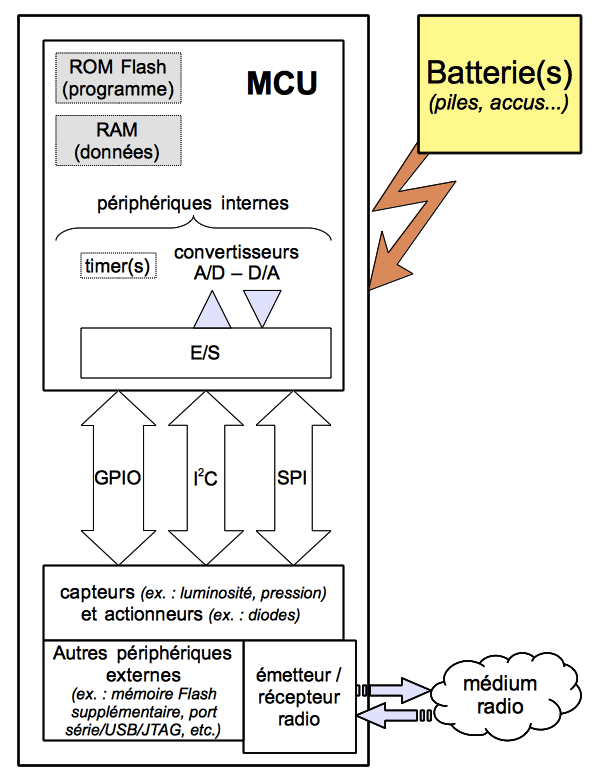
\includegraphics[width=11cm]{images/ch2-structure-mote.png}
\flcaption{Schéma fonctionnel d'une \lang{mote} WSN~/ IoT classique.}
\label{FigStructMote}
\end{figure}

Les motes constituant les \nom{noeuds} des WSN~--- et par extension
de l'IoT~--- sont des appareils extrêmement compacts~: ils sont conçus
autour d'un circuit intégré central regroupant le processeur principal
(CPU) et plusieurs périphériques de base intégrés~: \lang{timers},
convertisseurs A/D et D/A, contrôleurs E/S regroupant des broches à
usage général, des bus SPI et I$^2$C, etc. Ces circuits intégrés
centraux sont appelés \nom{microcontrôleurs} (\nom{MCU}: \lang{Micro
Controller Unit}).

Il faut être bien conscient que ces MCU disposent d'une puissance
de calcul et d'un espace mémoire extrêmement limités~--- non seulement
comparés aux ordinateurs personnels (PC) actuels, mais également en
regard d'appareils mobiles tels que les \lang{smartphones} et les
tablettes. Leur puissance est en fait plutôt comparable, pour les
modèles les moins chers (et donc parmi les plus couramment employés),
à celle des ordinateurs personnels du début des années 1980 (Apple II,
Commodore VIC et 64, Atari 800XL, Amstrad CPC, etc.).

Outre ce MCU central, une \lang{mote} comprend en général seulement
quelques \nom{capteurs} (\lang{``sensors''})~--- et parfois, plus
rarement quelques \nom{actionneurs} (\lang{``actuators''})~--- leur
permettant d'interagir avec leur environnement, en captant et mesurant
des phénomènes physiques environnants~--- température, pression, humidité,
présence d'individus, radioactivité...~; l'ensemble des capteurs
envisageables est quasiment sans limite~--- et en agissant sur
cet environnement pour les \lang{motes} équipées d'actionneurs
(par exemple~: alarme, signaux lumineux, etc.)

De nombreuses \lang{motes} possèdent, pour des raisons pratiques, des
périphériques supplémentaires (externes au MCU)~: on citera par exemple
de la mémoire Flash supplémentaire pour le stockage permanent de
données, ou des ports série~/ USB pour se connecter à un PC~---
principalement à des fins de déboguage.

Une \lang{mote} est bien évidemment équipée d'un émetteur~/
récepteur radio, pour pouvoir communiquer en réseau. Comme dit
ci-dessus, ces appareils sont pour la plupart extrêmement limités
en énergie~; ces émetteurs~/ récepteurs radio utilisent donc un
standard conçu pour consommer très peu d'énergie, en contrepartie
d'un débit très limité (comparable aux premiers modems analogiques du
début des années 1990). La standard spécifiquement conçu dans cette optique
utilisé par la plupart de ces radios est le standard IEEE 802.15.4
\cite{IEEE802154-2011} (ne couvrant que les couches les plus basses
de la pile réseau) que nous décrirons ultérieurement dans le
présent manuscrit en section \vref{SecProto802154}. Notons que
certains MCUs récents, dans un souci d'efficacité et d'intégration,
intègrent directement un émetteur~/ récepteur radio sur la même puce.

Enfin, une \lang{mote} est bien évidemment équipée d'une ou plusieurs
batteries pour son alimentation. Certains modèles de développement~/
déboguage offrent également la possibilité d'être alimentés par une
source d'énergie externe (secteur).

\paragraph{Les middlewares pour WSN.}
\label{ParMiddlewares}

Avant de nous intéresser en détail au fonctionnement technique des couches
de bas niveau des WSN, nous allons très brièvement évoquer un autre
sujet de recherche actif dans le domaine des WSN.

Notons en effet que l'absence de standard officiel pour les WSN au-delà
des deux couches les plus basses fournies par le standard IEEE 802.15.4
(niveaux OSI 1~: PHYsique, et 2~: \lang{Media Access Control}, comme
nous le verrons dans la section \vref{SecProto802154} de l'état
de l'art) a amené à un développement assez anarchique des piles, protocoles
et autres solutions pour les couches plus hautes. À l'heure où nous écrivons
ces lignes, aucune des solutions conçues pour travailler par-dessus les
réseaux 802.15.4 (telles ZigBee, etc.) ne s'est réellement imposée comme
standard, fut-il de fait.

On voit donc, selon les applications prévues pour les différents WSN,
se multiplier des solutions souvent incompatibles dans le déploiement
des différents réseaux de capteurs sans-fil sur le terrain.

Un domaine de recherche dans les WSN est donc la conception de
\emph{``middlewares''} (<<~intergiciels~>>) permettant une interaction
efficace entre tous ces WSN de conception différente et le réseau global
(Internet), pour tenter de faire de l'IoT une réalité tangible, fiable et
donc utilisable industriellement. Un article de référence (\lang{``survey''})
recensait déjà nombre de projets de ce type lors de la décennie précédente
\cite{Middleware-WSN-Survey-2008}.

Nous n'avons au cours de cette thèse malheureusement quasiment pas
eu le temps de nous pencher sur cette problématique, si ce n'est au
début pour travailler très brièvement sur le \lang{middleware} MPIGate
\cite{KR-UbiMob-2013}. Les travaux de la présente thèse concernent,
à l'exception de la publication cité dans la phrase précédente,
uniquement les couches basses des piles réseau des plates-formes
spécialisées pour WSN.


\subsection{Les réseaux de capteurs sans-fil et leur trafic}
\label{SubsecTraficWSN}

Les réseaux de capteurs sans-fil (WSN) sont, comme nous l'avons vu
ci-dessus dans le descriptif des motes, des réseaux à bas débit et
à faible portée, en contrepartie d'une consommation d'énergie très
limitée.

Le trafic réseau est, dans ce genre de réseau, typiquement faible,
avec éventuellement des pointes de débit. Les transmissions entre
noeuds d'un WSN peuvent, par nature, être déclenchées selon trois
modalités différentes~:

\begin{description}

\item[Périodique~:] un noeud capteur analyse son environnement à
intervalles réguliers, en tire une valeur exploitable (par exemple~:
température, pression, etc.), et l'émet sur le réseau à l'aide
de son émetteur~/ récepteur radio. L'intervalle de temps entre
deux mesures~/ émissions est à la discrétion des concepteurs
du WSN et~/ ou des programmeurs de la \lang{mote}.

\item[\'Evènementiel~:] un noeud capteur, lors d'une analyse de
son environnement, capte une valeur~--- ou une variation de valeur~---
anormale ou atypique, et envoie alors un message d'alerte sur le
réseau. Là encore, l'intervalle des valeurs normales, ou le type
d'évènement susceptible de déclencher l'envoi d'une alerte est
à la discrétion des concepteurs du WSN et/ou des programmeurs
de la \lang{mote}.

\item[Par requête~:] un intervenant extérieur au WSN émet, via
la station de base\footnotemark[1] une requête vers une \lang{mote}
donnée, qui y répond par le déclenchement d'un actionneur~--- si
le noeud en est équipé~--- et~/ ou par l'envoi d'une réponse,
correpondant le plus souvent à une valeur analysée par un des
capteurs de la \lang{mote} en question. Ici aussi, la nature des
requêtes et des réponses à y apporter sont à la discrétion des
concepteurs du WSN et/ou des programmeurs de la \lang{mote}.

\footnotetext[1]{La \nom{station de base} est le noeud (\lang{mote}
ou PC ou tout autre appareil connecté) servant de lien entre un
réseau de capteurs sans-fil et le reste de l'Internet~: il s'agit,
pour faire simple, des passerelles de l'Internet des Objets (IoT).
On les nomme également souvent \nom{\lang{``sinks''}}.}

\end{description}

Ces trois modalités ne sont bien évidemment pas exclusives~: un même
WSN peut utiliser les trois types de fonctionnement en fonction des
besoins du moment.

Prenons l'exemple, pour aborder le sujet de l'e-santé qui concerne
cette thèse, d'un WSN destiné à monitorer les signes vitaux d'un
patient sous surveillance (par exemple~: un malade cardiaque)~:

\begin{itemize}

\item En temps normal, les capteurs présents sur le patient relèvent
ses signes vitaux (pulsations cardiaques, pression sanguine, oxymétrie
de pouls, mouvements respiratoires, etc.) de façon régulière et
envoient ainsi (via l'IoT) les résultats à une base de données
spécialisée consultable par les médecins.

\item En cas d'anomalie, (par exemple~: chute de pression sanguine,
ou des pulsations), les capteurs envoient sans attendre un message
d'alerte, qui pourra être relayé aux médecins traitant le patient
ou même, selon la gravité, au SAMU. Un mécanisme d'IoT permettant
d'envoyer des messages (type SMS) à des secouristes présents à
proximité du patient pourrait également être envisagé.

\item En cas de situation critique (par exemple~: fibrillation
cardiaque), les messages d'alerte envoyés plus tôt auront alerté
les services médicaux d'urgence, qui pourront en attendant l'arrivée
physique des secours envoyer (toujours via l'IoT) une requête au WSN
présent sur le patient~: par exemple pour ordonner la mise en action
d'un défibrillateur cardiaque portatif (ou d'un \lang{``pace-maker''})
connecté au WSN porté par le patient.

\end{itemize}

Les possibilités offertes par les WSN~--- ne serait-ce que sur le seul
domaine médical vu dans cet exemple~--- sont donc extrêmement larges.

Il importe toutefois, pour connaître les limites de ces réseaux
de capteurs sans-fil, d'en connaître les spécificités. C'est le
sujet que nous allons maintenant aborder dans la prochaine section.


\subsection{Spécificités des WSN}
\label{SubsecSpecifWSN}

Par rapport aux réseaux traditionnnels, les réseaux de capteurs sans-fil
ont des spécificités, décrites dans la table \vref{TabComparResWSN}.

\begin{table}[!p]
\centering
\begin{tabular}{|p{5.9cm}|p{5.9cm}|}
\hline
\textbf{Réseaux traditionnels}
 & \textbf{Réseaux de capteurs sans-fil} \\
\hline
\emph{Réseaux généralistes~:} conçus pour servir toutes les applications
possibles.
& \emph{Réseaux spécifiques~:} conçus dans un but unique pour servir une
application bien définie.\\
\hline
Les principaux objectifs sont \emph{la performance du réseau et ses
latences}. La consommation d'énergie n'est pas une préoccupation
majeure.
& \emph{L'énergie est une contrainte centrale} dans la conception d'un
réseau de capteurs sans-fil et de chacun de ses noeuds.\\
\hline
Les réseaux sont \emph{conçus et déployés selon des plans pré-déterminés}.
& Le déploiement, la structure des réseaux et l'utilisation des ressources
sont souvent déterminés de manière \nom{ad-hoc} \emph{(sans planification
préalable)}.\\
\hline
Les réseaux et leurs composants opèrent dans des \emph{environnements
contrôlés} et des \emph{conditions environnementales modérées}.
& Les réseaux de capteurs sans-fil opèrent souvent dans des 
\emph{environnements et des conditions hostiles}.\\
\hline
La maintenance et la réparation sont des opérations courantes et
\emph{le réseau et ses composants sont typiquement faciles d'accès.}
& \emph{L'accès physique aux capteurs sans-fil est souvent difficile
voire même impossible}.\\
\hline
\emph{Le coût des composants des réseaux peut être élevé}, selon le
niveau de performances visé.
& \emph{Le coût des capteurs sans-fil doit rester très faible}, d'où le
recours à des composants bon marché aux performances (et parfois à la
fiabilité) limitées.\\
\hline
La défaillance d'un composant du réseau est réglée par \emph{des
opérations de maintenance et de réparation}.
& La défaillance d'un ou plusieurs noeuds est prévisible et
\emph{gérée dans la conception même du réseau}.\\
\hline
La connaissance de l'état global du réseau est typiquement possible
et \emph{la gestion centralisée est possible}.
& La plupart des décisions sont \emph{prises au niveau local sans
intervention d'une gestion centralisée}.\\
\hline
\end{tabular}
\flcaption{Comparaison entre réseaux traditionnels et WSN.
(d'après \cite{LivreDargie2010} table 1.2)}
\label{TabComparResWSN}
\end{table}

\bigskip

Les principaux points déterminants concernant ces spécificités sont les
suivants~:

\begin{itemize}

\item Les capteurs sans-fil sont des appareils dont le coût doit rester
le plus faible possible. Cela influe sur les capacités très limitées
de ces appareils, et aussi potentiellement sur leur fiabilité.

\item Les réseaux de capteurs sans-fil sont généralement des réseaux
\emph{ad-hoc}, c'est-à-dire dont la structure n'est pas planifiée.
Leur mode de fonctionnement est ainsi fondamentalement local, aucune
gestion centralisée n'est en général possible.

\item Les réseaux de capteurs sans-fil sont en général conçus pour
servir une et une seule application donnée au cours de leur existence
(point commun avec l'informatique~/ électronique embarquée). Ils
peuvent être amenés à opérer dans des conditions environnementales
difficiles voire hostiles.

\item Un point commun avec les réseaux traditionnels est la montée
en charge. Un réseau de capteurs sans-fil peut résulter de l'interconnexion
de centaines de PANs, et regrouper ainsi des milliers de \lang{motes}.
De telles tailles de réseau sont rarement atteintes avec les réseaux
sans-fil les plus courants.

\item Les noeuds de ces réseaux pouvant tomber en panne sans pouvoir
être remplacés (défaillance d'un composant, ou d'une batterie non
remplaçable), la structure de tels réseaux doit pouvoir <<~survivre~>>
à ces pannes et les gérer.

\item Ce sont des réseaux sans-fil, dont le médium radio est peu fiable
par nature (par rapport aux réseaux câblés), sujet à la diffusion, et
dont l'état est variable au cours du temps.

\item Enfin, et c'est peut-être le plus important, la consommation
d'énergie est une contrainte extrêmement forte dans les réseaux de capteurs
sans-fil, bien plus que dans n'importe quel autre type de réseau. Cette
contrainte influe directement et lourdement sur la conception des WSN
et de leurs noeuds.

\end{itemize}

\bigskip

Pour répondre à ces différents problèmes, quatre notions liées à
\emph{l'auto-gestion} sont mises en avant dans \cite{LivreDargie2010}
comme caractéristiques désirables pour les WSN~:

\begin{description}

\item[\lang{``Self-organization''},] \nom{auto-organisation~:}
est la capacité d'adapter les paramètres de la configuration du réseau
en fonction de son état et de son environnement.

\item[\lang{``Self-optimization''},] \nom{auto-optimisation~:}
est la capacité de monitorer et d'optimiser l'utilisation des ressources
limitées du réseau.

\item[\lang{``Self-protection''},] \nom{auto-protection~:}
est la capacité de reconnaître les intrusions et attaques et de s'en
protéger.

\item[\lang{``Self-healing''},] \nom{auto-réparation~:}
est la capacité de découvrir, d'identifier la cause et de réagir aux
pannes et défaillances du réseau.

\end{description}

Ces différentes notions amènent à la capacité de ces réseaux de capteurs
sans-fil d'assurer un niveau de service suffisant pour les applications
ayant des contraintes fortes quant à la qualité et le débit de leurs
flux de données. Ce domaine, la \nom{Qualité de Service (QdS)} (\lang{QoS}
en anglais) va être l'objet d'étude de la prochaine section \ref{SecQdS}.

%%%%%%%%%%%%%%%%%%%%%%%%%%%%%%%%%%%%%%%%%%%%%%%%%%%%%%%%%%%%%%%%%%%%%%%%%%%%%

\section{La Qualité de Service (QdS)}
\label{SecQdS}

Note~: cette section est inspirée des informations issues de
\cite{TheseBNefzi} et de \cite{CCMQdS}


\subsection{Notion de QdS}
\label{SubsecDefQdS}

Le terme \nom{QdS} (\nom{<<~Qualité de Service}, en anglais QoS:
\lang{``Quality of Service''}) désigne la capacité à fournir un service,
ici un support de télécommunications, conforme à des exigences de
fonctionnement acceptable à assurer par le fournisseur du service
envers l'utilisateur.

Appliquée aux réseaux à commutation de paquets (réseaux basés sur
l'utilisation de routeurs) la QoS désigne l'aptitude à pouvoir garantir
le non-dépassement d'un niveau acceptable de baisse de qualité, défini
contractuellement, pour un usage donné (voix sur IP, vidéo-conférence, etc.).

En effet, contrairement aux réseaux à commutation de circuits, tels que
le réseau téléphonique commuté, où un circuit de communication est dédié
pendant toute la durée de la communication, il est impossible sur Internet
de prédire le chemin emprunté par les différents paquets.

Cette incertitude est encore plus forte sur les réseaux sans-fil,
où le médium radio lui-même est sujet à la diffusion, dont l'état
et l'encombrement peuvent varier fortement et rapidement au cours
du temps. Ce médium est, comparé aux câbles des réseaux informatiques
<<~classiques~>>, bien moins fiable.

Ainsi, rien ne garantit qu'une communication nécessitant une régularité
du débit pourra avoir lieu sans encombre. C'est pourquoi il existe des
mécanismes, dits mécanismes de QoS, permettant de différencier les
différents flux réseau et réserver une partie de la bande passante
pour ceux ayant une importance particulière.

Plus formellement, la recommandation E.800 de septembre~2008 de l'Union
Internationale des Télécommunications (UIT) définit la QdS comme étant
<<~l'ensemble des caractéristiques d'un service de télécommunication qui
lui permerrent de satisfaire aux besoins explicites et aux besoins
implicites de l'utilisateur du service~>>~; une caractéristique étant
définie comme une <<~propriété (qualitative ou quantitative) qui aide
à faire la distinction entre les individus d'une population donnée~>>.

En termes pratiques, une caractéristique du standard E.800 de l'UIT
correspond à un critère de QdS. Le but à atteindre étant d'assurer
une valeur minimale en-deça de laquelle ne pas tomber pour respecter
un contrat de qualité avec l'utilisateur.

\newpage


\subsection{Critères de QdS}
\label{SubsecCritQdS}

Les principaux critères permettant d'apprécier la qualité de service
sont les suivants~:

\begin{description}

\item[Perte de paquets] (en anglais \lang{packet loss})~: elle
correspond à la non-délivrance (perte) de paquets de données, la plupart
du temps dûe à un encombrement du réseau.

\item[Débit] (en anglais \lang{bandwith})~--- encore appelée \nom{bande
passante}~--- il définit le volume maximal d'information (bits) pouvant
transiter par unité de temps.

\item[Latence, délai, ou temps de réponse] (en anglais \lang{delay})~:
elle caractérise le retard entre l'émission et la réception d'un
paquet de données.

\item[Gigue] (en anglais \lang{jitter})~: elle représente la fluctuation
du signal numérique, dans le temps ou en phase.

\item[Déséquencement] (en anglais \lang{desequencing})~: correspond à
une modification de l'ordre d'arrivée des paquets.

\end{description}

Le rôle d'une politique ou d'un mécanisme de QdS est de toujours garder
une valeur acceptable (égale ou supérieure à une valeur-seuil de
qualité minimale) pour ces différents critères.

(\`A noter qu'à côté de ces principaux critères de QdS, d'autres peuvent
être pris en compte, comme par exemple la durée de vie de chaque noeud,
le MTBF, le respect du coût, etc.)

\subsection{Stratégies d'assurance de la QdS}
\label{SubsecStratQdS}

Les stratégies classiques appiquées pour assurer une QdS optimale
peuvent se diviser en deux grandes catégories~:

\begin{itemize}

\item Les méthodes de contrôle \lang{a priori} ou \emph{préventives}
du trafic réseau que sont~:
  \begin{itemize}
  \item les politiques de gestion de files d'attente, ou ordonnancement,
        permettant la mise en place de la différentiation de service~;
  \item le lissage (ou mise en forme) du trafic, consistant à contrôler
        le volume du trafic entrant dans le réseau, la plupart du temps
        selon les méthodes du seau percé ou du seau à jetons~;
  \item le contrôle du trafic, et sa variante extrême, le contrôle
        d'admission, consistant à refuser le trafic entrant en
        fonction de certains critères.
  \end{itemize}

\item Les méthodes de contrôle \lang{a posteriori} ou \emph{réactives}
du trafic réseau~:
  \begin{itemize}
  \item le contrôle de congestion, acceptant tout le trafic arrivant
        en conditions normales, et diminuant le débit ou supprimant
        des paquets lors de la survenue d'une congestion~; le mécanisme
        de fenêtre de congestion de TCP~/ IP fait partie de ces méthodes~;
  \item le choix dynamique des routes, pour assurer la meilleure QdS
        possible en fonction de l'état courant d'un réseau~: ce
        mécanisme dépend du protocole de routage de la pile réseau.
  \end{itemize}

\end{itemize}

D'une façon générale, les méthodes de contrôle réactives semblent se
montrer mieux adaptées aux réseaux sans-fil, notamment aux WSN, les
méthodes proactives s'adaptant mal au médium radio et ses caractéristiques.


\subsection{Niveaux de service}
\label{SubsecNivQds}

Le terme \nom{niveau de service} (en anglais \lang{Service level}) définit
le niveau d'exigence pour la capacité d'un réseau à fournir un service
point à point ou de bout en bout avec un trafic donné. On définit
généralement trois niveaux de QdS :

\begin{description}

\item[Service garanti] (en anglais \lang{guaranteed service} ou 
\lang{hard QoS}), consistant à réserver des ressources réseau pour certains
types de flux. Le principal mécanisme utilisé pour obtenir un tel niveau
de service est RSVP (\lang{Resource reSerVation Protocol}, en français
<<~Protocole de réservation de ressources~>>).

\item[Service différencié] (en anglais \lang{differenciated service} ou
\lang{soft QoS}), permettant de définir des niveaux de priorité aux
différents flux réseau sans toutefois fournir une garantie stricte.

\item[Meilleur effort] (en anglais \lang{best effort}), ne fournissant
aucune différenciation entre plusieurs flux réseaux et ne permettant
aucune garantie. Ce niveau de service est ainsi parfois appelé
(abusivement) \lang{lack of QoS}.

\end{description}


\subsection{QdS dans les réseaux de capteurs sans-fil}
\label{SubsecQdsWSN}

Les données venant d'être exposées jusqu'ici dans la présente section
\ref{SecQdS} concernent la QdS en général~: elles s'appliquent à tous
les types de réseaux.

Pour les réseaux de capteurs sans-fil, la nature même du réseau, avec
des noeuds aux capacités très limitées, une contrainte énergétique
très forte, un médium radio non-fiable, et une possibilité de défaillance
de noeuds, rend les notions de service garanti ou différencié impossibles
à atteindre. \emph{La Qualité de Service, dans le domaine des WSN,
est donc quasiment toujours une garantie du type \lang{``best effort''}}.

Concernant les critères de QdS importants et gérés au niveau des
couches MAC~/ RDC des WSN, on s'intéresse principalement au
\emph{taux de perte de paquets} et au \emph{délais de transmission}.
Les autres critères étant soit définis par les standards gérant
le médium radio~--- par exemple~: le débit (théorique) de 250~Kbit/s
pour le standard 802.15.4 sur la bande 2,4 GHz~---~; soit dépendants
de conditions externes sur lesquelles aucune intervention n'est possible
(gigue, débit réel diminué par des interférences radio)~; soit réglés
par les couches supérieures des piles réseau (déséquencement des paquets).

Enfin, le caractère extrêmement contraignant de la limitation énergétique
fait de cette \emph{obligation d'économie d'énergie un critère à part
entière de la QdS}~--- bien que celui-ci soit contradictoire avec les
autres critères de QdS. En effet, les \lang{motes} étant souvent dans
des situations où le changement de batterie est difficile ou même impossible,
conserver la batterie opérationnelle le plus longtemps possible revient à
maintenir le noeud correspondant <<~en vie~>> le plus longtemps possible.
Une \lang{mote} à cours d'énergie est en effet souvent une \lang{mote}
perdue définitivement, donc une perte de fonctionnalité~--- potentiellement
sévère~--- pour le WSN correspondant.

En résumé, on peut dire que pour les WSN, le lien entre Qualité de Service
<<~fonctionnelle~>> (bande passante, fiabilité et rapidité des transmissions)
et économie d'énergie est tout à la fois contradictoire, indissociable
et crucial. L'optimisation de la QdS revient ainsi toujours à trouver
\emph{le meilleur compromis, l'équilibre optimal} entre tous les facteurs
cités dans cette présente section \ref{SubsecQdsWSN}, en fonction de
l'application voulue.

\bigskip

Après toutes ces définitions techniques, nous allons maintenant dans la
section \ref{SecAppWSN} suivante passer en revue les différents domaines
d'applications des WSN. Comme nous allons le voir, ceux-ci sont nombreux
et variés.

%%%%%%%%%%%%%%%%%%%%%%%%%%%%%%%%%%%%%%%%%%%%%%%%%%%%%%%%%%%%%%%%%%%%%%%%%%%%%

\section{Applications des WSN (et de l'IoT)}
\label{SecAppWSN}

Akyildiz et Vuran, dans leur livre \cite{LivreAkyildiz2010}, considèrent
cinq grands types d'applications aux WSN (voir figure
\vref{FigAppWSNAkyildiz})~:

\begin{figure}[hbt]
\centering
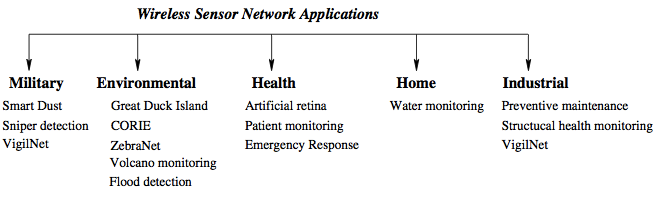
\includegraphics[width=12.5cm]{images/ch2-app-wsn.png}
\flcaption{Principales catégories d'application des réseaux de
capteurs sans-fil.
Source~: \cite{LivreAkyildiz2010}, figure 2.1.}
\label{FigAppWSNAkyildiz}
\end{figure}

\begin{description}

\item[Applications militaires~:] les buts sont multiples, comme le contrôle
des forces alliées, de leur équipement et de leurs munitions, la surveillance
du champ de bataille, la reconnaissance de l'ennemi et du terrain,
l'évaluation des dégâts, ou la détection d'attaques non conventionnelles.
Plusieurs exemples sont cités dans \cite{LivreAkyildiz2010}~: le projet
\lang{Smart Dust} du DARPA (un pionnier dans les WSN), ou un système de
détection de \lang{sniper} \footnotemark[2].
\footnotetext[2]{Démontrations vidéos sur cette page Web~:
\texttt{http://bbn.com/boomerang}}

\item[Applications industrielles~:] ici aussi, les applications sont
nombreuses~: la supervision des processus de fabrication et la vérification
de la qualité de production, la localisation et la surveillance de
l'équipement industriel, la maintenance préventive des usines (surtout de
grande taille) et des conditions de travail ou d'opération du matériel
industriel, etc. Un exemple cité dans \cite{LivreAkyildiz2010} est
le projet FabApp \cite{FabApp}, dont le but est d'évaluer les vibrations
du matériel industriel lors de son fonctionnement pour prévenir
pannes et accidents (tant dans une usine de fabrication de semi-conducteurs
que dans un pétrolier).\\
On pourra également citer des applications de contrôle de l'état structurel
des bâtiments, comme par exemple la surveillance active du \lang{Golden Gate
Bridge} (San Francisco) \cite{AppGoldenGate}.\\
Citons aussi l'assistance au domaine minier~: l'objectif étant de détecter
les évènements dangereux pour les mineurs (poches de gaz, responsables
de <<~coups de grisou~>>) ainsi que de quantifier les émissions de méthane
produites par les mines de charbon (le méthane étant un gaz à effet de
serre, celui-ci influe sur le changement climatique actuel).

\item[Applications environnementales~:] de nombreux projets sont
réalisables, comme le suivi des mouvements d'animaux, la détection de feux
de forêts ou d'inondations, la recherche météorologique ou géophysique,
l'étude de la pollution, etc. Plusieurs exemples sont cités dans
\cite{LivreAkyildiz2010}, parmi lesquels~: \lang{ZebraNet} \cite{ZebraNet}
un système de surveillance au long cours de la population de zèbres,
déployé au Kenya. Autre exemple~: un système de surveillance des volcans
\cite{VolcansWSN}~--- également cité dans \cite{LivreDargie2010}~---
le but étant ici de détecter à l'avance les signes avant-coureurs des
éruptions, pour mieux prévenir celles-ci, ou d'étudier le fonctionnement
de volcans sous-marins, pour mieux comprendre les phénomènes d'activité
volcanique. On peut aussi citer un système de détection précoce
d'inondations dans les pays en voie de développement \cite{FloodDetect}.\\
Les réseaux de capteurs sans-fil servent également à l'agriculture de
précision, en permettant d'analyser précisément l'état des sols, afin de
mieux utiliser les ressources à utiliser (eau, engrais, pesticides,
herbicides) pour optimiser les récoltes. Plusieurs projets prototypes
ont déjà été déployés dans ce but.\\
L'environnement urbain peut également en bénéficier, par exemple par des
applications de contrôle actif du trafic routier aux \'Etats-Unis
\cite{ControleTrafic}, ou encore le projet PipeNet \cite{PipeNet}
mis en place dans de nombreuses villes américaines pour monitorer
les réseaux d'égoûts.

\item[Applications à la santé~:] le domaine de la santé fait partie du
contexte de la présente thèse, et nous y reviendrons donc plus longuement
dans une section suivante (section \vref{SubsecSanteWSN}).

\item[Applications domotiques~:] On cite dans \cite{LivreAkyildiz2010}
un système nommé NAWMS \cite{NAWMS} destiné à détecter les gaspillages
d'eau et leur origine précise, afin d'en informer les usagers pour
les aider à réduire leur facture d'eau.

\end{description}

En étudiant les applications des WSN et de l'IoT citées dans
\cite{LivreDargie2010} et \cite{LivreAkyildiz2010}, on voit que ces
applications ne manquent pas, et sont appelées à continuer à se développer
de façon exponentielle.

\newpage

Nous allons maintenant dans la section \ref{SecContexte} suivante
nous focaliser sur le contexte de la présente thèse.

Ce contexte est celui du domaine d'application de la santé pour les WSN.
Nous y étudierons tout particulièrement le projet LAR (\lang{``Living
Assistant Robot''}), dont cette thèse fait partie, dans la section
\vref{SubsecLAR}.

%%%%%%%%%%%%%%%%%%%%%%%%%%%%%%%%%%%%%%%%%%%%%%%%%%%%%%%%%%%%%%%%%%%%%%%%%%%%%

\section{Contexte}
\label{SecContexte}


\subsection{Applications d'e-santé des WSN}
\label{SubsecSanteWSN}

L'utilisation des réseaux de capteurs sans-fil pour des applications
dans le domaine de la santé est un domaine déjà bien établi et très
actif~: les PAN (\lang{Personal Area Network}) dédiés à être installés
sur un patient~--- par exemple pour suivre son état de santé~--- sont
même désignés par un acronyme spécifique~: \nom{BAN} \emph{(\lang{``Body
Area Network''})}.

Les applications des WSN au domaine de la santé sont également, comme dans
les autres domaines, très nombreuses et variées~: un article complet
de référence \cite{WSN-HealthCare-Survey-2010} recensait en 2010 les
nombreux projets d'exploitation des réseaux de capteurs sans-fil liés
au domaine de la santé.

Parmi les projets les plus ambitieux, les deux livres de
\cite{LivreDargie2010} et de \cite{LivreAkyildiz2010} citent tous deux des
projets de rétines artificielles \cite{RetineArtificielle}
\cite{RetineArtificielle2} combinant une caméra CCD externe couplée à des
nano-noeuds sans-fil implantés \emph{in vivo} sur la rétine du patient.
Ces projets visent à apporter une solution à des maladies actuellement
incurables, comme la DMLA (Dégénérescence Maculaire Liée à l'Âge) ou
la rétinite pigmentaire (maladie génétique).

Sans aller jusqu'à des projets aussi avancés technologiquements (et
organiquement invasifs) de nombreux projets de surveillance à domicile
de patients fragiles et de réponse aux cas d'urgence sont actuellement
mis en place.

Rappelons notamment l'existence du projet \nom{d'informatique située},
consistant en une plate-forme d'<<~appartement intelligent pour l'assistance
à la personne~>> \cite{AppartIntelligent}, utilisant intensivement les WSN,
que l'on peut classer à la fois dans les applications domotiques et les
applications à la santé. Ce projet, hébergé au LORIA~/ INRIA Nancy Grand-Est,
implique directement (entre autres) notre équipe~--- Madynes~---, et l'un
des encadrants de la présente thèse~--- Y.-Q. Song.


\subsection{Le projet LAR}
\label{SubsecLAR}

Un autre de ces projets fait également usage des WSN, combinant aussi~---
comme nous l'avons dit auparavant au chapitre \ref{ChIntro}~--- aspect
domotique et aspect santé, est le \nom{projet LAR} (\lang{``Living Assistant
Robot''}), dont la présente thèse fait partie.

\newpage

Le projet LAR a pour objectif d'aider au maintien à domicile des personnes
âgées et~/ ou dépendantes, et de tenter de retarder le plus possible le
moment où ces dernières doivent être placées en institutions spécialisées,
ce qui représente un coût financier et surtout humain considérable.

Dans ce but, le projet vise à fournir des outils de suivi à domicile
de la personne dépendante et de son activité, de développer pour cela
des outils de perception, de modélisation de l'activité humaine,
et d'interaction avec la personne. Comme le nom du projet l'indique,
il est question de fournir (du moins dans le cas les plus lourds)
un robot d'assistance spécialement conçu par le projet~; mais une
grande partie du travail fourni (détection de présence, de mouvement,
de chutes, etc.) sera fourni par un ou plusieurs WSN installés chez
le patient, le robot étant également porteur de capteurs et actionneurs
et donc membre à part entière de ce(s) WSN. Ces WSN sont également reliés
à l'IoT, les données médicales recueillies étant destinées à être
stockées dans des bases médicales spécialisées, accessibles de façon
sécurisée aux personnels de soins (médecins, infirmiers, etc.).

Le principe central du projet LAR est la mise en {\oe}uvre d'un écosystème
modulaire de services (comme nous venons de le voir~: capteurs de données
de toutes natures, robots, mais aussi services à la personne, etc.),
lesquels services opèrent au sein d'une architecture orientée services
(\lang{``Service Oriented Architecture''} ou \nom{SOA}) centrée sur un
orchestrateur (alias \lang{``Enterprise Message Bus''}) Microsoft BizTalk.

L'un des objectifs fondamentaux du projet est de commercialiser ce
service au coût le plus faible possible, afin de le rendre accessible
au plus grand nombre~; c'est pourquoi le recours à des WSN (avec leurs
\lang{motes} à faible coût) est un point clé du programme. L'une des
idées directrices du projet est de rendre l'offre modulaire, et de ne
fournir que les services nécessaires à l'état courant du patient~:
les cas les plus légers n'auront ainsi que l'installation d'un WSN
<<~léger~>> et peu intrusif à leur domicile, l'évolution de l'état
du patient pouvant ensuite amener à recourir à des modules
supplémentaires~; le robot étant l'élément le plus évolué mais aussi
le plus coûteux.

Plusieurs partenaires académiques et industriels sont impliqués dans
ce projet~: la partie académique est représentée par le LORIA~/ INRIA
Nancy Grand-Est en l'équipe Madynes (dont nous faisons partie) pour les
WSN, et l'équipe Larsen~--- anciennement Maia~--- pour la partie robotique
et reconnaissance des mouvements~; les partenaires industriels sont
Diatelic (pour la gestion de la base de données médicales et son accès
sécurisé), Robosoft S.A. (pour la conception et la fabrication du robot),
et le Pôle Innovation du Crédit Agricole S.A. (qui coordonne le projet).
Tous ces partenaires ont formé un consortium~--- dont le Crédit Agricole
a pris la tête~--- pour répondre à l'appel d'offres <<~e-santé~>> lancé
en 2011 par la DGCIS~--- depuis devenue DGE (Direction Générale des
Entreprises)~---, lequel consortium a remporté l'appel et ainsi fondé
le projet LAR. Le contrat correspondant a été signé en 2012, et le projet
LAR a été financé par la Banque Publique d'Investissement (BPIFrance).

%%%%%%%%%%%%%%%%%%%%%%%%%%%%%%%%%%%%%%%%%%%%%%%%%%%%%%%%%%%%%%%%%%%%%%%%%%%%%

\section{Problématique}
\label{SecProblematique}


\subsection{Exposé de la problématique}
\label{SubsecExposeProblematique}

Dans le domaine des réseaux de capteurs sans-fil, les piles réseau
spécialisées constituent un domaine de recherche très actif depuis
maintenant une quinzaine d'années. On citera actuellement, par exemple
dans le domaine des couches hautes, les protocoles de routage (RPL et ses
nombreuses variantes et évolutions), ou encore l'activité actuelle autour
des CCN (\lang{``Content-Centric Networks''}).

Pour les couches basses, de nombreux travaux de recherche ont également
été effectués sur les protocoles MAC (la couche MAC représentant le
niveau 2 dans le modèle OSI), pour suppléer le protocole du
standard 802.15.4 et ses limitations, comme nous le verrons au
chapitre \vref{ChEtatArt}. Toutefois, beaucoup de ces études se
sont principalement consacrées à l'étude théorique de ces protocoles,
se contentant souvent~--- à des fins de tests~--- de simulations
puremement théoriques (avec des outils comme OPNET, ns-3, OMNeT++, voire
même MATLAB), ou au mieux par des émulations de \lang{motes} virtuelles
(avec des outils comme TOSSIM \cite{TOSSIM} ou Cooja \cite{Cooja}).

L'implantation de ces couches basses, dans les plates-formes logicielles
réelles~--- c'est à dire les systèmes d'exploitation dédiés aux réseaux de
capteurs sans-fil~--- n'a pas fait l'objet d'un effort de recherche poussé
et systématique. Le principal but était de minimiser la consommation
d'énergie de ces couches basses, généralement en ayant recours aux
protocoles et aux implantations les plus simples possibles.

L'un des seuls efforts remarquables de conception et d'implantation
dans ce domaine, le protocole ContikiMAC~--- développé spécifiquement
pour la plate-forme logicielle Contiki OS~--- a ainsi comblé un manque,
et est devenu le standard de fait, du moins dans la littérature sur le
domaine des réseaux de capteurs sans-fil. Depuis, on ne peut qu'observer
un certain \lang{statu quo} dans ce domaine. Si de nombreux protocoles
MAC à hautes performances ont été conçus (comme nous le verrons dans
la section \vref{SecProtoMAC} de l'état de l'art), aucun d'entre
eux n'a été implanté et largement diffusé avec un OS spécialisé
comme l'est ContikiMAC.


\subsection{Stratégie préconisée}
\label{SubsecStrategieThese}

\subsubsection{Besoins identifiés}
\label{ParBesoins}

Pour avancer dans ce domaine, et notamment pouvoir exploiter les
nouvelles \lang{motes} plus puissantes~--- par exemple celles basées
sur des microcontrôleurs à base ARM Cortex-M~--- rencontrées de plus
en plus souvent (en sus des plates-formes classiques à base MSP430
ou AVR), nous voyons plusieurs besoins à combler~:

\begin{enumerate}

\item \emph{Faire évoluer les plates-formes logicielles (OS) spécialisées
dans les réseaux de capteurs sans-fil, en leur ajoutant des
fonctionnalités nécessaires au développement de piles réseau plus
performantes.}\\
La programmation sans OS ni plate-forme d'aucune sorte (programmation
\lang{``bare metal''}) nous semble à proscrire, car les logiciels ainsi
créés ne sont nullement portables, et doivent être réécrits à chaque
changement de matériel, lequel dans ce domaine (comme dans toute
l'électronique et l'informatique) évolue très vite.\\
L'utilisation d'une plate-forme logicielle facilite aussi la programmation
d'applications, ainsi que les travaux d'évaluation et de comparaison.

\item \emph{Expérimenter, de façon intensive et approfondie, ces
plates-formes logicielles spécialisées et leurs piles réseau} afin de les
optimiser et de les fiabiliser, tout spécialement leurs couches basses.

\item \emph{Tester le comportement et la résilience de ces piles réseau
spécialisées (et notamment de leurs couches basses) face à des charges
réseau intenses.} En effet, la plupart des réseaux de capteurs sans-fil
actuels sont conçus pour gérer des trafics faibles à modérés. \emph{Lors de
situations exceptionnelles~--- tout spécialement dans le domaine médical~---
on peut imaginer que ces WSN puissent avoir à gérer des trafics intenses,
que ce soit de façon ponctuelle (par exemple~: gestion d'un patient
à domicile en situation d'urgence vitale) ou continue (comme dans une
maison médicalisée ou un hôpital où de nombreux WSN traiteront constamment
et de façon concurrente de fortes quantités de données).} Nous souhaitons
dans cette thèse évaluer, et si nécessaire améliorer et optimiser,
le fonctionnement des couches basses~--- niveaux 1 et surtout 2 du modèle
OSI~--- de ces piles réseau spécialisées face à de telles situations.

\end{enumerate}

Nous nous proposons donc, dans cette thèse, de nous pencher sur les
implantations de ces couches basses, au sein d'un ou plusieurs
systèmes d'exploitation spécialisés offrant les fonctionnalités
nécessaires, et de les optimiser. Nous souhaitons pour cela utiliser
l'approche décrite dans la section \ref{ParApproche} suivante.

\subsubsection{Approche mise en {\oe}uvre}
\label{ParApproche}

Lorsque l'on programme les appareils miniatures qui constituent les
noeuds des WSN, il est nécessaire de s'adapter aux spécificités et aux
limitations de ces appareils. Ainsi, outre leur puissance très limitée,
le principal objectif lorsque l'on programme des \lang{motes} est de
réduire autant que possible leur consommation énergétique. Le but
est de faire durer leur(s) batterie(s) aussi longtemps que possible,
pour des raisons économiques mais également pratiques~: il est parfois
difficile~--- et même quasiment impossible~--- de changer les batteries
de certaines de ces \lang{motes}, à cause de leur localisation
(par exemple~: en haut d'immeubles, sous des routes, etc).

De tous les différents composants constituant une \lang{mote}, l'élément
le plus consommateur d'énergie est, de loin, l'émetteur~/ récepteur
radio (comparer, par exemple, les consommations énergétiques d'un émetteur~/
récepteur radio comme le TI CC2420 \cite{DSCC2420} et d'un microcontrôleur
comme le MSP430F1611 \cite{DSMSP430F1611}, qui sont les deux principaux
composants de la famille répandue de motes que sont les TelosB~/ SkyMotes
\cite{DSTelosB}). En conséquence, pour limiter la consommation énergétique
de ces appareils, un premier point-clé est d'utiliser cet émetteur~/
récepteur radio uniquement quand cela est nécessaire, en le gardant
éteint~--- ou en mode <<~sommeil~>> aussi souvent que possible.
L'élément logiciel responsable de contrôler cet émetteur~/ récepteur
radio de façon adéquate est le niveau 2 de la pile réseau logicielle,
constituant les couches \nom{MAC} (\lang{Media Access Control}) et
\nom{RDC} (\lang{Radio Duty Cycle}). Cela implique aussi le plus
souvent d'intervenir sur la couche de niveau 1~: la couche \nom{PHY}
ou physique, c'est-à-dire le pilote de l'émetteur~/ récepteur radio,
afin que ce dernier fournisse les fonctionnalités nécessaires aux
couches supérieures (notamment la couche MAC~/ RDC) de la façon
la plus efficace possible.

\emph{Une stratégie efficace d'économie d'énergie pour les \lang{motes}
repose ainsi sur la recherche du meilleur compromis entre d'une part
la réduction de la fraction de temps durant laquelle la radio est active
(\lang{``duty cycle''}), et d'autre part le maintien de la plus haute
efficacité possible du réseau sans-fil (QdS). Ce compromis s'atteint
en développant de nouveaux protocoles MAC~/ RDC <<~intelligents~>>,
s'adaptant dynamiquement et automatiquement au trafic réseau en cours
d'exécution.}

Pour implanter de nouveaux protocoles MAC~/ RDC à hautes performances,
il est nécessaire de pouvoir réagir aux évènements~--- par exemple~:
expirations de délais ou arrivées de paquets, prenant souvent au niveau
de la programmation la forme d'interruptions~--- avec une bonne réactivité
(latence la plus faible possible) et avec flexibilité. De tels protocoles
reposent sur un \lang{timing} précis pour assurer une synchronisation
efficace entre les différentes \lang{motes} et autres appareils équipés
de radio amenés à faire partie des PANs, permettant ainsi de faire
fonctionner les émetteurs~/ recepteurs radio de ces appareils
\emph{uniquement} lorsque cela est nécessaire.

Le deuxième élément le plus consommateur d'énergie dans une \lang{mote},
après l'émetteur~/ récepteur radio, est le microcontrôleur (MCU) au coeur
de cette \lang{mote}. Tous les MCUs actuels offrent des <<~modes à basse
consommation d'énergie~>>, consistant à <<~éteindre~>> à la demande les
différents circuits intégrés au MCU, à commencer par le coeur CPU lui-même.
Le principal moyen de minimiser la consommation d'énergie d'un MCU est ainsi
de désactiver ses fonctionnalités selon les besoins du moment, en ne les
réactivant que quand elles sont nécessaires au fonctionnement courant de
l'application~: cela revient effectivement à mettre le MCU en sommeil
aussi souvent et aussi complètement que possible, tout en continuant
d'exécuter de façon optimale l'application voulue.

Rappelons toutefois que le contexte de notre thèse (applications médicales)
nous poussera toujours à priviligier d'abord la QdS, même si l'optimisation
de la consommation d'énergie doit en souffrir. Cette approche est constante
dans ce travail de thèse~; elle est notamment ce qui nous pousse à tester
les couches basses des piles réseau en situation de trafic intense.
 
Dans les deux cas, pour la gestion de l'émetteur~/ récepteur radio comme
pour celle du MCU, il est nécessaire de pouvoir utiliser les \lang{timers}
matériels et les interruptions de façon optimale, pour pouvoir mettre en
sommeil et réactiver ces circuits de manière efficace afin d'atteindre
le meilleur compromis entre QdS et économies d'énergie, là encore
de façon dynamique et automatique.

\newpage

Être capable d'utiliser les \lang{timers} et les interruptions de façon
efficace et avec un minimum de difficultés implique l'utilisation d'un
système d'exploitation (OS) spécialisé dans les capteurs sans-fil~--- une
plate-forme logicielle adaptée~--- qui nous offrira en outre les bénéfices
de la portabilité de nos applications, et des fonctionnalités
multitâches facilitant la programmation (revoir le premier point abordé
plus haut dans la section \vref{ParBesoins}).

La recherche de cette plate-forme logicielle la mieux adaptée à nos
besoins~--- outre une section consacrée aux OS spécialisés dans le chapitre
sur l'état de l'art (section \vref{SecOSWSN})~--- fera l'objet
d'un chapitre dédié (chapitre \ref{ChPFLogicielles}).

Mais auparavant, nous allons nous pencher sur l'état de l'art concernant les
domaines concernés par cette thèse dans le chapitre \ref{ChEtatArt} suivant.


%%%%%%%%%%%%%%%%%%%%%%%%%%%%%%%%%%%%%%%%%%%%%%%%%%%%%%%%%%%%%%%%%%%%%%%%%%%%%
%%%              FIN DU CHAPITRE "CONTEXTE ET PROBLÉMATIQUE"              %%%
%%%%%%%%%%%%%%%%%%%%%%%%%%%%%%%%%%%%%%%%%%%%%%%%%%%%%%%%%%%%%%%%%%%%%%%%%%%%%





%%% CHAPITRE 3 : ÉTAT DE L'ART
%%%%%%%%%%%%%%%%%%%%%%%%%%%%%%%%%%%%%%%%%%%%%%%%%%%%%%%%%%%%%%%%%%%%%%%%%%%%%%%%
%%%                               80 COLONNES                                %%%
%%%%%%%%%%%%%%%%%%%%%%%%%%%%%%%%%%%%%%%%%%%%%%%%%%%%%%%%%%%%%%%%%%%%%%%%%%%%%%%%

\chapter{Analyse critique de l'état de l'art}
\label{ChEtatArt}

Nos travaux ont, d'un point de vue pratique, principalement concerné les
couches basses des piles réseau de systèmes d'exploitation spécialisés
pour les réseaux de capteurs sans-fil. Ces réseaux fonctionnent à l'heure
actuelle principalement avec le protocole IEEE 802.15.4
\cite{IEEE802154-2011}, même si l'utilisation de technologies alternatives
(tel le BLE~--- \lang{Bluetooth Low Energy} également appelé
\lang{Bluetooth Smart}) commence à émerger.

Notre objectif était de réaliser et d'améliorer l'implantation logicielle
de la couche MAC (\lang{Medium Access Control}, protocole d'accès au médium,
en l'occurence le canal radio 802.15.4 voulu). Pour des raisons techniques
évidentes, nous avons également été amenés à travailler sur la couche PHY
logicielle sous-jacente (consistant en les pilotes des émetteurs~/
récepteurs radio des appareils concernés), ainsi que sur l'interface
entre ces deux couches.

Le présent chapitre va ainsi s'articuler en 3 sections~:
\begin{itemize}
\item la première va brièvement rappeler les bases du protocole IEEE 802.15.4,
dont la couche physique a servi de base à tous nos travaux~;
\item la seconde résumera les différentes familles et technologies des
protocoles MAC applicables aux réseaux 802.15.4~;
\item quant à la troisième et dernière, elle reprendra les différents
systèmes d'exploitation spécialisés dans les systèmes embarqués et notamment
dans les réseaux de capteurs sans-fil. Cette troisième section sera plus
analytique et critique, et s'intéressera particulièrement aux fonctions
offertes par ces systèmes aux programmeurs, tout spécialement pour le
développement des couches bases des piles réseau.
\end{itemize}

Aucune de ces sections ne prétend à l'exhaustivité, mais cherche à donner
les données nécessaires et suffisantes pour comprendre les bases à partir
desquelles nous avons effectué nos travaux.

%%%%%%%%%%%%%%%%%%%%%%%%%%%%%%%%%%%%%%%%%%%%%%%%%%%%%%%%%%%%%%%%%%%%%%%%%%%%%

\section{Le protocole IEEE 802.15.4}
\label{SecProto802154}

Le standard IEEE 802.15.4 définit les couches basses (PHYsique et MAC)
de réseaux sans-fil destinés à relier des appareils sur une très faible
distance et avec un faible débit (on parle de LR-WPAN~: \lang{Low-Rate
Wireless Personal Area Network}, en contrepartie d'une consommation
d'énergie très modeste.

Apparu dans sa première version en 2003, il a été révisé en 2006 puis en
2011, et complété par divers amendements (802.15.4a, 4b, 4c, 4d et 
à l'heure actuelle 4e).

Ce standard ne définissant que les deux couches les plus basses de la pile
réseau, il est le plus souvent utilisé de concert avec d'autres protocoles
définissant les couches hautes. On peut notamment utiliser des piles
protocolaires basées sur IP (\lang{Internet Protocol})~--- telle que 6LoWPAN
\cite{6LoWPAN}~--- ou non~--- comme ZigBee.
Toutes ces piles réseau reposent ainsi sur le standard 802.15.4.

La figure \vref{FigCompar802154IPOSI} résume de façon schématique la
comparaison entre le standard IEEE 802.15.4, et les deux piles de protocoles
réseaux complètes et couramment utilisées que sont le modèle OSI et le
modèle Internet (souvent appelé abusivement <<~TCP/IP~>>).

\begin{figure}[!hbt]
\centering
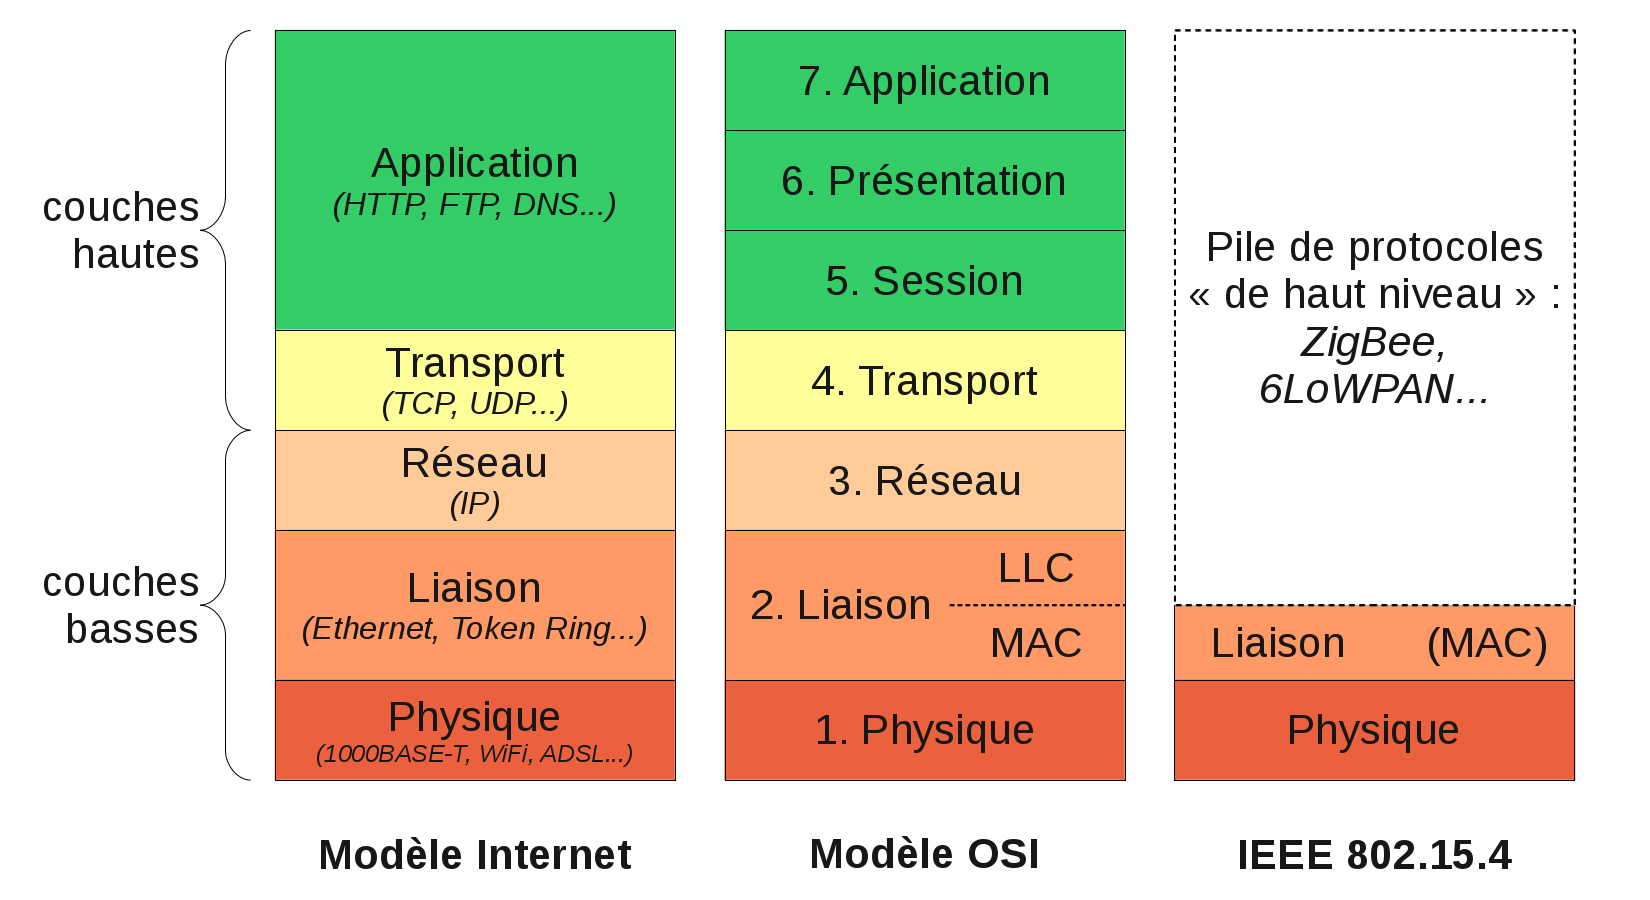
\includegraphics[width=12.5cm]{images/ch3-ip-vs-osi-vs-802154.png}
\flcaption{Comparaison entre la pile 802.15.4 et les piles OSI et Internet.}
\label{FigCompar802154IPOSI}
\end{figure}


\subsection{Couche physique}
\label{Subsec802154PHY}

La couche physique (PHY) 802.15.4 offre les fonctionnalités suivantes~:

\begin{description}

\item[Bandes de fréquences.]
De base, le standard offre trois bandes~:
une fréquence (canal) unique à 868~MHz disponible en Europe~;
une bande autour de 915~MHz offrant d'abord 10 canaux (puis étendue à 30)
disponible en Amérique du Nord~;
et la bande ISM de 2,4~GHz offrant 16 canaux et disponible dans le monde
entier.

À l'origine (2003), seule la bande à 2,4 GHz permettait d'atteindre le
débit maximal de 250~kbps, les basses fréquences (868 et 915~MHz) étaient
elles limitées à de faibles débits (20 à 40~kbps) en contrepartie d'une
portée plus grande (due à un moindre affaiblissement).
Le choix d'une bande de fréquence correspondait ainsi à un compromis entre
débit et portée, en sus d'un choix dicté par des considérations géographiques.

La révision de 2006, grâce à l'introduction de nouvelles méthodes de
modulation du signal radio, a permis aux bandes à 868 et 915~MHz d'atteindre
des débits de 100 et 250~kbps. Le choix d'une bande radio dépend donc
désormais surtout du déploiement géographique envisagé pour les réseaux
considérés.

En outre, les différents amendements ont ajouté de nouvelles bandes
de fréquences disponibles (315, 430 et 780~MHz disponibles en Chine~;
950~MHz disponible au Japon).
Ces mêmes amendements apportèrent également des méthodes de modulation
de signal supplémentaires, permettant notamment l'utilisation de bandes
à très hautes fréquences (jusqu'à 10 GHz).

L'amendement 802.15.4a a égalemement ajouté la notion d'\lang{Ultra-Wide
Band} (UWB), lequel offre, outre de plus hauts débits, la possibilité de
mesurer notamment précisément les temps de vol (c-à-d. les délais de
communication entre deux noeuds).

Les différents émetteurs~/ récepteurs radio (RF) à la norme 802.15.4 ne
peuvent pas fonctionner sur toutes les fréquences du standard~: leur choix
dépend donc de la bande de fréquences souhaitée.
Parmi les plus utilisés à l'heure actuelle, on peut par exemple citer~:
\begin{itemize}
\item La famille Texas Instruments (TI) ChipCon (CC) 1000/1100. Cette famille
regroupe des émetteurs~/ récepteurs pour les bandes à 868 et 915 MHz.
\item La famille TI CC 2400/2500, regroupant des émetteurs~/ récepteurs pour
la bande à 2,4 GHz.
\item La famille Atmel AT86RF230, regroupant également des émetteurs~/
récepteurs pour la bande à 2,4 GHz.
\end{itemize}
Nous avons au cours de nos travaux utilisé des appareils dotés de
composants radio appartenant aux deux dernières familles citées (CC2420
et AT86RF231/233), et fonctionnant donc sur la seule bande ISM à 2,4 GHz.

Notons également que l'on trouve de plus en plus fréquemment des
microcontrôleurs intégrant directement un émetteur~/ récepteur radio
dans la même puce~: par exemple, le STM32W108 de ST Microelectronics,
le SAMR21 ou la famille ATmegaRFR2 \cite{DSATmegaRFR2} d'Atmel.

\item[Mode de liaison.]
Le couche physique du standard IEEE 802.15.4 est une \emph{liaison
half-duplex}. Cela signifie que si la communication entre deux appareils
à la norme IEEE 802.15.4 est bien \emph{bidirectionnelle}~--- chaque
appareil peut assumer le rôle d'émetteur \emph{et} celui de récepteur~---
il est \emph{impossible à une seule radio au standard IEEE 802.15.4 d'émettre
et de recevoir simultanément}. La transmission d'informations entre deux
\lang{motes} dans les réseaux de capteurs sans-fil se fait donc \emph{de
façon alternée}, chaque noeud pouvant à chaque instant donné soit émettre,
soit recevoir des données~; mais jamais les deux en même temps (si le
noeud ne possède qu'un seul émetteur~/ récepteur radio).

L'un des rôles majeurs de la couche directement supérieure (MAC) est
justement de déterminer à quels instants la radio doit être en mode émission,
et à quels autres instants en réception~--- et aussi éventuellement à quels
instants elle est désactivée (pour économiser de l'énergie).

Notons que ce fonctionnement \emph{half-duplex} n'est pas propre à ce
standard 802.15.4. Le standard IEEE 802.11 (plus connu sous le nom de
\lang{``WiFi''}) est lui aussi un standard \lang{half-duplex}. Ce mode
de fonctionnement est en fait mieux adapté aux communications sans-fil,
utilisant le médium radio, lequel est par nature sujet à la diffusion,
aux variations rapides d'état et à d'autres facteurs nuisant à la qualité
de transmission. (Les réseaux câblés sont la plupart du temps en
\lang{full-duplex}, c-à-d. peuvent transmettre et recevoir simultanément,
généralement en consacrant~--- au moins~--- un fil à chaque sens
de communication.)

Ce mode de fonctionnement \lang{half-duplex} a des conséquences pratiques~:
un émetteur~/ récepteur radio doit régulièrement passer du mode émission
au mode réception et inversement. Une telle procédure n'est pas instantanée,
chaque puce radio ayant un délai de retournement indiqué dans sa
\lang{datasheet}. Le standard IEEE 802.15.4~--- dans sa version de 2011~---
indique un délai maximal pour passer du mode émission au mode réception et
inversement, que toutes les radios conformes au standard ne sont pas censées
dépasser~: constante \emph{aTurnaroundTime}, égale à 12 symboles (soit
192~$\mu$sec. pour la plupart des puces radio émettant sur la bande
de 2,4 GHz).

\item[Format de trames.]
Le standard définit un format~--- très simple~--- de trame physique
(\lang{``frame''}), dont la taille est limitée à 127 octets.
Ces 127 octets incluant les entêtes des couches supérieures (dont la
couche MAC), la taille disponible pour les données proprement dites
(charge utile ou \lang{``payload''}) est en général nettement inférieure.

\item[Modes d'adressage.]
Deux modes d'adressage complémentaires sont pris en charge~:
\begin{itemize}
\item un adressage court sur 16~bits (plus un identifiant de réseau~---
identifiant PAN~--- de 16~bits également) dont l'intérêt est de limiter
la taille des entêtes de trames~;
\item un adressage long (dit <<~adressage IEEE~>>) sur 64~bits permettant
\lang{a priori} directement une identification unique de chaque appareil.
\end{itemize}

\item[Détection du médium.]
Le standard inclut la détection d'énergie (ED~: \lang{Energy Detection})
sur le médium radio, et par extension la vérification de la disponibilité
du canal radio (CCA~: \lang{Clear Channel Assessment}).

\item[Qualité de service.]
Le standard prend en charge la définition et l'indication de la qualité
de liaison (LQI~: \lang{Link Quality Indicator}) pour une transmission
de trame donnée. Le RSSI (\lang{Received Signal Strength Indicator}),
s'il n'est quévoqué dans le glossaire du standard 802.15.4, est également
la plupart du temps pris en charge au niveau physique (émetteurs~/
récepteurs radio).

\end{description}

Toutes ces propriétés sont implantées de façon matérielle par les
différents émetteurs~/ récepteurs radio conformes au standard 802.15.4~---
qu'il s'agisse de composants autonomes, ou de circuits intégrés à des
microcontrôleurs ou \lang{System-on-Chip} (SoC).

La couche PHY, au niveau logiciel, notamment dans un système d'exploitation
spécialisé, consiste donc en un jeu de primitives (implantées dans des
pilotes) permettant d'exploiter ces émetteurs~/ récepteurs radio. On peut
envisager cette couche comme une couche d'abstraction matérielle
(HAL~: \lang{Hardware Abstraction Layer}) vis-à-vis de la couche MAC
et des couches supérieures de la pile réseau du système.


\subsection{Couche MAC}
\label{Subsec802154MAC}

Située immédiatement au-dessus de la couche physique, la couche MAC
du standard 802.15.4 repose sur la méthode CSMA/CA (\lang{Carrier Sense
Multiple Access with Collision Avoidance}). Une version différente de
cette technologie est déjà utilisée (sous le même nom) dans le standard
IEEE 802.11 (alias \lang{``WiFi''}).

La couche MAC standard peut utiliser cette méthode selon deux modalités
différentes, selon l'utilisation ou non de \lang{``beacons''} (ou balises
\footnotemark[1]) pour synchroniser les différents noeuds et identifier
les différents réseaux (PAN). Sans \lang{``beacons''}, la couche MAC
standard emploie toujours des cycles de fonctionnement (\lang{``duty
cycles''}) fixes, sans prendre en compte l'utilisation réelle du réseau
et le débit des données transmises. Le mode <<~avec \lang{beacons}~>>
permet d'ajuster certains paramètres de fonctionnement \cite{TheseSKhssibi}.
Certains éléments restent toutefois immuables, même dans ce mode (par
exemple les 16 \lang{slots} de temps dans la \lang{superframe}).

\footnotetext[1]{Pour des raisons pratiques, nous emploierons dans la suite
de ce manuscrit le terme anglo-saxon \lang{``beacon''}, plus utilisé dans
la littérature.}

Le standard 802.15.4 est à la base conçu pour faire fonctionner des réseaux
ayant une topologie en étoile~; pour cela, le standard permet de
différencier les noeuds en deux types~:

\begin{itemize}

\item les noeuds à fonctionnalités complètes (FFD~: \lang{Full Function
Devices}), capables de jouer aussi bien le rôle de <<~noeud simple~>>
occupant une des extrêmités du réseau, que celui plus évolué de coordinateur
de réseau (en mode <<~avec \lang{beacons}~>>)~;

\item les noeuds à fonctionnalités réduites (RFD~: \lang{Reduced Function
Devices}), limités au rôle de <<~noeuds simples~>>

\end{itemize}

Dans notre terminologie, un <<~noeud simple~>> est un noeud dont la
défaillance ne met pas en péril le fonctionnement de l'ensemble,
au contraire d'un routeur ou d'un coordinateur dont la seule panne
entraîne la perte de tout un réseau.

Un exemple de base d'un schéma topologique d'un réseau de capteurs
sans-fil (WSN) est montré figure \vref{FigTopoWSN}. Celui présenté
ici est composé de quatre sous-réseaux (PAN) différents, possédant chacun
un routeur jouant également le rôle de coordinateur de son PAN. Les noeuds
simples (<<~feuilles~>> de l'arborescence) ne communiquent qu'avec leur
propre coordinateur, ces derniers se chargeant de transmettre les données
de PAN en PAN de façon adéquate.

\begin{figure}[!hbt]
\centering
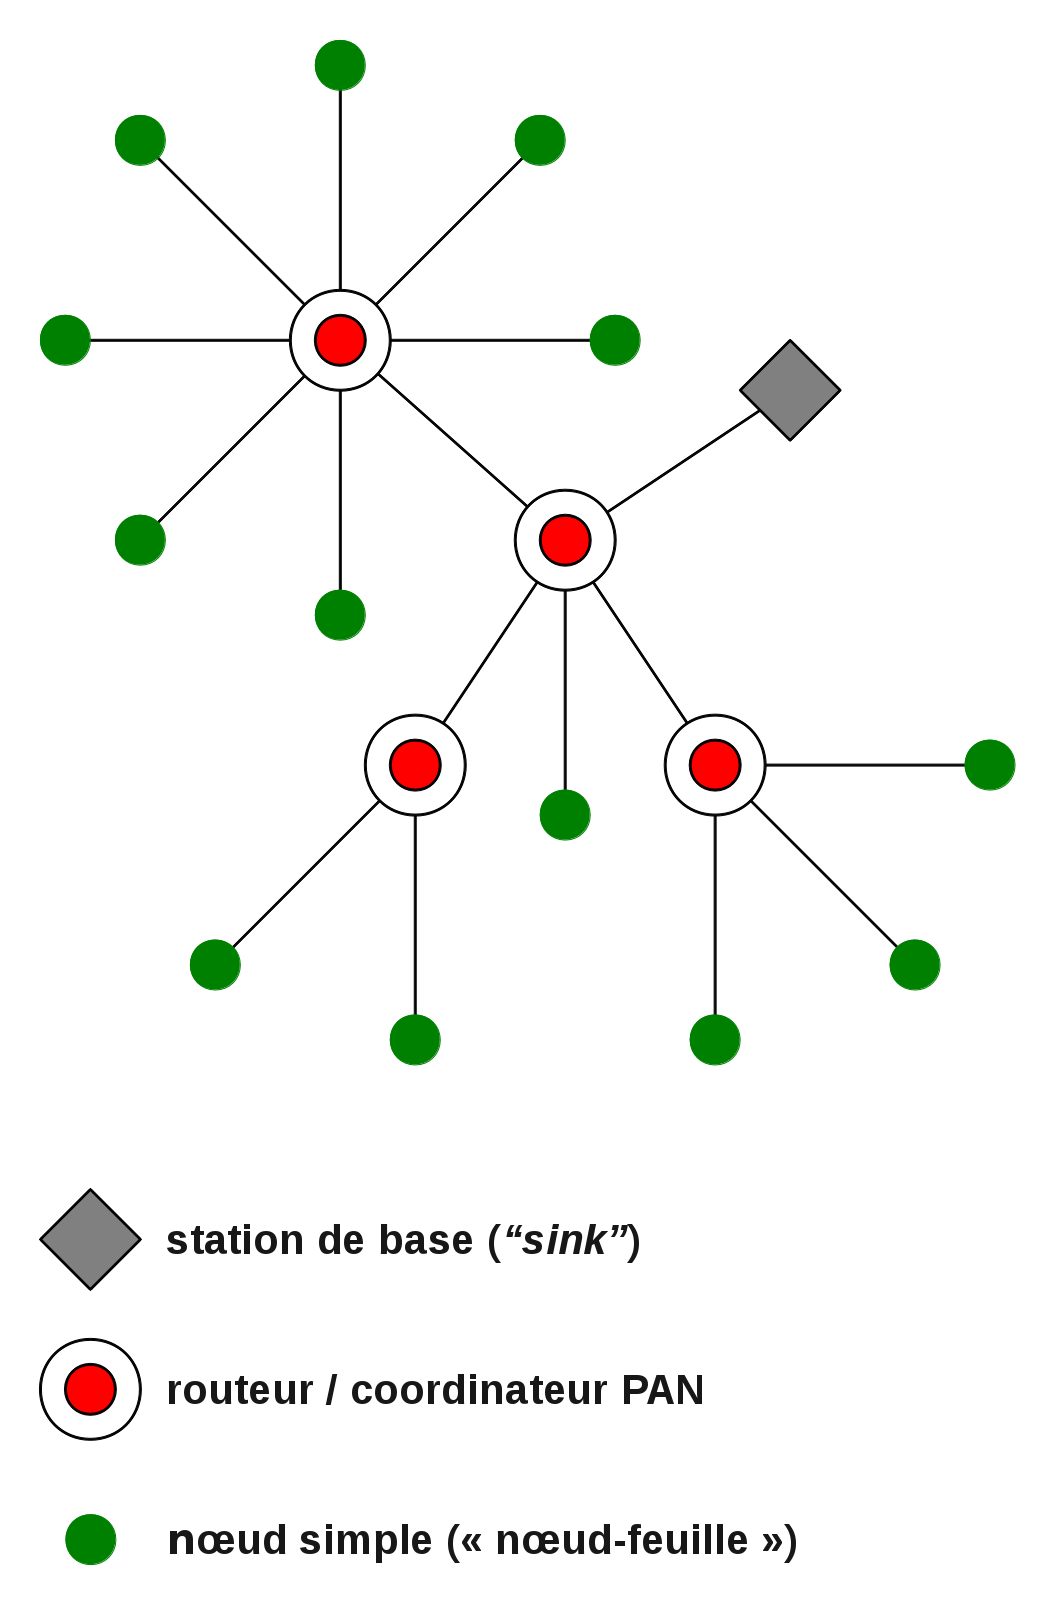
\includegraphics[width=7cm]{images/ch3-topo-wsn.png}
\flcaption{Schéma topologique d'un réseau de capteurs sans-fil (WSN).
(D'après \cite{coursEnsem})}
\label{FigTopoWSN}
\end{figure}

Ces réseaux (PAN) peuvent eux-mêmes être reliés entre eux de façon maillée
et/ou arborescente (selon les protocoles de routage utilisés par dessus
802.15.4).

\subsubsection{CSMA/CA}
\label{ParCSMACA}

Cette méthode consiste à éviter les collisions potentielles sur le médium
en vérifiant préalablement la disponibilité du canal radio et, en cas
d'encombrement, en attendant pendant un délai aléatoire avant de retenter
une écoute.

Plus précisément, l'implantation de CSMA/CA dans le standard 802.15.4
en version de base <<~non slottée~>> est la suivante~:

\begin{enumerate}

\item un noeud souhaitant émettre une trame doit d'abord attendre pendant
un délai dont la durée est \emph{aléatoirement} choisie entre 0 et
$2^{BE} - 1$ unités de temps nommées \nom{BP} (\lang{``Backoff Period''})~.
La valeur d'une BP est une constante dépendant de la bande choisie pour
la couche physique (elle vaut 320~microsecondes pour la bande ISM à 2,4 GHz).
La valeur $BE$ est nommée \lang{``Backoff Exponent''}, et est initialisée
à une valeur définie dans le standard sous le nom de \emph{macMinBE}
(3 par défaut).

\item une procédure de CCA est alors effectuée~: le CCA consiste à écouter
le medium radio durant un délai spécifique~--- nommé DIFS
(\lang{Distributed Inter-Frame Space})~---, si le medium reste libre
pendant ce délai, le noeud peut alors émettre sa trame~; 

\item si le médium radio est encombré, on revient à la première étape
d'attente d'un délai aléatoire, en ayant toutefois incrémenté la valeur
de BE, dans la limite de la valeur maximale \emph{macMaxBE} définie
par le standard (5 par défaut). Toutefois, au bout d'un nombre maximal
d'essais, défini par le standard sous le nom de \emph{macMaxCSMABackoffs}
(4 par défaut), l'envoi de la trame est considéré comme échoué par la
couche MAC.

\end{enumerate}

La méthode CSMA/CA peut également fonctionner en mode <<~slotté~>>, de
façon à s'adapter aux protocoles MAC où les transmissions doivent se caler
sur des intervalles de temps (\lang{``slots''}) bien définis. Dans ce cas,
un nouveau paramètre, nommé \lang{``Contention Window''} (\emph{CW})
intervient pour s'assurer que le médium radio a été détecté libre (CCA)
un certain nombre de fois avant de commencer une émission~; cette étape
supplémentaire a notamment pour but de faciliter la transmission des
messages d'acquittement signalant la bonne réception d'une trame (ACK).
Par défaut, le standard fixe la valeur initiale de $CW$ ($CW_0$) à 2.

L'organigramme décrivant le fonctionnement de la méthode CSMA/CA est
schématisé dans la figure \vref{FigOrganigrammeCSMACA}.
Dans cette figure, la branche de gauche présente la version <<~slottée~>>,
employée notamment dans le mode \lang{``beacon''} du protocole MAC du
standard IEEE 802.15.4~; tandis que la branche de droite présente la
version simple <<~non slottée~>> qui est en général utilisée pour les
protocoles non synchronisés (tels que LPL, LPP, cf. suite du chapitre).

\begin{figure}[!pthb]
\centering
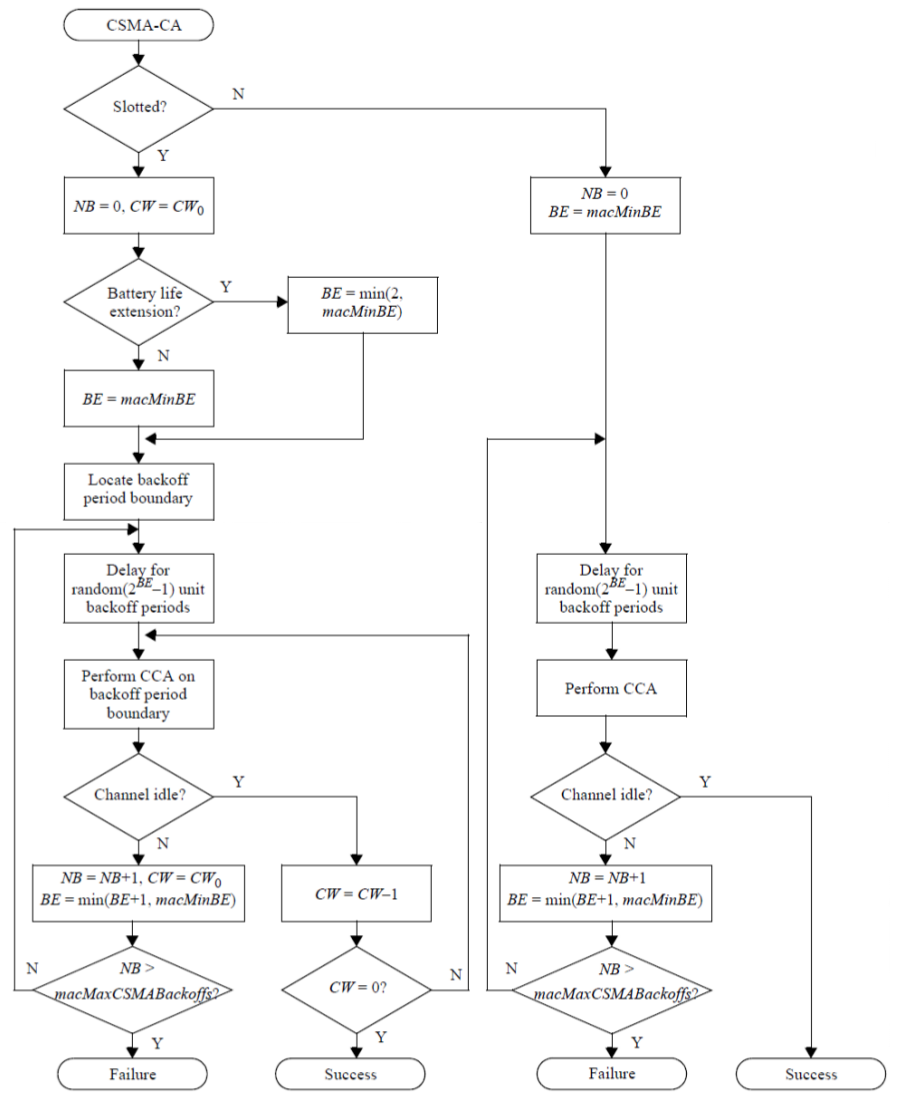
\includegraphics[width=14.25cm]{images/ch3-csma-ca-std.png}
\flcaption{Organigramme de l'algorithme de la m\'ethode CSMA/CA.
(Source~: \cite{IEEE802154-2011}, figure 11)}
\label{FigOrganigrammeCSMACA}
\end{figure}

En sus de la méthode CSMA/CA, notons qu'il existe également un mécanisme
obligatoire d'acquittement des trames. Ainsi, à la réception de chaque
trame de données, le noeud de destination doit renvoyer un acquittement
à l'envoyeur~; si après envoi d'une trame de données, le noeud émetteur
ne reçoit pas d'acquittement dans un délai voulu (\lang{``timeout''}),
l'envoi de la trame est considéré comme un échec.

\subsubsection{Mode \lang{``non-beacon''}}
\label{Par802154MACSimple}

Le mode de fonctionnement le plus simple de la couche MAC du standard
802.15.4 repose exclusivement sur l'emploi de la méthode CSMA/CA <<~non
slottée~>> décrite section \vref{ParCSMACA}. Il n'y a aucune notion de cycle
de fonctionnement~: le coordinateur est constammant en fonctionnement
(la plupart du temps en écoute), tandis que les noeuds simples n'accèdent
au médium radio que lorsqu'ils ont besoin d'envoyer ou recevoir des données.

La réception de données s'effectue grâce à un bit nommé \lang{``Frame
Pending''} de l'entête MAC 802.15.4, via lequel le coordinateur indique
à un de ses noeuds-feuilles qu'il attend de lui envoyer une trame lui
étant destinée. Le noeud destinataire peut alors envoyer une trame
spéciale dite <<~de commande~>> (\lang{``Data Request''}) pour déclencher
la réception proprement dite.

Ce mode est bien adapté aux réseaux dans lesquels les noeuds simples
émettent des données de façon sporadique (c'est-à-dire passent la
quasi-totalité de leur temps en <<~sommeil~>>), et où les données transmises
n'ont pas un caractère urgent (ce mode sans \lang{``beacon''} n'offrant
aucune garantie d'accès au canal pour une période donnée).

Il est ainsi possible d'avoir des noeuds simples fonctionnant sur une
batterie dont l'autonomie pourra être longue. Par contre, le noeud central
jouant le rôle de coordinateur doit lui être constamment à l'écoute, ce qui
impose la contrainte de le faire fonctionner sur une source d'énergie
constante (secteur).

\subsubsection{Mode \lang{``beacon''} (ou mode balisé)}
\label{Par802154MACBeacon}

Le second mode de fonctionnement de la couche MAC standard impose au
noeud central, jouant le rôle de coordinateur de PAN (compatible avec
celui de routeur, ce qui représente l'immense majorité des cas), l'envoi
régulier de \lang{``beacons''} à chaque début de cycle de fonctionnement
(\lang{``duty cycle''}).

Ces \lang{``beacons''} servent à synchroniser les différents noeuds du PAN
(ainsi qu'à identifier ce dernier).

Dans ce mode, un cycle de la couche se décompose en~:
\begin{description}
\item[l'envoi d'un \lang{``beacon''}] par le noeud coordinateur du PAN, cet
envoi n'utilisant pas la méthode CSMA/CA, mais la diffusion directe à tous
les noeuds à l'écoute (\lang{``broadcast''}), aucun autre noeud n'étant
en effet censé être autorisé à émettre spontanément hors cycle~;
le \lang{``beacon''} est, dans ce mode, en général la trame comportant
le fameux bit \lang{``Frame Pending''} pour permettre l'envoi de
données aux noeuds-feuilles~;
\item[une CAP] (\lang{Contention Access Period}) période durant laquelle
les noeuds simples émettent vers le noeud central, ou recoivent les données
leur étant destinées depuis celui-ci, en mode CSMA/CA~;
\item[une CFP] (\lang{Contention Free Period}) période durant laquelle
il est possible de garantir l'accès au médium radio pour un noeud (ou
plusieurs noeuds consécutifs)~;
\item[une période de sommeil] durant laquelle le PAN est mis en inactivité
ce qui permet aux différents noeuds, y compris le noeud central, de
désactiver leur émetteur~/ récepteur radio pour économiser leur énergie.
\end{description}

L'ensemble constitué par la CAP et la CFP d'un cycle donné constitue
la \nom{supertrame} (en anglais \lang{``superframe''}, par opposition
à la periode de sommeil).

Le cycle de fonctionnement du protocole MAC standard 802.15.4 en mode
\lang{``beacon''} est représenté dans la figure
\vref{FigMAC802154beacon}.

\begin{figure}[!hbt]
\centering
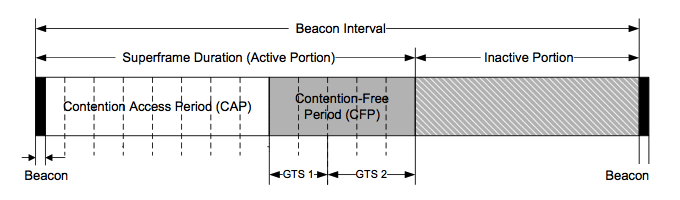
\includegraphics[width=12.5cm]{images/ch3-ieee802154-mode-beacon.png}
\flcaption{Cycle de fonctionnement du protocole MAC du standard IEEE
802.15.4 en mode \lang{``beacon''}.
(Source~: \cite{Evolution-MAC-WSN-Survey-2013})}
\label{FigMAC802154beacon}
\end{figure}

Cette supertrame est divisée en 16 \lang{``time slots''}, lequels sont
répartis entre CAP et CFP par le noeud coordinateur à chaque nouveau cycle,
en fonction des besoins du trafic réseau. Les \lang{``time slots''} alloués
à la CFP sont nommés \nom{GTS} (\lang{Guaranteed Time Slots})~; le standard
définit la procédure permettant à un noeud simple de demander au noeud
coordinateur de PAN de lui allouer un ou plusieurs GTS au cycle suivant.

On voit ainsi que ce mode offre plusieurs avantages par rapport au mode
\lang{``non-beacon''}~:
\begin{itemize}
\item le noeud coordinateur peut établir à lui seul son réseau (PAN)~;
\item la présence d'une CFP permet de prévoir l'envoi de données
importantes, dont le transport nécessite un accès garanti au médium
radio sans risque de collision~;
\item la CFP permet également d'envisager l'envoi de lots de trames
successifs (pour la transmission de données de grande taille), de façon
plus robuste que par l'utilisation de la méthode CSMA/CA.
\end{itemize}

On voit que la division de la période d'activité (\lang{superframe}) en CAP
et CFP est un moyen d'adapter le fonctionnement de la couche MAC au trafic
sur le médium radio. Par défaut, cette adaptabilité est limitée par le fait
que la durée d'un cycle, de la \lang{superframe}, et donc le rapport entre
ces deux durées, sont des constantes fixées lors de la configuration du PAN.
Des travaux ont récemment été menés pour adapter dynamiquement ces
paramètres au trafic réseau \cite{TheseSKhssibi}, le standard ne le
prévoyant pas, mais ne l'interdisant pas non plus.

\subsubsection{802.15.4e}
\label{Par802154e}

Le standard IEEE 802.15.4 continue à évoluer, et les groupes de travail
dédiés de l'IEEE ne cessent de le réviser et de le compléter~--- via
des amendements~--- au cours du temps.

Les amendements 802.15.4a, 4b, 4c et 4d ont successivement amené de
nouvelles bandes de fréquences et méthodes d'encodage du signal radio,
l'amendement IEEE 802.15.4a ayant notamment amené la notion d'UWB,
comme dit plus haut en section \vref{Subsec802154PHY}

Un amendement récent au standard, l'amendement 802.15.4e, adopté en 2012,
a ajouté une nouvelle couche MAC nettement plus complexe, incluant
notamment des mécanismes de multiplexage temporel \emph{et} fréquentiel
des transmissions radio. Nous reviendrons sur cet amendement 802.15.4e
dans la section \vref{SubsecProtoMACFDMA} consacrée aux protocoles MAC
multicanaux.


%%%%%%%%%%%%%%%%%%%%%%%%%%%%%%%%%%%%%%%%%%%%%%%%%%%%%%%%%%%%%%%%%%%%%%%%%%%%%

\section{Protocoles MAC}
\label{SecProtoMAC}

Outre les couches MAC <<~officielles~>> proposées par le standard
802.15.4, la communauté scientifique a proposé de nombreux protocoles
alternatifs destinés à surpasser les limitations du
protocole standard, notamment sa version simple reposant sur la seule
méthode CSMA/CA.

Contrairement au mode simple, et de façon similaire au mode balisé décrit
section \vref{Par802154MACBeacon}, ces protocoles MAC alternatifs
reposent sur la notion de \lang{``duty cycle''}. Toute la difficulté pour
la mise au point de ces protocoles consiste donc à fixer des \emph{points
de rendez-vous} entre les différentes noeuds pour assurer correctement
leur synchronisation.

On peut ainsi diviser ces divers protocoles en différentes familles, selon
les méthodes utilisées pour fixer ces points de rendez-vous~:

\begin{itemize}

\item les protocoles MAC synchrones, employant des mécanismes de
synchronisation explicites entre noeuds pour la transmission de trames~:
S-MAC et T-MAC en sont deux exemples~;

\item les protocoles MAC asynchrones basés sur l'écoute à basse énergie
(LPL~: \lang{Low Power Listening})~: B-MAC, X-MAC et ContikiMAC en sont
trois exemples (ce dernier étant aujourd'hui très largement utilisé)~;

\item les protocoles MAC asynchrones basés sur l'émission à basse énergie
(LPP~: \lang{Low Power Probing})~: RI-MAC en étant l'exemple le plus connu~;

\item les protocoles MAC basés sur l'ordonnancement temporel~: LMAC,
AI-LMAC en sont deux exemples~;

\item les protocoles MAC multicanaux~: différents protocoles ont exploré
cette voie, mais surtout, l'extension du standard IEEE 802.15.4e fait
désormais appel au multiplexage fréquentiel des transmissions, via un
mécanisme nommé TCSH.

\end{itemize}

Nous allons dans cette section étudier ces différents types de protocoles
de façon consécutive, à chaque fois en se penchant sur un ou deux
protocoles représentatifs de chaque famille (notre but n'étant ici
encore pas d'être exhaustif).

Enfin, nous étudierons plus en détail plusieurs protocoles MAC avancés~:
la famille CoSenS et iQueue-MAC, conçus et développés au sein du LORIA
et de l'INRIA Nancy, sur lequels nous avons focalisé nos travaux.

La présente section \ref{SecProtoMAC} reprend la présentation effectuée dans
les supports de cours de Y.-Q. Song sur les systèmes communicants contraints
\cite{coursEnsem}, ainsi que des données présentées dans l'article de
référence (\lang{``survey''}) de P. Huang, L. Xiao et al
\cite{Evolution-MAC-WSN-Survey-2013} et la thèse de B. Nefzi
\cite{TheseBNefzi}.


\subsection{Protocoles MAC synchrones}
\label{SubsecProtoMACSynchrones}

Cette famille de protocoles MAC est basée sur la synchronisation explicite
des cycles de fonctionnement de noeuds voisins. Il s'agit de la solution
la plus évidente pour permettre la communication entre appareils, mais
cela implique des coûts supplémentaires (en temps et en complexité)
pour effectuer cette synchronisation. Ce type de protocoles n'ayant
pas de difficultés pour établir des communications entre noeuds,
ils peuvent faire l'objet d'optimisations pour augmenter le débit
de données et réduire les délais de transmission.

\subsubsection{S-MAC}
\label{ParSMAC}

Un premier exemple de protocole synchrone est le protocole S-MAC \cite{SMAC}.
Celui-ci est basé sur la méthode CSMA/CA complétée par l'envoi de signaux
indiquant qu'un noeud a des données à envoyer (RTS~: \lang{Ready To Send})
et qu'un noeud est prêt à recevoir (CTS~: \lang{Clear To Send}). Ce mode
de fonctionnement est celui utilisé par le standard 802.11 (``Wi-Fi'').

Un cycle de fonctionnement sous le protocole S-MAC est divisé en une
période active et une période inactive. La période active est la seule
pendant laquelle un noeud peut envoyer et recevoir des données, la période
inactive correspondant à la désactivation de l'émetteur~/ récepteur radio
pour économiser l'énergie. La période active est elle-même divisée en
une période de synchronisation, et une période d'échange de données.

Dans ce protocole, chaque noeud choisit ses périodes actives et inactives
en fonction de ses voisins. Le premier noeud à démarrer est le seul
choisissant librement ses périodes, et annonce ensuite régulièrement
ses périodes par l'envoi de signaux de synchronisation (SYNC) durant
une période dédiée (au début de la période active). Les noeuds démarrant
ensuite vont alors adapter leurs propres périodes sur celles annoncées
par les noeuds précédents. Ce mécanisme d'adaptation porte le nom
\lang{``d'adaptative listening''}.

\begin{figure}[!hbt]
\centering
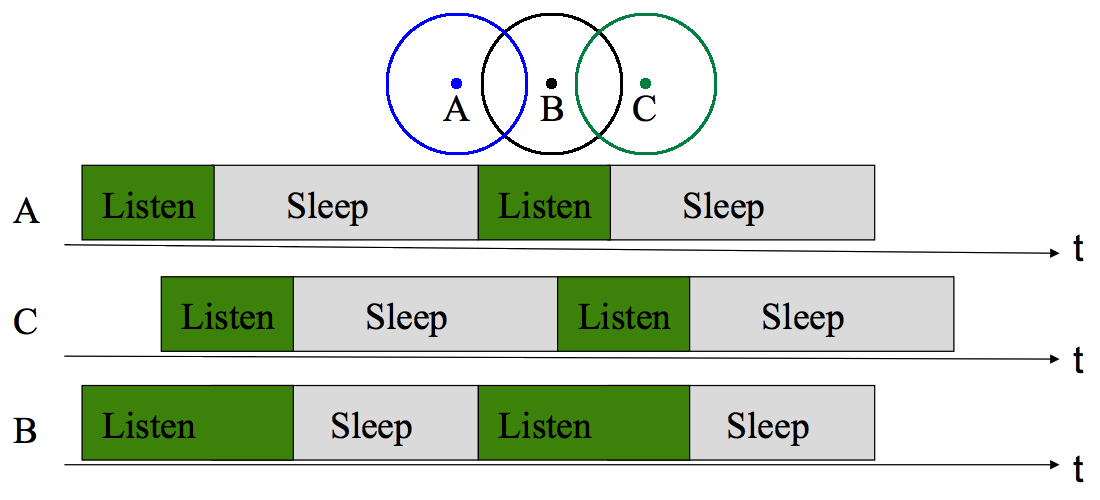
\includegraphics[width=12.5cm]{images/ch3-s-mac.png}
\flcaption{\lang{Adaptative listening} entre trois noeuds suivant
le protocole S-MAC.
(Source~: \cite{coursEnsem})}
\label{FigSMACadapt}
\end{figure}

La figure \vref{FigSMACadapt} montre un exemple de synchronisation
entre plusieurs noeuds sous S-MAC. Le noeud B, démarrant en dernier, adapte
sa période active à celle de ses deux voisins A et C. A et C étant hors de
portée l'un de l'autre, ne vont par contre pas se synchroniser entre eux.

Ce protocole est donc basé sur la définition de rendez-vous entre
émetteur et récepteur. L'utilisation de nombreux signaux pour coordonner
les transmissions (SYNC, RTS, CTS) entraîne un surcoût (\lang{``overhead''})
élevé diminuant d'autant la bande passante disponible pour les données,
même si S-MAC est capable d'envoyer des trames par lots (\lang{``send
burst''}), après une seule séquence RTS/CTS, pour accélérer le traitement
de données volumineuses.

Ce protocole ayant des cycles de fonctionnement fixes et un mécanisme
de synchronisation assez lourd, son adaptabilité au trafic sur le réseau
est très faible.

Notons enfin que toute synchronisation entre appareils différents est
susceptible d'être victime du phénomène de dérive des horloges (dû aux
inévitables différences de fonctionnement entre les horloges internes
de chaque appareil). S-MAC utilisant des périodes actives assez longues,
il est peu sensible aux perturbations dues à ce phénomène. 

\subsubsection{T-MAC}
\label{ParTMAC}

Le protocole T-MAC \cite{TMAC} est une amélioration de S-MAC. Dans T-MAC,
la durée de la période active n'est plus fixée à l'avance, mais chaque
noeud reste éveillé jusqu'à ce qu'aucun signal ne le concernant n'ait
été entendu pendant un certain délai (notion de \lang{``timeout''}).
Ce schéma permet un meilleure adaptabilité au trafic réseau, en permettant
notamment une période de sommeil plus longue en cas de faible trafic,
d'où une meilleure économie d'énergie. La figure \vref{FigSMACvsTMAC}
permet de comparer le fonctionnement de base des protocoles S-MAC et T-MAC.
On notera que ce dernier adapte sa période d'éveil à l'intensité du trafic
réseau.

\begin{figure}[!hbt]
\centering
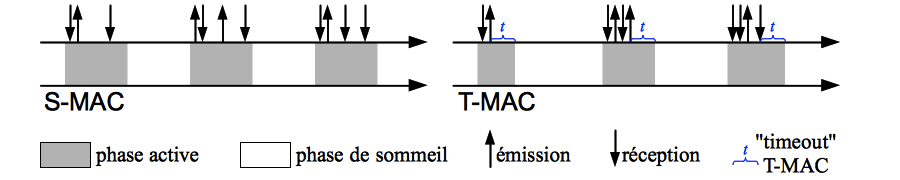
\includegraphics[width=12.5cm]{images/ch3-s-mac-vs-t-mac.png}
\flcaption{Comparaison du fonctionnement de S-MAC et T-MAC.
(Source~: \cite{coursEnsem})}
\label{FigSMACvsTMAC}
\end{figure}

T-MAC reprend également la capacité de S-MAC à effectuer des envois
de trames par lots (après une unique paire de signaux RTS/CTS) pour
un traitement plus efficace des données volumineuses.


\subsection{Protocoles MAC asynchrones LPL}
\label{SubsecProtoMACLPL}

Dans un protocole MAC asynchrone, chaque noeud garde sa propre base de temps
autonome. L'absence de synchronisation entre noeuds voisins permet (en
théorie) d'éviter d'employer des phases de synchronisation systématiques à
chaque cycle, donc à chaque appareil d'avoir un \lang{``duty cycle''} plus
réduit, et ainsi d'économiser son énergie, mais rend plus délicat
l'établissement de communications entre noeuds. Toute la difficulté
dans la mise au point d'un protocole asynchrone est de trouver une méthode
efficace en ce sens.

La famille des protocoles dits LPL (\lang{``Low Power Listening''}, ou
écoute à faible puissance) repose sur le principe suivant~: chaque noeud
passe la quasi-totalité de son temps en sommeil, c'est-à-dire avec sa radio
désactivée~; pour déterminer si un message lui est destiné, il va de façon
cyclique activer sa radio et vérifier si le canal radio est occupé
(la procédure consistant à écouter le médium radio pour vérifier s'il est
libre est appelée CCA~: \lang{Clear Channel Assessment}).

Les protocoles LPL vont différer sur la méthode d'envoi des données par les
noeuds émetteurs~: il s'agit en effet de s'assurer que le noeud destinataire
remarquera qu'une transmission lui est destinée~--- et donc d'entrer en
contact avec ce dernier lorsqu'il effectue son CCA~--- tout en essayant
de minimiser l'énergie consommée par le noeud émetteur (en limitant le
temps où la radio de ce dernier doit émettre).

\subsubsection{B-MAC}
\label{ParBMAC}

Un premier exemple de protocole LPL est B-MAC (Berkeley MAC) \cite{BMAC}.
Dans ce protocole, un noeud devant envoyer des données émet un très long
préambule (une trame ne contenant aucune donnée utile et ne servant qu'à
signaler une future émission de données). Ce préambule est très long car
son émission doit durer plus longtemps que l'intervalle entre deux CCAs
consécutifs du récepteur. De plus, ce préambule ayant une taille fixe,
le récepteur devra, lorsqu'il l'aura détecté, attendre sa fin avant de
pouvoir recevoir ses données proprement dites. Ce mode de fonctionnement
est représenté dans la figure \vref{FigBMAC}.

\begin{figure}[!hbt]
\centering
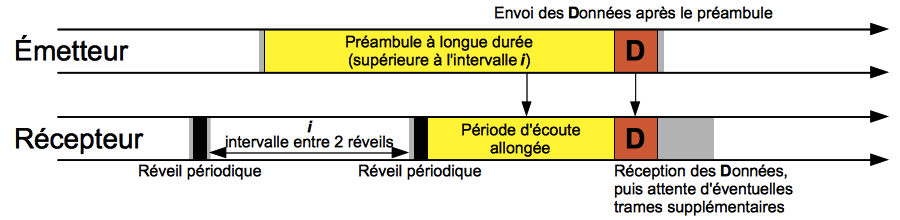
\includegraphics[width=12.5cm]{images/ch3-b-mac.png}
\flcaption{Schéma de fonctionnement de B-MAC (protocole LPL typique).
(Source~: \cite{coursEnsem})}
\label{FigBMAC}
\end{figure}

On voit que cette procédure entraîne une dépense d'énergie maximale pour
le noeud émetteur (à cause de la nécessité d'envoyer ce très long préambule)
ainsi qu'un encombrement important du canal radio, augmentant le risque
de collisions. La taille fixe du préambule comme de l'intervalle entre CCAs
consécutifs rend également le protocole très peu adaptable au trafic réseau.

\subsubsection{WiseMAC}
\label{ParWiseMAC}

Notre second exemple de protocole LPL, nommé WiseMAC \cite{WiseMAC},
emploie une technique consistant à <<~apprendre~>> les cycles de
fonctionnement des noeuds voisins d'un même PAN. Pour ce faire, ce
protocole repose d'abord sur l'envoi de longs préambules (comme B-MAC),
auquels les noeuds récepteurs du PAN répondent par un acquittement lors
de leur phase cyclique de réveil (\lang{``channel sampling''}).
Une fois les cycles de tous les noeuds du PAN connus, WiseMAC se distingue
alors de B-MAC, en recourant à l'envoi de préambules bien plus courts,
ce qui est possible en démarrant les transmissions au moment adéquat
(en incluant une certaine marge de sécurité pour éviter les problèmes
dûs à la dérive des horloges entre appareils). La possibilité, après
un temps d'apprentissage, d'utiliser des préambules raccourcis améliore
considérablement la consommation d'énergie des différents noeuds~---
aussi bien des émetteurs ayant moins de temps à passer à émettre, que
des récepteurs n'ayant plus à écouter inutilement des préambules trop
longs~--- et optimise l'utilisation du médium radio en le libérant
pour la transmission de données <<~utiles~>>, augmentant ainsi le
débit maximal utile réel du réseau.

\subsubsection{X-MAC}
\label{ParXMAC}

Notre troisième exemple de protocole LPL, X-MAC \cite{XMAC}, optimise
nettement la procédure d'envoi, en remplaçant les long préambules de B-MAC
par de très courts trames-préambules intégrant en outre l'adresse du
noeud destinataire, comme on peut le voir dans la figure \vref{FigXMAC}.
Cette technique améliore non seulement la dépense d'énergie par le noeud
émetteur ainsi que le taux d'occupation du médium, mais permet également
d'éviter de garder inutilement éveillés des noeuds tiers, le destinataire
d'une future émission étant clairement identifié par ces courts préambules.
Enfin, X-MAC inclut également l'envoi d'un acquittement préalable par le
noeud récepteur (assimilable à un signal CTS) avant l'envoi des données
proprement dites. 

\begin{figure}[!hbt]
\centering
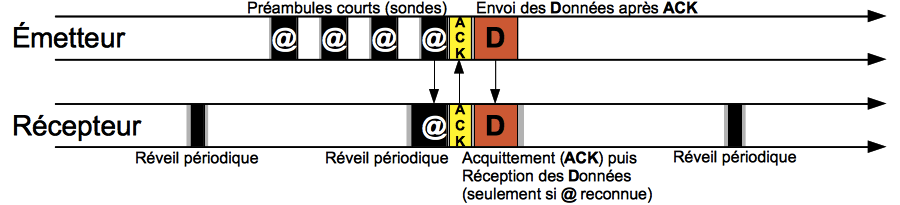
\includegraphics[width=12.5cm]{images/ch3-x-mac.png}
\flcaption{Schéma de fonctionnement du protocole X-MAC.
(Source~: \cite{coursEnsem})}
\label{FigXMAC}
\end{figure}

\subsubsection{ContikiMAC}
\label{ParContikiMAC}

Notre quatrième exemple de protocole LPL est ContikiMAC \cite{ContikiMAC}.
Celui-ci est nettement plus récent que les précédents, et a été conçu
spécifiquement pour fonctionner sous Contiki OS (système que nous
présenterons dans la section \vref{SubsecContikiOS}).

Ce protocole, par rapport à X-MAC, simplifie encore la procédure d'envoi
des données, en supprimant totalement la notion de préambule~: lors d'une
transmission, c'est désormais la trame de données elle-même qui est
émise de façon répétitive, jusqu'au prochain réveil du noeud récepteur.
Une fois la trame de données bien reçue, le destinataire envoie un
acquittement (ACK standard 802.15.4) pour mettre fin à l'émission de la
trame. Le fonctionnement de ContikiMAC est représenté
dans la figure \vref{FigContikiMAC}.

\begin{figure}[!hbt]
\centering
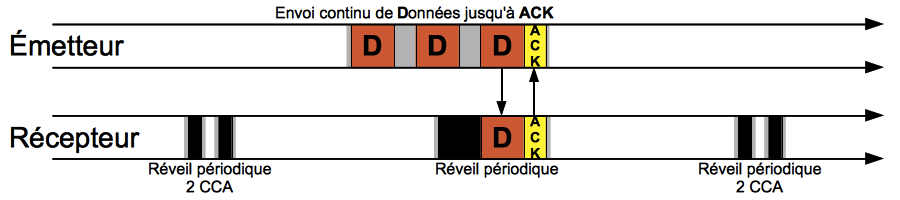
\includegraphics[width=12.5cm]{images/ch3-contikimac.png}
\flcaption{Schéma de fonctionnement du protocole ContikiMAC.
(Source~: \cite{coursEnsem})}
\label{FigContikiMAC}
\end{figure}

Autre particularité~: chaque noeud effectue \emph{deux} CCA à chaque réveil
cyclique, et ne retombe en sommeil que si ces deux CCA ont indiqué
la non-occupation du canal radio. (Ces deux CCA, séparés par un délai
calculé à partir du délai standard entre émission de trames (DIFS)
et la taille minimale d'une trame 802.15.4, permettent de consommer
moins d'énergie qu'une longue écoute. Ces deux CCA ont ainsi la durée
minimale nécessaire pour déterminer ou non l'occupation du médium radio.)

Enfin, signalons que les versions récentes de ContikiMAC bénéficient d'une
optimisation supplémentaire~: après un envoi réussi, le noeud émetteur
mémorise la période de réveil du destinataire, afin d'envoyer les
trames suivants au meilleur moment et ainsi limiter au maximum
les transmissions inutiles. Cette optimisation est nommée \lang{``phase
lock''} par les concepteurs de ContikiMAC. \\
On peut rapprocher cette technique de \lang{``phase lock''} du mécanisme
d'apprentissage des cycles des noeuds observé antérieurement dans le
protocole WiseMAC.


\subsection{Protocoles MAC asynchrones LPP}
\label{SubsecProtoMACLPP}

Si les protocoles LPL sont conçus pour avoir une meilleure adaptabilité
au trafic que les protocoles synchrones (comme S-MAC ou T-MAC),
ils souffrent néanmoins de plusieurs inconvénients~:
\begin{itemize}
\item une efficacité energétique non optimale~: B-MAC, avec ses très longs
préambules, est clairement insuffisant dans ce domaine~;
\item l'envoi de préambules (ou de trames dans le cas de ContikiMAC)
avant la <<~transmission réelle~>> occupe inutilement le medium,
augmentant ainsi les délais de transmission, les risques de collision,
et diminuant le débit réel maximal du trafic~;
\item l'inadéquation aux trafics élevés~--- par exemple lors de <<~pics~>>
ou <<~pointes~>> de transmissions~--- à cause de la méthode CSMA/CA
sous-jacente~;
\item la risque de <<~collisions cachées~>> entre noeuds~: ce terme
regroupe les cas où plusieurs paires de noeuds émetteurs/récepteurs,
ayant chacune indépendemment des données à se transmettre, se gênent
mutuellement si elles sont partiellement à portée l'une de l'autre.
La figure \vref{FigCollisionsCachees} illustre la survenue
d'un de ces problèmes~: les deux récepteurs sont à portée des deux
émetteurs, ces derniers étant par contre incapables de se détecter
mutuellement, ce qui provoque une collision entre les trames transmises
par chacun des deux émetteurs.
\end{itemize}

\begin{figure}[!hbt]
\centering
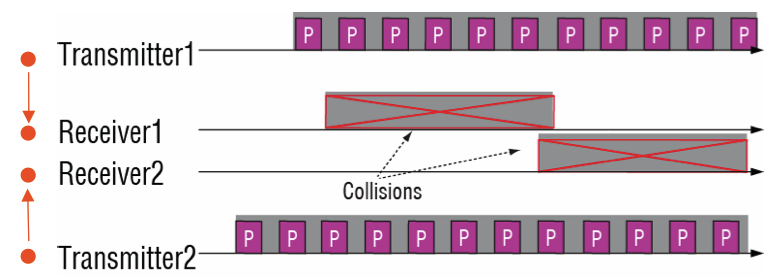
\includegraphics[width=12.5cm]{images/ch3-collisions-cachees.png}
\flcaption{Survenue d'une <<~collision cachée~>> entre deux paires
de noeuds menant chacun une transmission distincte, empêchant
la réussite des deux communications.
(Source~: \cite{coursEnsem} d'après \cite{RIMAC})}
\label{FigCollisionsCachees}
\end{figure}

Pour tenter de résoudre ces problèmes, un autre famille de protocoles
MAC asynchrones a été conçue. Elle repose sur l'idée fondamentale
de laisser les noeuds destinataires démarrer les transmissions.
On parle donc de communications initiées par le recepteur, chaque noeud
émettant cycliquement des \lang{``beacons''} (ou \lang{``probes''}~: sondes)
signalant quand il est prêt à recevoir (RI-LPP~: \lang{Receiver Initiated
Low Power Probing}).

\subsubsection{RI-MAC}
\label{ParRIMAC}

L'exemple de protocole LPP que nous allons examiner ici est RI-MAC
\cite{RIMAC}. Son principe de fonctionnement est le suivant~: chaque
noeud d'un réseau se réveille périodiquement, et émet un \lang{``beacon''}
signalant qu'il est prêt à recevoir des données. Un noeud ayant des données
à transmettre va donc écouter le médium radio et attendre de recevoir
un \lang{``beacon''} issu du destinataire voulu. Dès ce \lang{``beacon''}
reçu, l'émetteur envoie sa trame de données. Le noeud récepteur confirmera
ensuite la bonne réception de cette trame par l'envoi d'un nouveau
\lang{``beacon''}, lequel joue à la fois le rôle d'acquittement de la trame
reçue (ACK) \emph{et} de signal pour le lancement d'une nouvelle transmission.
Grâce à ce double rôle des \lang{``beacons''}, l'envoi rapide de trames
par lots est possible (par exemple pour gérer les transmissions de grandes
quantités de données). Le principe de fonctionnement de la méthode LPP
est représentée dans la figure \vref{FigPrincipeLPP}.

\begin{figure}[!hbt]
\centering
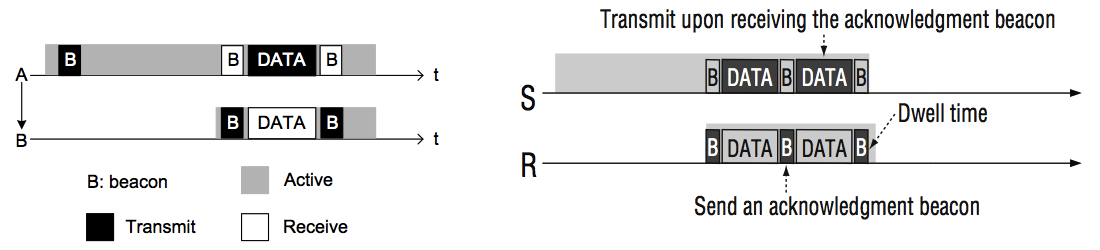
\includegraphics[width=14cm]{images/ch3-lpp.png}
\flcaption{Principe de transmission de données entre un noeud émetteur
(\textbf{A} ou \textbf{S}) et un noeud récepteur (\textbf{B} ou
\textbf{R}), selon la méthode RI-LPP (\lang{Receiver-Initiated
Low Power Probing}).
(Source~: \cite{coursEnsem} et \cite{Evolution-MAC-WSN-Survey-2013})}
\label{FigPrincipeLPP}
\end{figure}

Par rapport aux protocoles LPL, ce principe de fonctionnement permet
de réduire l'occupation moyenne du médium radio par un couple de
noeuds pour arriver à un point de rendez-vous.
En outre, les phénomènes de collisions cachées entre noeuds sont
également moins fréquents.

L'un des principaux problèmes du principe LPP survient lorsque
plusieurs noeuds ont simultanément besoin d'envoyer des données
au même destinataire~: à la réception du \lang{``beacon''} émis par ce
dernier, les différents noeuds émetteurs vont tous émettre leurs
trames de données, ce qui provoquera inévitablement une collision.
La probabilité que plusieurs noeuds cherchent à envoyer des données
au même noeud au même moment est d'autant plus forte que le trafic
du réseau concerné devient important.

Pour pallier ce problème, RI-MAC ajoute au principe LPP de base
une notion de \lang{``backoff''} intégrée aux \lang{``beacons''}~:
ces derniers incluent en effet une durée maximale de <<~silence~>>
parmi laquelle les noeuds émetteurs devront choisir aléatoirement
un délai à respecter entre la réception de ce \lang{``beacon''} et
l'envoi de leurs données. Au début, cette fenêtre de \lang{``backoff''}
est nulle~; à chaque collision détectée, cette fenêtre va voir
sa valeur augmenter rapidement pour minimiser les risques de nouvelle
collision. Cette procédure est appelée BEB (\lang{Binary Exponential
Backoff}), et est illustrée dans la figure \vref{FigBEBRIMAC}.

\begin{figure}[!hbt]
\centering
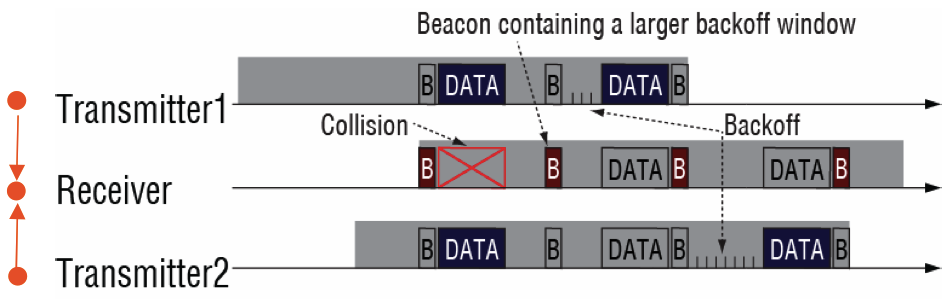
\includegraphics[width=12.5cm]{images/ch3-ri-mac-backoff.png}
\flcaption{Illustration de la méthode BEB (\lang{Binary Exponential
Backoff}) employée par RI-MAC pour résoudre les problèmes de
collisions dûs à l'envoi simultané de trames par plusieurs
émetteurs.
(Source~: \cite{coursEnsem} d'après \cite{RIMAC})}
\label{FigBEBRIMAC}
\end{figure}

On peut noter que cette procédure de BEB est similaire au mécanisme de
\lang{``backoff''} utilisé par la méthode CSMA/CA, également dans le but
de résoudre les cas de collisions.

\medskip

Grâce à ces mécanismes de fonctionnement, RI-MAC peut obtenir de meilleurs
résultats que X-MAC quand le trafic réseau est élevé, tout en ayant
un cycle de fonctionnement similairement bas (donc aussi économe en
énergie) quand le trafic est faible.

De façon générale, on constate que les protocoles basés sur le principe
RI (\lang{Receiver Initiated}) sont nettement plus performants quand le
trafic réseau est intense et/ou soumis à des interférences, là où les
protocoles laissant l'initiative de la transmission aux émetteurs vont
<<~étouffer~>> le réseau avec des collisions de trames de données.
Cela est nettement visible dans le schéma présenté dans la figure
\vref{FigRIvsSI}. On y voit que les protocoles
\lang{``Receiver-Initiated''} (LPP) ont toujours un net avantage,
d'autant plus flagrant que le débit augmente.

\begin{figure}[!hbt]
\centering
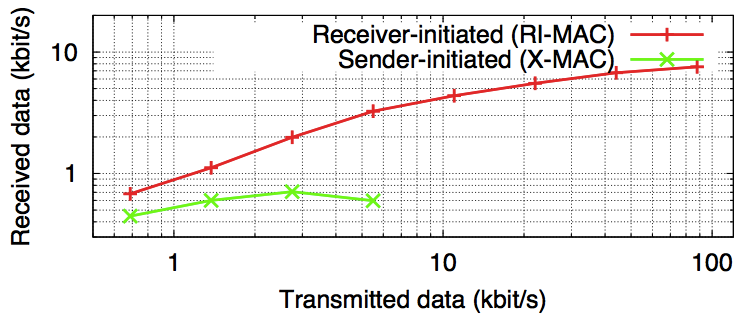
\includegraphics[width=12.5cm]{images/ch3-ri-vs-si.png}
\flcaption{Comparaison entre protocoles \lang{``Receiver-Initiated''} (LPP)
et \lang{``Sender-Initiated''} (LPL) face à la montée en charge
du trafic réseau.
(Source~: \cite{coursEnsem} d'après \cite{Strawman})}
\label{FigRIvsSI}
\end{figure}

Néanmoins, l'utilisation du médium radio par la méthode LPL (même améliorée
par RI-MAC) est toujours loin d'être optimale, le recours aux \lang{backoffs}
aléatoires pour éviter les collisions provoquant des <<~temps morts~>> où
le réseau doit rester inutilement silencieux.


\subsection{Protocoles MAC à ordonnancement temporel}
\label{SubsecProtoMACTDMA}

Tous les protocoles que nous avons vus jusqu'ici sont basés sur la
\emph{contention}~: les trames de données sont émises sur un médium radio
non réservé, ce qui implique un risque de collision et donc de perte de
données (ce qui nécessite en général un mécanisme de vérification et de
réémission des données si besoin est).

À l'inverse, les protocoles MAC dit \emph{ordonnancés} définissent
strictement l'occupation du médium radio, en allouant une partie
précise de la bande passante à chaque transmission potentielle, éliminant
ainsi les collisions.

La méthode employée pour parvenir à cette fin est basée sur le multiplexage
temporel~: chaque transmission se voit allouer le canal radio durant un
intervalle de temps bien défini. Cette méthode de fonctionnement est nommée
\nom{TDMA} (\lang{Time Division Multiple Access}). Son fonctionnement est
très similaire à la CFP observée plus haut dans le protocole MAC du standard
IEEE 802.15.4 en <<~mode \lang{``beacon''}~>>.

\begin{itemize}

\item Les protocoles basés sur la méthode TDMA sont considérés comme les
plus efficaces pour le traitement de trafics réseaux intenses, car ce sont
ceux qui permettent d'exploiter le plus efficacement le médium radio, et
donc d'approcher le plus de son débit maximal théorique.

\item Par contre, la nécessité de réserver au préalable les différents
intervalles de temps, quelle que soit l'intensité du trafic réseau, entraîne
un surcoût d'organisation (\lang{``overhead''}), ce qui rend les protocoles
basés sur la contention plus efficaces pour les faibles trafics. Les réseaux
de capteurs sans-fil actuels n'ayant le plus souvent à gérer qu'un faible
trafic (avec éventuellement quelques pointes), cela explique que les
protocoles basés sur la contention restent actuellement les plus utilisés.

\end{itemize}

Tout ceci est résumé de façon claire et synthétique dans le schéma présenté
dans la figure \vref{FigTDMAvsCSMA}. On y voit que la contention (CSMA)
gère mieux les faibles trafics, tandis que l'ordonnancement (TDMA) est plus
efficace pendant les débits intenses (ou les pointes de trafic réseau).

\begin{figure}[!hbt]
\centering
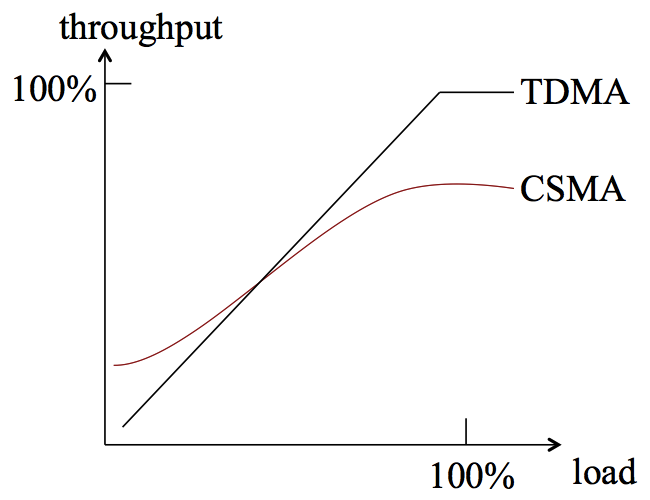
\includegraphics[width=10cm]{images/ch3-tdma-vs-csma.png}
\flcaption{Comparaison de l'efficacité entre méthodes basée sur la
contention (CSMA) et sur l'ordonnancement (TDMA) en fonction du débit
réseau.
(Source~: \cite{coursEnsem})}
\label{FigTDMAvsCSMA}
\end{figure}

En outre, toujours à cause de la nécessité d'organisation préalable
du multiplexage temporel du médium radio, les protocoles basés sur
l'ordonnancement sont en général du type synchrone, bien mieux adapté.

\subsubsection{LMAC}
\label{ParLMAC}

Le protocole LMAC \cite{LMAC} est un exemple typique de protocole basé
sur la méthode TDMA. Chaque cycle de fonctionnement (ou <<~trame~>>)
est divisé en \lang{``slots''}, représentant une unité minimale de temps
qui sera réservée à un noeud donné. Chaque noeud du réseau se verra
attribuer un \lang{slot} donné au sein de chaque trame réseau.

Durant son \lang{slot} de temps, un noeud doit d'abord émettre un
message de contrôle~--- indiquant s'il a des données à transmettre,
et si oui quel est leur destinataire~--- suivi s'il y a lieu du trame
de données à émettre.

Tous les noeuds du réseau doivent ainsi avoir leur émetteur~/ récepteur
radio activé pour écouter le message de contrôle émis au début de chaque
\lang{slot}. Les noeuds n'étant pas destinataires d'un message durant ce
\lang{slot} peuvent ensuite désactiver leur radio (donc tous les
noeuds si aucune donnée n'est à émettre durant ce \lang{slot}).

À noter que l'allocation des slots ne se fait pas de façon centralisée~:
au démarrage du réseau, chaque noeud doit choisir un \lang{slot} parmi
ceux disponibles, et le réserver pour les trames suivantes en y émettant
un message de contrôle.

\subsubsection{AI-LMAC}
\label{ParAILMAC}

Le protocole AI-LMAC \cite{AILMAC} est une extension de LMAC permettant
à un noeud de réserver plusieurs \lang{slots} au sein de chaque trame.
Le choix du nombre de \lang{slots} à allouer à chaque noeud n'est pas
faite de façon distribuée (comme pour la réservation), mais par le
coordinateur du réseau en fonction du trafic sortant prévu pour
chaque noeud.


\subsection{Protocoles MAC multicanaux}
\label{SubsecProtoMACFDMA}

Une dernière catégorie de protocoles MAC repose sur la capacité de la
couche physique 802.15.4 d'exploiter plusieurs canaux (c'est-à-dire
plusieurs fréquences) radio différents. Ainsi, tout comme il est possible
de multiplexer les différentes transmissions dans le temps, cette
fonctionnalité de la couche physique permet d'effectuer un multiplexage sur
les fréquences radio~: en assignant des canaux différents aux différents
noeuds d'un réseau, il devient possible de gérer des transmissions de
données parallèles.

Par analogie avec l'acronyme TDMA vu section \vref{SubsecProtoMACTDMA},
cette méthode de multiplexage sur les fréquences radio est appelée
\nom{FDMA} (\lang{Frequency Division Multiple Access}).

Les deux principales difficultés pour la conception de tels protocoles sont~:
\begin{itemize}
\item la distribution des différents canaux aux différents noeuds
d'un réseau~; et
\item la gestion efficace de la communication entre ces différents canaux.
\end{itemize}
Le deuxième point est rendu particulièrement difficile, car les émetteurs~/
récepteurs radio conçus pour le standard 802.15.4 ne sont pas capables
d'écouter simultanément plusieurs fréquences.
En outre, le standard 802.15.4 limitant la taille des trames physiques
à 127 octets, un mécanisme d'attribution des canaux aux différents noeuds
peut rapidement entraîner un surcroît de charge (\lang{``overhead''})
intolérable pour un réseau de ce type.

Différents protocoles ont été proposés pour contourner ces difficultés,
la tendance actuelle étant de combiner multiplexage temporel et multiplexage
fréquentiel~: on parle ainsi de protocoles TDMA/FDMA. Parmi ces protocoles,
on peut citer MC-LMAC employant cette méthode pour gérer les envois de
reales de données, ainsi que Y-MAC et MuChMAC employant une méthode
de <<~saut de fréquence~>> (\lang{``channel hopping''}) pour permettre
aux différents noeuds de recevoir des trames de données de plusieurs
canaux différents.

Ces protocoles multicanaux n'ayant pas été traités lors des présents
travaux de thèse, nous ne les étudierons pas plus en détail ici~;
l'étude de référence (\lang{``survey''}) de
\cite{Evolution-MAC-WSN-Survey-2013} consacrant toute sa section V
à l'étude de ces protocoles, nous invitons le lecteur souhaitant plus
de détails sur ce sujet à s'y reporter.

Il est par contre plus important de noter que l'amendement \nom{802.15.4e}
du standard, adopté en 2012, consacré à l'amélioration de la couche MAC
officielle du standard IEEE \cite{IEEE802154e-2012}, inclut un mécanisme
nommé \lang{``Time Slotted Channel Hopping''} ou \nom{TSCH}. Plus qu'une
simple amélioration, il s'agit tout simplement d'une nouvelle couche MAC,
totalement compatible avec la couche physique définie dans les précédentes
versions du standard 802.15.4, employant multiplexage temporel \emph{et}
multiplexage fréquentiel pour parvenir à une consommation d'énergie
minimale et une fiabilité de transmission maximale.

Une version dédiée de la pile IPv6 destinée à fonctionner par-dessus cette
nouvelle couche MAC et son mécanisme TSCH est déjà en cours de conception
par l'IETF, sous le nom de projet <<~6TiSCH~>> \cite{6TiSCH}. Cette nouvelle
pile protocolaire est notamment destinée à être supportée par la pile
réseau avancée \nom{OpenWSN} \cite{OpenWSN}, dont nous reparlerons
dans plus loin dans le présent chapitre (section \vref{SubsecRIOTOS}
sur RIOT OS et section \vref{SubsecFreeRTOS} sur FreeRTOS).

Notons toutefois que cette couche MAC est largement plus complexe que celles
définies dans les versions précédentes du standard (et que nous avons
étudiées section \vref{Subsec802154MAC}). Sa mise en oeuvre pourrait
par conséquent poser des difficultés sur les appareils à fonctionnalités
réduites (RFD) susceptibles de faire partie d'un réseau de capteurs sans-fil.
La description de cette nouvelle couche MAC complexe sort du cadre du
présent manuscrit de thèse et ne sera donc pas entreprise ici.

Malgré ces limitations, le standard IEEE 802.15.4e proposant désormais une
couche MAC officielle reposant sur le paradigme TDMA/FDMA, ce mode de
fonctionnement sera sans doute appelé à devenir incontournable dans
l'implantation des réseaux de capteurs sans-fil du futur.

\bigskip

Après l'étude des principales catégories <<~standard~>> de protocoles MAC,
et d'exemples représentatifs de ces dernières, nous allons maintenant nous
focaliser sur les protocoles avancés ayant fait l'objet des travaux de
la présente thèse.


\subsection{Protocoles hybrides avancés}
\label{SubsecProtoMACavances}

Des recherches sur la conception de protocoles MAC ont également été menées
au sein du centre INRIA Nancy Grand-Est et du LORIA. Ces recherches ont
notamment abouti à la conception de plusieurs protocoles évolués, qui ont
été à la base des travaux menés dans la présente thèse. Nous allons dans
la présente section examiner successivement ces différents protocoles
sur lesquels nous nous sommes focalisés.

Nous aborderons également brièvement~--- pour compléter notre tour d'horizon
des protocoles avancés~--- dans une autre sous-section les travaux d'autres
équipes de recherche sur d'autres protocoles MAC avancés.

Nous évoquerons aussi la couche MAC contenue dans une pile protocolaire
intégrée et complète, issue d'un effort de développement suivant une approche
dite multi-couches (en anglais \lang{``cross-layer''} dans une dernière
sous-section. De telles approches sortent toutefois du cadre de cette thèse,
laquelle se focalise sur les seules couches basses, et ne font par conséquent
l'objet d'aucun travail dans cette thèse.

\subsubsection{CoSenS et S-CoSenS}
\label{ParSCoSenS}

Ce protocole, conçu par B. Nefzi et Y.-Q. Song \cite{CosensConf}
\cite{CosensJournal}, fait partie de la classe des protocoles basés sur
la contention. Il est décrit dans le chapitre 3 de la thèse
de B. Nefzi \cite{TheseBNefzi}.

Le but de ce protocole est d'améliorer les performances de la couche
MAC notamment concernant la qualité de service, tout en limitant les coûts
liés à l'implantation de cette couche, ce qui exclut le recours à la
méthode TDMA (celle-ci nécessitant une configuration minutieuse
du réseau, une précision très fine de la synchronisation entre noeuds,
et une adaptation difficile aux changements de trafic sur le réseau).

Le protocole CoSenS reprend donc la méthode CSMA/CA, en contrôlant
les instants où se déroulent les transmissions et où le médium radio
est utilisé. Le principe de base est de séparer temporellement la période
où un noeud reçoit des trames de données (période de réception) de celle
où ce même noeud émet les trames ainsi reçues (période de retransmission).
Ceci est schématisé dans la figure \vref{FigCoSenSBase}. On voit que
chaque cycle CoSenS est partagé entre une période de réception (ou période
d'écoute~: WP) durant laquelle le noeud collecte les trames reçues,
suivi d'une période de transmission (TP) durant laquelle tous les trames
collectées dans la file d'envoi sont transmises vers la destination
adéquate. (Les trames~/ paquets collectés pouvant éventuellement être
traités par les couches supérieures de la pile de façon arbitraire
entre réception et émission).

\begin{figure}[!hbt]
\centering
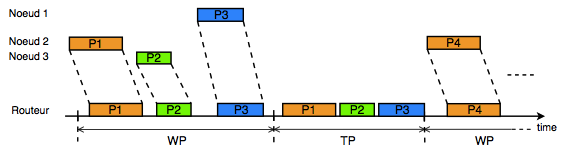
\includegraphics[width=12.5cm]{images/ch3-cosens-base.png}
\flcaption{Principe de base du protocole CoSenS.
(Source~: \cite{TheseBNefzi})}
\label{FigCoSenSBase}
\end{figure}

Il a été démontré que ce protocole apporte une amélioration sensible
des performances et de la qualité de service~--- notamment au niveau
du taux de succès de transmission des trames, du débit réseau maximal
supporté, ainsi que du délai de transmission de bout-en-bout des données~---
par rapport au protocole MAC de base du standard 802.15.4.

\newpage

Son principal défaut est par contre de nécessiter que tous les noeuds
gardent leur émetteur~/ récepteur radio allumé en permanence, ce qui
représente un sérieux désavantage concernant l'économie d'énergie.

C'est pourquoi ce protocole a été amélioré pour inclure une période
de sommeil dans le cycle de fonctionnement des noeuds. Le protocole
résultant est nommé \nom{S-CoSenS}, et c'est celui sur lequel nous
nous sommes principalement basés lors de nos travaux de thèse. Il s'agit
donc à la fois d'un protocole MAC et d'un protocole RDC (\lang{Radio
Duty Cycle}~: gérant le cycle d'allumage et d'extinction de l'émetteur~/
récepteur radio), qui plus est adapté aux phases de routage. Il est décrit
dans le chapitre 5 de la thèse de B. Nefzi \cite{TheseBNefzi}.

Tout comme CoSenS, il est basé sur la méthode CSMA/CA, et est ainsi
comparable à la couche MAC 802.15.4 en <<~mode sans \lang{``beacon''}~>>.
L'idée de base reste de retarder la retransmission des trames reçues,
en divisant chaque cycle de fonctionnement d'un noeud coordinateur
en trois périodes~:
\begin{itemize}
\item une période de sommeil (SP~: \lang{Sleeping Period}) où l'émetteur~/
récepteur radio est désactivé pour économiser l'énergie du noeud~;
\item une période d'écoute ou période d'attente (WP~: \lang{Waiting Period})
durant laquelle le médium radio est écouté pour collecter les trames de
données 802.15.4 arrivantes~;
\item et une période de transmission (TP~: \lang{Transmission Period})
durant laquelle les trames reçues et mis en attente durant la période
d'écoute sont réémises, si possible en lot (\lang{``burst''}).
\end{itemize}

Le principal avantage de S-CoSenS est son capacité à s'adapter dynamiquement
à l'intensité du trafic radio en temps réel, en calculant pour chaque cycle
radio (commun à tout un PAN fonctionnant sous S-CoSenS) la durée des
périodes de sommeil (SP) et d'écoute (WP), en fonction du nombre de
trames retransmises durant les cycles précédents.

Notons que l'ensemble constitué de la période de sommeil (SP) et de la
période de réception (WP) d'un même cycle est appelé \nom{subframe}~;
il s'agit de la partie du cycle de S-CoSenS dont la durée est calculée
et connue \lang{a priori}. À l'inverse, la durée de la période d'envoi (TP)
ne peut être déterminée qu'à son tout début, car cette durée dépend
directement de la quantité de trames de données reçues avec succès
durant la période d'écoute (WP) précédente.

En outre, le calcul de la durée de la période d'envoi WP se fait via un
algorithme de <<~moyenne glissante~>>, où la durée de WP pour chaque cycle
est calculée ainsi~:
\begin{eqnarray*}
&&
\overline{\mathrm{WP}_{n}} = \alpha \cdot \overline{\mathrm{WP}_{n-1}}
                + (1 - \alpha) \cdot \mathrm{WP}_{n-1}
\\ &&
\mathrm{WP}_{n} = \max ( \mathrm{WP}_{min},
                  \min ( \overline{\mathrm{WP}_{n}}, \mathrm{WP}_{max} ) )
\end{eqnarray*}
où $\overline{\mathrm{WP}_{n}}$ et $\overline{\mathrm{WP}_{n-1}}$
sont respectivement la durée moyenne de WP au $n^{\mathrm{eme}}$ et
$(n-1)^{\mathrm{eme}}$ cycle, tandis que $\mathrm{WP}_{n}$ et
$\mathrm{WP}_{n-1}$ sont les durées réelles de WP respectivement
au $n^{\mathrm{eme}}$ et $(n-1)^{\mathrm{eme}}$ cycles;
$\alpha$ est un paramètre dont la valeur est arbitrairement choisie
entre 0 et 1, représentant le poids relatif de l'historique dans le
calcul des durées~; $\mathrm{WP}_{min}$ et $\mathrm{WP}_{max}$ étant
les limites minimales et maximales imposées à la durée de WP par
le programmeur.

La synchronisation locale entre un routeur S-CoSenS et ses noeuds-feuilles,
au sein d'un même PAN, se fait grâce à une trame \lang{``beacon''}
émis par le routeur au début de chaque cycle. Ce \lang{``beacon''} inclut
les durées (en microsecondes) choisies pour la période de sommeil (SP) et
la période de réception (WP) au cours du cycle dont le \lang{``beacon''}
marque le début.

La représentation schématique d'un cycle complet S-CoSenS,
du point de vue d'un routeur gérant un PAN, est décrite dans la figure
\vref{FigCycleSCoSenS}. On distingue la période de sommeil (SP),
la période d'écoute~/ réception (WP) et la période de retransmission (TP).
L'ensemble des deux premières périodes constitue la \lang{subframe},
dont la durée est calculée à l'avance, en fonction du trafic
réseau observé jusqu'alors.

La figure \vref{FigCycleSCoSenS} montre clairement l'adaptation
du cycle S-CoSenS à un trafic réseau moyen (a), intense (b) et faible (c).

\begin{figure}[!hbt]
\centering
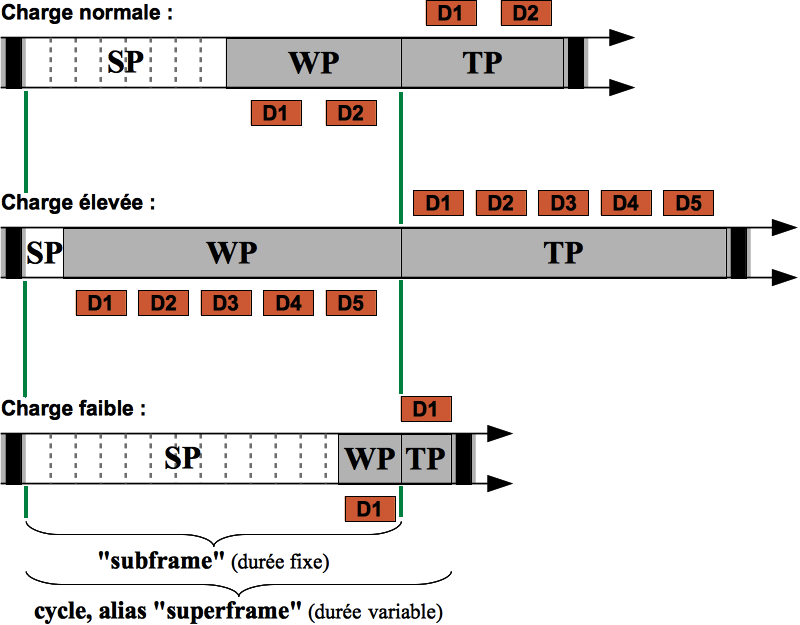
\includegraphics[width=10cm]{images/ch3-s-cosens-cycle.png}
\flcaption{Principe d'un cycle de fonctionnement d'un noeud coordinateur
S-CoSenS. (Source~: \cite{TheseBNefzi})}
\label{FigCycleSCoSenS}
\end{figure}

Cette synchronisation locale au sein d'un PAN S-CoSenS, faite grâce
à l'envoi cyclique d'un \lang{``beacon''}, repose donc sur le paradigme
LPP (\lang{Low Power Probing}, principe détaillé plus haut). D'un
autre côté, la synchronisation et la communication entre routeurs
S-CoSenS appartenant à des PANs différents se fait grâce à de courtes
périodes d'éveil et d'écoute se déroulant durant la période de sommeil
(SP), et repose donc sur le paradigme LPL (\lang{Low Power Listening},
comme pour X-MAC par exemple), pour des raisons de simplicité.

À noter que le cycle S-CoSenS complet (SP + WP + TP) ne concerne que
les noeuds jouant le rôle de routeur et de coordinateur de PAN.

En effet, une propriété intéressante de S-CoSenS est que les noeuds
terminaux ou noeuds-feuilles (c'est-à-dire ceux n'ayant pas un rôle de
routeur ou de coordinateur de réseau) peuvent garder leur émetteur~/
récepteur radio constamment éteint, tant qu'ils n'ont pas de trame
à envoyer. Quand un de ces noeuds-feuilles doit envoyer une trame de
données, il démarre sa radio, écoute et attend le premier \lang{``beacon''}
émis par un routeur, puis émet sa trame en utilisant la méthode
CSMA/CA au début de la période de réception (WP) annoncée dans le
\lang{``beacon''} qu'il a reçu. Ce noeud-feuille peut éteindre sa radio
pendant le délai courant entre le \lang{``beacon''} et la WP attendue
(c'est-à-dire durant le délai correspondant à la période de sommeil
SP du routeur ayant émis le \lang{``beacon''}), émet sa trame durant
la WP voulue, puis peut retourner à l'état de sommeil une fois sa
trame transmise avec succès.

Toute cette procédure de transmission est résumée dans la figure
\vref{FigSCoSenSTransmission}. Dans cette figure, les parties grises
représentent les périodes où un noeud fait fonctionner sa radio,
les blocs oranges correspondent aux transmissions de trames, tandis que
les parties blanches sont celles où le noeud met sa radio en sommeil pour
économiser son énergie. Le noeud simple émetteur se réveille quand une
trame doit être émise, attend le \lang{``beacon''} issu du routeur,
se synchronise alors pour émettre la trame durant la période de réception
(WP) du routeur, puis retourne en mode sommeil. Le routeur peut ensuite
réemettre la trame vers la destination adéquate durant sa période
de transmission (TP).

\begin{figure}[!hbt]
\centering
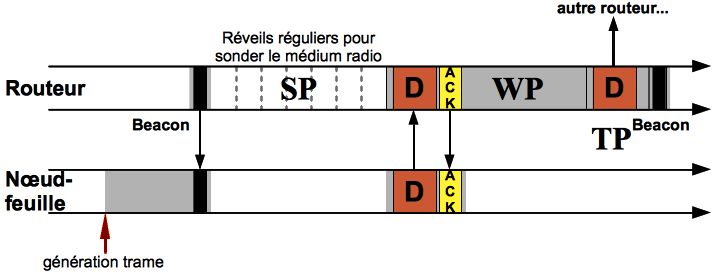
\includegraphics[width=9.5cm]{images/ch3-s-cosens-transmission.png}
\flcaption{Transmission d'une trame avec le protocole S-CoSenS.}
\label{FigSCoSenSTransmission}
\end{figure}

\bigskip

Si ce protocole représente une amélioration certaine par rapport
au protocole MAC de base du standard 802.15.4 et aux protocoles
LPL et LPP classiques~--- comme nous le verrons dans le chapitre
\ref{ChProtocolesMAC} de la présente thèse~---, il continue néanmoins
de souffrir des limitations intrinsèques liées au principe de contention
sur lequel il est basé~: lors de trafics réseaux intenses, la qualité
de service (taux de trames transmises avec succès, délais de
transmission) chute irrémédiablement. Ces problèmes sont mieux
pris en charge par les protocoles basés sur l'ordonnancement
(TDMA) mais ceux-ci posent d'autres problèmes (complexité,
lourdeur d'organisation). Des recherches ont donc été menées
pour contourner ces problèmes, et ont abouti à la mise au
point de nouveaux protocoles plus performants, dont celui
que nous allons maintenant détailler dans la section
\ref{PariQueueMAC} suivante.

\subsubsection{iQueue-MAC}
\label{PariQueueMAC}

Ce protocole, de conception récente et ambitieuse \cite{iQueueMAC}, est un
protocole ordonnancé hybride, utilisant la contention (méthode CSMA/CA)
et l'ordonnancement temporel (TDMA) en fonction du trafic réseau courant.

Nous avons vu en effet plus haut qu'il a été démontré que la méthode CSMA
est plus efficace pour le traitement des faibles trafics, tandis que TDMA
est nettement plus appropriée pour supporter les trafics intenses.

Si le protocole MAC standard 802.15.4 en <<~mode \lang{``beacon''}~>> fait
déjà appel à une approche hybride (avec les notions de CAP et CFP), il est
limité par la configuration totalement statique de ses paramètres de
fonctionnement.

À l'inverse, iQueue-MAC est conçu pour s'adapter dynamiquement et en
temps réel au trafic du réseau, de façon à adopter à chaque instant la
meilleure configuration pour optimiser qualité de service et consommation
d'énergie (via la maîtrise du \lang{duty cycle} et de ses différentes
périodes, dont les durées sont dynamiques).

La figure \vref{FigiQueueMACCharge} montre comment iQueue-MAC gère la
montée en charge du trafic réseau de façon totalement différente d'autres
protocoles plus classiques basés sur la seule contention (comme par exemple
S-CoSenS).

\begin{figure}[!hbt]
\centering
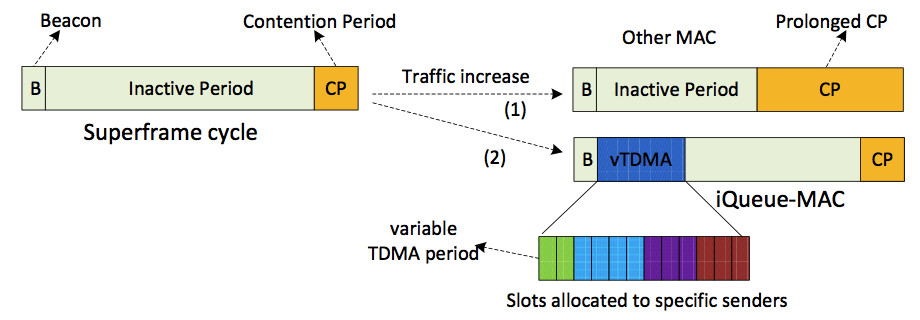
\includegraphics[width=12.5cm]{images/ch3-iqueue-mac-charge.png}
\flcaption{Comparaison de la gestion de la montée en charge du trafic
réseau entre \textbf{(1)}~un protocole uniquement basé sur la contention,
et \textbf{(2)}~iQueue-MAC, qui a recours à une période basée sur TDMA
de durée variable, adaptée à la charge réseau.
(Source~: \cite{coursEnsem})}
\label{FigiQueueMACCharge}
\end{figure}

Les idées principales qui sous-tendent la conception d'iQueue-MAC sont
les suivantes~:
\begin{itemize}
\item L'utilisation de la contention (CSMA/CA) quand le trafic est faible,
et de l'ordonnancement temporel (TDMA) quand le trafic devient intense.
\item La séparation des noeuds sans-fil en deux catégories~: les noeuds
simples (terminaux ou noeuds-feuilles) et les routeurs.
\item Les noeuds simples (tout comme avec la famille CoSenS) ne s'éveillent
que quand ils ont des données à envoyer, et passent donc la majeure partie
de leur temps en sommeil pour économiser leur énergie.
\item Les routeurs sont les noeuds exécutant véritablement la totalité
du mécanisme d'iQueue-MAC.
\item Le protocole base son comportement et sa configuration sur la
connaissance de la quantité de trames à envoyer (c'est-à-dire la
longueur de la file d'envoi de trames) pour chaque noeud du réseau.
\end{itemize}

En effet, chaque noeud simple, lorsqu'il envoie une trame, insère le
niveau d'occupation de sa file d'envoi (juste après l'entête de la trame).
Le routeur est donc à chaque cycle capable d'évaluer la charge que
devra soutenir le réseau lors du cycle suivant. La structure d'une
trame iQueue-MAC est représentée figure \vref{FigiQueueMACTrame}.
On notera l'ajout du taux d'occupation de la file d'envoi du noeud émetteur
entre l'entête MAC et la charge utile (\lang{``payload''}) de la trame
proprement dite.

\begin{figure}[!bpt]
\centering
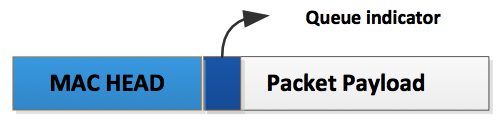
\includegraphics[width=7.5cm]{images/ch3-iqueue-mac-paquet.png}
\flcaption{Structure d'une trame iQueue-MAC.
(Source~: \cite{coursEnsem})}
\label{FigiQueueMACTrame}
\end{figure}

Chaque cycle iQueue-MAC (également appelé \nom{superframe}, est
représenté figure \vref{FigiQueueMACCycle}. La \lang{subframe} est
la partie du cycle dont la durée est calculée (donc connue) à l'avance~;
elle comporte la période TDMA, dont la durée varie en fonction de
l'intensité du trafic réseau, et dont les \lang{slots} temporels
sont alloués aux différents noeuds en fonction de la quantité
de trames qu'ils ont à émettre (ces quantités ayant été transmises
durant la période de contention du cycle précédent).

Un cycle iQueue-MAC se décompose donc en les phases suivantes~:
\begin{description}
\item[B~: \lang{``beacon''}.]
Celui-ci permet la synchronisation des différents noeuds du PAN~:
il indique la durée et l'affectation des différents \lang{slots} de la
période TDMA, ainsi que la durée de la période de sommeil. L'ensemble
regroupant les slots de temps TDMA et la période de sommeil est appelé
\emph{subframe}~: c'est la partie du cycle iQueue-MAC dont la durée est
calculée et allouée à l'avance. La structure d'un \lang{``beacon''}
iQueue-MAC est détaillée figure \vref{FigiQueueMACBeacon}.
Toutes les données nécessaires pour calculer la durée de la
\lang{subframe}, de la section TDMA variable, et l'allocation
des différents \lang{slots} de temps TDMA aux différents noeuds
demandeurs sont présentes.

\begin{figure}[!bpt]
\centering
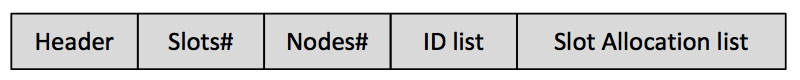
\includegraphics[width=9cm]{images/ch3-iqueue-mac-beacon.png}
\flcaption{Structure d'un \lang{``beacon''} iQueue-MAC.
(Source~: \cite{coursEnsem})}
\label{FigiQueueMACBeacon}
\end{figure}

\item[SF~: \lang{SubFrame}]
Cette période contient les slots de temps TDMA dont l'allocation aux
différents noeuds a été annoncée dans le \lang{``beacon''}~; ces slots TDMA
sont suivis de la période de sommeil où la radio du routeur est éteinte
pour économiser l'énergie. Notons que comme dans d'autres protocoles tels
que X-MAC ou S-CoSenS, de courts moments d'activation de la radio ont lieu
durant la période de sommeil, afin de pouvoir détecter et recevoir des
messages en provenance de routeurs d'autres PANs.
\item[CP~: \lang{Contention Period}]
Période de réception basée sur le principe de la contention (CSMA/CA) où
chaque noeud du PAN est autorisé à transmettre une et une seul trame~---
s'il a plus d'une trame de données à transmettre, l'indicateur de
remplissage de sa file d'envoi situé au début de la charge utile
(\lang{``payload''}) de la trame lui fera allouer le nombre de \lang{slots}
nécessaires durant la \lang{subframe} du cycle suivant. La durée de la CP
n'est pas prédéterminée~: le routeur écoute jusqu'à la survenue d'un
\lang{timeout} d'inactivité radio, ce qui est censé donner assez de temps
à chaque noeud ayant des données à émettre (principe similaire à celui
vu plus haut pour T-MAC).
\item[TP~: \lang{Transmission Period}]
La retransmission des trames par le routeur~--- vers le routeur suivant
ou le concentrateur final~/ station de base du réseau sans fil
(\lang{``sink''})~--- se fait par lots (en mode \lang{``burst''}),
comme par exemple pour les protocoles T-MAC ou RI-MAC vus plus haut~:
une fois la première trame envoyée avec succès, les trames suivantes
sont envoyées avec un minimum \lang{d'overhead}.
\end{description}

\begin{figure}[!bpt]
\centering
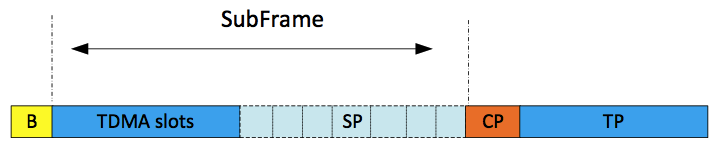
\includegraphics[width=12cm]{images/ch3-iqueue-mac-cycle.png}
\flcaption{Structure d'un cycle iQueue-MAC.
(Source~: \cite{coursEnsem})}
\label{FigiQueueMACCycle}
\end{figure}

\begin{figure}[!htb]
\centering
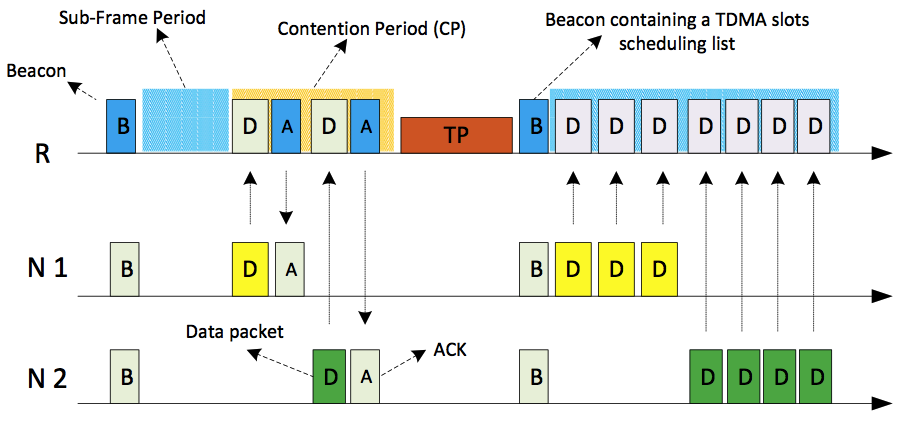
\includegraphics[width=12cm]{images/ch3-iqueue-mac-exemple-transmission.png}
\flcaption{Exemple de transmission de trames entre deux noeuds simples
et un routeur avec le protocole iQueue-MAC.
(Source~: \cite{coursEnsem})}
\label{FigiQueueMACExemple}
\end{figure}

\newpage

Donnons ici un exemple de déroulement d'une transmission d'un lot
de trames depuis deux noeuds simples vers un routeur iQueue-MAC,
tel que montré dans la figure \vref{FigiQueueMACExemple}~:
\begin{enumerate}
\item Soit un routeur R, et deux noeuds N1 et N2, ayant respectivement
4 et 5 trames de données à transmettre~; on suppose qu'aucune autre
transmission n'est en cours à ce moment-là dans ce PAN.
\item Pendant le premier cycle, N1 et N2 reçoivent le \lang{``beacon''}
de synchronisation. Aucun slot TDMA n'étant alloué, ils attendent tous
deux la période de contention CP, et émettent chacun leur première trame
de données~; la méthode CSMA/CA étant utilisée, ils reçoivent un
acquittement pour l'envoi de ces premières trames.
\item Le routeur termine son cycle par sa période de transmission TP,
et le premier cycle se termine.
\item Le routeur ayant reçu la taille des files d'envoi des deux
noeuds lors de la période de contention précédente, il alloue donc
le nombre de \lang{slots} TDMA nécessaire aux différents noeuds~:
3 pour N1, et 4 pour N2. Une fois les durées nécessaires calculées,
le second cycle commence, et un nouveau \lang{``beacon''} est envoyé.
\item Les noeuds N1 et N2 reçoivent ce \lang{``beacon''} et se synchronisent
pour l'envoi de leurs données durant la \lang{subframe}
\item Les trois premiers \lang{slots} TDMA étant alloués à N1, celui
envoie dès le début de la \lang{subframe} ses trames restantes. Sa file
d'envoi étant désormais vidée, il peut retourner en mode sommeil, jusqu'à
ce qu'il ait par la suite de nouvelles données à envoyer.
\item Les quatre \lang{slots} TDMA suivants étant alloués à N2, il
peut lui aussi envoyer à son tour les trames de données restant dans sa
file d'envoi, et à son tour passer en mode sommeil pour économiser son
énergie.
\item Toutes les données ayant besoin d'être transmises sont désormais
arrivées au routeur, qui peut terminer sa \lang{subframe} en période
de sommeil, puis retransmettre ces trames de façon adéquate durant
la période de transmission (TP) qui terminera ce second cycle (mais
n'est pas montrée sur la figure \vref{FigiQueueMACExemple}).
\end{enumerate}

\medskip

Les différentes expériences menées dans la publication \cite{iQueueMAC}
ont montré la nette supériorité d'iQueue-MAC en termes de qualité de
service~--- taux de trames transmises avec succès, délai total de
transmission~--- dans toutes les configurations, vis-à-vis de protocoles
tels que RI-MAC ou CoSenS (lequels avaient eux-mêmes déjà prouvé leur
supériorité sur les protocoles LPL classiques couramment utilisés).
Cette supériorité est notamment flagrante pour les charges réseaux intenses,
ou pour le traitement de pics soudains de trafic. Ce protocole semble donc
se poser en concurrent sérieux pour le nouveau protocole 802.15.4e~;
ce dernier ayant pour avantage sa capacité de traitement multicanal, tandis
que iQueue-MAC semble plus à même d'exploiter au mieux le débit maximal
théorique d'une unique fréquence radio, ce qui rend sa conception
et son implantation plus simple~--- avantage non négligeable lorsqu'il
s'agit d'implanter un protocole MAC sur un appareil à fonctionnalités
limitées (<<~RFD~>> standard IEEE 802.15.4).

\subsubsection{Autres évolutions de protocoles basés sur la contention}
\label{ParProtoTNoel}

Outre les protocoles avancés développés par notre équipe que nous avons
décrit ci-dessus dans les sections \vrefrange{ParSCoSenS}{PariQueueMAC},
d'autres équipes de recherche continuent également d'apporter de
nouvelles idées et techniques pour améliorer les performances et/ou
diminuer la consommation énergétique des protocoles MAC~/ RDC.

\smallskip

Nous citerons ici, à titre d'exemple, les travaux menés à l'Université
de Strasbourg pour améliorer les protocoles basés sur la technique LPL,
grâce notamment à un mécanisme nommé T-AAD (\lang{lightweight ``Traffic
Auto-ADaptations''} \cite{T-AAD}, conçu pour permettre aux protocoles LPL
de mieux gérer les pointes (\lang{``bursts''} de trafic réseau.

Le mécanisme \nom{T-AAD} consiste à adapter automatiquement les paramètres
des protocoles MAC dynamiquement en fonctions des variations du trafic
réseau. Le principal paramètre d'un protocole LPL étant la durée de la
période de sommeil (ici appelée $ST$) entre deux CCA consécutifs~---
c'est-à-dire en fait la durée du cycle de ces protocoles LPL~---,
T-AAD se propose d'alterner la durée de $ST$ entre deux extremums,
$ST_{min}$ et $ST_{max}$, selon la charge réseau. $ST_{max}$ est la durée
de cycle longue (par exemple, 500~ms), employée par défaut, lorsque la
charge réseau est à son niveau <<~de base~>>. $ST_{min}$ est la durée
de cycle courte (par exemple, 32~ms), utilisée temporairement afin
de prendre en charge efficacement les pointes de trafic réseau.

Afin de pouvoir estimer dynamiquement la charge réseau à venir, T-AAD
impose à chaque noeud d'ajouter, à chaque paquet émis, le nombre de paquets
lui restant à émettre dans sa file d'envoi. Un noeud récepteur employant
T-AAD utilise alors cette information pour calculer le temps durant lequel
il va passer sa durée de cycle à $ST_{min}$ pour gérer cette charge à venir~:
cette durée de fonctionnement <<~intensif~>> est nommée $T_{adapt}$.
Une fois la durée $T_{adapt}$ écoulée, le noeud revient à la durée de cycle
par défaut $ST_{max}$. (Notons que quand un noeud émetteur n'émet qu'une
charge réseau modérée, $T_{adapt}$ sera calculée à la valeur 0, et
le récepteur gardera alors un cycle standard de durée $ST_{max}$.)

Le but du mécanisme T-AAD est donc de rendre les protocoles LPL
<<~classiques~>> (comme X-MAC ou ContikiMAC) auto-adaptatifs à la charge
réseau, comme le sont naturellement CoSenS~/ S-CoSenS et iQueue-MAC.

Notons toutefois qu'il s'agit d'un mécanisme bien plus simple que pour
nos deux protocoles, la durée de cycle variant de façon discrète entre
deux valeurs, et non de façon continue et précise. L'avantage de T-AAD
est d'être ainsi d'une conception bien plus simple, au prix d'une
moindre précision dans l'adaptation de la durée des cycles MAC~;
toutefois, comme ce mécanisme doit s'adapter à des protocoles n'ayant
pas été au départ conçus pour être auto-adaptatifs, une telle simplicité
peut être considérée comme mieux adaptée à la cible choisie.

\medskip

Ce mécanisme T-AAD a été implémenté et testé pour améliorer des
protocoles LPL classiques comme X-MAC \cite{T-AAD} \cite{T-AAD-demo}
(se reporter respectivement à la section \vref{ParXMAC} pour les détails
sur le fonctionnement <<~standard~>> de ce protocole). Les changements
apportés par le mécanisme T-AAD dans le fonctionnement de X-MAC sont
illustrés dans la figure \vref{Fig-TAAD-XMAC}.

\begin{figure}[!htb]
\centering
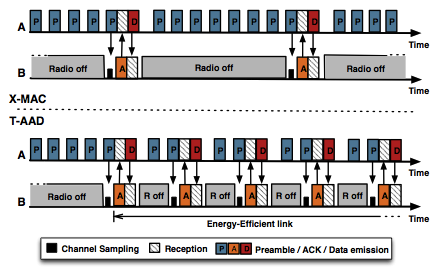
\includegraphics[width=11cm]{images/ch3-t-aad-x-mac.png}
\flcaption{Modification du fonctionnement du protocole X-MAC par le
mécanisme T-AAD. (Source~: \cite{T-AAD})}
\label{Fig-TAAD-XMAC}
\end{figure}

Il a été montré dans \cite{T-AAD} que ce mécanisme simple~--- donc
relativement facile à implémenter et peu coûteux en occupation mémoire
et en temps processeur~--- a permis d'améliorer significativement les 
performances (notamment en termes de délais de transmission) et
l'efficacité énergétique du protocole X-MAC ainsi modifié. Ces améliorations
ont été constatées par des tests faits sur du matériel réel, à savoir~:
les noeuds du \lang{testbed} IoT-LAB \cite{IotLAB}.

\bigskip

Plus récemment, cette même équipe a publié plusieurs versions améliorées
de ContikiMAC (cf. section \ref{ParContikiMAC} pour plus de détails sur
ce protocole MAC~/ RDC), destinées à être mieux adaptées aux noeuds mobiles,
nommées M-ContikiMAC et ME-ContikiMAC \cite{ME-ContikiMAC} (M signifiant ici
\lang{``Mobile''}, et ME \lang{``Mobile Enhanced''}.

Le protocole \nom{M-ContikiMAC} consiste à utiliser pour émettre ses trames
un mode de transmission \lang{``anycast''}, permettant à n'importe quel
noeud à portée de recevoir un paquet. Contrairement toutefois au mode
\lang{``broadcast''} que nous avons vu pour l'envoi de \lang{``beacons''},
en mode \lang{``anycast''} tout récepteur est tenu de renvoyer un paquet
d'acquittement, comme pour une transmission classique (également appelée
\lang{``unicast''}. Une fois un ou plusieurs récepteurs identifiés grâce
aux premiers envois de paquets en mode \lang{``anycast''}, les transmissions
suivantes de trames peuvent se faire de façon classique \lang{``unicast''}
suivant le mécanisme standard de ContikiMAC. Ce mode opératoire, bien
adapté aux noeuds mobiles ne pouvant compter sur des protocoles de routage
avancés pour découvrir leur entourage, peut être illustré grâce au schéma
montré en figure \vref{FigMContikiMAC} (où un noeud mobile communique
avec un noeud fixe parmi deux présents dans un WSN donné).

\begin{figure}[!htb]
\centering
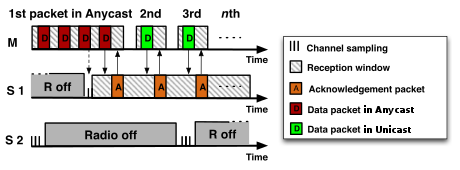
\includegraphics[width=10.75cm]{images/ch3-m-contikimac.png}
\flcaption{Fonctionnement du protocole avancé M-ContikiMAC, optimisé pour
les noeuds mobiles des WSN. (D'après \cite{ME-ContikiMAC})}
\label{FigMContikiMAC}
\end{figure}

\medskip

Sur la base de M-ContikiMAC, la même équipe a alors ensuite développé
\nom{ME-ContikiMAC}. Ce dernier protocole a notamment été conçu pour mieux
gérer les problèmes liés à la duplication des paquets et à l'optimisation
des délais de transmission, par rapport à M-ContikiMAC. Pour ce faire,
ME-ContikiMAC envoie désormais en \lang{``anycast''}, pour chercher
des récepteurs et établir des <<~connexions~>>, non plus des trames
de données (comme dans ContikiMAC), mais des trames de contrôle, dont
l'émission est maintenue même en cas de collision au niveau des paquets
d'acquittement, jusqu'à la réception d'un paquet d'acquittement correct.
L'envoi des trames de données se fait ensuite uniquement en
\lang{``unicast''}, jusqu'à la fin de la transmission ou la <<~perte
de connexion~>> (par exemple quand le noeud mobile n'est plus à portée).

Le fonctionnement de ME-ContikiMAC peut être illustré par la figure
\vref{FigMEContikiMAC}. On y voit notamment la façon dont ce protocole
gère les collisions et la déduplications de paquets, et ce avec
un noeud mobile communicant avec trois noeuds fixes.

\begin{figure}[!hbt]
\centering
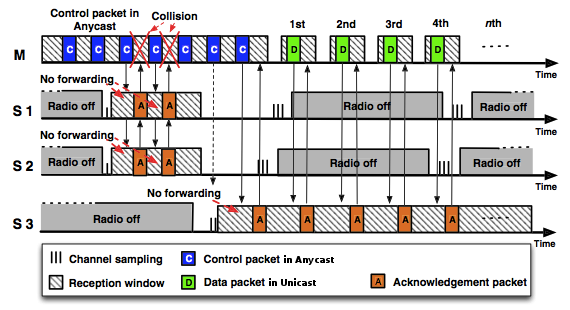
\includegraphics[width=12.75cm]{images/ch3-me-contikimac.png}
\flcaption{Fonctionnement du protocole avancé ME-ContikiMAC.
(D'après \cite{ME-ContikiMAC})}
\label{FigMEContikiMAC}
\end{figure}

Là encore, l'article \cite{ME-ContikiMAC} montre des améliorations
sensibles au point de vue de la qualité de service (déduplication de
paquets, occupation du médium radio, delais de transmissions réduits)
et de la consommation énergétique. ME-ContikiMAC a notamment montré,
dans ladite publication, que ces améliorations étaient sensibles vis-à-vis
de WSN ayant des noeuds statiques mais aussi et surtout des noeuds
mobiles. (Notons toutefois que cet article ne s'appuie, contrairement
aux publications sur T-AAD, que sur des simulations effectuées sous
Cooja).

\bigskip

On voit donc au final que de nombreuses équipes de recherches continuent
à explorer continuellement et activement de nombreuses pistes pour
améliorer les couches MAC~/ RDC des piles protocolaires des WSN,
que ce soit par la conception de protocoles entièrement nouveaux~---
tels CoSenS~/ S-CoSenS et iQueue-MAC~--- ou par l'invention de mécanismes
astucieux et efficaces pour améliorer les protocoles existants.

Les deux approches peuvent l'une comme l'autre permettre d'obtenir
des résultats significatifs en termes d'optimisation de la qualité
de service et de la consommation d'énergie. 

\subsubsection{Approches multi-couches~: l'exemple de la pile OCARI}
\label{ParOCARI}

Outre le seul développement de protocoles MAC~/ RDC~--- c'est-à-dire
de solutions relevant exclusivement de la couche 2 du modèle OSI~---,
plusieurs travaux consistant en le développement de piles protocolaires
complètes, pouvant aller jusqu'aux couches du plus haut niveau, ont été
menés. On peut noter que de tels travaux ont été menés plus souvent dans
un cadre industriel que dans celui de la recherche purement académique,
comme c'était majoritairement le cas des protocoles que nous avons vu
jusqu'ici dans cet état de l'art.

De telles approches, dites <<~multi-couches~>> ou \lang{``cross-layer''},
incluent donc une couche MAC qui, par définition, est intimement liée
au reste de la pile, et n'est \lang{a priori} pas conçue pour être
implantée de façon indépendante.

Un exemple d'une telle pile protocolaire complète, basé sur la couche
physique du standard IEEE 802.15.4 (sur la bande à 2,4~GHz uniquement)
est OCARI (Optimisation des Communications Ad-hoc pour les Réseaux
Industriels) \cite{OCARI}. Comme son nom l'indique, il s'agit ici d'un
effort de rechcerche appliquée~--- mené par une alliance regroupant
différents acteurs majeurs, industriels et académiques~--- destiné à
fournir une pile réseau à très haute fiabilité, afin d'offrir une
solution pour des applications critiques comme celles liées aux
centrales nucléaires ou aux navires militaires.

De cet effort est née une pile protocolaire complète, allant de la couche
MAC~/ RDC (niveau 2 OSI) aux API destinées à la programmation d'applications
(assimilable au niveau 7 OSI). Compte-tenu du sujet de notre thèse, nous
nous cantonnerons à l'étude de la couche MAC, nommée \nom{MaCARI}, bien que
celle-ci soit étroitement liée aux autres couches d'OCARI. Cette couche
est notamment prévue pour faciliter les opérations de routage, en
coopération étroite avec les couches supérieures d'OCARI.

L'organisation d'un cycle MaCARI se divise en trois périodes, et est
représentée sur la figure \vref{FigMaCARICycle}.

\begin{figure}[!htb]
\centering
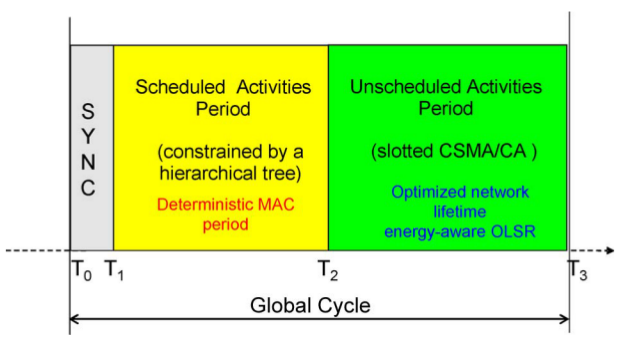
\includegraphics[width=10cm]{images/ch3-ocari-macari-cycle.png}
\flcaption{Structure d'un cycle du protocole MaCARI.
(Source~: \cite{OCARI} figure 3)}
\label{FigMaCARICycle}
\end{figure}

\smallskip

Ces trois périodes sont~:
\begin{enumerate}
\item une période de synchronisation des différents noeuds ($T_0$--$T_1$),
en gris sur la figure \vref{FigMaCARICycle}~;
\item une période de transmissions pré-déterminées ($T_1$--$T_2$), basée
sur une méthode TDMA optimisée, assurant une réservation de \lang{slots}
dépourvue de toute interférence pour toute transmission, en jaune sur
la  figure \vref{FigMaCARICycle}~;
\item une période de transmissions <<~spontanées~>> ($T_2$--$T_3$), basée
sur la contention (CSMA/CA slottée), en vert sur la figure
\vref{FigMaCARICycle}.
\end{enumerate}

Le protocole MaCARI est véritablement un protocole hybride, puisque l'on
peut le considérer à la fois comme un protocole synchrone, un protocole basé
sur le multiplexage temporel (TDMA), et un protocole basé sur la contention.
Il s'agit enfin d'un protocole MAC~/ RDC, l'émetteur~/ récepteur radio
pouvant être mis hors fonction pour économiser l'énergie durant la période
<<~déterministe~>> quand un noeud n'a pas à communiquer durant son
\lang{slot} assigné.

Si le protocole MaCARI est, comme on le voit, très performant et ingénieux,
son intégration étroite avec le reste de la pile OCARI~--- le rendant
délicat à porter et utiliser indépendamment de cette pile~--- et son
orientation très industrielle ne lui ont jusqu'ici pas permis d'apparaître
dans des OS spécialisés pour WSN comme Contiki~; de plus, la présence d'une
pile fournissant un ensemble très complet de fonctionnalités, pouvant
presque faire doublon avec un système d'exploitation proprement dit,
rend un tel portage encore plus difficile.

Rappelons enfin que les piles protocolaires complètes étant au-delà du sujet
de la présente thèse, nous n'avons au cours de celle-ci effectué aucun
travail avec ce protocole.


\subsection{Discussion~: les protocoles MAC~/ RDC}
\label{SubsecDiscussMAC}

En sus de l'évolution du protocole IEEE 802.15.4, et pour tenter de
dépasser les limitations de celui-ci, la recherche académique a depuis
maintenant plus d'une douzaine d'années proposé de nombreux protocoles
MAC alternatifs. Comme nous venons de le voir, plusieurs approches
ont été explorées~: protocoles basés sur la contention~--- qu'ils soient
synchrones ou asynchrones, ces derniers pouvant être basés sur
l'initiation des transmissions par les noeuds émetteurs (LPL) ou
par les noeuds récepteurs (LPP)~---, protocoles basés sur l'ordonnancement
par multiplexage temporel (TDMA) ou fréquentiel (FDMA) des transmissions.
Enfin, des protocoles hybrides, exploitant plusieurs de ces approches,
ont plus récemment été publiés~: nous avons présenté deux de ces
protocoles conçus par notre équipe, et l'amendement 802.15.4e du
standard IEEE repose lui-même sur une utilisation simultanée des
deux techniques de multiplexage temporel et fréquentiel.

Toutes ces approches ont été explorées au cours du temps par diverses
équipes. Notre présentation dans la présente section est, comme nous
l'avons signalé, loin d'être exhaustive, et la figure \vref{FigTaxonomieMAC}
reprise de l'article de référence de \cite{Evolution-MAC-WSN-Survey-2013}
montre l'intense activité de recherche ayant eu lieu dans ce domaine.
(Il faut de plus ajouter que cette figure date de fin 2011, et
ne prend pas en compte les développements les plus récents,
comme l'amendement 802.15.4e du standard IEEE.)

\begin{figure}[!htb]
\centering
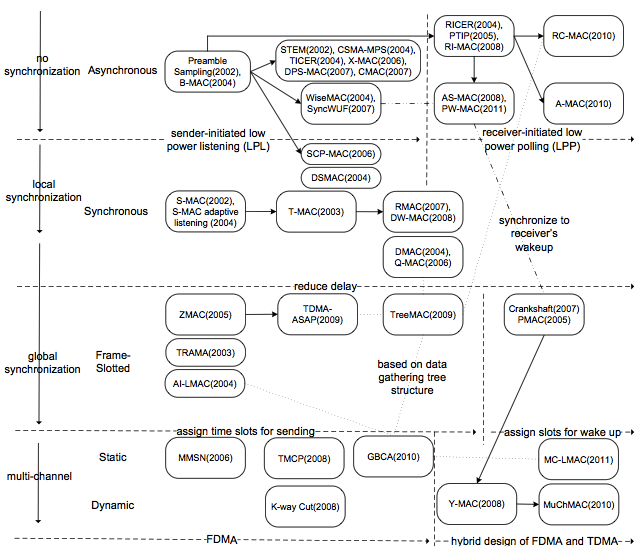
\includegraphics[width=12.5cm]{images/ch3-taxonomie-mac.png}
\flcaption{Taxonomie des différents protocoles MAC conçus pour
les réseaux de capteurs sans-fil (travaux académiques).
Source~: \cite{Evolution-MAC-WSN-Survey-2013}}
\label{FigTaxonomieMAC}
\end{figure}

Pour le moment, et malgré tous ces développements, les protocoles
asynchrones LPL restent, du moins dans le milieu académique, les plus
couramment utilisés. Ils sont en effet bien adaptés aux trafics réseaux
modérés, ce qui correspond au mode de fonctionnement de la majorité des
réseaux de capteurs sans-fil à l'heure actuelle, et permettent à la fois
une bonne économie des ressources, tant du point de vue énergétique
(économie de la batterie des noeuds) que matériel (simplicité
d'implantation, d'où une faible occupation de la mémoire~--- d'une
capacité souvent extrêmement limitée~--- de ces appareils).
Le protocole ContikiMAC, grâce à la forte influence du système
d'exploitation Contiki dans le domaine des réseaux de capteurs
sans-fil (comme nous allons le voir dans la section \vref{SecOSWSN})
tend actuellement à devenir le standard de fait dans les différents
travaux de recherche dans le domaine.

Toutefois, l'adoption de l'amendement 802.15.4e au standard IEEE,
avec sa couche MAC évoluée (mécanisme TSCH) et le développement d'une
pile réseau complète sur cette base (projet 6TiSCH \cite{6TiSCH}
\cite{6TiSCHbis} \cite{6TiSCHter}) pourraient prochainement changer
la donne, et imposer un nouveau standard notamment dans les réseaux
industriels exigeants~--- surtout ceux composés de noeuds puissants
pouvant jouer le rôle de FFD (\lang{``Full Function Devices''}).
Le développement de la pile réseau avancée OpenWSN est un autre facteur
susceptible de faciliter une telle évolution.


%%%%%%%%%%%%%%%%%%%%%%%%%%%%%%%%%%%%%%%%%%%%%%%%%%%%%%%%%%%%%%%%%%%%%%%%%%%%%

\section{Systèmes d'exploitation dédiés}
\label{SecOSWSN}

Des systèmes d'exploitation spécialisés pour les appareils embarqués
spécifiques que sont les noeuds des réseaux de capteurs sans-fils
(les \lang{``motes''}) ont été conçus et publiés depuis maintenant
plus d'une dizaine d'années.

Rappelons que pour des raisons juridiques aussi bien que techniques~---
possibilité de modifier et d'améliorer le c{\oe}ur et les différents
composants du système selon nos besoins~--- nous n'avons étudié et
envisagé l'utilisation que des systèmes à licence libre et \lang{open
source}.

\subsection{Rappels sur les notions de multi-tâche}
\label{SubsecMultitache}

\`A un moment donné, un micro-contrôleur (du moins la majorité d'entre eux,
qui ne disposent que d'un unique <<~c{\oe}ur~>>) ne peut exécuter qu'une
tâche à la fois. Pour qu'un système informatique, comme une \lang{mote},
puisse effectuer plusieurs tâches, il est nécessaire de passer régulièrement
et très rapidement d'une de ces tâches à une autre. Cela introduit la notion
de \emph{changement de contexte}~: lorsqu'on passe d'une tâche A à une
autre tâche B, on sauvegarde l'état de A pour charger celui de B~;
l'état d'une tâche étant nommé son \nom{contexte} (il s'agit des valeurs
des registres du processeur, des périphériques, etc.)

L'espace où sont sauvegardés les contextes des différentes tâches est nommé
\emph{pile} (en anglais~: \lang{``stack''}). Il s'agit d'une structure
de données variable située en mémoire (RAM donc), suivant le paradigme
<<~dernier entré, premier sorti~>> (en anglais LIFO~: \lang{Last In
First Out}).

Notons que la pile n'est pas dédiée aux seuls contextes de tâches~:
elle sert également de zone de travail en mémoire pour les programmes
en cours d'exécution (variables locales, appels de sous-programmes, etc.)

Selon la conception du système d'exploitation, il peut y avoir une seule
pile commune à tout le système, ou plusieurs piles dédiées aux différentes
tâches, comme nous allons le voir.

On distingue deux principaux modèles conceptuels pour réaliser un système
multi-tâche~:

\begin{description}

\item[le multi-tâche coopératif~:] dans ce modèle, chaque tâche doit prévoir
explicitement dans son  code source de <<~passer la main~>> (par l'appel à
une fonction dédiée du système d'exploitation).
Ce modèle rend les systèmes d'exploitation plus simples à concevoir et
plus compacts~: il est en effet possible dans ce cas d'employer une pile
unique pour l'ensemble du système.
En contrepartie, la programmation d'applications est plus contraignante~:
le développeur doit gérer lui-même le basculement d'une tâche à une autre,
sinon le système est condamné à mal fonctionner, et même en général à se
bloquer (<<~se planter~>>). Ce modèle rend donc au final le système moins
robuste~: une tâche mal programmée (par exemple~: ne passant pas la main)
peut mettre tout le système hors service.

\item[le multi-tâche préemptif~:] dans ce modèle, le système d'exploitation
alloue lui-même les intervalles d'exécution à chaque tâche, et planifie
automatiquement les changements de contexte entre celles-ci (cette capacité
d'interrompre une tâche sans collaboration de sa part est nommée
\nom{préemption}). Ce modèle implique des systèmes d'exploitation plus
évolués et gourmands en ressources~: il est en effet nécessaire d'avoir une
pile distincte par tâche. En contrepartie, la programmation d'applications
est nettement simplifiée~: le développeur n'a pas à se soucier des
changements de tâches. Le système est en outre nettement plus robuste~:
une tâche « bloquée » ne va pas systématiquement mettre hors service
tout le système.

En outre, la capacité d'interrompre à n'importe quel moment une tâche
en cours est un pré-requis pour implanter un système temps réel, qui
a besoin de pouvoir réagir à un évènement comme une interruption en un délai
limité. C'est pourquoi les systèmes offrant des fonctionnalités temps-réel
sont basés sur le modèle préemptif, le multi-tâche coopératif~---
qui oblige à attendre que la tâche en cours soit prête à passer la main~---
étant par conception défavorable à ces fonctionnalités.\\
Cela est illustré par la figure \vref{FigModeleMultitache}.
On notera notamment la latence présente en modèle coopératif \textbf{A}
due à l'attente de la fin de la tâche en cours, absente du modèle préemptif
\textbf{B} pouvant interrompre une tâche à tout moment (sauf à être
déjà en train de gérer un évènement ou une interruption).

\end{description}

\begin{figure}[!hbt]
\centering
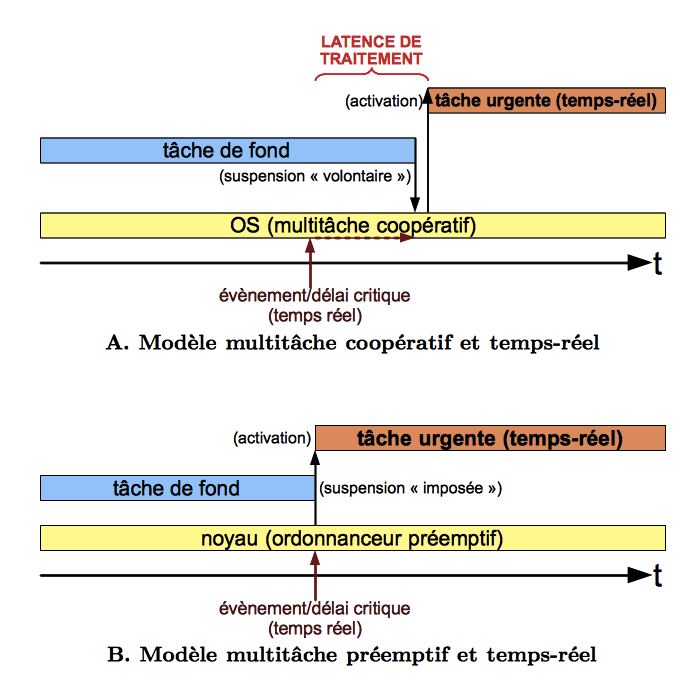
\includegraphics[width=12.75cm]{images/ch3-modeles-multitache.png}
\flcaption{Principe de base du traitement des évènements temps-réel par
les diférents modèles de gestion multi-tâche.}
\label{FigModeleMultitache}
\end{figure}


\subsection{TinyOS}
\label{SubsecTinyOS}

Le premier système ayant connu un large succès dans le domaine des réseaux
de capteurs sans-fil est \nom{TinyOS} \cite{TinyOS}. Il s'agit d'un système
\lang{open-source} et libre (sous license BSD), dont la première version
stable (version 1.0) a été publiée en septembre 2002. Il est extrêmement
léger, et par là-même très bien adapté aux appareils limités que sont
les noeuds des réseaux de capteurs sans-fil de la première génération
(Mica2, MicaZ \cite{DSMicaZ}, TelosB~/ SkyMote \cite{DSTelosB}, etc.).

Ce système a permis de nombreuses avancées dans le domaine, comme la
possibilité d'utiliser le protocole réseau Internet (IP, y compris dans
sa dernière version~: IPv6) ainsi que des protocoles de routage (comme
RPL) sur les réseaux au standard IEEE 802.15.4. Il a également introduit
la possibilité de simuler des réseaux de \lang{motes} fonctionnant sous
TinyOS, grâce au simulateur \nom{TOSSIM} \cite{TOSSIM}.

L'un des principaux défauts de ce système est la nécessité d'apprendre
un langage spécifique~--- nommé \nom{nesC} \cite{nesC}~--- pour pouvoir
travailler et développer des applications avec TinyOS. Contrairement à
ce que son nom pourrait laisser penser, le langage nesC est très différent
du langage C classique et de tous les autres langages informatiques
impératifs couramment utilisés~--- il ressemble plutôt, dans sa philosophie,
aux langages de description de matériel utilisés dans la conception de
circuits intégrés, comme VHDL ou Verilog. En cela, il peut se révéler
difficile à apprendre et à maîtriser pour des programmeurs ayant une
formation de développement informatique classique.

La présence de ce langage spécifique au sein du projet TinyOS n'est pas
un hasard~: TinyOS est en effet construit sur ses propres paradigmes
spécifiques. Ce système gère les entrées~/ sorties (I/O) de façon
totalement asynchrone, et fonctionne autour d'une pile unique, depuis
laquelle les différents composants constituant une application TinyOS
sont appelés en tant que \lang{callbacks} statiquement liés. 
TinyOS a en effet été conçu pour fonctionner de façon principalement
évènementielle, via la programmation de gestionnaires d'interruptions.

La notion de <<~tâche~>> de longue durée existe, mais la gestion du
multitâche est sous TinyOS particulièrement limitée~: les <<~tâches~>>
sont exécutées l'une après l'autre, suivant une file (FIFO) dont l'ordre
ne peut être modifié~--- l'ordonnanceur de TinyOS n'est pas conçu
pour changer dynamiquement l'ordre des tâches à exécuter en fonction
du déroulement de l'application et de son environnement. Les tâches
ne peuvent en outre être préemptées que par des interruptions
(<<~évènements~>>) mais jamais par d'autres tâches. Le manuel
de TinyOS définit en fait les tâches comme des appels de procédures
différés (\lang{``Deferred Procedure Calls''}). Ce fonctionnement
permet toutefois de minimiser grandement la consommation d'énergie,
toute la \lang{mote} étant en sommeil lorsqu'aucune tâche n'a à
s'exécuter (le prochain réveil étant provoqué par <<~l'évènement~>>
suivant).

Il est clair que le fonctionnement de TinyOS et ses paradigmes sont
particulièrement atypiques par rapport aux autres systèmes décrits
dans la présente section. Ceci se ressent dans la programmation
d'applications, qui nécessite de maîtriser ces notions pour savoir
décomposer tout programme en divers <<~évènements~>>, <<~tâches~>> et
autres <<~commandes~>> (appel d'un composant à un autre) pour créer
les composants constituant les applications.
La difficulté d'apprentissage et de maîtrise de ce système pour un
informaticien formé et habitué aux notions classiques de programmation
sera ainsi assez ardue.

L'ensemble des architectures matérielles sur lesquelles TinyOS a été porté
semble actuellement se limiter aux familles AVR et MSP430 (un portage sur
des architectures plus puissantes comme les Cortex-M est évoqué dans la
FAQ du site Web de TinyOS, mais son état d'avancement actuel est inconnu).

Enfin, signalons que TinyOS nécessite l'emploi d'outils de développement
dédiés (langage spécifique oblige) pour pouvoir être compilé.

Toutes ces limitations, ajoutées à un rythme de développement relativement
lent~--- la dernière version stable (2.1.2) remonte à août 2012~--- ont
ces dernières années nui à son adoption, et il n'est désormais plus
le système de référence ni le plus utilisé dans le domaine des réseaux
de capteurs sans-fil.


\subsection{Contiki}
\label{SubsecContikiOS}

Le système d'exploitation de référence dans le domaine des réseaux de
capteurs sans-fil et par extension de l'Internet des objets (IoT) est
\nom{Contiki} \cite{ContikiOS}. Il s'agit également d'un système
\lang{open source} et libre (license BSD), dont la première version
publiée remonte à 2002. Le projet Contiki a été à l'origine de nombreuses
avancées~: on pourra citer entre autres la pile TCP/IP embarquée \nom{uIP}
\cite{uip} depuis étendue en \nom{uIPv6} (qui est présentée comme la pile
IPv6 fonctionnelle la plus légère qui soit), la pile réseau \nom{Rime}
\cite{Rime} simplifiée et orientée vers les économies d'énergie,
ou encore le simulateur avancé de réseaux de capteurs sans-fil
\nom{Cooja} \cite{Cooja}.

S'il est légèrement plus exigeant en ressources que TinyOS, Contiki
reste très léger et particulièrement bien adapté aux \lang{motes}
constituant les réseaux de capteurs sans-fil.

Son principal avantage sur TinyOS est d'être basé sur des paradigmes
standards, avec une API reprenant les principes classiquement rencontrés
dans le domaine des systèmes d'exploitation~; il est en outre codé en
langage C standard~: ceci rend son apprentissage et sa maîtrise bien plus
facile pour un programmeur ayant un cursus classique.

Contiki est basé sur un noyau événementiel, implantant un modèle
multitâche coopératif. Il offre également une pile réseau complète,
directement prête à l'emploi.

Il a été porté sur une multitude de plate-formes, comprenant de nombreuses
\lang{motes} pour réseaux de capteurs sans-fil, mais aussi de vieux modèles
d'ordinateurs personnels~--- Commodore~64, Apple~II, Atari~800XL...~---
et même certains modèles de consoles de jeux (dans des portages
non-officiels).

Des modules optionnels permettent également de fournir des fonctionnalités
aussi diverses qu'une interface graphique, un système de fichiers, ou
encore une mise à jour du programme (\lang{``firmware''}) durant
l'exécution (suivant un processus certes complexe).

Toutes ces caractéristiques et avantages ont largement contribué à la
diffusion et à l'adoption massive de Contiki, ce qui fait qu'il s'agit
désormais du système d'exploitation de référence dans le monde des
réseaux de capteurs sans-fil.

Les développeurs de Contiki ont également été actifs quant au développement
de la couche MAC/RDC~: nombre de protocoles classiques (comme par exemple
X-MAC) ont été implantés dans la pile réseau de ce système~; et un nouveau
protocole, ContikiMAC \cite{ContikiMAC}, a été spécifiquement conçu pour
jouer le rôle de protocole RDC par défaut de Contiki (en collaboration avec
le protocole CSMA/CA du standard IEEE 802.15.4 en tant que couche MAC).
Nous avons abordé ce protocole ContikiMAC dans l'étude des protocoles
LPL plus haut en section \vref{ParContikiMAC}.

Toutefois, la compacité de Contiki, son optimisation et ses fonctionnalités
imposent en contrepartie diverses limitations à ce système.

Contiki est basé sur un modèle multitâche coopératif, et non préemptif~:
l'ordonnanceur de tâches se déclenche en réaction à des <<~évènements~>>
(pour reprendre la terminologie de Contiki). Cet ordonnanceur ne peut se
déclencher que selon un rythme spécifique, dont la fréquence (intervalle
de déclenchement) est déterminée à la compilation. Ce modèle de
fonctionnement multitâche est, comme nous l'avons vu ci-dessus en section
\vref{SubsecMultitache}, un obstacle à la présence de fonctionnalités
temps-réel.

Il faut en outre noter que l'ordonnanceur coopératif de Contiki est
conçu pour traiter un type spécifique de tâches nommé \nom{protothreads}
\cite{Protothreads}. Ce mécanisme permet de gérer différentes files
d'exécution (\lang{``threads''}) sans avoir besoin de maintenir
une pile d'exécution séparée pour chacun d'entre eux.
Le grand avantage de cette technique est la possibilité d'utiliser une pile
unique pour tout un système, diminuant ainsi significativement la quantité
de RAM nécessaire, sans pour autant devoir se limiter à un mécanisme
d'ordonnancement statique comme dans TinyOS.
Ce mécanisme de \lang{protothreads} est d'ailleurs utilisé dans
plusieurs autres applications en dehors de Contiki.
La contrepartie de ce mécanisme est qu'il est nécessaire de respecter
certaines règles rigoureuses quant à l'utilisation de certains éléments
du langage C~: il est notamment impossible d'utiliser l'instruction
\texttt{switch} dans certaines parties d'un programme utilisant ces
\lang{protothreads}.

Toutes ces limitations du système Contiki ont posé des problèmes
non résolus pour nos travaux de thèse, comme nous le verrons dans
la section \vref{SecLimContiki} du présent manuscrit.


\subsection{Nano-RK}
\label{SubsecNanoRK}

Un système spécialisé dans les réseaux de capteurs sans-fil présentant
des propriétés très intéressantes, et surtout proches de nos besoins, est
\nom{Nano-RK} \cite{NanoRK}. Il a été conçu à l'Université de Carnegie
Mellon à partir de 2005.

Il s'agit également d'un système \lang{open source}, publié selon un schéma
de double licence permettant l'utilisation de la GNU GPL (\lang{General
Public License}) si tel est le choix du développeur. On peut donc le
considérer comme un logiciel libre.

Celui-ci fournit de nombreuses fonctionnalités intéressantes~:

\begin{itemize}

\item Un noyau fonctionnant en mode \emph{tickless} (c'est-à-dire sans
nécessiter un \lang{timer} le déclenchant de façon régulière).

\item Un \emph{ordonnanceur temps-réel} avec \emph{multi-tâche préemptif
gérant les priorités}.\\
La granularité théorique~--- permettant de descendre jusqu'à la nano-seconde
par l'utilisation de la représentation temporelle POSIX, réimplantée sous
le nom de \texttt{nrk\_time\_t}~--- est excellente. Mais en pratique, la
granularité effective garantie pour les interruptions (\lang{``timer
tick''}) est de l'ordre de la milliseconde \cite{NanoRKTimeMgt}.
Cela implique une gigue (\lang{``jitter''}) pouvant aller jusqu'à
1000~microsecondes, alors que la durée de base d'une période de
\lang{backoff} CSMA/CA est de seulement 320~microsecondes.
Les fonctionnalités temps-réel de Nano-RK, aussi avancées et complètes
soient-elles, offrent donc une granularité pouvant ne pas être suffisante
pour nos travaux.

\item Un paradigme de \emph{réservations de ressources } très intéressant,
permettant par exemple d'accorder respectivement 100 ms de temps d'exécution
ou l'envoi de 10 paquets par seconde pour une tâche ou un noeud donnés.
Il s'agit en fait d'un principe de quotas, assuré par le noyau système,
et permettant de prévoir un <<~budget énergétique~>> consommé par un
appareil donné pendant une période de temps. Il s'agit d'une spécificité
très avancée et fonctionnellement très prometteuse de Nano-RK.

\item Une occupation mémoire réduite (bien que légèrement supérieure
à celle de TinyOS ou Contiki).

\item Une gestion intégrée des erreurs fatales (violations d'espace
mémoire ou de \lang{timing}, \lang{watchdog}, chutes d'alimentation
énergétique...)

\item Le système est écrit en langage C standard, et est donc compilable
avec le compilateur GNU GCC classique.

\item Une pile réseau légère, comprenant notamment plusieurs protocoles
MAC classiques, dont le protocole LPL B-MAC (voir section
\vref{ParBMAC})~; d'autres protocoles spécifiques et expérimentaux
sont proposés, ainsi qu'une fonction simple de passerelle vers
un réseau IP nommée \lang{``SLIPStream''}.

\end{itemize}

Ce système a le principal désavantage d'avoir été porté sur un nombre limité
d'architectures de microcontrôleurs~: seules les plates-formes MSP430 et AVR
sont supportées, avec une activité et une spécialisation nettement plus
grandes vis-à-vis de cette dernière. Les principales plates-formes
matérielles sur lesquelles Nano-RK est employé sont en effet~:
\begin{itemize}

\item la \lang{``mote''} MICAz \cite{DSMicaZ}, de conception déjà ancienne
(contemporaine de la TelosB/SkyMote) basée sur un MCU ATmega128L
\cite{DSATmega128L} et le classique TI CC2420 \cite{DSCC2420} comme radio~;

\item la plus récente FireFly3 \cite{FireFly3}, spécifiquement conçue
par Carnegie Mellon pour servir de plate-forme matérielle à Nano-RK.
Elle a la particularité d'être conçue autour d'un microcontrôleur intégrant
un émetteur~/ récepteur radio, l'ATmega128RFA1 \cite{DSATmega128RFA1},
et peut accueillir plusieurs cartes d'extension, notamment une carte
comportant de nombreux capteurs (température, pression, humidité,
accéléromètre, audio, mouvement...).

\end{itemize}

Ces deux \lang{``motes''}, mises en avant sur le site de Nano-RK, sont
toutes deux basées sur l'architecture Atmel AVR. Si cela peut présenter
certains avantages~--- comme la possibilité, mise en avant par le projet,
de développer et déboguer directement Nano-RK avec l'outil Atmel Studio~---
cela implique une forte limitation au niveau de la portabilité, laquelle
est pourtant l'un des principaux objectifs recherchés en utilisant un
système d'exploitation pour développer sur WSN.

Aucune activité de portage sur d'autres matériels ou architectures ne
semble entreprise~: cela est fort regrettable, sachant que les
\lang{``motes''} basées sur des microcontrôleurs 32 bits (comme ceux
d'architecture ARM), plus puissantes, apparaissent et se répandent
de plus en plus.

Cela n'empêche toutefois pas Nano-RK d'être encore activement développé
(bien qu'avec des moyens humains visiblement limités, comme beaucoup de
projets strictement académiques), et de faire régulièrement l'objet
de publications, citons par exemple \cite{NanoRKHW2013}.

Toutefois, malgré ces qualités, nous n'avons pas dans le cadre de cette
thèse travaillé avec Nano-RK, car nous avons été amenés à découvrir une
autre plate-forme logicielle très intéressante et plus ouverte.
Nous allons maintenant aborder cette plate-forme dans la section
\ref{SubsecRIOTOS} ci-dessous.


\subsection{RIOT OS}
\label{SubsecRIOTOS}

Nous avons été amenés à nous intéresser, dans le cadre de nos travaux
de thèse, à \nom{RIOT OS} \cite{RIOT}.

Ce nouveau système~--- sa première version a été publiée en 2013~---
est également \lang{open source} et publié sous une licence libre
(LGPL v2.1), et est spécifiquement conçu pour les noeuds de réseaux
de capteurs sans-fil.

Il est développé principalement avec le soutien de la
\lang{Freie Universität Berlin}, de l'INRIA, et de la
\lang{Hamburg University of Applied Sciences}. Il est à noter que
l'équipe de développement de ce projet est particulièrement accueillante
et ouverte aux contributions extérieures.

\medskip

Il fournit les avantages de base que l'on peut attendre d'un OS pour
réseaux de capteurs sans-fil, notamment la portabilité (il fonctionne
sur de nombreux appareils reposant sur les architectures MSP430, AVR et
ARM~--- notamment la famille des Cortex-M), ainsi qu'un ensemble complet
de fonctionnalités, notamment une pile réseau.

Parmi les fonctionnalités offertes, on retrouve de nombreuses capacités
avancées des autres OS spécialisés dans les capteurs sans-fil (comme
Nano-RK), plus d'autres \lang{a priori} inédites~:

\begin{itemize}

\item Un \emph{micro-noyau} léger, dirigé par les interruptions,
fonctionnant par défaut de façon \lang{tickless} (c'est-à-dire sans
nécessiter qu'un \lang{timer} le déclenche de façon régulière).

\item Un ordonnanceur, intégré au micro-noyau, fonctionnant en mode
\emph{multi-tâche préemptif avec gestion des priorités}.

\item Une utilisation optimisée des \emph{timers matériels grâce à une
API dédiée}, permettant de programmer le déclenchement d'actions avec
une granularité très fine, de l'ordre de la dizaine de microsecondes.

\item Des structures de données de base~: piles, files, listes
chaînées et circulaires.

\item Des mécanismes de communication entre tâches (\lang{threads)}~:
notamment un système de passage de messages~--- implanté par l'utilisation
de queues (FIFO) de messages, appartenant chacune à un \lang{thread}
donné~---, ainsi que des \lang{mutex}.

\item RIOT est entièrement écrit en \emph{langage C standard}~;
de plus, contrairement à Contiki, il n'y a aucune restriction quant
aux éléments utilisables du langage (telles que les limitations
imposées par les \lang{protothreads}).

\item Une conception claire et modulaire, rendant le développement
avec mais aussi \emph{dans} le système plus facile et productive.

\item Une gestion des erreurs critiques, que nous avons dans le cadre
de cette thèse initiée et contribué à mettre en place.

\end{itemize}

Les trois premières fonctionnalités citées ci-dessus font de RIOT
un système \emph{temps-réel} à part entière.

\bigskip

Notons que le mécanisme de gestion des \lang{timers} matériels a évolué
pendant l'année 2015. L'ancien mécanisme \texttt{hwtimer}, qui était intégré
au noyau lui-même, a été supprimé et remplacé par un module nommé
\texttt{xtimer}.

Toutes les expériences décrites dans ce manuscrit ont, sauf indication
contraire, été basées sur une version de RIOT utilisant l'ancien système
\texttt{hwtimer} intégré au noyau. Celui-ci a été conçu pour offrir
la possibilité d'utiliser les \lang{timers} matériels du microcontrôleur,
et ce avec une granularité aussi fine que le permettent les \lang{``ticks''}
de ces \lang{timers}. Sur les premières \lang{motes} que nous avons utilisé
(voir section \vref{SecHWMSP430}), nous avons ainsi disposé d'une granularité
d'environ $30,5~\mu$s pour programmer le déclenchement de nos évènements.

\medskip

Le nouveau module \texttt{xtimer} permet lui de s'abstraire de la notion
de \lang{``tick''}, c'est à dire du délai (en général fixe) entre deux
déclenchements successifs d'un \lang{timer} matériel, pour proposer des
délais exprimés systématiquement en microsecondes, le module \texttt{xtimer}
étant conçu pour être implanté sur la base d'un timer matériel dont la
cadence est fixée à 1~MHz. Cette implantation lui permet donc d'atteindre,
en théorie, une granularité à la microseconde près~; dans les faits,
les délais d'exécution des fonctions mêmes de \texttt{xtimer}, ainsi que
la possibilité de préemption par le noyau (hors gestionnaire d'interruption)
génèrent une gigue allant jusqu'à quelques dizaines de microsecondes, soit
(dans les cas les moins favorables) une granularité comparable
à celle offerte par le mécanisme précédent.

Notons quoi qu'il en soit que la disponibilité en standard d'une granularité
temporelle, pour les mécanismes temps-réel de RIOT, de l'ordre de la dizaine
de microsecondes (c'est-à-dire largement inférieure à la milliseconde) 
est une fonctionnalité exceptionnelle~: nous ne l'avons retrouvée lors
de nos recherches dans aucun autre OS dédié aux WSN (par exemple, dans
Nano-RK \cite{NanoRKTimeMgt} qui dispose pourtant d'un mécanisme de
\lang{timing} évolué). Même FreeRTOS (cf. section \vref{SubsecFreeRTOS})
n'offre par défaut qu'un mécanisme de \lang{software timer} d'une granularité
d'1~ms, l'utilisation des potentialités des \lang{timers} matériels étant
laissée à la seule charge du développeur d'applications
\cite{FreeRTOSTimerRes}.

Le fonctionnement \lang{tickless} du noyau et l'utilisation optimale
des \lang{timers} matériels font également de RIOT OS une plate-forme
logicielle prometteuse pour le développement d'applications particulièrement
optimisées et économes en énergie, ces deux fonctionnalités permettant
potentiellement de garder le MCU en état de <<~sommeil~>> (basse
consommation) durant une fraction de temps aussi élevée que possible.
Nano-RK a déjà exploré la piste du fonctionnement \lang{tickless} pour
augmenter son efficacité énergétique (voir \cite{NanoRKTimeMgt}).

\medskip

Un des désavantages de RIOT, par rapport à TinyOS et Contiki, est sa
plus grande exigence en ressources matérielles, notamment concernant
l'occupation mémoire. La pile réseau complète (de la couche physique
à l'implantation 6LoWPAN en passant par les couches RPL et MAC~/ RDC)
ne peut pas être compilée pour un matériel de type SkyMote~/ TelosB
car la quantité de mémoire exigée dépasse celle disponible sur ces
appareils. À l'heure actuelle, des noeuds limités comme ceux basés
sur l'architecture MSP430 sont cantonnés sous RIOT au rôle de RFD,
les rôles de FFD étant pour l'instant réservés aux matériels plus
puissants (comme ceux basés sur des microcontrôleurs ARM).

Notons toutefois que, grâce à l'architecture modulaire du système,
le noyau RIOT compilé avec les seules couches PHY et MAC~/ RDC reste
très léger et occupe très peu de mémoire, étant ainsi parfaitement
compatible même avec les appareils les plus limités. 

En outre, la partie réseau du système ayant fait l'objet d'une
réorganisation en profondeur (comme nous le verrons plus en détail
ultérieurement en section \vref{SecGnrcRIOT}), nous espérons qu'à
l'avenir, il sera possible d'utiliser encore plus efficacement
des appareils aux ressources limitées sous RIOT.

\medskip

Notons également qu'outre la pile réseau intégrée de RIOT, la pile
\nom{OpenWSN} \cite{OpenWSN} a fait l'objet d'un portage sur le noyau
RIOT. Ce dernier est donc l'une des deux plates-formes logicielles
sélectionnées pour accueillir cette pile à hautes performances (l'autre
étant le noyau FreeRTOS \cite{FreeRTOS}). 


\subsection{Autres OS spécialisés}
\label{SubsecAutresOS}

D'autres systèmes d'exploitation spécifiquement conçus pour les réseaux
de capteurs sans-fil ont été développés, mais ceux-ci sont nettement
moins utilisés, et souffrent de limitations nous ayant empêché 
d'envisager sérieusement leur utilisation.

\begin{description}

\item[SOS] \cite{SOS}
Le développement de ce système a été arrêté en novembre 2008. Ses auteurs
recommandent explicitement sur leur site Web de <<~considérer l'utilisation
d'alternatives activement maintenues.~>>

\item[Lorien] \cite{LorienOS}
Si celui-ci est basé sur approche orientée composant intéressante,
ce système ne semble pas d'une utilisation très répandue. Il n'est
actuellement disponible que pour un seul type de matériel (TelosB~/
SkyMote) ce qui limite considérablement la portabilité que l'on est
en droit d'attendre de l'utilisation d'un OS, donc son intérêt.
En outre, son développement semble avoir nettement ralenti,
la dernière version stable publiée par le projet Lorien datant de 2011,
tandis que le dernier \lang{commit} dans le dépôt SourceForge du
projet (r46) remonte à janvier 2013.

\item[Mantis] \cite{MantisOS}
Alors que ce projet prétend être \lang{open source}, celui-ci n'a
publié aucune version accessible sur son site SourceForge~; en outre,
l'accès au dépôt source du projet
(\texttt{http://mantis.cs.colorado.edu/viewcvs}) semble défaillant.
Enfin, les dernières nouvelles officielles affichées sur la page Web
principale du projet parlent d'une version bêta censée être publiée en 2007.
Les dernières publications scientifiques concernant MantisOS semblent
également remonter à l'année 2007. Tous ces éléments nous font penser
que ce projet est tombé à l'abandon...

\item[LiteOS] \cite{LiteOS}
Ce système offre des fonctionnalités très intéressantes, notamment
la possibilité de mettre à jour le \lang{firmware} des noeuds à la
volée, depuis la connexion réseau sans-fil (mise à jour
\lang{``Over-the-Air''}, dont LiteOS semble avoir été le pionnier),
ainsi que le support intégré d'un système de fichiers hiérarchique.
Malheureusement, LiteOS est actuellement uniquement disponible pour
les plates-formes matérielles IRIS et MicaZ, et nécessite l'emploi
d'Atmel Studio pour son développement. Cela nuit gravement à la
portabilité du système, vu que LiteOS semble très fortement lié
à l'architecture de microcontrôleurs AVR.

\item[MansOS] \cite{MansOS}
Ce système très récent offre de nombreuses fonctionnalités
intéressantes, comme le multi-tâche préemptif (de façon optionnelle),
une pile réseau intégrée, et un langage de script. Il est disponible
sur deux architectures de microcontrôleurs~: AVR et MSP430 (mais
malheureusement, pas les architectures ARM dont la progression est
constante). En outre, les capacités temps-réel du système semblent
limitées~: seuls des \lang{timers} logiciels d'une granularité
minimale de 1~milliseconde semblent disponibles.

\item[NanoQplus] \cite{NanoQplus2008}
Il s'agit d'un système dédié aux WSN, apparu semble-t-il en 2008,
annonçant des fonctionnalités intéressantes comme le multitâche
préemptif, une grande portabilité sur de nombreuses architectures de MCUs
(allant des 8~bits aux 32~bits), et surtout un système de protection mémoire.
L'article de 2008 le présentant \cite{NanoQplus2008} semble prometteur, et
un autre article de 2011 \cite{NanoQplusIPv6RPL2011} indique qu'une pile
IPv6 ainsi que RPL y ont été portés.\\
Malheureusement, le site du projet
(\texttt{http://dukemon.tistory.com/tag/NanoQplus}) est exclusivement
en coréen, et seul un faible nombre d'articles écrits en Corée (le plus
souvent en coréen) semblent y faire référence~--- les deux publications
citées dans le présent paragraphe, certes en anglais, sont parues dans
des journaux~/ évènements se voulant internationaux mais s'étant déroulés
en Corée.\\
Il semble donc malheureusement difficile de se faire une idée précise
de ce système, dont l'adoption hors de son pays d'origine semble
actuellement extrêmement limitée.

\item[OpenTag]
Il s'agit d'une pile réseau chargée d'implanter le protocole
DASH7 (standard ISO/IEC 18000-7, spécialisé dans le RFID et incompatible
avec le standard IEEE 802.15.4), fournie avec son propre système
temps-réel minimaliste (noyau dédié). S'il s'agit \lang{stricto sensu}
d'un système fonctionnant sur des WSN, lesdits WSN sont très différents
de ceux que nous étudions dans cette thèse~--- ils fonctionnent par
exemple à la fréquence radio de 433~MHz réservée à DASH7. Leur
développement a au départ été prévu pour des applications militaires.
Il ne s'agit donc pas d'un système comparable à tous ceux que nous
avons vu jusqu'à présent, et ne correspond absolument pas aux travaux
de notre thèse.

\end{description}


\subsection{OS temps-réel classiques~/ généralistes}
\label{SubsecOSTempsReel}

Une autre possibilité utilisée par plusieurs constructeurs de
\lang{motes} est de recourir à des systèmes embarqués <<~classiques~>>,
lesquels offrent le plus souvent des fonctionnalités temps-réel.

\subsubsection{FreeRTOS}
\label{SubsecFreeRTOS}

\hyphenation{Free-RTOS}

La référence actuelle en matière de système d'exploitation temps-réel
\lang{open source} pour l'embarqué est \nom{FreeRTOS} \cite{FreeRTOS}.

FreeRTOS est un projet mature (première version publiée en 2003),
stable et très largement employé, notamment dans l'industrie.

Il a été porté sur plus de 30 architectures de microcontrôleurs différentes,
c'est-à-dire quasiment toutes les architectures présentes sur le marché~;
ce qui en fait le système le plus portable cité jusqu'ici dans le présent
manuscrit, largement devant n'importe quel système dédié aux réseaux de
capteurs sans-fil.

L'un des points forts majeurs de FreeRTOS est son excellente documentation~:
le code source est abondamment et consciencieusement commenté, et l'auteur
publie deux manuels complets (en anglais uniquement) sur son système~:
\begin{enumerate}
\item un manuel d'utilisation \cite{FreeRTOSTuto}, complet et très
didactique, tant sur l'utilisation du système lui-même que sur les notions
de temps-réel en informatique et les conséquences de ces notions quant aux
bonnes pratiques de programmation~;
\item un manuel de référence du système \cite{FreeRTOSRef}, détaillant
de façon exhaustive l'API et les options de configuration, avec de
nombreux exemples de code (\lang{``listings''}).
\end{enumerate}
Ces deux ouvrages, rédigés avec soin et maintenus à jour, facilitent
considérablement l'apprentissage et la programmation avec ce système.
Il s'agit également d'une des sources de revenus du projet FreeRTOS,
ces deux manuels étant vendus sous forme électronique sur le site
Web du projet~: cette documentation sur FreeRTOS n'est donc
\emph{pas} libre, contrairement au système lui-même qui est publié
sous la licence GNU GPL.

Le code source du noyau en lui-même se compose uniquement de quatre fichiers
source en langage C~--- dont un représente une fonction optionnelle
(coroutines). Le reste du source du projet se compose des portages (couches
d'abstraction) pour les nombreuses plates-formes matérielles et compilateurs
supportés, et d'exemples. Ce système reste ainsi très léger quant aux
ressources matérielles exigées (généralement moins de 10~Ko de code
programme) ce qui le rend parfaitement adapté aux systèmes embarqués
les plus limités.

La simplicité du noyau (quantité de code minimale) et les critères de
qualité stricts imposés au code source contribuent à la robustesse
de FreeRTOS.

Cela lui permet d'ailleurs de fournir une version certifiée
pour les utilisations dans les systèmes embarqués critiques, nommée
\nom{SafeRTOS}. Contrairement au noyau FreeRTOS de base, SafeRTOS
n'est \emph{pas} un logiciel libre~: l'achat d'une licence payante est
exigé, en échange de la certification (IEC 61508: SIL 3) et d'un support
technique avancé. Cette version spéciale, SafeRTOS, est une autre source de
revenus du projet FreeRTOS (en plus de la vente de manuels citée plus haut).

Citons également l'existence d'\nom{OpenRTOS}, qui est un clone absolu
de FreeRTOS sous une licence \emph{propriétaire}, vendu à l'intention des
industriels rebutés par les exigences de la GNU GPL, et fournissant
également un support technique~--- et par la même occasion une troisième
source de revenus au projet FreeRTOS.

\medskip

Le noyau FreeRTOS fournit des fonctionnalités avancées telles que~:
\begin{itemize}
\item le multi-tâche, préemptif par défaut, coopératif en option,
via un ordonnanceur gérant les priorités~;
\item un mode \lang{``tickless''} optionnel~;
\item des structures de données de base (listes, files)~;
\item des mécanismes de communication entre tâches (\lang{``Inter Process
Communication''})~: sémaphores, \lang{mutex}~;
\item des \lang{timers} logiciels~;
\item et une gestion optionnelle de l'allocation de mémoire
(\lang{``heap''})~: trois mécanismes différents disponibles.
\end{itemize}

Cette compacité a toutefois un prix~: FreeRTOS n'est en fait qu'un
noyau, fournissant les fonctionnalités de base citées ci-dessus.
Il est dépourvu de tout pilote matériel, y compris pour les périphériques
de base intégrés aux microcontrôleurs (par exemple~: les ports séries ou
les GPIO)~--- ces pilotes de périphériques devant être développés et
fournis en sus par les fournisseurs de matériels et~/ ou d'applications
désireux de l'utiliser.

Par conséquent, il est également évident que FreeRTOS ne fournit aucune
pile réseau, aussi rudimentaire soit-elle.

Notons qu'il existe des extensions réseau proposées en sus pour FreeRTOS,
mais la plupart sont des composants logiciels propriétaires et à source
secret (proposés dans le cadre du projet <<~FreeRTOS plus~>>, un écosystème
de logiciels basé sur FreeRTOS), ce qui ne peut convenir pour nos
travaux de thèse.

Toutefois, cette situation pourrait changer, car la pile réseau avancée
\nom{OpenWSN} \cite{OpenWSN} a été développée en prenant pour l'un de ses
noyaux de base FreeRTOS (l'autre noyau étant celui de RIOT OS comme nous
l'avons vu plus haut). Si l'intégration d'OpenWSN et du noyau FreeRTOS
se développe et est amenée à être largement adoptée, nous pourrons alors
compter sur un nouveau système dédié aux réseaux de capteurs sans-fil
à part entière, \lang{open source} et très performant.

\bigskip

Certains constructeurs de capteurs sans-fil ont bâti leur propre système
d'exploitation dédié en se basant sur FreeRTOS~: on pourra notamment citer
la société HiKoB et son projet OpenLab. Malheureusement, un tel projet est
par définition intimement lié à un type de matériel donné, et fait donc
perdre l'un des principaux avantages liés à l'utilisation d'un OS,
à savoir la portabilité.

\subsubsection{Autres OS temps-réel}
\label{SubsecAutresRTOS}

Notons qu'il existe d'autres systèmes temps-réel embarqués et \lang{open
source}, tel qu'\nom{Erika Entreprise}, largement utilisé dans l'industrie
notamment automobile. Ce système, ayant un long historique (première
version datant de 2002), et ayant reçu une certification (OSEK/VDX),
a lui aussi été porté sur de nombreuses plates-formes, dont des \lang{motes}
comme la MicaZ. Toutefois, les WSN ne sont absolument pas la spécialité
de ce système~--- il n'offre aucune pile réseau~---, et s'il a un succès
certain dans l'industrie, il est totalement ignoré dans le milieu de
la recherche académique (nous n'avons trouvé aucune publication le
mettant en {\oe}uvre).

De nombreux autres systèmes d'exploitation temps-réel existent, dotés
d'une licence libre ou propriétaire~--- la plupart du temps destinés
à l'embarqué~---, mais à notre connaissance, aucun d'entre eux n'est
employé, même de façon ponctuelle, dans le cadre des WSN.

\bigskip

FreeRTOS est actuellement l'OS temps-réel embarqué <<~généraliste~>> ayant
largement le plus de succès comme plate-forme de recherche dans le domaine
des réseaux de capteurs sans-fil.


\subsection{Discussion~: les systèmes d'exploitation dédiés}
\label{SubsecDiscussOS}

Depuis l'an 2000, plusieurs OS \lang{open source} spécialisés dans les
réseaux de capteurs sans-fil ont été développés~: TinyOS en a été le
pionnier. Toutefois, ses nombreuses et importantes limitations,
ses paradigmes inhabituels et son langage spécifique inhabituel (nesC)
en font désormais un système en perte d'influence.

\bigskip

La référence actuelle en ce domaine est Contiki~: sa légèreté quant aux
ressources matérielles demandées, ses nombreuses fonctionnalités, assurées
par diverses innovations techniques significatives, l'importante
communauté de développeurs qu'il a su réunir autour de lui, et désormais
le support professionnel assuré par une société fondée par les créateurs
du système (Thingsquare) en font le système incontournable et la référence
dans le domaine des réseaux de capteurs sans-fil.

Celui-ci souffre toutefois de limitations~--- principalement liées aux
choix techniques effectués lors de sa conception, notamment pour créer
un système économe en ressources matérielles.

\medskip

La communauté académique n'en est pas restée là, et a démarré plusieurs
autres projets de systèmes dédiés aux réseaux de capteurs sans-fil. Si
nombre d'entre eux semblent être tombés en désuétude, plusieurs projets
ont montré des qualités dignes d'intérêt~: citons notamment LiteOS,
ayant développé la notion de mise à jour du \lang{firmware} des noeuds
à l'exécution via la communication sur le réseau (\lang{``On the Air''}),
et surtout Nano-RK et RIOT OS, qui sont à la fois des systèmes embarqués
temps-réel \emph{et} conçus pour les réseaux de capteurs sans-fil.

On citera également les OS embarqués <<~classiques~>>, dont FreeRTOS
qui est la référence actuelle en matière de système temps-réel \lang{open
source}. FreeRTOS, comme RIOT, sont les deux noyaux systèmes sélectionnés
pour accueillir la pile réseau avancée OpenWSN, développée pour
implanter l'état de l'art en matière de réseaux de capteurs sans-fil
(notamment les avancées de l'amendement 802.15.4e et la pile protocolaire
6TiSCH).

La liste des principaux OS utilisables pour les réseaux de capteurs
sans-fil, avec leurs points forts et leurs faiblesses, peut ainsi être
résumée dans les données de la table \vref{TblOSWSN}.

\begin{sidewaystable}[!p]
\centering

{\footnotesize
\begin{tabular}{p{18mm}|p{18mm}|p{18mm}|p{20mm}|p{30mm}|p{35mm}|p{20mm}|p{18mm}}
\hline
\textbf{Nom} & \textbf{Noyau}
             & \textbf{Exigences}
             & \textbf{Pile réseau}
             & \multicolumn{2}{p{65mm}|}{\textbf{Fonctionnalités}}
             & \textbf{Portabilité}
             & \textbf{Adoption} \\

             & \textbf{(capacités)}
             & \textbf{matérielles}
             &
             & \textbf{de base}
             & \textbf{spécifiques}
             & \\
\hline
\hline
 \textbf{TinyOS} & modulaire statique &
                   minimales &
                   oui (intégrée) &
                   gestion asynchrone des E/S &
                   langage spécifique (nesC),
                   simili-<<~mode \lang{tickless}~>> &
                   moyenne (AVR, MSP430) &
                   Pionnier, Répandu (mais en baisse) \\
\hline
 \textbf{Contiki OS} & multitâche coopératif &
                       très modérées &
                       deux~: uIPv6 ou Rime &
                       gestion des E/S, \lang{timers} logiciels, 
                       IPC (limitées) &
                       noyau évènementiel, protothreads,
                       reprogrammation à l'exécution &
                       élevée (AVR, MSP430, PIC, etc.) &
                       Très répandu (OS de référence) \\
\hline
 \textbf{Nano-RK} & multitâche préemptif temps-réel &
                    relativement modérées &
                    oui (intégrée) &
                    gestion des E/S, \lang{timers} logiciels, IPC &
                    gestion des erreurs fatales,
                    mécanisme de réservation de ressources,
                    mode \lang{tickless} &
                    assez faible (MSP430 mais surtout AVR) &
                    Relativement répandu \\
\hline
 \textbf{RIOT OS} & multitâche préemptif temps-réel &
                    moyennes (modérées pour le seul noyau) &
                    oui (intégrée), plus utilisation possible
                    d'OpenWSN (projet externe) &
                    gestion des E/S, \lang{timers} logiciels, IPC,
                    structures de données (listes...) &
                    gestion des erreurs fatales,
                    gestion avancée des timers matériels,
                    reprogrammation à l'exécution en cours de développement,
                    mode \lang{tickless} &
                    bonne (MSP430, ARM, AVR, x86) &
                    Moyennement répandu (en expansion) \\
\hline
 \textbf{Lite OS} & multitâche préemptif & 
                    modérées &
                    oui (intégrée) &
                    gestion des E/S, mutex &
                    reprogrammation à l'exécution (pionnier),
                    système de fichiers intégré,
                    journalisation d'évènements &
                    faible (AVR uniquement) &
                    Relativement répandu \\
\hline
 \textbf{Mans OS} & multitâche préemptif en option &
                    relativement modérées &
                    deux~: intégrée et uIPv6 &
                    gestion des E/S, \lang{timers} logiciels,
                    mutex &
                    gestion du GPS,
                    reprogrammation à l'exécution,
                    langage de script disponible &
                    moyenne (AVR et MSP430) &
                    Apparemment peu répandu \\
\hline
\hline
 \textbf{FreeRTOS} & multitâche préemptif temps-réel
                     (coopératif en option) &
                     modérées &
                     non (utilisation possible
                     d'OpenWSN, projet externe) &
                     \lang{timers} logiciels, IPC,
                     coroutines (option),
                     structures de données (listes...) &
                     noyau uniquement, excellente documentation,
                     gestion mémoire,
                     mode \lang{tickless} optionnel &
                     excellente (plus de 35 architectures
                     matérielles) &
                     Extrêmement répandu (généraliste,
                     non dédié aux WSN) \\ 
\hline
\end{tabular}
} %% de footnotesize

\flcaption{Principales plates-formes logicielles utilisables en 2015
dans le cadre des réseaux de capteurs sans-fil.}
\label{TblOSWSN}
\end{sidewaystable}

\bigskip

Ainsi, si Contiki est à l'heure actuelle la référence en matière de
système pour réseaux de capteurs sans-fil, les récentes avancées apportées
par l'amendement 802.15.4e au protocole IEEE pourraient faire évoluer le
paysage.

En effet, l'absence de fonctionnalités temps-réel de Contiki rendent
impossibles les synchronisations temporelles~--- plus exactement~:
le déclenchement d'évènements à des moments extrêmement précis, jusqu'à
quelques dizaines de microsecondes près~--- nécessaires au caractère
\lang{``slotté''} (TDMA et même FDMA) de la nouvelle couche MAC étendue.

Dans ces conditions, le domaine des plates-formes logicielles pour réseaux
de capteurs sans-fil pourrait largement évoluer, et permettre à des
systèmes comme RIOT OS et~/ ou le couple FreeRTOS~/ OpenWSN de
s'imposer à l'avenir dans le paysage des WSN.

\bigskip

Pour les besoins de développement rapide, facile, permettant de passer
facilement de l'émulation au test sur matériel de prototypage, une solution
originale comme \nom{OpenWiNo} \cite{WiNo2013}, qui n'est pas un OS complet,
mais un noyau ultra-léger offrant une pile protocolaire et des
fonctionnalités de gestion de \lang{timers}, pourrait devenir une
alternative intéressante lorsqu'elle sera publiquement disponible.

%%%%%%%%%%%%%%%%%%%%%%%%%%%%%%%%%%%%%%%%%%%%%%%%%%%%%%%%%%%%%%%%%%%%%%%%%%%%%

\section{Conclusion~: protocoles MAC~/ RDC et OS spécialisés}
\label{SecConcluChEtatArt}

L'analyse de l'état de l'art sur les protocoles MAC basés sur la couche
physique du standard IEEE 802.15.4 d'une part, et d'autre part sur les
systèmes d'exploitation dédiés aux réseaux de capteurs sans-fil, nous
permet de faire le lien entre ces deux sujets.

Ainsi, nous pouvons déterminer que pour réussir à implanter efficacement
des protocoles MAC avancés permettant d'optimiser à la fois la qualité
de service <<~fonctionnelle~>> et la consommation d'énergie (voir
\vref{SubsecProtoMACavances}), nous avons besoin de fonctionnalités
temps-réel permettant de réagir efficacement aux évènements, notamment
temporels~--- en d'autres termes, respecter des délais très stricts~---
ces protocoles avancés nécessitant une synchronisation précise entre
les différents noeuds communicants, et souvent un recours au multiplexage
temporel (TDMA), comme iQueue-MAC, ou même la couche MAC du standard
802.15.4 en <<~mode \lang{``beacon''}~>>, \lang{a fortiori} la couche
MAC améliorée de l'extension 802.15.4e.

C'est pourquoi nous chercherons, dans le chapitre \ref{ChPFLogicielles}
suivant, la meilleure plate-forme logicielle (c-à-d. système d'exploitation)
pour atteindre ces objectifs.


%%%%%%%%%%%%%%%%%%%%%%%%%%%%%%%%%%%%%%%%%%%%%%%%%%%%%%%%%%%%%%%%%%%%%%%%%%%%%
%%%                    FIN DU CHAPITRE "ÉTAT DE L'ART"                    %%%
%%%%%%%%%%%%%%%%%%%%%%%%%%%%%%%%%%%%%%%%%%%%%%%%%%%%%%%%%%%%%%%%%%%%%%%%%%%%%




%%% CHAPITRE 4 : PLATES-FORMES LOGICIELLES : ÉVALUATION ET AMÉLIORATIONS
%%%%%%%%%%%%%%%%%%%%%%%%%%%%%%%%%%%%%%%%%%%%%%%%%%%%%%%%%%%%%%%%%%%%%%%%%%%%%%%%
%%%                               80 COLONNES                                %%%
%%%%%%%%%%%%%%%%%%%%%%%%%%%%%%%%%%%%%%%%%%%%%%%%%%%%%%%%%%%%%%%%%%%%%%%%%%%%%%%%

\chapter{Plates-formes logicielles~: évaluation, problèmes et améliorations}
\chaptermark{Plates-formes logicielles}
\label{ChPFLogicielles}

Une étape essentielle de nos travaux a consisté à chercher une plate-forme
logicielle (c'est-à-dire un système d'exploitation) spécialisée dans les
réseaux de capteurs sans-fil et présentant les caractéristiques adéquates
pour nos travaux~; ces travaux consistant notamment à implanter et à
évaluer les performances des protocoles réseaux avancés décrits dans
la section \vref{SubsecProtoMACavances} du présent manuscrit.

Suite à l'analyse de l'état de l'art sur les systèmes d'exploitation dédiés
(cf. section \vref{SecOSWSN}), nous avons retenu deux plates-formes
logicielles de travail~: la référence actuelle, Contiki OS (décrit
en section \vref{SubsecContikiOS}), et celle nous semblant la plus
prometteuse du point du vue fonctionnel, RIOT OS (détaillée dans
la section \vref{SubsecRIOTOS}).

\medskip

Cette tâche s'est révélée plus longue et ardue que nous ne l'avions
imaginé \textit{a priori}, les systèmes de référence établis de longue
date ne convenant pas à nos besoins.

%%%%%%%%%%%%%%%%%%%%%%%%%%%%%%%%%%%%%%%%%%%%%%%%%%%%%%%%%%%%%%%%%%%%%%%%%%%%%

\section{Contiki~: développement et limitations}
\label{SecLimContiki}

Notons que nous avons dès le départ écarté TinyOS, pour toutes les raisons
décrites dans la section \vref{SubsecTinyOS} qui lui est consacrée.
Notre premier choix de plate-forme logicielle a donc été logiquement
le système de référence actuel, Contiki OS.

Comme indiqué précédemment dans la section \vref{SubsecContikiOS}, les
qualités proposées par ce système, notamment le support actif des communautés
tant académique qu'industrielle, en faisait un choix de départ logique pour
effectuer nos développements.

En outre, ce système est depuis 2011 fourni avec son propre protocole MAC,
ContikiMAC (décrit en section \vref{ParContikiMAC}), lequel est désormais
le protocole utilisé par défaut par Contiki. Ce protocole est ainsi devenu
le standard de fait dans nombre de publications récentes dans le domaine
des réseaux de capteurs sans-fil.

L'une des premières tâches à laquelle nous nous sommes attelés est ainsi
d'implanter S-CoSenS (décrit dans la section \vref{ParSCoSenS} sur nos
protocoles avancés) afin de pouvoir effectuer une comparaison équitable
entre ce protocole et ContikiMAC. Nous avons préféré commencer par
implanter ce protocole plutôt qu'iQueue-MAC, nettement plus
performant mais aussi plus complexe à implanter.

L'intégration de S-CoSenS dans la pile réseau Contiki devait notamment nous
permettre d'évaluer l'influence de toutes les couches de la pile réseau, et 
l'interaction de celles-ci avec chaque protocole MAC~/ RDC, afin d'obtenir
des résultats les plus fidèles possibles à la réalité du déploiement
d'un réseau de capteurs sans-fil en production.

\bigskip

Malheureusement, durant notre effort d'implantation du protocole S-CoSenS
au sein de la pile réseau (\lang{``netstack''}) de Contiki, nous avons fait
face à de nombreux problèmes nuisant au développement à l'intérieur de ce
système, tant au niveau général que dans le domaine plus spécifique de
la pile réseau \cite{KR-RR-8776-2013}.
Nous allons dans la présente section décrire les problèmes
rencontrés, en tentant~--- quand cela est possible~--- de proposer des
solutions ou tout au moins des moyens de contournement.


\subsection{Documentation minimaliste}
\label{SubsecDocContiki}

Ceci est un problème récurrent avec Contiki~: à l'exception du code source
du système et des exemples d'applications fournis, il n'y a quasiment aucune
documentation. Ceci concerne de façon générale l'ensemble de Contiki,
y compris et notamment sa pile réseau.

On regrettera notamment l'absence totale de documents techniques de référence,
où l'architecture générale du système, les choix de conception et
d'implantation seraient expliqués~; une telle documentation de référence
représente un outil essentiel pour réellement comprendre une plate-forme
logicielle, et ainsi permettre aux développeurs débutants de devenir
rapidement efficaces dans leur travail.

Il y a également très peu de documents d'introduction (<<~tutoriels~>>)~:
le seul document d'initiation officiel est la page \lang{``get started''} du
site Web du projet Contiki. Celle-ci montre comment télécharger et utiliser
la distribution Linux dédiée au test du système, nommée \lang{``Instant
Contiki''}, pour effectuer rapidement des simulations de réseaux de capteurs
sans-fil~--- grâce à l'utilisation du simulateur \nom{Cooja} \cite{Cooja}
fourni par le projet Contiki~--- puis télécharger des programmes d'exemple
sur du matériel (des \lang{motes} de type Zolertia Z1). Aucun document n'est
disponible pour montrer et (plus important encore) expliquer aux
développeurs les nombreuses fonctionnalités de Cooja~; aucun document pour
détailler comment programmer des applications avec Contiki~; aucune
introduction signalant quelles sont les spécificités du développement
embarqué sur des systèmes aussi contraints que les \lang{motes} constituant
les réseaux de capteurs sans-fil (par opposition au développement
<<~classique~>> sur PC). Enfin, l'absence de documentation sur le
fonctionnement interne de Contiki, et sur les méthodes éventuelles
pour adapter le système à ses propres besoins, est particulièrement
regrettable pour qui souhaite mener des travaux concrets de recherche
et de développement avec, et surtout \emph{dans} ce système~--- or,
de telles initiatives d'exploitation <<~avancée~>> sont appelées
à être relativement nombreuses, étant donné le statut d'OS pour WSN
de référence que possède actuellement Contiki.

En résumé, une telle absence de documentation raisonnablement accessible
rend l'approche initiale de Contiki difficile pour les nouveaux développeurs,
et contribue à leur imposer une courbe d'apprentissage relativement élevée.

La principale source de documentation, en matière de développement sous
Contiki, est la \lang{mailing-list}
\texttt{"contiki-developers"}\footnotemark[1].
Toute personne souhaitant développer sur cette plate-forme logicielle
(qu'il s'agisse d'applications ou au niveau du système) ne peut espérer
atteindre un quelconque but sérieux sans souscrire à cette liste, et
demander de l'aide et des renseignements à ses membres. Bien que cette
liste soit une source riche d'informations, soit réactive, et en
général bien disposée à l'égard des nouveaux venus, on peut difficilement
considérer qu'elle remplace de façon satisfaisante le manque de
documentation technique et de tutoriels.

\footnotetext[1]{
Adresse~: \texttt{contiki-developers@lists.sourceforge.net}\\
URL de gestion~:
\texttt{https://lists.sourceforge.net/lists/listinfo/contiki-developers}
}

Ajoutons également que, si de nombreux exemples d'applications conçues
avec le système Contiki sont fournis avec le code source du système,
il n'y a par contre aucun exemple de code destiné à s'insérer dans
le système lui-même (comme par exemple un \lang{plug-in} pour la pile
réseau ou toute autre partie du c{\oe}ur du système). Le développement
au sein du système Contiki, par exemple pour l'adapter à ses besoins
ou y rajouter des fonctionnalités, n'en est ainsi qu'encore plus
difficile à apprendre et à maîtriser.


\subsection{Limitations techniques}
\label{SubsecLimContiki}

De nombreuses limitations du système Contiki ont été dictées par les
contraintes fortes imposées par les appareils constituant les réseaux de
capteurs sans-fil~: ces noeuds sont en effet extrêmement limités quant à
leur puissance de calcul et (surtout) leur espace mémoire disponible.

Nous étudierons dans cette section ces différentes limitations, certaines
étant dues à des problèmes plus profonds, découlant directement de
choix de conception, notamment concernant la pile réseau de Contiki.

\subsubsection{Fonctionnalités manquantes~: pilotes radio incomplets}
\label{ParAPIRadioContiki}

La version stable de Contiki alors disponible au moment des présents
travaux (version 2.7, datant de novembre 2013) disposait pour les
émetteurs~/ récepteurs radio de pilotes dont l'API n'offrait que les
fonctionnalités les plus basiques possibles~:
\begin{itemize}
\item envoi et réception de trames,
\item mise en fonction (\lang{``on''}) et hors fonction (\lang{``off''})
de la radio,
\item et vérification de la disponibilité du médium radio (CCA~: \lang{Clear
Channel Assessment}).
\end{itemize}
L'accès à toutes les autres fonctionnalités de l'émetteur~/ récepteur radio
(comme le changement de canal~/ fréquence, la définition de la puissance
d'émission, le changement des adresses des noeuds, etc.) nécessitait
d'accéder directement aux registres spécifiques de la puce radio, et faisait
ainsi perdre l'avantage de la portabilité offert par l'utilisation d'un OS,
ainsi que le principe de séparation des couches de la pile réseau (l'accès
à de telles fonctionnalités étant souvent nécessaire par exemple depuis
la couche MAC).

Pour résoudre ce problème, nous avons imaginé une extension de l'API des
pilotes radio, permettant d'accéder à ces fonctionnalités via un mécanisme
standard et flexible de <<~capacités~>> (\lang{``capabilities''}) génériques,
le tout sans nuire à la compatibilité avec le code existant.
Concrètement, nous avons proposé l'ajout à l'API des pilotes radio Contiki
de trois fonctions permettant respectivement~:
\begin{enumerate}
\item d'accéder à des constantes de configuration spécifiques à l'émetteur~/
récepteur radio voulu (par exemple~: la puissance maximale d'émission en dB)~;
\item d'interroger
\item et de définir des paramètres de configuration~--- ce que nous avons
appelé \lang{``capabilities''}~--- impactant le comportement de la radio
(par exemple~: le canal radio employé, la ou les adresses, etc.)~;
\end{enumerate}
ces capacités supplémentaires s'obtenant en n'ajoutant qu'une charge
minimale de code~: par l'ajout de trois pointeurs sur fonction
à l'implantation d'un pilote radio Contiki.

Ces propositions ont été soumises, en tant que contributions, par le biais
de deux \lang{pull requests} dans le dépôt GitHub principal de Contiki
\cite{PRContiki1} \cite{PRContiki2}. Aucune n'a été acceptée, mais peu
de temps après, l'équipe de développement de Contiki a elle-même ouvert
une nouvelle \lang{pull request} (\cite{PRContiki3}) ayant effectivement
abouti à une API radio étendue reprenant certaines des idées que nous avons
soumises (comme le montre la remarque \lang{``The extended radio API as
shown below has been adapted based on the discussions in \#519.''}
en \cite{PRContiki3}).

L'amélioration de l'API radio fait d'ailleurs partie des améliorations de
Contiki 3.0 vantées par A. Dunkels sur son blog \cite{Contiki3Annonce},
en ces termes~: \lang{``The radio API has been updated to better match
the way the radio duty cycling protocols use the radio. For example,
the previous radio API lacked a clean way to set the radio channel,
which now is part of the new API.''}.

\subsubsection{Pile réseau centrée sur un unique \lang{``packetbuf''}}
\label{ParContikiPacketbuf}

Une fonctionnalité unique de la pile protocolaire réseau de Contiki OS
est d'être centrée autour d'un unique \lang{buffer}~--- destiné à contenir
la trame réseau en cours de traitement~--- nommé \lang{``packetbuf''}
selon la terminologie de Contiki. Ce \lang{packetbuf} constitue ainsi
la <<~zone de travail~>> incontournable pour les différentes couches
de la pile réseau (comme nous allons le voir en section
\vref{ParContikiPileReseauComplexe}).

Ce choix de conception a bien sûr été fait pour épargner de la mémoire~:
sur les noeuds constituant les capteurs sans-fil, cette ressource est
extrêmement précieuse car limitée. Le code programme doit ainsi, pour les
appareils les moins puissants, tenir dans quelques dizaines de kilo-octets
de mémoire Flash, tandis que les données~--- dont font partie les trames
radio émises et reçues~--- doivent se partager la place dans une RAM encore
plus restreinte (dont la taille ne dépasse parfois pas 2 kilo-octets).

\medskip

Malheureusement, ce choix~--- s'il est parfaitement compréhensible~---
entraîne plusieurs conséquences indésirables~:

\begin{itemize}

\item \emph{Le risque de perte de trames.} Ce \lang{buffer} unique devant
être utilisé à tout moment par toutes les couches de la pile réseau, toute
erreur dans la synchronisation entre les différents composants de cette
pile réseau peut aboutir à l'écrasement du contenu du \lang{packetbuf},
provoquant ainsi une perte de données. Le risque de l'arrivée d'une trame
(venant d'être reçue depuis le canal radio) pendant le traitement d'autres
données par la pile réseau est particulièrement critique, étant donné que
la réception de données depuis le réseau est, par nature, un évènement
asynchrone et totalement imprévisible.

\item \emph{L'impossibilité de gérer les files de trames de façon efficace.}
La conception de protocoles MAC performants implique de gérer des files
de trames~--- tant en émission qu'en réception. Bien que Contiki fournisse
de tels mécanismes (\lang{``queuebuf''}, \lang{``packetqueue''}), la
conception de la pile réseau centrée sur un unique \lang{packetbuf}
implique d'incessantes copies entre ce \lang{packetbuf} et ces files.
Cela implique des pertes de temps, du gaspillage de puissance du processeur
et même de mémoire~: la possibilité de désigner une portion de la mémoire
(par exemple~: une trame donnée dans une file) en tant que zone de travail
courante pour la pile réseau durant l'exécution, ou des files de pointeurs
sur des zones mémoire, permettrait \textit{in fine} d'utiliser moins de
mémoire que le concept actuel de \lang{packetbuf} unique. Notons également
que les mécanismes de \lang{``queuebuf''} et de \lang{``packetqueue''}
fournis sont eux-mêmes complexes et d'un usage contre-intuitif, car
ceux-ci ont dû être conçus pour fonctionner avec ce \lang{packetbuf} unique.

\item \emph{La complexité de la pile réseau.} La nécessité de gérer
correctement cet unique \lang{packetbuf} contribue en réalité à rendre
le code de la pile réseau plus complexe, les différents éléments (couches)
composant cette pile devant effectuer différentes opérations pouvant
s'avérer délicates~--- comme le besoin d'une synchronisation rigoureuse,
ou les copies incessantes depuis ou vers le \lang{packetbuf}~---, lesquelles
opérations ne seraient pas nécessaires avec une conception plus flexible
(c'est-à-dire~: basées sur des files de trames).

\end{itemize}

\subsubsection{Séparation des couches MAC et RDC}
\label{ParContikiMACRDC}

La pile réseau de Contiki est basée sur le principe de séparation des
différentes couches. Ce principe est fort logique, et permet d'avoir
des éléments de code séparés pour les pilotes des émetteurs~/ récepteurs
radio, les protocoles de routage, les couches de transport, etc.

Dans le cadre de cette stratégie, les concepteurs de Contiki ont choisi
de faire une distinction entre la couche \nom{RDC (\lang{Radio Duty
Cycle})}~--- dont le rôle est de contrôler comment la radio est mise
en activité et à l'arrêt durant les cycles de fonctionnement (\lang{``duty
cycles''}) d'un réseau, afin d'implanter une stratégie efficace d'économie
d'énergie pour les noeuds dudit réseau~--- et la couche \nom{MAC
(\lang{Medium Access Control})}~--- qui, en théorie, se charge uniquement
d'ordonnancer et de séquencer temporellement la transmission des trames
sur le réseau.

En pratique, la plupart des protocoles MAC modernes gèrent simultanément
ces deux aspects, qui sont intimement liés l'un à l'autre. Ces protocoles
peuvent ainsi s'adapter dynamiquement pour maximiser l'efficacité du
réseau (notion de Qualité de Service~: QdS) \emph{et} optimiser
la consommation d'énergie, le tout en fonction du trafic réseau et
de son évolution en cours d'exécution. X-MAC \cite{XMAC}, RI-MAC
\cite{RIMAC}, S-CoSenS \cite{CosensJournal} et iQueue-MAC \cite{iQueueMAC}
sont des exemples, parmi de nombreux autres, de protocoles jouant à la fois
le rôle de couche MAC et de couche RDC.

Cette séparation entre ces deux couches est par conséquent artificielle,
et ne fait qu'ajouter une complexité supplémentaire et inutile à
l'implantation de ces protocoles, la distinction entre aspects MAC
et RDC étant au mieux difficile, et parfois même impossible. Un exemple
du côté artificiel de cette séparation est l'implantation du protocole
ContikiMAC dans le système Contiki lui-même, ContikiMAC étant considéré
comme un protocole RDC, qu'il est conseillé d'utiliser avec la couche
\texttt{"nullMAC"} (qui n'est en fait qu'une <<~coquille vide~>> transférant
sans aucun traitement les messages à la couche RDC sous-jacente) ce qui
prouve implicitement que ContikiMAC joue bien les deux rôles à lui seul.

\subsubsection{Complexité excessive de la pile réseau}
\label{ParContikiPileReseauComplexe}

La conséquence des deux points précédents (\vrefrange{ParContikiPacketbuf}
{ParContikiMACRDC}) est que la pile réseau de Contiki souffre
d'une complexité déroutante.

Celle-ci inclut déjà un nombre très élevé de couches, pour les seules
relevant du protocole IEEE 802.15.4 (couches basses). Par ordre
<<~croissant~>>, on dénombre notamment~:

\begin{description}

\item[1) RADIO~:] le pilote <<~physique~>> contrôlant l'émetteur~/
récepteur radio~;

\item[2) FRAMER~:] le générateur~/ analyseur de trames formatées pour un
médium physique donné (généralement~: ``\texttt{framer\_802154}'' pour
les trames au format IEEE 802.15.4)~;

\item[3) RDC~:] la couche \lang{Radio Duty Cycle} (voir section
\vref{ParContikiMACRDC})~;

\item[4) MAC~:] l'implantation du protocole \lang{Medium Access Control},
sans la gestion de l'alimentation de la radio (là encore, voir section
\vref{ParContikiMACRDC})~;

\item[5) NETWORK~:] le lien avec les couches hautes de la pile réseau,
qui peuvent consister en la pile uIP \cite{uip}, la pile Rime simplifiée
\cite{Rime}, etc.

\end{description}

Si en théorie, une telle conception peut permettre une plus grande
flexibilité d'implantation, celle-ci augmente encore la complexité
de la pile réseau, déjà très élevée en raison de ses autres contraintes,
à savoir~: l'architecture basée sur un unique \lang{packetbuf}, ainsi
que la nécessité de fonctionner de façon efficace avec les autres éléments
du système~--- tout spécialement les mécanismes d'évènements et de
\lang{protothreads} \cite{Protothreads}, qui permettent au noyau de
Contiki d'offrir ses fonctionnalités de multitâche coopératif sur du
matériel aux ressources très restreintes.

Enfin, le principe de segmentation des couches sur lequel repose, en
théorie, la pile réseau de Contiki, n'a pas été réellement respecté
lors de l'implantation du code~: de nombreuses couches réseau font en
effet appel les unes aux autres, ainsi qu'à d'autres éléments du système,
sans structure évidente, formant un écheveau de dépendances rendant
le système difficile à comprendre et, plus encore, à maintenir.

Un exemple de dépendance difficilement compréhensible est la dépendance
de fichiers comme \texttt{'contikimac.c'} ou \texttt{'nullrdc.c'}~--- donc
appartenant à la couche RDC~--- à des fichiers comme \texttt{'net/rime.h'}
ou \texttt{'net/rime/rimestats.h'}~--- c'est à dire à la pile protocolaire
Rime de plus haut niveau, dont l'utilisation n'est de surcroît pas
supposée être systématique (uIP peut être utilisée à la place).

Un schéma résumant les dépendances entre les différentes couches de
la pile réseau et le reste du système Contiki est présenté figure
\vref{FigArchiReseauContiki}.
Ce schéma montre clairement la grande complexité de l'ensemble.

\begin{figure}[!hbt]
\centering
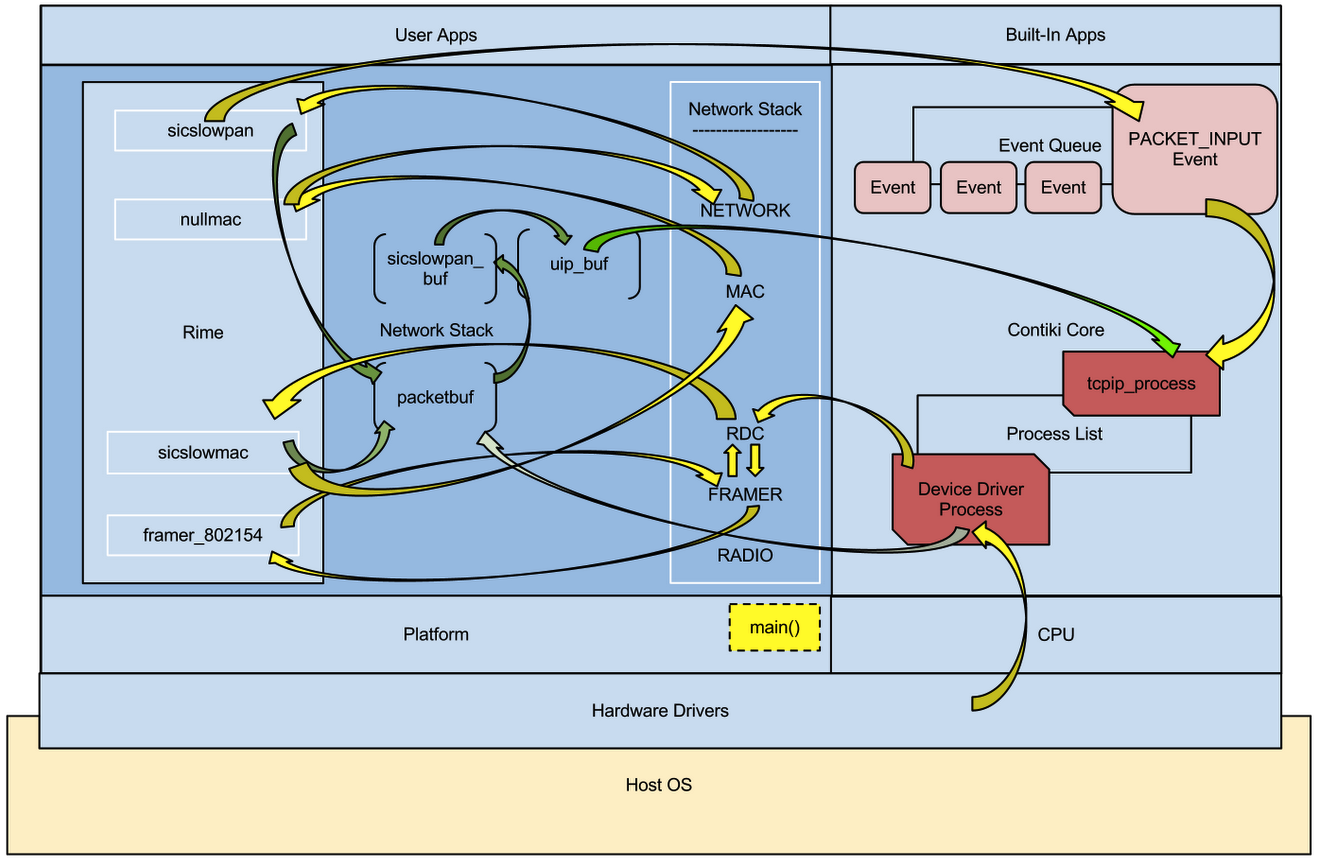
\includegraphics[width=12.5cm]{images/ch4-contiki-netstack.png}
\flcaption{Représentation fonctionnelle des dépendances au sein
de l'architecture de Contiki OS.
(Source~: \cite{BlogJUdit})}
\label{FigArchiReseauContiki}
\end{figure}

Cette complexité, combinée avec le manque de documentation (notamment
de références techniques), fait de toute tentative de contribution au code
de Contiki~--- et notamment de sa pile réseau~--- une tâche difficile,
pénible et sujette à de nombreuses erreurs.

\bigskip

En outre, comme ces difficultés sont des conséquences directes des principes
fondamentaux ayant présidé à la conception du système et de sa pile réseau,
il est difficilement envisageable de corriger ces défauts sans devoir
changer en profondeur l'architecture interne du système, ce qui
impliquerait bien évidemment des incompatibilités majeures (et donc
très probablement inacceptables pour la communauté des utilisateurs)
avec le code existant. Par conséquent, le besoin d'une documentation
technique précise, complète, détaillée et accessible est encore plus
critique.


\subsection{Fonctionnalités temps-réel insuffisantes}
\label{SubsecContikiTempsReel}

Pour implanter les protocoles avancés que nous avons décrit en section
\vref{SubsecProtoMACavances} du présent document, il est nécessaire de
gérer les évènements système (comme les interruptions) avec réactivité~---
c'est-à-dire avec un délai de latence minimal~--- et flexibilité. Ces
protocoles reposent en effet sur un \lang{timing} précis pour assurer
une synchronisation efficace entre les différents noeuds et autres
appareils appartenant aux différents réseaux de capteurs sans-fil (PANs),
permettant ainsi de faire fonctionner l'émetteur~/ récepteur radio des
noeuds seulement quand cela est nécessaire. L'émetteur~/ récepteur radio
est en effet le composant le plus gourmand en énergie dans ces noeuds,
et le mettre hors fonction est l'un des principaux moyens d'augmenter
la durée de vie de leur batterie.

Pour parvenir à une synchronisation temporelle suffisamment précise, nous
avons besoin d'une plate-forme logicielle offrant des fonctionnalités
temps-réel (c'est-à-dire garantissant que l'exécution d'une tâche donnée
se fera dans un délai respectant une échéance maximale donnée) avec une
granularité temporelle suffisamment fine.

Contiki, comme nous l'avons vu en section \vref{SubsecContikiOS}, n'est
pas à la base un système temps-réel~: le noyau est basé sur un ordonnanceur
évènementiel, basé sur du multitâche coopératif. Cet ordonnanceur ne se
déclenche qu'à intervalle fixe, pré-déterminé par une constante de
compilation. Sur les plates-formes que nous utilisons sous Contiki (les
\lang{motes} Sky/TelosB et Zolertia Z1), ce rythme de déclenchement de
l'ordonnanceur est fixé à 128~Hz, ce qui correspond à un délai de traitement
d'un évènement pouvant monter jusqu'à 8~millisecondes (8000~microsecondes),
sachant que le traitement d'une interruption fait partie des <<~évènements~>>
potentiels. Une granularité aussi large dans la réactivité du système est
clairement un problème majeur, notamment pour l'implantation de protocoles
MAC~/ RDC à hautes performances, sachant que la durée de transmission d'une
trame 802.15.4 de taille maximale (127 octets) est d'environ 4~millisecondes,
et que la durée de base d'une période de \lang{backoff} CSMA~/ CA est de
seulement 320~microsecondes.

Pour tenter de pallier ce problème, Contiki propose une fonctionnalité
dédiée à la gestion des évènements en temps-réel, nommée
\nom{\texttt{rtimer}}. Ce mécanisme permet d'outrepasser l'ordonnanceur
du noyau de Contiki, et d'utiliser un \lang{timer} matériel (c'est-à-dire
implanté comme périphérique physique dans le microcontrôleur au c{\oe}ur
du noeud) pour déclencher une fonction choisie par l'utilisateur.
Malheureusement, ce mécanisme souffre de sévères limitations~:

\begin{itemize}

\item Une seule et unique instance de \texttt{rtimer} est disponible pour
tout le système~; par conséquent, une seule tâche en temps-réel peut être
programmée ou exécutée à chaque instant. Cette limitation rend la
conception de programmes temps-réel un tant soit peu complexes~---
tel un protocole MAC~/ RDC, ou pire encore une pile réseau complète,
devant gérer simultanément plusieurs délais précis~--- plus difficile
à gérer et implémenter.

\item De plus, il est dangereux, pour la stabilité du système, d'exécuter
depuis une fonction déclenchée par \texttt{rtimer} la quasi-totalité
des fonctions de base de Contiki (c'est-à-dire~: le noyau, la pile réseau,
etc.), même de façon indirecte, car le code composant le c{\oe}ur de Contiki
n'a pas été conçu pour gérer la préemption (techniquement parlant, ces
fonctions ne sont pas <<~réentrantes~>>). Contiki est en effet basé sur
le paradigme du multitâche coopératif, tandis que \texttt{rtimer} se
comporte plutôt comme un mécanisme <<~indépendant~>>, venant avec son
propre paradigme. Seul un ensemble restreint de fonctions système définies
comme \lang{``interrupt-safe''} (par exemple~: la fonction
\texttt{process\_poll()}) peuvent être appelées en toute sécurité depuis
une <<~tâche~>> \texttt{rtimer}, l'utilisation de toute autre fonctionnalité
de Contiki conduisant de façon quasi-certaine à un plantage ou à un
comportement imprévisible du système. Cette restriction rend en pratique
le développement d'extensions temps-réel au système Contiki (via l'emploi
de \texttt{rtimer}) extrêmement difficile et limité.

\end{itemize}

Au final, et malgré l'introduction du mécanisme \texttt{rtimer}, qui est
comme nous venons de le voir extrêmement limité, il est impossible de
considérer Contiki comme un système temps-réel (même dans la définition
la plus <<~large~>> du terme).

\label{PtEchecSCosensContiki}
Une tentative d'implantation de S-CoSenS a malgré tout été réalisée
sous Contiki, mais pour les raisons citées dans la présente section
\ref{SecLimContiki}, il a été impossible de rendre celle-ci un tant soit
peu fonctionnelle. Suite à cet échec, nous avons donc définitivement
abandonné l'idée d'utiliser Contiki comme plate-forme logicielle pour
nos travaux de thèse, la présence de fonctionnalités temps-réel étant
indispensable pour pouvoir~:

\begin{itemize}

\item synchroniser de façon suffisamment précise les différents noeuds 
des WSN~;

\item ou même, ne serait-ce que pour respecter les durées des diverses
périodes et donc implanter de façon satisfaisante nos protocoles MAC~/ RDC
avancés.

\end{itemize}

%%%%%%%%%%%%%%%%%%%%%%%%%%%%%%%%%%%%%%%%%%%%%%%%%%%%%%%%%%%%%%%%%%%%%%%%%%%%%

\section{RIOT OS~: découverte et contributions}
\label{SecRIOTContrib}


\subsection{La plate-forme logicielle RIOT OS}
\label{SubSecPFRIOT}

Nous nous sommes alors intéressés à RIOT OS qui, comme indiqué dans
la section \vref{SubsecRIOTOS}, offre toutes les fonctionnalités dont
nous avons besoin pour nos développements, notamment~: un micro-noyau avec
un ordonnanceur fonctionnant selon le paradigme du multitâche préemptif,
ainsi que la possibilité d'utiliser les \lang{timers} matériels du
microcontrôleur, et ce avec une granularité au moins aussi fine
que le permettent ces \lang{timers} matériels.

Sur les premiers matériels que nous avons utilisés (TelosB et Z1), cette
granularité est d'environ $30,5~\mu$s (la fréquence des \lang{timers}
étant comme nous l'avons vu de 32~KHz). Une telle granularité est tout
à fait satisfaisante pour nos travaux.

RIOT OS a historiquement d'abord été développé~--- sous le nom de
<<~Feuerware~>>~--- sur des appareils à architecture ARM aujourd'hui
obsolètes (famille ARM7\-TDMI), puis a été porté sur des microcontrôleurs
plus récents (ARM Cortex-M) ainsi que d'autres architectures (MSP430
puis plus récemment Atmel AVR).

Toutefois, lorsque nous avons commencé à travailler avec RIOT (début 2014),
le portage sur MSP430 n'était pas aussi bien débogué que le code ARM, et
était souvent victime de plantages.


\subsection{Contributions au projet RIOT OS}
\label{SubSecContribRIOT}

Nos contributions, lors de cette première partie de nos travaux de thèse
sur RIOT OS, peuvent ainsi être résumées en les points suivants~:

\subsubsection{Gestion des erreurs fatales}
\label{ParRIOTCorePanic}

Nous avons d'abord \emph{ajouté des fonctionnalités de déboguage
au noyau de RIOT OS, et notamment un mécanisme destiné à prendre en charge
les erreurs fatales} \cite{PRriotPanic}.

\smallskip

Cet ajout s'est inspiré de la fonction noyau \texttt{panic()} bien
connue dans le monde des systèmes Unix et dérivés. Cette fonction,
en générale interne au noyau système, sert à gérer les erreurs fatales,
en arrêtant le système, en essayant souvent de fournir le maximum
d'informations concernant le problème survenu, et si possible en
limitant les risques de dommages (notamment aux données stockées
sur le système, voire dans certains rares cas au matériel).
Cette procédure d'arrêt <<~en catastrophe~>> du système est nommée,
dans le monde <<~unixien~>>, \emph{``kernel panic''}.

Son équivalent dans les systèmes Microsoft (Windows) et autres
(OS/2, iOS) est le \lang{``Screen of Death''}~--- le plus souvent bleu
ou noir (d'où l'acronyme BSOD).

Dans ces systèmes destinés à l'informatique <<~lourde~>> (des PC
aux macro-ordinateurs), \texttt{panic()} est une fonction interne
au noyau, car ce dernier s'appuie sur des dispositifs matériels de
gestion de la mémoire (à savoir une \nom{MMU}~: unité de gestion
de mémoire), rendant la majorité des programmes~--- nommément
tous ceux ne s'exécutant pas en <<~mode privilégié~>> ou <<~espace
mémoire noyau~>>, c'est-à-dire normalement toutes les applications
lancées par l'utilisateur~--- incapables d'endommager les structures
de données et autres ressources vitales pour l'exécution du système.
Ces programmes ne manipulent en effet, via le fonctionnement d'une MMU
en mode <<~non privilégié~>> ou <<~utilisateur~>>, que des adresses
<<~logiques~>> (également parfois appelées adresses <<~linéaires~>> ou
<<~virtuelles~>>) au sein d'un espace mémoire virtuel propre à chaque
programme en cours d'exécution~; la manipulation réelle des adresses
physiques sous-jacentes se faisant exclusivement au travers de la MMU et
de ses stricts mécanismes de sécurité et de séparation des espaces mémoires,
configurés par le noyau. Un programme en <<~mode utilisateur~>> est ainsi
normalement incapable de corrompre tout espace mémoire différent du sien,
que ce soit celui des autres applications, ou \lang{a fortiori} celui du
c{\oe}ur du système.
Une erreur fatale ne peut par conséquent normalement survenir que lorsqu'un
problème survient dans le code s'exécutant en <<~mode privilégié~>>
(c-à-d~: code du noyau lui-même, ou pilotes de périphériques).

\smallskip

Dans les systèmes embarqués, il n'y a pas de MMU~: tout au plus
une \nom{MPU} (unité de protection mémoire) offrant une limitation d'accès
à certaines zones mémoire selon le mode (privilégié ou non).

Malheureusement, toutes les architectures de processeurs embarqués
n'offrent pas ce mécanisme de MPU~: il n'existe pas dans les
architectures AVR et MSP430, et n'est qu'optionnel pour les ARM
(notamment Cortex-M), beaucoup de microcontrôleurs implantant cette
dernière architecture font ainsi l'impasse sur ce mécanisme.

Il faut également préciser que les applications (souvent uniques) d'un
système embarqué ayant régulièrement besoin d'accéder directement aux
ressources matérielles~--- notamment pour des raisons d'efficacité~---
beaucoup d'entre elles sont, pour des raisons de simplicité, programmées
pour fonctionner exclusivement en mode privilégié, rendant ainsi tout
mécanisme de MPU inopérant.

Pour toutes ces raisons RIOT OS (du moins dans les versions \texttt{2013.08}
à \texttt{2015.12} incluses, que nous avons utilisées dans le cadre de
la présente thèse) n'utilise aucune MPU, même sur les architectures
où un tel mécanisme est présent.

\smallskip

Ainsi, nous avons dès le départ clairement déterminé qu'une fonction
de gestion des erreurs fatales ne saurait être un mécanisme interne
au noyau de RIOT, mais devrait être une primitive système explicitement
offerte par ce dernier à l'ensemble du code~--- noyau, pilotes et
applications système. Cette fonction a été, après discussion avec le
reste de l'équipe de développement, nommée \nom{\texttt{core\_panic()}}.

Nous avons voulu reproduire le maximum des possibilités offertes
par les procédures équivalentes des systèmes pour l'informatique
<<~classique~>> (PC et autres)~: les systèmes <<~plantés~>> peuvent
ainsi être <<~gelés~>> pour faciliter leur déboguage durant les phases de
développement~; ou, en production, être au contraire immédiatement
redémarrés, réduisant ainsi l'indisponibilité d'un appareil fonctionnant
sous RIOT au minimum~; le choix entre les deux comportements se fait
via une constante de compilation.

Cette contribution s'est vue décerner le titre de \emph{``PR of the
month''} pour le mois de février 2014 par le projet RIOT OS.

Cette contribution utilise une autre de nos contributions implantant
une primitive de redémarrage (fonction \texttt{reboot()}) au noyau de RIOT
pour le mode production \cite{PRriotEnh5} \cite{PRriotEnh3}.

\subsubsection{Portage sur une nouvelle plate-forme matérielle}
\label{ParRIOTZolertiaZ1}

Nous avons \emph{porté RIOT OS sur la Zolertia Z1} \cite{PRriotPortZ1},
qui est rappelons-le une \lang{mote} basée sur l'architecture MSP430,
utilisée de façon industrielle (notamment avec Contiki).

\smallskip

Dans la plupart des systèmes d'exploitation visant la portabilité (comme
par exemple Unix~/ Linux, ou les différentes déclinaisons de Microsoft
Windows NT), la majorité du code du système est conçue de façon générique,
c'est-à-dire avec une structure et un fonctionnement indépendants de la
plate-forme matérielle sous-jacente.

Le code dépendant de la plate-forme est réduit au minimum, et se charge
d'offrir au reste (très majoritaire) du système une API prédéfinie
lui permettant d'accéder au matériel tout en <<~ignorant~>> ces
spécificités. L'ensemble restreint de ce code dépendant des plates-formes
matérielles et cachant les disparités de ces dernières est nommé
\nom{couche d'abstraction matérielle} (\nom{HAL~:} \lang{Hardware
Abstraction Layer}).

\smallskip

RIOT OS, comme la plupart des systèmes portables, est conçu selon ce modèle
employant une couche d'abstraction matérielle. Un portage de RIOT OS sur un
nouveau matériel consiste donc à créer une variante de cette couche capable
de gérer la nouvelle plate-forme matérielle visée.

Cette couche d'abstraction matérielle se charge notamment, sous RIOT OS,
d'assurer le support des changements de contexte lors des basculements entre
tâches (en support à l'ordonnanceur), l'implantation des fonctions concernant
les \lang{timers} ou les différents périphériques implantés au sein du
microcontrôleur, ainsi que l'accès aux entrées~/ sorties (GPIO). Du point
de vue de l'implantation, la couche d'abstraction matérielle peut être vue
comme un ensemble de pilotes (\lang{``drivers''}) chargés d'implanter l'API
prédéfinie entre cette couche et le reste du système d'exploitation~;
ces pilotes doivent en général lire et écrire les registres matériels
de façon adéquate, en fonction des opérations demandées.

\smallskip

La couche d'abstraction matérielle de RIOT OS se divise fonctionnellement
en plusieurs sous-parties~:

\begin{enumerate}

\item Une partie <<~\emph{MCU}~>> destinée à supporter les différentes
architectures de microcontrôleurs visées. Cette partie prend en charge les
fonctionnalités spécifiques de chaque architecture de microcontrôleur,
elle regroupe ainsi le code commun entre plates-formes matérielles basées sur
des microcontrôleurs similaires (ARM7, Cortex-M, MSP430, AVR...). Dans notre
cas, le code commun destiné à supporter l'architecture MSP430 existait déjà~:
nous n'avons ainsi pas eu à nous occuper de cette partie MCU pour effectuer
notre portage.

Cette partie de la couche d'abstraction matérielle se charge notamment des
opérations liées aux registres et mécanismes du c{\oe}ur du microcontrôleur~:
par exemple de l'implantation des changements de contexte lors des
basculements entre tâches.

\item Une partie <<~\emph{périphériques}~>> regroupant des pilotes génériques
pour des circuits intégrés communs, susceptibles d'être retrouvés dans
plusieurs matériels différents~: c'est le cas des émetteurs~/ récepteurs
radio, des capteurs environnementaux divers (ex.~: température, humidité,
etc.). Nous n'avons pas non plus eu besoin pour ce travail de portage
d'intervenir directement sur cette partie.

Ces pilotes <<~génériques~>> sont ensuite exploités de façon adéquate par
du code <<~de liaison~>> (\lang{``glue''} en anglais) spécifique~---
impliquant souvent un bus géré par le microcontrôleur comme SPI ou
I\textsuperscript{2}C~--- permettant leur mise en {\oe}uvre sur chaque
plate-forme matérielle différente. Ce code de liaison est implanté dans
la dernière partie de la couche d'abstraction matérielle décrite ci-dessous.

\item Une partie <<~\emph{plate-forme}~>> regroupant les éléments
véritablement spécifiques à une plate-forme matérielle donnée. Elle
regroupe notamment les pilotes du matériel purement spécifique à une
plate-forme donnée, ainsi que le code <<~de liaison~>> (\lang{``glue''})
avec les parties plus génériques de la couche d'abstraction matérielle.
C'est cette partie que nous avons créée pour le support spécifique de
la plate-forme matérielle Zolertia Z1.

Ce travail, comme nous l'avons dit ci-dessus, a principalement consisté
à implanter des pilotes~--- notamment pour les \lang{timers} matériels,
le port série~/ USB (UART) et les GPIO~--- ainsi qu'une fonction
d'initialisation adéquate, principalement en manipulant les registres
adéquats des périphériques. Nous avons également créé le code de liaison
nécessaire avec le pilote pré-existant pour l'émetteur~/ récepteur radio
CC2420 qui équipe cette \lang{mote}, via la configuration adéquate du bus
SPI du microcontrôleur.

\end{enumerate}

\subsubsection{Déboguage des portages sur MSP430}
\label{ParRIOTDebugMSP430}

Nous avons \emph{débogué les portages de RIOT OS sur MSP430}~--- plus
précisément~: la portion spécifique de la couche d'abstraction matérielle
de l'ordonnanceur chargée de traiter les changements de contexte
lors des basculements entre tâches \cite{PRriotFix2MSP430}
\cite{PRriotFix3MSP430} \cite{PRriotFix1MSP430}~--- rendant ainsi RIOT
robuste et prêt à l'usage en production sur les appareils basés sur
l'architecture MSP430.

\smallskip

Pour effectuer un tel déboguage de façon efficace, il est nécessaire~:

\begin{itemize} 

\item Soit de disposer de la possibilité de faire appel à des fonctions
de déboguage directement présentes dans le matériel, en général rendues
accessibles via le protocole JTAG. La plupart des microcontrôleurs
sur lesquels sont basées les \lang{motes} offrent des broches spécifiques
dédiées à ce mécanisme de déboguage~; il faut néanmoins que la \lang{mote}
elle-même rende ces signaux accessibles via un port quelconque, ce qui
n'est pas évident. En outre, un adaptateur JTAG, presque toujours spécifique
de l'architecture du microcontrôleur à déboguer, est nécessaire pour relier
le matériel à déboguer et le PC~/ station de travail du développeur.
Enfin, le protocole JTAG ne permet sauf exception que d'agir sur le
microcontrôleur lui-même, pas d'avoir accès aux circuits annexes comme
les émetteurs~/ récepteurs radio autonomes (tel le CC2420 de la Zolertia
Z1).

\item Soit de disposer d'un émulateur suffisamment fiable, et fidèle au
fonctionnement réel du matériel sur lequel le programme à déboguer doit
s'exécuter. Celui-ci peut alors offrir des fonctions de déboguage avancées,
comparables à ce qu'offrent les environnement de développement pour PC.
Un tel émulateur est MSPSim \cite{MSPSim}, fourni en standard avec le
simulateur de réseaux de capteurs sans-fil Cooja \cite{Cooja} du projet
Contiki, lequel émule plusieurs \lang{motes} basées sur l'architecture
MSP430, notamment les TelosB~/SkyMotes et~--- surtout~--- la Zolertia Z1.

\end{itemize}

\smallskip

Les problèmes qui touchaient les portages de RIOT OS sur MSP430 étaient mal
reproductibles, car imprévisibles (bien que fréquents)~: leur déclenchement
n'ayant pu être lié ni à l'utilisation d'une certaine fonctionnalité, ni au
passage dans une portion spécifique du code de RIOT, ni à l'écoulement d'un
certain délai. Dans ces conditions, il est très difficile de trouver la
cause d'un problème, même en utilisant les meilleurs outils de déboguage.

Pour trouver la raison principale des plantages de RIOT OS sur MSP430,
nous avons eu recours à la technique dite de \nom{traçage des instructions~:}
cette technique consiste à enregistrer chaque instruction exécutée par
le matériel lors du fonctionnement du code défectueux (soit pour toute
la durée d'exécution, soit pour un intervalle de temps donné). Au final,
l'utilisation de cette technique permet d'obtenir un \lang{listing}
assembleur précis, reproduisant fidèlement les instructions élémentaires
exécutées lors du déroulement du programme.

Employer la technique de traçage avec un débogueur matériel nécessite
l'emploi d'un adaptateur JTAG haut de gamme, disposant de la quantité
de mémoire nécessaire pour enregistrer les instructions exécutées. De tels
adaptateurs sont coûteux, et n'existent pas pour toutes les architectures~:
l'unique adaptateur JTAG MSP430 vendu par Texas Instruments ne dispose pas
d'une telle fonctionnalité.

À l'inverse, \emph{le couple Cooja~/ MSPSim offre une telle fonctionnalité
de traçage des instructions}. Nous avons donc utilisé cette possibilité,
qui nous a finalement permis de découvrir la source de la principale cause
d'instabilité sur MSP430, à savoir~: l'inactivation trop tardive des
interruptions pendant le changement de contexte de tâche, permettant
à une interruption de stopper la sauvegarde du contexte de la tâche
en cours d'arrêt, ce qui bien évidemment corrompait le plus souvent
le contexte sauvegardé, provoquant le plantage du système lors de la
réactivation de la tâche touchée. Cette réactivation intervenant de façon
non déterministe, en fonction de la charge du système et de sa gestion par
l'ordonnanceur, on comprend ainsi pourquoi ces plantages intervenaient
sans raison \lang{a priori} discernable. Nous avons donc, grâce aux
fonctions avancées de déboguage et traçage de MSPSim, pu comprendre
le principal problème et y apporter une solution. Cette solution consiste
à corriger l'ordre des instructions dans la fonction \texttt{thread\_yield()},
faisant partie de la partie de la couche d'abstraction matérielle de RIOT
gérant l'architecture MSP430~: les interruptions sont désormais désactivées
dès le début de la fonction, \emph{avant} de commencer à sauvegarder le
contexte du \lang{thread} en cours de suspension, et ne sont réactivées
(si nécessaire) qu'une fois le contexte du \lang{thread} à relancer
totalement restauré \cite{PRriotFix2MSP430}.

La correction de deux autres problèmes liés à la gestion des \lang{timers}
des MSP430 par cette même couche d'abstraction matérielle, plus simples à
comprendre et à résoudre, a permis d'achever la fiabilisation des portages
de RIOT OS~:
\begin{enumerate}
\item la correction de l'implantation de la fonction \texttt{hwtimer\_spin()},
en évitant que ne soit calculée une valeur-cible impossible à atteindre
par le compteur du \lang{timer} voulu \cite{PRriotFix1MSP430}~;
\item l'abandon de la prise en charge de délais supérieurs à $2^{16}$
\lang{``ticks''} de \lang{timers} pour l'implantation du mécanisme
\texttt{hwtimer} sur MSP430 \cite{PRriotFix3MSP430}.
\end{enumerate}
Ces deux erreurs étaient dues à la différence de type entre les valeurs
calculées par les implantations des fonctionnalités liées aux mécanismes
temps-réel de \texttt{hwtimer}~--- utilisant des entiers~32 bits~--- et
les compteurs des \lang{timers} matériels des MSP430~--- qui ne sont
que des entiers de 16~bits \footnotemark[2].

\footnotetext[2]{Ce type de problèmes et limitations a conduit au
remplacement du mécanisme \texttt{hwtimer} par le module \texttt{xtimer},
de conception différente et de plus haut niveau (comme vu en section
\vref{SubsecRIOTOS}), et donc normalement moins vulnérable vis-à-vis
de telles difficultés d'implantation.}

\medskip

La possibilité de faire fonctionner RIOT sur MSP430 permet donc
\emph{d'exécuter des applications basées sur ce système dans le simulateur
Cooja~/ MSPSim. Cela facilite grandement la rapidité et l'efficacité
du développement de telles applications.} Nous venons notamment de le
démontrer, le déboguage de la couche d'abstraction matérielle de RIOT pour
les microcontrôleurs MSP430 aurait probablement été extrêmement difficile
sans ses fonctionnalités de déboguage et notamment de traçage.

Au final, on voit qu'un émulateur \emph{de qualité} peut se révèler un outil
de développement et déboguage extrêmement précieux, en complément des
débogueurs matériels, ou même en remplacement de ces derniers, lorsque
ceux-ci sont trop coûteux ou~--- surtout~!~--- n'offrent pas les
fonctionnalités nécessaires comme cela a été le cas ici. Bien évidemment,
\emph{l'émulateur en question, pour remplir ce rôle, doit être très fidèle
au fonctionnement du matériel émulé pour être utile}. Dans ce cas précis,
MSPSim s'est révélé tout à fait à la hauteur quant à l'émulation du c{\oe}ur
du microcontrôleur MSP430 (au niveau duquel se produisait le bogue à
corriger).

\subsubsection{Contributions diverses}
\label{ParRIOTContribDiverses}

D'autres contributions ont été apportées, ayant eu un impact moindre sur
l'avancée du projet RIOT OS. Celles-ci se divisent en deux groupes~:

\begin{enumerate}

\item les contributions de \emph{déboguage}~:
\begin{itemize}
\item réparation du mécanisme d'échange de données entre microcontrôleur et
émetteur~/ récepteur radio sur Zolertia Z1, en corrigeant le test vérifiant
la bonne émission d'un octet sur le bus SPI (retrait d'une négation logique
erronée) \cite{PRriotDebug9},
\item correction de diverses erreurs dans le pilote pour l'émetteur~/
récepteur radio CC2420 au niveau de l'implantation~: correction d'une
constante \cite{PRriotDebug3}, de la gestion des adresses et du PAN ID
\cite{PRriotDebug2}, de la gestion du bus SPI pour communiquer avec
la radio (notamment la fonction \texttt{cc2420\_do\_send()})
\cite{PRriotDebug7}, et dans la détermination du CCA (mauvaise gestion
du bus SPI dans l'implantation de cette fonctionnalité) \cite{PRriotDebug8},
\item correction d'erreurs intermittentes concernant les \lang{timers}
matériels des MCU MSP430, notamment en déclarant certaines variables
\texttt{volatile}s au sein de l'implantation \cite{PRriotDebug4},
\item fiabilisation des mécanismes de gestion des interruptions sur
architecture MSP430, en ajoutant un <<~délai d'attente~>> (instruction
\texttt{NOP}) après l'activation ou la désactivation générale des
interruptions au niveau du microcontrôleur (comme recommandé dans les
manuels de TI), et en s'assurant que les interruptions sont bien activées
avant l'entrée en mode basse consommation (pour pouvoir sortir de ce
dernier) \cite{PRriotDebug10},
\item fiabilisation de l'alignement du pointeur de pile (registre SR)
lors de la création de threads \cite{PRriotDebug1},
\item fiabilisation du processus de \lang{flashage} des applications sur
ARM Cortex-M3, en forçant un effacement de la mémoire et un \lang{reset}
avant le lancement du processus de \lang{flashage} proprement dit
\cite{PRriotDebug6},
\item correction et la fiabilisation de la fonction d'attente active via
l'utilisation des timers matériels (\texttt{hwtimer\_spin()}), en modifiant
l'implantation pour la rendre plus simple, compréhensible et fiable
\cite{PRriotDebug5}~;
\end{itemize}

\item les contributions \emph{apportant des améliorations et fonctionnalités
supplémentaires}~:
\begin{itemize}
\item amélioration de l'API et des fonctionnalités des pilotes des
émetteurs~/ récepteurs radio \cite{PRriotEnh12} \cite{PRriotEnh10}
\cite{PRriotEnh11} \cite{PRriotEnh7} \cite{PRriotEnh6},
\item gestion des modes <<~basse énergie~>> des MCU MSP430
\cite{PRriotEnh2},
\item réorganisation et simplification des fichiers d'entête
(\texttt{xxx.h}) pour la partie MSP430 de la couche d'abstraction
matérielle \cite{PRriotEnh1},
\item augmentation du nombre d'instances de \lang{timers} matériels
(\texttt{hwtimer}s) utilisables sur MSP430 \cite{PRriotEnh9},
\item ajout d'une primitive de redémarrage (fonction \texttt{reboot()})
au noyau de RIOT (notamment employée par la gestion des erreurs fatales
pour réactiver au plus vite un système planté en mode production, voir
\vref{ParRIOTCorePanic}) \cite{PRriotEnh5} \cite{PRriotEnh3},
\item définition d'attributs de fonction <<~portables~>> \cite{PRriotEnh4},
\item possibilité pour un thread d'envoyer un message à lui-même
(pour permettre par exemple les appels de fonction retardés~---
\lang{``deferred procedure calls''} en anglais) \cite{PRriotEnh8},
\item ajout d'une option pour la gestion du \lang{``CCA threshold''}
dans la nouvelle pile gnrc \cite{PRriotEnh13}.
\end{itemize}

\end{enumerate}

\medskip

Notons que toutes ces contributions ont été revues et acceptées par
l'équipe de développement de RIOT, qui les a intégrées dans le source
\lang{``master''} du système~: elles font donc maintenant partie du
système de base \footnotemark[3].

\footnotetext[3]{Les changements récents dans la pile réseau et la gestion
des \lang{timers} du système RIOT ont toutefois rendu obsolète le code
apporté par certaines de ces contributions~; néanmoins, les fonctionnalités
correspondantes ont en général été réimplantées d'une façon différente
et adéquate dans les nouvelles versions de RIOT OS.}

\bigskip

Grâce à toutes ces avancées, nous avons maintenant une plate-forme
logicielle robuste et offrant les fonctionnalités nécessaires pour
développer nos protocoles MAC~/ RDC à hautes performances~--- notamment
ceux basés sur l'ordonnancement temporel (TDMA).
C'est pourquoi nous avons implanté et testé S-CoSenS sur RIOT OS lors des
expériences que nous décrirons au chapitre \vref{ChProtocolesMAC}.


\subsection{\'Evolution du système RIOT OS}
\label{SubSecEvoRIOT}

Depuis que lesdites expériences du chapitre \ref{ChProtocolesMAC} ont
été menées, RIOT OS a continué à évoluer de façon rapide et profonde~---
et tout particulièrement sa pile réseau, qui a fait l'objet d'une refonte
totale. Cette évolution étant potentiellement amenée à modifier, non
seulement les résultats des expériences citées ci-dessus, mais aussi
ceux des travaux présentés plus loin au chapitre \vref{ChValidation}
(et notamment à influer sur les problèmes détaillés dans ce dernier
chapitre), nous allons maintenant procéder à une analyse détaillée
et critique de cette nouvelle pile réseau.

%%%%%%%%%%%%%%%%%%%%%%%%%%%%%%%%%%%%%%%%%%%%%%%%%%%%%%%%%%%%%%%%%%%%%%%%%%%%%

\section{La nouvelle pile réseau de RIOT~: une analyse critique}
\label{SecGnrcRIOT}

Nous décrivons, dans les sections \vref{ParAPIRadioContiki} puis
\vref{SubsecAPIRadioExt}, notre mécanisme de <<~capacités~>> permettant
de profiter de façon portable des spécificités des émetteurs~/ récepteurs
radio des \lang{``motes''}, grâce à des fonctions génériques de gestion
d'un ensemble varié et extensible de constantes et paramètres.
Un mécanisme de ce type est désormais intégré dans Contiki 3.0
\cite{Contiki3Annonce} (suite en partie et de façon indirecte à certaines
de nos contributions). Une évolution similaire a eu lieu pour RIOT OS.

En effet, pendant que nous tentions d'effectuer nos travaux
et subissions les problèmes techniques détaillés dans la section
\vref{SecTravauxMiseOeuvre}, RIOT OS a durant l'année 2015 subi une
refonte de sa pile réseau~--- une pile réseau nouvelle génération,
se voulant générique (\nom{<<~gnrc~>>}), est apparue, sur laquelle
nous allons nous pencher dans la présente section.

Compte-tenu du sujet de la présente thèse, nous nous focaliserons sur les
couches les plus basses (physique~/ pilote radio, et MAC~/ RDC) de cette
nouvelle pile.


\subsection{Description}
\label{SubsecDescrGnrc}

L'API des pilotes pour les émetteurs~/ récepteurs radio de la nouvelle
pile <<~gnrc~>> a repris le principe de ce que nous avons appelé le
mécanisme de <<~capacités~>>, implantant pour les pilotes radio
un ensemble, extrêmement réduit, de fonctions génériques, dont le
détail est donné en table \vref{TblGnrcFnct}. (Notons toutefois que nous
n'avons pas pu participer à l'implantation de ces nouveaux pilotes,
ni à la conception de la nouvelle pile <<~gnrc~>>, étant monopolisés
par nos propres travaux.)


\begin{table}[!hbt]
\centering

\begin{tabular}{|l|p{9cm}|}
\hline
\textbf{Nom} & \textbf{Rôle} \\
\hline
\texttt{send\_data()} & Envoie une trame via l'émetteur~/ récepteur radio \\
\hline
\texttt{add\_event\_callback()} & Ajoute une fonction \lang{``callback''}
                                  pour la gestion des évènements remontés
                                  par le pilote radio donné \\
\hline
\texttt{rem\_event\_callback()} & Retire une fonction \lang{``callback''}
                                  pour la gestion des évènements remontés
                                  par le pilote radio donné \\
\hline
\texttt{get()} & Lit la valeur courante d'une option de configuration
                 d'un pilote radio donné \\
\hline
\texttt{set()} & Définit la valeur courante d'une option de configuration
                 d'un pilote radio donné \\
\hline
\texttt{isr\_event()} & Fonction \lang{``callback''} pouvant être
                        appelée par une couche supérieure de la pile
                        réseau, pour signaler un évènement au pilote
                        radio (cet <<~évènement~>> étant actuellement
                        une valeur numérique totalement arbitraire) \\
\hline
\end{tabular}

\flcaption{Liste des fonctions des pilotes radio nouvelle génération
(<<~gnrc~>>).}
\label{TblGnrcFnct}
\end{table}


Les <<~évènements~>> pour lesquels il est possible de définir des
\lang{``callbacks''} sont listés en table \vref{TblGnrcEvnt}.
(Le déclenchement ou non de ces \lang{``callbacks''} se fait en fonction
de la valeur des options \texttt{NETOPT\_*\_*\_IRQ} définies en table
\vref{TblGnrcCapabOpt}.)


\begin{table}[!htb]
\centering

\begin{tabular}{|l|p{8cm}|}
\hline
\textbf{Nom} & \textbf{Signification} \\
\hline
\texttt{NETDEV\_EVENT\_RX\_STARTED} & Début de réception d'une trame (SFD) \\
\hline
\texttt{NETDEV\_EVENT\_RX\_COMPLETE} & Réception d'une trame terminée~:
                                       analyse possible du contenu \\
\hline
\texttt{NETDEV\_EVENT\_TX\_STARTED} & Début de transmission d'une trame \\
\hline
\texttt{NETDEV\_EVENT\_TX\_COMPLETE} & Fin de transmission d'une trame \\
\hline
\end{tabular}

\flcaption{Liste des évènements radio interceptables (<<~gnrc~>>).}
\label{TblGnrcEvnt}
\end{table}


Les différentes options pouvant être réglées par les fonctions \texttt{get()}
et \texttt{set()} sont listées dans la table \vref{TblGnrcCapabOpt}.


\begin{table}[!p]
\centering

\small
\begin{tabular}{|l|p{9cm}|}
\hline
\textbf{Identifiant} & \textbf{Signification} \\
\hline
\texttt{NETOPT\_CHANNEL} & Canal (fréquence) utilisée
                          par l'émetteur~/ récepteur radio \\
\hline
\texttt{NETOPT\_IS\_CHANNEL\_CLR} & Vérifie si le médium radio est disponible
                                 (\lang{``Clear Channel Assessment''}) \\
\hline
\texttt{NETOPT\_ADDRESS} & Définit l'adresse <<~courte~>> (intra-PAN,
                          16 bits) de la radio \\
\hline
\texttt{NETOPT\_ADDRESS\_LONG} & Définit l'adresse <<~longue~>> (64 bits pour
                               le 802.15.4) de la radio \\
\hline
\texttt{NETOPT\_ADDR\_LEN} & Taille de l'adresse longue de la radio
                           (normalement 64 bits pour le 802.15.4) \\
\hline
\texttt{NETOPT\_SRC\_LEN} & Taille de l'adresse source à utiliser
                          pour la radio \\
\hline
\texttt{NETOPT\_NID} & Définit l'identifiant du réseau (PAN ID) \\
\hline
\texttt{NETOPT\_IPV6\_IID} & Définit l'adresse IPv6 de l'interface réseau
                           (RFC 4291, section 2.5.1) \\
\hline
\texttt{NETOPT\_TX\_POWER} & Définit la puissance d'émission
                           de la radio en dBm \\
\hline
\texttt{NETOPT\_MAX\_PACKET\_SIZE} & Définit la taille maximale d'une trame
                                  (normalement 127 octets pour le 802.15.4) \\
\hline
\texttt{NETOPT\_PRELOADING} & Active ou désactive la possibilité de
                             pré-charger le \lang{``buffer''} de
                             transmission de la radio sans lancer
                             immédiatement l'émission de la trame \\
\hline
\texttt{NETOPT\_PROMISCUOUSMODE} & Active ou désactive le mode <<~moniteur~>>
                                  (\lang{``promiscuous''}) \\
\hline
\texttt{NETOPT\_AUTOACK} & Active ou désactive l'acquittement automatique
                          des trames reçues par la radio \\
\hline
\texttt{NETOPT\_RETRANS} & Nombre maximal de retransmissions en mode CSMA/CA \\
\hline
\texttt{NETOPT\_PROTO} & Type de protocole (6LoWPAN, IPv6, TCP, UDP...)
                        pour la couche voulue \\
\hline
\texttt{NETOPT\_STATE} & \'Etat de la radio, à choisir parmi~:
                        \begin{itemize}
                        \item \texttt{NETOPT\_STATE\_OFF}~: hors tension
                        \item \texttt{NETOPT\_STATE\_SLEEP}~: mode inactif
                              basse consommation
                        \item \texttt{NETOPT\_STATE\_IDLE}~: en écoute
                              (passive)
                        \item \texttt{NETOPT\_STATE\_RX}~: réception en cours
                        \item \texttt{NETOPT\_STATE\_TX}~: transmission en
                              cours / déclenche l'émission d'une trame
                              préchargée
                        \item \texttt{NETOPT\_STATE\_RESET}~: provoque
                              une réinitialisation de la puce radio
                        \end{itemize} \\
\hline
\texttt{NETOPT\_RAWMODE} & Active ou désactive l'analyse automatique des
                          trames reçues \\
\hline
\texttt{NETOPT\_RX\_START\_IRQ} & Active ou désactive le déclenchement d'une
                               interruption au début d'une réception (SFD) \\
\hline
\texttt{NETOPT\_RX\_END\_IRQ} & Active ou désactive le déclenchement d'une
                             interruption lors de la réception d'une trame
                             complète \\
\hline
\texttt{NETOPT\_TX\_START\_IRQ} & Active ou désactive le déclenchement d'une
                               interruption au début d'une transmission \\
\hline
\texttt{NETOPT\_TX\_END\_IRQ} & Active ou désactive le déclenchement d'une
                             interruption à la fin de la transmission
                             d'une trame \\
\hline
\texttt{NETOPT\_AUTOCCA} & Active ou désactive la vérification automatique
                          de la disponibilité du médium radio
                          (\lang{``Clear Channel Assessment''})
                          par l'émetteur~/récepteur radio au début
                          d'une transmission \\
\hline
\end{tabular}

\flcaption{\small Liste des options~--- <<~capacités~>> potentielles~---
des émetteurs~/ récepteurs radio (<<~gnrc~>>).}
\label{TblGnrcCapabOpt}
\end{table}


Les fonctions présentées en table \vref{TblGnrcFnct} signalent
la survenue d'erreurs en retournant les valeurs d'erreurs (toujours
négatives) listées en table \vref{TblGnrcErr}.


\begin{table}[htb]
\centering

\begin{tabular}{|l|p{10cm}|}
\hline
\textbf{Nom} & \textbf{Signification} \\
\hline
\texttt{-ENODEV}    & Tentative d'accès à un pilote radio
                      \texttt{gnrc\_netdev\_t} invalide
                      (toutes les fonctions) \\
\hline
\texttt{-ENOMSG}    & Tentative d'envoi d'une trame invalide
                      (fonction \texttt{send\_data()}) \\
\hline
\texttt{-EOVERFLOW} & Le \lang{buffer} chargé de contenir la trame à
                      envoyer, ou les données du paramètre à lire est
                      trop petit (fonctions \texttt{send\_data()}
                      et \texttt{get()})\\
\hline
\texttt{-ENOBUFS}   & Le nombre maximal de fonctions \lang{``callbacks''}
                      pour un pilote radio donné est dépassé
                      (fonction \texttt{add\_event\_callback()}) \\
\hline
\texttt{-ENOENT}    & La fonction \lang{``callback''} à retirer n'a pas
                      été enregistrée auparavant
                      (fonction \texttt{rem\_event\_callback()})\\
\hline
\texttt{-ENOTSUP}   & Option non supportée par ce pilote radio
                      (fonctions \texttt{get()} et \texttt{set()}) \\
\hline
\texttt{-ECANCELED} & Erreur interne du pilote radio
                      (fonctions \texttt{get()} et \texttt{set()}) \\
\hline
\texttt{-EINVAL}    & Valeur invalide pour l'option transmise
                      (fonction \texttt{set()}) \\
\hline
\end{tabular}

\flcaption{Liste des erreurs potentiellement renvoyées (<<~gnrc~>>).}
\label{TblGnrcErr}
\end{table}


(Notons que les tables \vrefrange{TblGnrcFnct}{TblGnrcErr} représentent
l'état d'avancement de la pile <<~gnrc~>> au moment où nous écrivons
ces lignes~--- début septembre 2015. Cette pile étant toujours  à l'heure
actuelle l'objet d'un développement rapide et poussé, le contenu de ces
tables ne sera sans doute plus exhaustif au moment où ce manuscrit
de thèse sera lu.)

\bigskip

Le pilote radio amélioré, implantant notre concept de <<~capacités~>>,
dont nous discuterons en section \vref{SubsecAPIRadioExt} est donc déjà
obsolète, et ne sera pas intégré au code de RIOT OS.

En effet, un nouveau type de pilote radio, nommé \texttt{gnrc\_netdev\_t},
a été créé~; toutes les fonctions de la nouvelle API <<~gnrc~>> travaillent
avec des instances de ce type.

Un effort pour convertir tous les pilotes radio de RIOT à l'API de ce
nouveau type \texttt{gnrc\_netdev\_t} est actuellement en cours.


\subsection{Avantages}
\label{SubsecAvantagesGnrc}

On peut voir ici que le travail de refonte de la pile a été poussé très
loin, et que le jeu d'options réglables grâce à la nouvelle API est déjà
très complet. La logique de la gestion générique des paramètres est poussée
jusqu'au bout~: seul l'envoi de trames et la réception d'évènements~---
ce qui inclut la réception de trames~--- coexistent encore avec la paire
de fonctions \texttt{get()} et \texttt{set()} gérant les paramètres.

Nous avons avec ces nouveaux pilotes radio d'ores et déjà le mécanisme
nécessaire pour compter les SFDs, que nous comptions utiliser pour améliorer
S-CoSenS. La seule option que nous pourrions vouloir ajouter serait celle
permettant de définir le seuil de distinction signal~/ bruit (\lang{``CCA
Threshold''}), par exemple via une option \texttt{NETOPT\_CCA\_THRESHOLD}.
Un tel ajout sera probablement très facile à réaliser dans cette nouvelle
API.

Le passage à la généricité améliore grandement la souplesse dans la gestion
des émetteurs~/ récepteurs radio~--- le nombre d'options n'étant pas limité
à celles déjà présentes, et pouvant s'étendre pour gérer autant de
fonctionnalités que nécessaires, même les plus spécifiques.

Concernant la couche la plus basse~--- les pilotes radio~--- un nombre
réduit de fonctions à implanter (six au total) devrait permettre
d'espérer une simplification du code, réduisant ainsi mécaniquement 
le nombre de bogues potentiels, et permettant (en théorie) d'espérer des
améliorations de performances. N'ayant pas eu le temps de tester nous-même
cette nouvelle pile réseau pour les raisons citées plus haut, une perspective
de travail intéressante à court terme est d'effectuer des essais pour
démontrer les améliorations que celle-ci apporte.

Notons surtout que le développement de cette nouvelle pile <<~gnrc~>> est
toujours en cours~: de nouvelles améliorations et optimisations seront donc
encore sans doute ajoutées. L'enthousiasme et la compétence de la communauté
du projet RIOT~--- communauté par ailleurs en expansion~--- permet
d'attendre encore de nouveaux progrès.


\subsection{Inconvénients et manques}
\label{SubsecDefautsGnrc}

Par rapport à l'API telle que nous l'avons imaginée et détaillée plus loin
dans le présent manuscrit (section \vref{SubsecAPIRadioExt}), on regrettera
juste l'absence d'un mécanisme d'interrogation de constantes, qui peut aider
le programmeur à éviter certaines erreurs par la programmation défensive.

L'erreur \texttt{-EINVAL} renvoyée par la fonction \texttt{set()} n'indique
en effet pas au programmeur quelles valeurs sont autorisées pour quels
paramètres.

Il ne s'agit toutefois nullement d'une fonctionnalité indispensable ou
même majeure, le programmeur pouvant (devant ?) avoir recours à la
documentation disponible avant de définir un (ou plusieurs) paramètre(s).

Nous ne voyons sinon aucune autre lacune au travail déjà effectué.

\bigskip

Le principal défaut, paradoxalement, de ce passage à la généricité, est
celui de la difficulté de compréhension.

\bigskip

La généricité a én effet été poussée à un niveau extrême. Le traitement des
trames et paquets ne se fait plus <<~directement~>> couche après couche
(c-à-d.~: le pilote radio passant la \lang{payload} de la trame à la couche
MAC, qui elle-même analyse et retire ses entêtes pour passer cette
<<~nouvelle charge utile~>> réduite à la couche 3, etc).

La pile réseau est maintenant gérée par une \lang{``registry''}
(\texttt{gnrc\_netreg}), auprès de laquelle doivent s'enregistrer
tous les threads intéressés par les paquets~/ trames d'un certain protocole
(par exemple~: 6LoWPAN, TCP, etc.~; les trames <<~nues~>>, tels que reçus
par la radio étant désignés par le type \texttt{UNDEF}). La couche MAC
ne fait pas exception et doit s'enregistrer pour pouvoir recevoir ces
trames de <<~type indéfini~>>.

La couche MAC est d'ailleurs minimaliste, car seul existe~--- au moment
où nous écrivons ces lignes~--- un protocole nommé \texttt{nomac}, qui
comme son nom l'indique, n'est qu'un relai passif (n'effectuant aucun
traitement) entre les couches supérieures de la pile réseau et le(s)
pilote(s) radio.

En outre, cette \lang{``registry''} travaille également uniquement avec
des \lang{threads}, en leur passant des messages. Au final, la complexité
du code gérant la pile réseau risque, ironiquement, d'augmenter, avec
la multiplication de \lang{threads} différents se passant des messages
pour tout traitement de données issues du réseau.

Le fonctionnement par passage de messages peut aussi potentiellement
provoquer un retard dans le traitement d'un évènement, contrecarrant
les avantages des fonctionnalités temps-réel avancées qui sont l'un
des grands atouts de RIOT OS. Le système de passage de messages de RIOT
est certes performant, et jouer sur la priorité des \lang{threads}
ayant un rôle critique est une solution logique~; mais la maîtrise
de ces notions est clairement une compétence avancée, dont la subtilité
n'est pas à la portée de tout développeur. La programmation rapide
de petites applications communicantes simples sous RIOT par des
<<~amateurs éclairés~>> ou des débutants pourrait éventuellement
devenir, avec l'emploi de cette pile <<~gnrc~>>, plus difficile,
et décourager des utilisateurs potentiels.

De plus, bien que ce modèle de \lang{threads} et de messages soit conforme
aux bonnes pratiques classiques de programmation, telles qu'elles sont
appliquées au monde des PCs et autres ordinateurs <<~complets~>>, nous
restons ici sur du matériel très limité, notamment au niveau de la mémoire.
Il faut espérer que cette pile réseau ne va pas poser de problèmes pour
l'exploitation de RIOT sur les \lang{motes} bas de gamme, comme celles
à base de MSP430 ou d'AVR.

\medskip

Notons toutefois l'existence des fonctions \texttt{add\_event\_callback()}
et \texttt{rem\_event\_ callback()}, suffisantes pour gérer la réception des
trames physiques~; on peut ainsi imaginer la possibilité de voir
apparaître une nouvelle pile réseau <<~allégée~>> pour les appareils les
plus limités.

La pile <<~gnrc~>> complète est, d'un autre coté, certainement à son aise
sur les microcontrôleurs haut-de-gamme type ARM Cortex-M~--- dont la
puissance et l'espace mémoire ne cessent d'augmenter, cf. la sortie récente
des Cortex-M7~---, où elle pourrra être mise à profit notamment pour le
développement d'applications professionnelles~/ industrielles lourdes.


\subsection{Discussion~: la pile <<~gnrc~>>}
\label{SubsecDiscussGnrc}

Notre première impression sur cette nouvelle pile réseau <<~gnrc~>> est,
malgré les défauts cités dans la précédente section \ref{SubsecDefautsGnrc},
nettement positive.

Le travail effectué sur cette nouvelle pile est d'ores et déjà très complet
et impressionnant. Nous n'avons, vu notre sujet de thèse, détaillé que les
couches basses de cette pile <<~gnrc~>>, mais celle-ci gère déjà les
protocoles RPL, 6LoWPAN, IPv6, ICMPv6, et NDP \cite{NDP}, le tout en
s'appuyant sur une liste commune de \lang{``buffers''} pour les paquets~/
trames, permettant ainsi l'économie de mémoire et de recopies à répétition
des données de ces paquets~/ trames au fil des couches de la pile réseau.

Au niveau des pilotes radio, le travail est déjà très complet (l'ajout
d'une fonction d'interrogation de constantes comme nous l'avons suggéré
ci-dessus serait un plus, mais n'est pas un élément indispensable).

La couche MAC, elle, est embryonnaire~: elle est pour l'instant clairement
le parent pauvre de cette nouvelle pile <<~gnrc~>>. Ici se trouve un champ
largement ouvert aux futures contributions.

\medskip

Toutefois, si cette nouvelle pile est fonctionnellement riche et
prometteuse, elle risque aussi d'imposer des exigences matérielles
auxquelles les appareils les plus limités sur lesquels tourne RIOT
risquent de ne pas pouvoir répondre.

La structure des pilotes radio <<~gnrc~>> laissent toutefois entrevoir
la possibilité d'une pile alternative allégée, destinée à ces \lang{motes}
bas-de-gamme. Une telle situation serait comparable à celle que connaît
Contiki OS, qui à coté de uIPv6, dispose de Rime pour les applications
plus légères.

Rappelons également, pour finir, qu'en guise de pile réseau alternative,
OpenWSN fonctionne également sur le noyau de RIOT (outre celui de FreeRTOS).
Les utilisateurs de RIOT ont donc déjà le choix quant à la pile réseau à
employer pour leurs applications. Par conséquent, on peut sans doute
raisonnablement envisager d'élargir encore ce choix.

%%%%%%%%%%%%%%%%%%%%%%%%%%%%%%%%%%%%%%%%%%%%%%%%%%%%%%%%%%%%%%%%%%%%%%%%%%%%%

\section{Discussion~: plates-formes logicielles,
         contributions et conclusions}

Nous avons, dans le présent chapitre, étudié, critiqué et comparé les
deux systèmes d'exploitation spécialisés dans les WSN que nous avons choisis
comme plates-formes logicielles potentielles à l'issue de l'étude de l'état
de l'art dans ce domaine (section \vref{SecOSWSN}).

Nous nous sommes particulièrement focalisés sur les piles réseau de ces
derniers, qui ont toutes deux fait l'objet d'une analyse critique détaillée.

Ainsi, nous en avons dégagé \emph{les contributions suivantes}~:

\begin{itemize}

\item Nous avons d'abord~--- dans le chapitre \ref{ChEtatArt}~---
\emph{passé en revue les OS} classiquement utilisés dans le domaine des
réseaux de capteurs sans-fil (comme TinyOS, entre autres~--- cf. section
\vref{SecOSWSN}), analysé leurs faiblesses, et \emph{démontré pourquoi
ceux-ci ne pouvaient servir de base au développement de protocoles
MAC~/ RDC avancés}.

\item Nous avons montré que \emph{Contiki OS, par sa conception,
est mal adapté au développement de protocoles MAC~/RDC à hautes
performances, tout particulièrement à cause de fonctionnalités temps-réel
extrêmement restreintes, ainsi que d'une pile réseau à la structure complexe
et imposant de fortes contraintes}, cette structure s'expliquant toutefois
par la nécessité de faire fonctionner Contiki OS sur du matériel aux
ressources limitées.

\item Nous avons \emph{étudié une plate-forme logicielle~--- RIOT OS~---
offrant toutes les fonctionnalités nécessaires à l'implantation de
ces protocoles MAC~/ RDC à hautes performances}. Nous avons aussi et
surtout \emph{contribué activement et à son évolution, son déboguage,
et son portage sur une nouvelle plate-forme matérielle}
(la Zolertia Z1). \\
Parmi ces contributions, la plupart sont totalement spécifiques à RIOT
(corrections de bogues, portage sur Z1, améliorations de parties
spécifiques de l'implantation). \\
Toutefois, \emph{certaines de ces contributions~--- en particulier
celle offrant un mécanisme de gestion des erreurs fatales
\cite{PRriotPanic}} permettant de <<~geler~>> l'appareil en mode déboguage
(pour faciliter une analyse \lang{post mortem} du système), ou au contraire
un redémarrage immédiat en mode production~--- peuvent avantageusement être
adaptées à n'importe quel système d'exploitation ne disposant pas déjà de
telles fonctions. On peut faire la même remarque pour \emph{la primitive
système permettant le redémarrage immédiat par logiciel du système}
\cite{PRriotEnh5}.

\item Nous avons enfin effectué \emph{une analyse critique de la nouvelle
pile réseau <<~gnrc~>> de RIOT, notamment de ses couches basses, en
recensant ses avantages et ses inconvénients} (le principal étant sa
relative complexité et sa potentielle incompatibilité avec des matériels
trop limités). \emph{Nous avons évoqué une possible solution à ce dernier
problème, à savoir la création d'une pile alternative plus légère} pour
les appareils et applications plus modestes~--- solution déjà mise en
{\oe}uvre par d'autres systèmes équivalents, en premier lieu Contiki.

\end{itemize}

On peut également citer ici \emph{notre contribution concernant
la gestion des erreurs liées aux débordements mémoire}, abordée dans
le chapitre suivant en section \vref{SubsecStabl}, consistant en
une proposition mêlant plate-forme logicielle et compilateur(s),
laquelle est susceptible de concerner \emph{tout système d'exploitation
destiné au monde de l'embarqué}.

\bigskip

Notre plate-forme logicielle de référence, RIOT OS, étant maintenant
clairement et définitivement choisie, améliorée et déboguée~--- en partie
grâce à nos contributions~---, nous allons maintenant commencer à détailler
les  travaux d'expérimentation effectués dans cette thèse. Nous commencerons
par l'implantation sous RIOT OS du plus simple des protocoles à hautes
performances décrit en section \vref{SubsecProtoMACavances}, S-CoSenS,
dans le chapitre \ref{ChProtocolesMAC} suivant.


%%%%%%%%%%%%%%%%%%%%%%%%%%%%%%%%%%%%%%%%%%%%%%%%%%%%%%%%%%%%%%%%%%%%%%%%%%%%%
%%%             FIN DU CHAPITRE "PLATES-FORMES LOGICIELLES"               %%%
%%%%%%%%%%%%%%%%%%%%%%%%%%%%%%%%%%%%%%%%%%%%%%%%%%%%%%%%%%%%%%%%%%%%%%%%%%%%%



%%% CHAPITRE 5 : ÉVALUATION ET COMPARAISON DE PROTOCOLES MAC / RDC
%%%%%%%%%%%%%%%%%%%%%%%%%%%%%%%%%%%%%%%%%%%%%%%%%%%%%%%%%%%%%%%%%%%%%%%%%%%%%%%%
%%%                               80 COLONNES                                %%%
%%%%%%%%%%%%%%%%%%%%%%%%%%%%%%%%%%%%%%%%%%%%%%%%%%%%%%%%%%%%%%%%%%%%%%%%%%%%%%%%

\chapter{Évaluation et comparaison des implantations
         de deux protocoles MAC~/ RDC~: ContikiMAC et S-CoSenS}
\chaptermark{Protocoles MAC~/ RDC}
\label{ChProtocolesMAC}

Avant de détailler nos recherches et travaux sur les protocoles MAC~/
RDC, nous allons brièvement détailler le matériel que nous avons
utilisé lors de nos premiers travaux.

%%%%%%%%%%%%%%%%%%%%%%%%%%%%%%%%%%%%%%%%%%%%%%%%%%%%%%%%%%%%%%%%%%%%%%%%%%%%%

\section{Premières plates-formes matérielles}
\label{SecHWMSP430}

Nous avons employé, pour le début de ces travaux de thèse, des \lang{motes}
basées sur des microcontrôleurs d'architecture MSP430. Cette architecture,
conçue par Texas Instruments, offre une consommation d'énergie très basse,
un prix réduit, et de bonnes performances, grâce à une conception RISC
16 bits spécifique. Elle est très couramment utilisée dans les \lang{motes}
utilisées dans les réseaux de capteurs sans-fil. Elle est également
supportée par le simulateur Cooja \cite{Cooja} (par le biais de l'émulateur
MSPSim \cite{MSPSim} intégré à ce dernier), ce qui permet d'effectuer des
simulations permettant de concevoir et de tester facilement des scénarios
de réseaux sans-fil, notamment lorsque de nombreux noeuds sont impliqués.

\bigskip

Les matériels que nous avons utilisés dans un premier temps sont~:

\begin{description}

\item [La TelosB] \cite{DSTelosB}--- également appelée \nom{SkyMote} selon
le constructeur d'origine.\\
Ce matériel a en effet la spécificité d'être une architecture libre, conçue
par l'université de Berkeley, et est donc produite par plusieurs fabricants
différents (Crossbow~/ Memsic, Sentilla, AdvanticSys, etc.).
\newpage
Cet appareil est conçu autour~:
\begin{itemize}
\item du microcontrôleur TI MSP430F1611 \cite{DSMSP430F1611} cadencé à 8~MHz,
comportant 48~Ko de mémoire Flash (programme) et 10~Ko de RAM (données),
\item de l'émetteur~/ récepteur radio TI ChipCon CC2420 \cite{DSCC2420},
\item d'un port USB pour la communication notamment avec un PC,
\item de divers capteurs intégrés (lumière, et humidité~/ température
en option),
\item d'une mémoire Flash externe au microcontrôleur (1~Mo),
\item et d'une antenne intégrée (utilisation possible d'une antenne externe
en option).
\end{itemize}
Cette \lang{mote} est maintenant de conception ancienne, et plusieurs
appareils concurrents sont apparus sur le même segment de marché.

\item [La Zolertia Z1] \cite{DSZ1}--- est l'un de ces concurrents. Son
constructeur, Zolertia~/ Advancare, l'a conçu comme une évolution plus
puissante et (relativement) compatible de la TelosB. Il ne s'agit pas
comme la TelosB d'un \lang{design} matériel libre, Zolertia~/ Advancare
est donc l'unique source de ce matériel.\\
Cet appareil est conçu autour~:
\begin{itemize}
\item du microcontrôleur TI MSP430F2617 \cite{DSMSP430F2617} cadencé à 16~MHz,
comportant 92~Ko de mémoire Flash (programme) et 8~Ko de RAM (données),
\item de l'émetteur~/ récepteur radio TI ChipCon CC2420 \cite{DSCC2420}
\item d'un port micro-USB pour la communication notamment avec un PC,
\item de divers capteurs (accéléromètre 3D et température),
\item de bus d'extension permettant la connexion de capteurs
supplémentaires (<<~Phidgets~>>)
\item d'une mémoire Flash externe au microcontrôleur (2~Mo),
\item et d'une antenne intégrée (utilisation possible d'une antenne externe
en option).
\end{itemize}
Ce matériel, bien que plus récent, est assez répandu, et utilisé
industriellement (notamment sous Contiki).\\
Une version destinée au déboguage (notamment avec un adaptateur JTAG
intégré) est disponible auprès de Zolertia~/ Advancare~: Z1 Starter
Platform \cite{DSZ1SP}.

\end{description}

Notons qu'outre l'architecture des microcontrôleurs, ces deux matériels
présentent de nombreuses similitudes~: une consommation énergétique très
faible (les deux appareils sont conçus pour être alimentés par des piles
AAA classiques), la même puce radio (émettant sur la bande 2,4~GHz
à 250~Kbps), et des performances de même ordre (bien que sensiblement
supérieures pour la Z1).

Les deux appareils utilisent également un cristal d'une fréquence de
32768~Hz (cristal de montre à quartz) comme base de temps pour leurs
\lang{timers}, ce qui a toute son importance pour des utilisations en
temps-réel comme nous le verrons plus bas.

%%%%%%%%%%%%%%%%%%%%%%%%%%%%%%%%%%%%%%%%%%%%%%%%%%%%%%%%%%%%%%%%%%%%%%%%%%%%%

%% Note : le doublement de \sectionmark{} est nécessaire
%%        au bon fonctionnement de cette commande ;
%%        la présence de la version "courte optionnelle"
%%        dans \section est également obligatoire
\section[Implantation de S-CoSenS sous RIOT OS~: précision de la \\
         synchronisation entre noeuds]
        {Implantation de S-CoSenS sous RIOT OS~:
         précision de la synchronisation entre noeuds%
         \sectionmark{Implantation de S-CoSenS sous RIOT OS}}
\sectionmark{Implantation de S-CoSenS sous RIOT OS}
\label{SecSCoSensRIOTPrecSync}

Comme nous l'expliquons en fin de section \vref{PtEchecSCosensContiki},
nous n'avons pas réussi à implanter de façon satisfaisante le protocole
S-CoSenS sous Contiki OS, à cause des limitations imposées par ce dernier.
Nous avons alors fait le choix de RIOT OS comme plate-forme logicielle
pour l'ensemble de nos travaux de thèse.

Une fois notre plate-forme logicielle de travail choisie, puis améliorée et
déboguée notamment grâce nos contributions (détaillées en section
\vref{SecRIOTContrib}), notre premier objectif a été de valider notre
implantation de S-CoSenS sous RIOT, puis nous avons ensuite cherché
à la comparer avec l'implantation standard de ContikiMAC sous Contiki OS.

Pour ces expérimentations, nous avons principalement utilisé, pour des
raisons pratiques, le simulateur Cooja plutôt que des tests sur du matériel
réel. Tous les noeuds simulés lors de nos expérimentations sont des
Zolertia Z1.

Nous avons néanmoins effectué quelques tests de vérification sur du matériel
(voir section \vref{SubsecExpMat}) malheureusement légèrement différent de
nos noeuds simulés, aucun matériel identique n'étant disponible (les
noeuds matériellement les plus proches des Zolertia Z1 nous étant
accessibles en quantité sur un \lang{testbed} étant les WSN430 d'IoT-LAB,
qui sont similaires aux TelosB~/ SkyMotes).

Nous avons ainsi programmé des applications de test sur ces \lang{motes}
virtuelles, et exécuté des simulations sur un PAN (\lang{``Personal
Area Network''}) constitué d'un noeud central dit <<~routeur~>>
et de dix <<~noeuds-feuilles~>> (ou noeuds simples, ou noeuds terminaux).
Ces dix noeuds simples envoient régulièrement des trames de données au
routeur, qui les retransmet lui-même vers un concentrateur (\lang{``sink''})
situé à proximité. La topologie de ce PAN virtuel est représentée figure
\vref{FigVirtualPAN1}.

Dans ce PAN virtuel~:
\begin{itemize}
\item les dix noeuds-feuilles sont tous à la portée les uns des autres,
\emph{et} à la portée du routeur~;
\item le \lang{``sink''} est à la portée du routeur, mais d'aucun autre
noeud~;
\item le routeur est à le seul noeud portée de tous les autres,
sans exception.
\end{itemize}
Cette configuration a été volontairement mise en place pour assurer
un trajet en deux étapes (\lang{``two-hop transmission''}) pour les trames
entre les noeuds-feuilles de départ et la destination (le \lang{``sink''}).

\begin{figure}[!hbt]
\centering
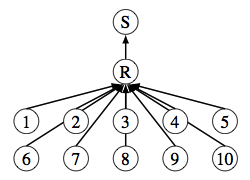
\includegraphics[width=5.5cm]{images/ch5-virtual-pan-test-1.png}
\flcaption{Schéma fonctionnel de notre PAN virtuel de test.\\
(Légende~: \textbf{R}~= noeud routeur~; \textbf{S}~= ``sink'')}
\label{FigVirtualPAN1}
\end{figure}


\newcommand{\nodeid}[1]{\textsf{#1}}


Nos premiers tests ont fait fonctionner le routeur et les dix noeuds simples
exclusivement sous le protocole S-CoSenS \cite{KR-SENSORNETS-2015}. Le but
de ces premiers essais était de vérifier la précision de la synchronisation
entre les différents appareils composant le PAN.

Cooja simule ici un médium radio <<~idéal~>>, sans bruit, affaiblissement
ou autres problèmes survenant en réel. Tous les noeuds sont à la portée
les uns des autres, sans zone d'ombre.

Ces tests ont clairement montré une excellente synchronisation entre les
noeuds-feuilles et le routeur, grâce à la granularité temporelle très fine
du système de gestion des évènements de RIOT OS (et plus particulièrement
la possibilité d'utiliser directement les différents \lang{timers} matériels
disponibles). Cette synchronisation peut être observée sur la copie d'écran
de notre simulation Cooja, visible en figure \vref{FigEcranCooja1}
\footnotemark[1].
Pour une meilleure lisibilité, la portion centrale de la fenêtre
\lang{``timeline''} (délimitée par un rectangle jaune épais) a été zoomée
en figure \vref{FigZoomTimelineCooja1}

\footnotetext[1]{\textbf{Note~:} bien que le titre de la figure
\vref{FigEcranCooja1} mentionne Contiki (dont le projet est à l'origine
du simulateur Cooja), les applications simulées fonctionnent bel et bien
sous RIOT OS.}


\begin{figure}[!p]
\raggedright
\begin{sideways}
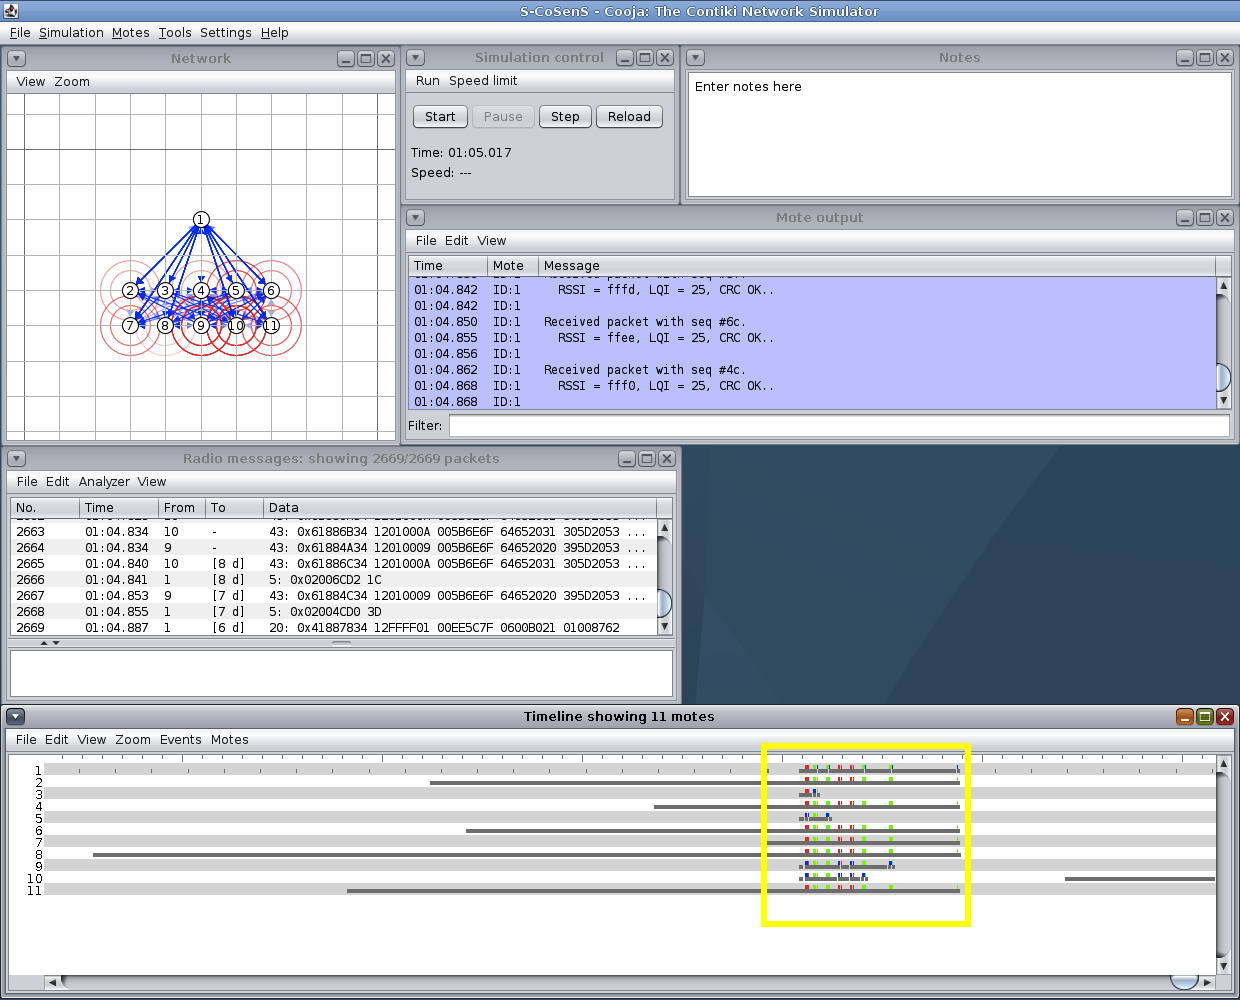
\includegraphics[width=17.4cm]{images/ch5-s-cosens-cooja-1.png}
\end{sideways}
\flcaption{Copie d'écran d'une des simulations de notre premier jeu de
tests sous Cooja.}
\label{FigEcranCooja1}
\end{figure}


\begin{figure}[pbt]
\centering
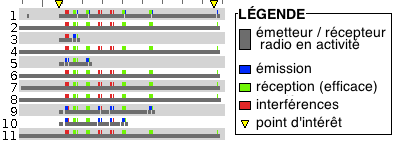
\includegraphics{images/ch5-s-cosens-timeline-1.png}
\flcaption{Zoom sur la partie centrale de la \lang{timeline} de la
figure \vref{FigEcranCooja1}.}
\label{FigZoomTimelineCooja1}
\end{figure}


Sur la figure \vref{FigZoomTimelineCooja1}, les nombres situés à gauche
représentent les identifiants numériques (ID) des \lang{motes}~: le routeur
possède l'ID numéro \nodeid{1}, tandis que les noeuds-feuilles ont les IDs
\nodeid{2} à \nodeid{11}. Les barres grises représentent les périodes
d'activité (écoute active ou transmission) de l'émetteur~/ récepteur radio
d'une \lang{mote} donnée. Les barres bleues représentent l'émission d'une
trame, et les barres vertes la réception \emph{réussie} d'une trame,
tandis que les barres rouges représentent des collisions (quand plusieurs
appareils émettent simultanément) et correspondent ainsi à la présence
sur le canal radio de signaux indéchiffrables.

La figure \vref{FigZoomTimelineCooja1} représente un court instant
(environ 100~millisecondes), correspondant à la fin d'un cycle radio du
routeur~: les 20 premières millisecondes correspondent à la fin de la
période  de sommeil SP (voir le mode de fonctionnnement de S-CoSenS en
section \vref{ParSCoSenS}), et les 80~millisecondes suivantes
représentent la période d'écoute WP, avant le début d'un nouveau cycle
radio (la période de retransmission TP du routeur ayant été désactivée
dans la simulation montrée sur ces copies d'écran pour une meilleure
lisibilité).

Dans l'exemple de la figure \vref{FigZoomTimelineCooja1}, quatre noeuds
ont des données à transmettre au routeur~: les \lang{motes} numéro \nodeid{3},
\nodeid{5}, \nodeid{9} et \nodeid{10}~; les autres noeuds (\nodeid{2},
\nodeid{4}, \nodeid{6}, \nodeid{7}, \nodeid{8} et \nodeid{11}) se préparent
eux à transmettre une trame durant le cycle suivant.

À l'instant marqué par la première flèche jaune (en haut à gauche de la
figure \vref{FigZoomTimelineCooja1}), la période de sommeil SP se
termine et le routeur active son émetteur~/ récepteur radio pour entrer
en période d'écoute WP. On notera que les quatre noeuds ayant des trames
à émettre (\nodeid{3}, \nodeid{5}, \nodeid{9} et \nodeid{10}) activent
également leur radio \emph{précisément} au même instant (à un \lang{tick}
de \lang{timer} soit environ 30 microsecondes près)~: ceci grâce à la
précision des mécanismes temps-réel de RIOT OS (basé sur les \lang{timers}
matériels), permettant aux différents noeuds de se synchroniser précisément
sur les valeurs temporelles transmises par le routeur dans le précédent
\lang{beacon} de début de cycle. Grâce à ce même mécanisme, les noeuds
sont capables de passer leur émetteur~/ récepteur radio \emph{et} leur
microcontrôleur en mode basse consommation aux moments adéquats,
le noyau de RIOT OS étant piloté par les interruptions.

Durant la période d'écoute, nous voyons également que plusieurs collisions
se produisent~; celles-ci sont résolues par la méthode CSMA/CA (sur laquelle
est basé S-CoSenS), laquelle oblige les \lang{motes} à attendre un délai
aléatoire avant de réémettre une trame en cas de conflit. Dans cet exemple,
nos quatre noeuds-feuilles peuvent finalement transmettre leur trame au
routeur dans cet ordre~: \nodeid{3} (après une première collision),
\nodeid{5} et \nodeid{10} (après deux autres collisions), et finalement
\nodeid{9}.

Notons que chaque fois que le routeur (ID numéro \nodeid{1}) reçoit une
trame avec succès, un acquittement (ACK) est renvoyé à l'émetteur~: cela
correspond aux barres bleues très fines suivant chaque barre verte sur
la ligne numéro \nodeid{1}.

Finalement, à l'instant marqué par la seconde flèche jaune (en haut à droite
de la figure \vref{FigZoomTimelineCooja1}), la période d'écoute WP
s'achève, et un nouveau cycle commence. En conséquence, le routeur émet un
\lang{beacon} contenant les durées calculées pour les différentes
périodes constituant le nouveau cycle, et qui serviront à la synchronisation
des dix noeuds-feuilles avec le routeur.

Il est à noter que les \lang{beacon}, contrairement aux trames
de données, ne font pas l'objet d'une transmission classique avec un ou
plusieurs destinataire(s) désigné(s) (\lang{``unicast''} ou
\lang{``multicast''}), mais sont émis pour réception par tous les noeuds
à portée d'écoute~: on dit que les \lang{beacons} font l'objet d'une
diffusion (\lang{``broadcast''}). Par conséquent, contrairement aux trames
de données, les \lang{beacons}~--- étant diffusés~--- ne font pas l'objet
d'un acquittement après réception.

Nous pouvons voir que tous les six noeuds attendant de transmettre une
trame durant ce nouveau cycle (\nodeid{2}, \nodeid{4}, \nodeid{6},
\nodeid{7}, \nodeid{8} et \nodeid{11}) se mettent en sommeil (leur
radio et leur microcontrôleur passent en mode basse consommation) juste
après avoir reçu le \lang{beacon}~; comme nous le voyons dans la figure
\vref{FigZoomTimelineCooja1}, ils vont profiter de la précision des
fonctionnalités temps réel de RIOT pour se réveiller précisément quand
le routeur passera en période d'écoute WP et sera ainsi prêt à recevoir
leurs trames.

%%%%%%%%%%%%%%%%%%%%%%%%%%%%%%%%%%%%%%%%%%%%%%%%%%%%%%%%%%%%%%%%%%%%%%%%%%%%%

\section[\'Evaluation des performances~: comparaison avec ContikiMAC]
        {\'Evaluation des performances~: comparaison avec \\
           ContikiMAC}
\label{SecEvalPerfSCosens}

Après avoir ainsi validé (de façon théorique) la fiabilité de notre
implantation de S-CoSenS sous RIOT, nous avons comme prévu lancé des
simulations pour la comparer avec l'implantation standard de ContikiMAC
sous Contiki OS \cite{KR-RR-8777-2015}.


\subsection{Configuration des expériences}
\label{SubsecCfgExp2}

Nous avons continué à effectuer des simulations sur le même PAN virtuel
montré en figure \vref{FigVirtualPAN1}. Nous avons cette fois
programmé des applications de test équivalentes sous Contiki (avec
ContikiMAC) et RIOT OS (avec S-CoSenS), effectuant des scénarios similaires
au premier~: les dix noeuds-feuilles envoient des trames au routeur, qui
les retransmet au \lang{sink} jouant le rôle de destination finale des
trames. Ces modalités de transfert sont statiquement programmées, aucun
protocole de routage n'étant utilisé~: nous testons ici uniquement les
protocoles MAC~/ RDC, et non des piles complètes.

Notre second type de simulations a consisté à faire varier le trafic réseau,
générant des charges allant d'un encombrement modéré à un trafic extrême.
Nous avons ainsi cherché à tester le comportement de ces protocoles MAC~/
RDC face à des charges réseau élevées, largement supérieures au trafic
habituellement traité dans les réseaux de capteurs sans-fil actuels.

Ces charges réseau sont générées par l'application de test s'exécutant
sur les dix noeuds-feuilles. Elle a été programmée pour générer des
trames 802.15.4 de grande taille~: 90 octets de charge utile, ce qui
correspond à une taille de trame physique de 110 octets. Les trames
sont envoyées de façon à respecter un intervalle d'arrivée de trames
(\lang{``Packet Arrival Interval''} ou PAI) moyen, en envoyant les
trames suivant un intervalle fixe modulé par un décalage aléatoire
pouvant atteindre la moitié du délai voulu~--- l'intervalle entre l'envoi
de deux trames consécutives est donc aléatoirement choisi entre
$[0,5\,\mathrm{PAI}\;;\;1,5\,\mathrm{PAI}]$~--- pour limiter les collisions
entre noeuds.

Les différentes configurations sont décrites en
table~\vref{TabConfigExp2}~: cette table donne le PAI moyen souhaité,
le nombre moyen de trames émises chaque seconde par l'ensemble des dix
noeuds-feuilles, et le débit réseau résultant attendu.


\begin{table}[htb]
\centering
\begin{tabular}{|l|r|r|r|}
\hline
Configuration & PAI moyen & Trames/s & Débit attendu \\
\hline
Modéré        &  1500 ms  &     6,7   &   5867 bit/s \\ 
\'Elevé       &  1000 ms  &    10     &   8800 bit/s \\
Très élevé    &   500 ms  &    20     &  17600 bit/s \\
Extrême       &   100 ms  &   100     &  88000 bit/s \\
\hline
\end{tabular}
\flcaption{Débits réseaux utiles programmés sur l'ensemble
des noeuds-feuilles.}
\label{TabConfigExp2}
\end{table}


En considérant la surcharge occasionnée par la couche MAC~/ RDC, le chemin
de transmission en deux étapes~--- ce qui signifie que le noeud routeur,
à un moment donné, doit communiquer soit avec les noeuds-feuilles, soit
avec le \lang{sink}~; ce qui revient à diviser effectivement la bande
passante du réseau par deux~---, la grande taille de nos trames de données
802.15.4 (proche du maximum physique de 127 octets), nous nous attendons
à ce que notre scénario <<~très élevé~>> soit proche du débit maximal
effectif possible, et à ce que le scénario <<~extrême~>> soit largement
au-délà de la saturation du médium radio.


\subsection{Taux de réception des paquets}
\label{SubsecTRP}

Nous avons utilisé le taux de réception des paquets (TRP, en anglais PRR~:
\lang{Paquet Reception Rate}) au niveau du \lang{``sink''} comme premier
indicateur pour quantifier la qualité de service (QdS) obtenue par
les protocoles testés.

Nous avons ainsi pu déterminer que le seul paramètre commun aux deux
protocoles ayant une influence réelle sur le TRP est la longueur de la
\lang{subframe} sous S-CoSenS (cf. section \vref{ParSCoSenS}),
l'équivalent sous ContikiMAC étant l'intervalle de réveil (\lang{check
interval}, durée entre deux écoutes consécutives du médium radio,
cf. section \vref{ParContikiMAC}). Ces deux paramètres correspondent
en fait, dans leurs protocoles respectifs, à la longueur du cycle de
fonctionnement du protocole, et donc à la fréquence de renouvellement
de ces cycles au cours d'une seconde.

Cet intervalle est configuré, au niveau de l'implantation, en changeant
la fréquence à laquelle le médium radio est écouté~: ce paramètre, dans
le code source de Contiki, est une constante de compilation nommée
\texttt{NETSTACK\_CONF\_RDC\_CHANNEL \_CHECK\_RATE} donnée en Hertz.
Sa valeur par défaut est de 8, ce qui signifie que ContikiMAC écoute
cycliquement le médium radio pour détecter une activité huit fois
par seconde.

S-CoSenS offre également un autre paramètre permettant de régler finement
l'équilibre entre qualité de service et économie d'énergie (via la mise
en sommeil de la radio)~: il s'agit des valeurs $\mathrm{WP}_{min}$ et
$\mathrm{WP}_{max}$ dont le rôle est de borner le poids relatif de la
période d'attente WP au sein des cycles de S-CoSenS dans un intervalle
choisi par l'utilisateur. Plus spécifiquement, l'augmentation de la
valeur de $\mathrm{WP}_{min}$ permet de s'assurer que le TRP ne
descendra jamais en dessous d'un certain niveau. Pour nos simulations,
étant donné que nous souhaitons obtenir une QdS maximale, nous avons
systématiquement défini $\mathrm{WP}_{max} = \mathrm{PAI}$ et
$\mathrm{WP}_{min} = \frac{1}{2} \mathrm{PAI}$, PAI étant ici l'intervalle
moyen d'arrivée des packets souhaité pour la simulation donnée.

Notons également que nous avons permis, sous Contiki, à la couche MAC
CSMA~/ CA standard d'effectuer jusqu'à 7 tentatives de retransmissions
pour une trame donnée, en définissant la constante de compilation
\texttt{CSMA\_CONF\_MAX\_MAC\_TRANSMISSIONS} à 8 dans le code source
de Contiki. Ceci a été fait pour mettre Contiki sur un pied d'égalité
avec la configuration par défaut de S-CoSenS, dans laquelle une trame
peut tenter d'être transmis jusqu'à 8 fois avant d'être abandonné.
Attention toutefois~: le terme de <<~réessai~>> n'a pas la même sémantique
sous S-CoSenS~--- où un réessai signifie la réémission \emph{d'une instance}
d'une trame donnée~--- que sous ContikiMAC~--- où un réessai indique
\emph{un nouveau cycle} durant lequel la trame sera réémise un nombre
de fois indéterminé. Cette différence de signification est la conséquence
des conceptions totalement différentes entre les deux protocoles,
comme cela a été décrit dans la section \vref{SecProtoMAC} décrivant
l'état de l'art en matière de protocoles MAC.

La configuration par défaut de 8~Hz~/ 125~ms pour le \lang{channel check
rate} ne donne que des résultats médiocres pour ContikiMAC, cette valeur
n'ayant visiblement pas été prévue pour permettre à ce protocole de gérer
les lourdes charges réseau. Dans un souci d'équité, nous avons
successivement doublé ce paramètre à 16~Hz~/ 62~ms, puis à 32~Hz~/ 31~ms
pour retenter nos tests de comparaison.

\bigskip

Les résultats que nous avons obtenus pour le TRP (PRR dans la légende
des figures) sont montrés dans les figures \vrefrange{FigComparPRR8Hz}
{FigInstablPRRContikiMAC}. Ces figures montrent le taux de
paquets arrivés avec succès à leur destination, en fonction de la durée
du cycle sous S-ConSenS, ou du \lang{channel check rate} sous ContikiMAC.
Ces résultats sont obtenus avec des simulations envoyant toujours
un nombre total constant de trames~: 500 trames par noeud-feuille,
soit 5000 trames au total pour chaque simulation.

\begin{figure}[htb]
\centering
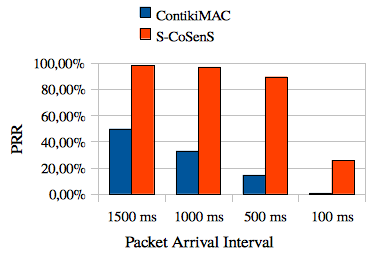
\includegraphics[width=8cm]{images/ch5-trp-8hz.png}
\flcaption{Résultats pour le taux de réception de paquets (PRR) pour un
cycle MAC~/ RDC de 8~Hz~/ 125~ms.}
\label{FigComparPRR8Hz}
\end{figure}

\begin{figure}[htb]
\centering
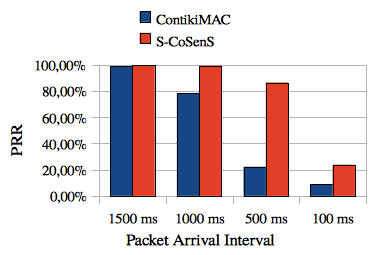
\includegraphics[width=8cm]{images/ch5-trp-16hz.png}
\flcaption{Résultats pour le taux de réception de paquets (PRR) pour un
cycle MAC~/ RDC de 16~Hz~/ 62~ms.}
\label{FigComparPRR16Hz}
\end{figure}

\begin{figure}[htb]
\centering
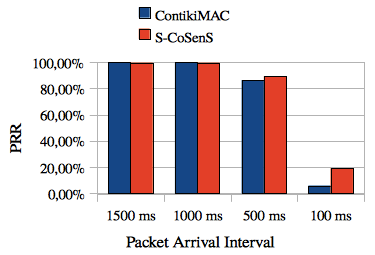
\includegraphics[width=8cm]{images/ch5-trp-32hz.png}
\flcaption{Résultats pour le taux de réception de paquets (PRR) pour un
cycle MAC~/ RDC de 32~Hz~/ 31~ms.}
\label{FigComparPRR32Hz}
\end{figure}

\begin{figure}[htb]
\centering
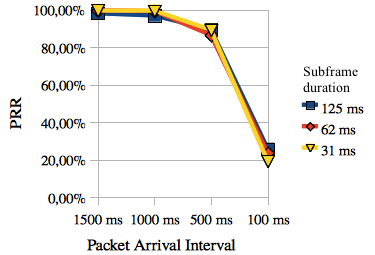
\includegraphics[width=8cm]{images/ch5-trp-stability-s-cosens.png}
\flcaption{Résultats combinés pour le taux de réception de paquets (TRP)
avec S-CoSenS, en fonction de la durée de la \lang{subframe}.}
\label{FigStablPRRSCoSenS}
\end{figure}

\begin{figure}[htb]
\centering
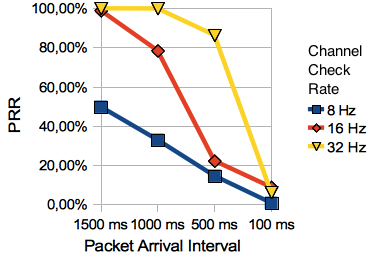
\includegraphics[width=8cm]{images/ch5-trp-unstability-contikimac.png}
\flcaption{Résultats combinés pour le taux de réception de paquets (TRP)
avec ContikiMAC, en fonction du \lang{channel check rate}.}
\label{FigInstablPRRContikiMAC}
\end{figure}

Les données représentées dans les figures \vrefrange{FigComparPRR8Hz}
{FigInstablPRRContikiMAC} nous montrent les faits suivants~:

\begin{itemize}

\item Le TRP de ContikiMAC augmente de façon significative avec le
\lang{channel check rate}, c'est-à-dire~: quand cet intervalle de
\lang{channel check rate} diminue, aboutissant à des cycles plus courts
et des écoutes plus fréquentes du médium radio.

\item Le TRP de S-CoSenS est toujours soit similaire, soit supérieur
à celui de ContikiMAC, quel que soit le scénario observé.

\item Le TRP de S-CoSenS reste très stable quelle que soit la valeur
donnée à la durée du cycle (\lang{subframe})~: cette stabilité est
clairement visible en figure \vref{FigStablPRRSCoSenS}. À l'inverse,
la figure \vref{FigInstablPRRContikiMAC} montre nettement que le TRP
de ContikiMAC varie énormément en fonction du \lang{channel check rate},
celui-ci devant être quadruplé (par rapport à sa valeur par défaut)
pour obtenir des résultats comparables à S-CoSenS.\\
Par conséquent, il est clair que les performances de S-CoSenS, en
matière de TRP, sont clairement plus prévisibles, et permettent de
s'assurer que le TRP restera dans des valeurs correctes ($> 80\%$)
dans la plupart des situations~--- c'est-à-dire tant que le médium
radio n'est pas complètement saturé comme dans le cas de notre
scénario <<~extrême~>>.

\end{itemize}

L'analyse détaillée des résultats des simulations, notamment le nombre
de retransmissions nécessaires pour chaque trame arrivé à destination,
nous montre également que~:

\begin{itemize}

\item avec ContikiMAC, les pertes de trames sont principalement dues
au routeur~;

\item avec S-CoSenS, le routeur ne perd jamais les trames qu'il a
reçus, toutes les pertes ont lieu lors des transmissions entre les
noeuds-feuilles et le routeur.

\end{itemize}

Cela n'est pas surprenant, car S-CoSenS réserve explicitement une période
de transmission (TP) durant chaque cycle exécuté par le routeur, pour
permettre à ce dernier de retransmettre les trames reçues dans les
meilleures conditions possibles. ContikiMAC ne possède lui aucune
fonctionnalité équivalente.

Durant ces périodes de transmission, une <<~priorité probabilistique~>>
est donnée par le protocole S-CoSenS aux routeurs, en leur accordant un
intervalle de base inférieur pour le calcul des périodes de \lang{backoff}
(il s'agit du paramètre nommé \emph{macMinBE} par le standard IEEE 802.15.4)
par rapport aux autres noeuds~: pour les routeurs $macMinBE = 2$, tandis que
pour les autres noeuds $macMinBE = 3$. Durant leurs périodes de transmission,
les routeurs sont ainsi privilégiés pour transmettre les trames présentes
dans leur file d'envoi.
Enfin et surtout, les noeuds-feuilles appartenant au même PAN qu'un routeur,
et ayant reçu ses \lang{beacons}, savent quand se déroule la période de
réception (WP) dudit routeur, et quand celle-ci s'achève pour laisser
la place à la période de transmission (TP). Les noeuds-feuilles appartenant
au même PAN que le routeur s'abstiennent alors de toute transmission,
remettant l'envoi des trames leur restant éventuellement à envoyer
au cycle suivant.

On peut clairement comprendre qu'au contraire, sous une forte charge
réseau, un routeur ContikiMAC va avoir des trames de données à recevoir
quasiment à chaque fois que celui-ci va sonder le médium radio
(\lang{``{Channel Check}''}) à chaque cycle. Ainsi, il va devenir de plus
en plus difficile pour ce routeur de trouver un intervalle disponible pour
l'envoi de ses propres trames au fur et à mesure que le trafic depuis les
noeuds-feuilles augmente. C'est pourquoi au cours de tels scénarios, le
noeud routeur devient clairement le point faible des PANs fonctionnant
sous ContikiMAC~; tandis que S-CoSenS peut éviter ces difficultés grâce
à sa conception, incluant une période de transmission (TP) réservée
à l'expédition des trames en attente dans la file d'envoi des routeurs.


\subsection{Délai total (<<~de bout-en-bout~>>) de transmission
            des trames}
\label{SubsecDelaiTransm}

Nous avons également calculé le délai que prend chaque trame transmise
avec succès pour aller de son noeud-feuille d'origine jusqu'au sink~---
c'est à dire la durée totale de son voyage en deux étapes
(\lang{``two-hop transmission''}). Ceci est le second indicateur de QdS
que nous avons étudié lors de ces expériences.

Les résultats que nous avons obtenus sont montrés dans les figures
\vrefrange{FigComparDelais8Hz}{FigInstablDelaisContikiMAC}.
Ces figures représentent les délais moyens nécessaires aux trames
transmises avec succès pour effectuer leur voyage en deux étapes. Notons que
les figures \vrefrange{FigComparDelais8Hz}{FigComparDelais32Hz}, pour des
raisons de lisibilité (tant la différence entre les résultats est énorme)
montrent les délais sur un axe vertical en échelle \emph{logarithmique}.

Contrairement aux résultats de TRP, ces résultats sont obtenus avec des
simulations où sont envoyés sans interruption des trames en nombre
indéfini, suivant là encore un intervalle moyen précalculé de transmission
entre deux trames consécutives. Le nombre de trames envoyées n'est donc
ici plus constant~; mais la charge générée sur le réseau reste fixée
de la même façon que pour les expériences sur le TRP.

\begin{figure}[htb]
\centering
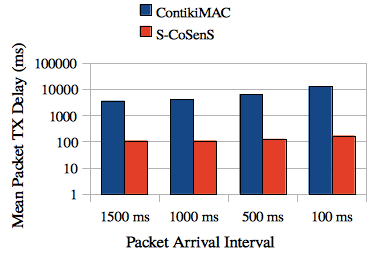
\includegraphics[width=8cm]{images/ch5-delays-8hz.png}
\flcaption{Résultats pour les délais moyens de transmission d'une trame
pour un cycle MAC~/ RDC de 8~Hz~/ 125~ms.}
\label{FigComparDelais8Hz}
\end{figure}

\begin{figure}[htb]
\centering
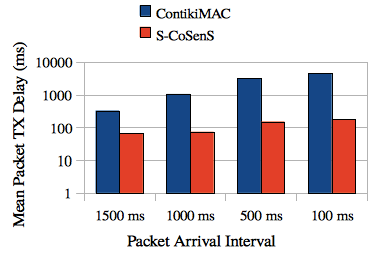
\includegraphics[width=8cm]{images/ch5-delays-16hz.png}
\flcaption{Résultats pour les délais moyens de transmission d'une trame
pour un cycle MAC~/ RDC de 16~Hz~/ 62~ms.}
\label{FigComparDelais16Hz}
\end{figure}

\begin{figure}[htb]
\centering
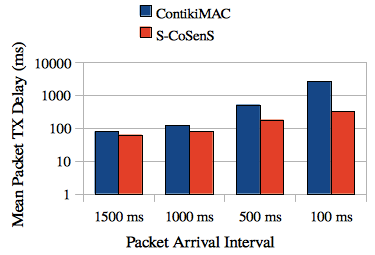
\includegraphics[width=8cm]{images/ch5-delays-32hz.png}
\flcaption{Résultats pour les délais moyens de transmission d'une trame
pour un cycle MAC~/ RDC de 32~Hz~/ 31~ms.}
\label{FigComparDelais32Hz}
\end{figure}

\begin{figure}[htb]
\centering
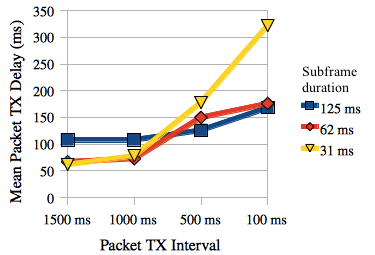
\includegraphics[width=8cm]{images/ch5-delays-stability-s-cosens.png}
\flcaption{Résultats combinés pour les délais moyens de transmission d'une
trame avec S-CoSenS, en fonction de la durée de la \lang{subframe}.}
\label{FigStablDelaisSCoSenS}
\end{figure}

\begin{figure}[htb]
\centering
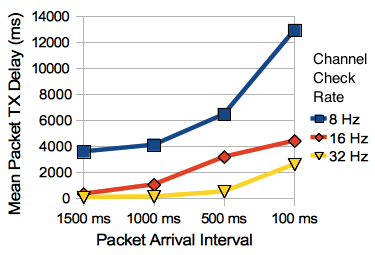
\includegraphics[width=8cm]{images/ch5-delays-unstability-contikimac.png}
\flcaption{Résultats combinés pour les délais moyens de transmission d'une
trame avec ContikiMAC, en fonction du \lang{channel check rate}.}
\label{FigInstablDelaisContikiMAC}
\end{figure}

\newpage

Ces résultats sur les délais de transmissions nous indiquent que~:

\begin{itemize}

\item Les délais de transmission sous ContikiMAC diminuent avec
l'augmentation du \lang{channel check rate}, c'est-à-dire~: quand 
les cycles ContikiMAC deviennent eux-mêmes plus courts.

\item Les délais de transmission sous S-CoSenS sont toujours soit
similaires, soit (dans la majorité des cas) nettement plus courts
que ceux de ContikiMAC, quel que soit le scénario observé.

\item Les délais de transmission sous S-CoSenS restent stables
quelle que soit la valeur donnée à la durée du cycle (\lang{subframe})~:
cette stabilité est clairement visible en figure
\vref{FigStablDelaisSCoSenS}. Dans la plupart des cas (c'est-à-dire
quand le médium radio n'est pas saturé), S-CoSenS permet de s'assurer
que les délais de transmission des trames resteront inférieurs à
une limite raisonnable (toujours $< 200$~ms, y compris dans les cas
les moins favorables).\\
À l'inverse, la figure \vref{FigInstablDelaisContikiMAC} montre
une instabilité énorme sous ContikiMAC dans les délais de transmission
en fonction des scénarios étudiés~: avec le réglage par défaut (8~Hz),
le délai de transmission des trames dépasse systématiquement et
largement le seuil de la seconde (plus de 12~secondes pour
transmettre une trame dans le cas le plus extrême).

\end{itemize}

On peut noter que ces trois observations (grande variabilité des résultats
de ContikiMAC, résultats similaires ou meilleurs pour S-CoSenS, stabilité
des résultats de S-CoSenS garantissant une QdS minimale) sont strictement
similaires à celles notées pour le taux de réception de paquets.

\bigskip

L'énorme augmentation dans les délais de transmission de bout-en-bout
pour ContikiMAC peut être interprétée comme un <<~excès de zèle~>>.
Une trame peut être transmise au cours d'un nombre prédéfini d'essais
(3~par défaut sous Contiki, 8~dans notre configuration par analogie
avec S-CoSenS). Rappelons que pour le couple ContikiMAC~-- CSMA/CA,
la transmission d'une trame peut être mise en attente jusqu'à la
disponibilité du médium radio, et qu'un <<~essai de transmission~>>
consiste à envoyer répétitivement cette trame jusqu'à concurrence
d'un cycle entier (durée calculée du \lang{channel check rate})~:
par conséquent, un délai énorme peut s'écouler avant que ce protocole
ne finisse par abandonner la transmission d'une trame donnée.

Si une telle <<~obstination~>> peut (en théorie) améliorer le TRP en
augmentant les chances de réception d'une trame par son destinataire,
elle finit par allonger de façon considérable le délai moyen pour la
transmission d'une trame de bout-en-bout. Au final, on peut s'interroger
sur l'utilité de continuer à chercher à transmettre des trames ayant
atteint un tel âge (dont les données risquent de devenir obsolètes),
souvent au détriment de la transmission de trames plus récentes
contenant des données plus actuelles donc plus utiles.

La configuration du nombre d'essais à tenter pour la transmission
d'une trame donnés est~--- comme pour de nombreux autres paramètres~---
un équilibre optimal à trouver entre deux buts contradictoires~: on
souhaite atteindre un TRP maximal, tout en permettant la perte et
l'élimination des trames trop âgées dont les données ont vraisemblablement
perdu leur intérêt. Il apparaît que dans les différents scénarios que nous
avons étudié, S-CoSenS permet d'obtenir un meilleur compromis entre
ces deux objectifs que ContikiMAC.


\subsection{Consommation d'énergie~: \lang{``Duty Cycles''}}
\label{SubsecDutyCycles}

Cooja peut facilement calculer les statistiques précises de \lang{``duty
cycle''}~--- ou pour être plus exact~: la fraction de temps pendant laquelle
les émetteurs~/ récepteurs radio sont actifs~--- pour chacune des
\lang{motes} virtuelles émulées. Ces statistiques sont un indicateur
très significatif pour quantifier les consommations d'énergie dans un
réseau de capteurs sans-fil, l'émetteur~/ récepteur radio étant, et de
loin, le circuit le plus gourmand en énergie au sein d'une \lang{mote}.

Les résultats obtenus pour les statistiques de \lang{duty cycle}
sont présentés dans les tables \vrefrange{TblDutyCyclesContikiMAC}
{TblDutyCyclesSCoSenS}. Notons qu'à cause des différences
importantes de TRP pour les durées de cycle de 125 et 62~ms, seule
la comparaison des résultats de \lang{duty cycle} pour des cycles de
31~ms avait un sens~; ce sont donc les seuls résultats que nous
présentons ici.

Dans ces deux tables, les lignes <<~activité radio~>> indiquent le
pourcentage du temps de simulation durant lequel l'émetteur~/ récepteur
accède activement au médium, et consomme donc de l'énergie.
Parmi ce temps d'activité, on distingue~:
\begin{itemize}
\item la fraction de temps durant laquelle le noeud émet avec succès
des trames de données (lignes <<~transmission efficace~>>)~;
\item la fraction de temps durant laquelle le noeud reçoit avec succès
des trames de données (lignes <<~réception efficace~>>)~;
\item la fraction de temps durant laquelle plusieurs noeuds émettent
simultanément, conduisant à la présence de signaux indéchiffrables sur
le médium radio (lignes <<~interférences~>>, qui couvrent en fait toutes
les émissions sans succès)~;
\item le temps d'activité radio n'étant pas couvert par ces trois
états précédents correspondent à des écoutes <<~à vide~>> du canal radio.
\end{itemize}


%%% ContikiMAC duty cycles
\begin{table}[htbp]
\centering
\begin{tabular}{|l|r|r|r|}
\hline
\multicolumn{4}{|c|}{ContikiMAC~: \lang{Channel Check Interval} = 32~Hz}\\
\hline
\multicolumn{4}{|r|}{INTERVALLE D'\'EMISSION DES TRAMES}\\
\hline
 & 1500 ms & 1000 ms & 500 ms \\
\hline
ROUTEUR                    & \multicolumn{3}{|c|}{ }\\
\hline
Activité radio             & 12,77\% & 17,85\% & 31,13\% \\
Transmission efficace      &  2,64\% &  4,00\% &  6,88\% \\
Réception efficace         &  2,78\% &  4,18\% &  8,24\% \\
Interférences              &  0,16\% &  0,40\% &  2,64\% \\
\hline
 NOEUDS-FEUILLES (moyenne) & \multicolumn{3}{|c|}{ }\\
\hline
Activité radio             &  5,61\% &  7,45\% & 14,27\% \\
Transmission efficace      &  0,90\% &  1,48\% &  3,89\% \\
Réception efficace         &  0,66\% &  1,03\% &  1,96\% \\
Interférences              &  0,11\% &  0,21\% &  1,13\% \\
\hline
\end{tabular}
\flcaption{Statistiques de \lang{duty cycle} pour ContikiMAC.}
\label{TblDutyCyclesContikiMAC}
\end{table}


%%% S-CoSenS duty cycles
\begin{table}[hbtp]
\centering
\begin{tabular}{|l|r|r|r|}
\hline
\multicolumn{4}{|c|}{S-CoSenS~: Durée d'un cycle (\lang{subframe}) = 31~ms}\\
\hline
\multicolumn{4}{|r|}{INTERVALLE D'\'EMISSION DES TRAMES}\\
\hline
 & 1500 ms & 1000 ms & 500 ms \\
\hline
ROUTEUR                    & \multicolumn{3}{|c|}{ }\\
\hline
Activité radio             & 66,22\% & 67,56\% & 67,91\% \\
Transmission efficace      &  4,96\% &  5,48\% &  8,43\% \\
Réception efficace         &  3,84\% &  4,43\% &  8,90\% \\
Interférences              &  1,04\% &  1,48\% &  8,39\% \\
\hline
 NOEUDS-FEUILLES (moyenne) & \multicolumn{3}{|c|}{ }\\
\hline
Activité radio             &  6,15\% &  7,68\% & 40,04\% \\
Transmission efficace      &  0,58\% &  0,70\% &  2,64\% \\
Réception efficace         &  0,68\% &  0,93\% &  7,08\% \\
Interférences              &  0,16\% &  0,22\% &  3,98\% \\
\hline
\end{tabular}
\flcaption{Statistiques de \lang{duty cycle} pour S-CoSenS.}
\label{TblDutyCyclesSCoSenS}
\end{table}


Les statistiques de \lang{duty cycle} présentées dans les tables
\vrefrange{TblDutyCyclesContikiMAC}{TblDutyCyclesSCoSenS} indiquent de
façon évidente que ContikiMAC possède sur ce terrain un avantage
très significatif. Les taux d'activité radio, que ce soit en émission,
en réception, ou en attente, sont toujours plus faibles~--- c'est à dire
meilleurs~--- pour ContikiMAC que pour S-CoSenS. Cela est particulièrement
vrai pour l'activité radio globale sur les noeuds routeurs, où la
différence en faveur de ContikiMAC est proprement spectaculaire.
(Cette différence est surtout due à la nécessité de fixer
$\mathrm{WP}_{min}$ à 50\% pour estimer correctement le trafic radio~---
cf. section \vref{SubSecPropoAlgo}.)
Ces constatations sont illustrées par les figures
\vrefrange{FigDutyCyclesRouteurs}{FigDutyCyclesFeuilles}.


%% figures de comparaison des "duty-cycles" pour les routeurs
\begin{figure}[htbp]
\centering
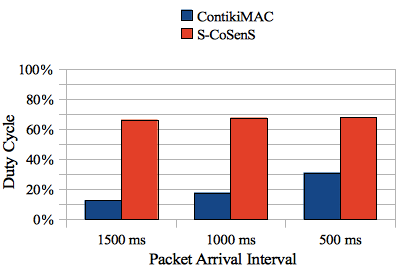
\includegraphics[width=8cm]{images/ch5-duty-cycles-routeurs.png}
\flcaption{Comparaison de l'activité radio (\lang{duty cycle}) sur les
noeuds routeurs fonctionnant respectivement sous ContikiMAC et S-CoSenS,
avec des \lang{subframes} de 31~ms.}
\label{FigDutyCyclesRouteurs}
\end{figure}


%% figures de comparaison des "duty-cycles" pour les noeuds-feuilles
\begin{figure}[htbp]
\centering
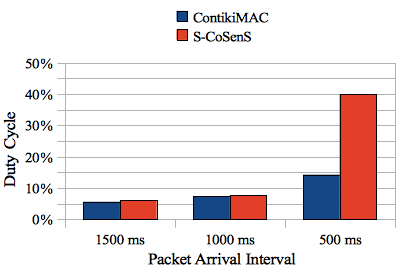
\includegraphics[width=8cm]{images/ch5-duty-cycles-noeuds-feuilles.png}
\flcaption{Comparaison de l'activité radio (\lang{duty cycle}) sur les
noeuds-feuilles fonctionnant respectivement sous ContikiMAC et S-CoSenS,
avec des \lang{subframes} de 31~ms.}
\label{FigDutyCyclesFeuilles}
\end{figure}


ContikiMAC prouve ainsi qu'il est en effet \emph{un protocole à très
basse consommation d'énergie}.

\bigskip

La seule exception à cette constatation de supériorité générale de
ContikiMAC en matière de \lang{duty cycle} se situe dans les temps
d'émission (lignes <<~transmission efficace~>>)~: pour les
noeuds-feuilles~--- mais \emph{pas} pour les routeurs~--- les \lang{duty
cycles} sont systématiquement légèrement inférieurs (c-à-d. meilleurs)
pour S-CoSenS. Cela s'explique aisément par la conception de ces deux
protocoles~: S-CoSenS est conçu~--- pour les transmissions entre
noeuds-feuilles et routeur~--- sur le paradigme RI-LPP (cf. section
\vref{SubsecProtoMACLPP}), ce qui implique naturellement moins de
tentatives de transmissions de trames de données que pour ContikiMAC
qui est conçu sur le paradigme LPL (cf. section \vref{ParContikiMAC})~---
et plus spécifiquement sur l'envoi continu de trames de données entières
par l'émetteur jusqu'à acquittement par le destinaire.


\subsection{Stabilité et contraintes mémoire}
\label{SubsecStabl}

Durant le développement et l'évaluation de S-CoSenS, nous avons
fait face à plusieurs plantages, notamment lorsque nous avons tenté
d'utiliser de longues files d'envoi de trames. Ces plantages étaient
dûs aux débordements de la pile système qui empiétait sur l'espace mémoire
de cette file~: quand cette dernière était pleine, les données des trames
pouvaient ainsi écraser le contenu de la pile système (lorsque ladite pile
contenait une quantité de données dépassant son espace mémoire alloué),
aboutissant bien évidemment à des erreurs logicielles fatales.

Les plantages observés avec cette implantation de S-CoSenS sous RIOT sont
dûs à la quantité très limitée de RAM disponible pour les données (8~Ko)
dans le microcontrôleur MSP430 autour duquel est bâtie la \lang{mote}
Zolertia Z1. Ceci, combiné à l'absence d'unité de protection mémoire
(MPU) dans cette architecture matérielle, aboutit à la survenue de
problèmes de corruption mémoire silencieux et indétectables en temps
voulu.

Si l'utilisation de microcontrôleurs disposant d'une quantité de RAM plus
conséquente peut limiter la survenue de tels problèmes, la détection
systématique de ces derniers et leur traitement correct nécessite
l'un des mécanismes suivants~:

\begin{enumerate}

\item \emph{Un mécanisme matériel} destiné à détecter les accès mémoire
incorrects et à provoquer une exception au début de leur survenue, avant
leur réalisation effective, prévenant ainsi leurs conséquences~: au sein
d'un microcontrôleur, ceci est le rôle d'une \nom{MPU} (\lang{Memory
Protection Unit}). Certaines architectures (comme les ARM Cortex-M)
proposent en option une telle fonctionnalité. Celle-ci nous semble
indispensable pour la conception de systèmes destinés à offrir un niveau
minimal de sûreté de fonctionnement (\lang{``safe systems''}).

\medskip

\item Pour les architectures dépourvues de MPU, \emph{un système de
support logiciel} dont le rôle est de surveiller les valeurs de registres
critiques~--- tels que le pointeur de pile (\nom{SP}~: \lang{Stack
Pointer})~--- ne serait-ce que pour s'assurer que ces valeurs restent
comprises au sein d'intervalles autorisés.\\
Un tel mécanisme peut être implanté \emph{au niveau d'un système
d'exploitation} (FreeRTOS et RIOT fournissent une telle option)~;
mais ce mécanisme ne peut~--- sans le support matériel d'une MPU~--- que
vérifier et constater la présence ou non d'une violation d'espace mémoire,
et en aucun cas empêcher sa survenue et ses conséquences. En cas de problème,
la seule alternative possible reste d'arrêter le système, et de le faire
éventuellement redémarrer <<~à froid~>> (\lang{``hard reset''}).\\
Un moyen plus efficace serait \emph{d'ajouter automatiquement, au cours du
processus de compilation, des séquences de code de vérification,} notamment
pour surveiller l'évolution de la valeur du registre SP lors de l'entrée
dans un sous-programme ou~--- pour les environnements multitâches~---
lors d'un changement de contexte. Ces types d'évènements étant ceux
augmentant la taille de la pile, ils correspondent donc aux moments
où cette dernière risque de déborder de son espace réservé.
Il deviendrait alors possible (comme avec une MPU) d'implanter un
traitement spécifique préventif des erreurs mémoires, n'interrompant que
les tâches ou routines fautives, sans devoir arrêter le système entier.

\end{enumerate}

\bigskip

Pour nos présentes expérimentations, nous avons contourné le problème
en réduisant simplement la profondeur de notre file d'envoi de trames,
laissant ainsi une place suffisante à la pile système.

\bigskip

Notons enfin que ce problème n'est nullement spécifique à RIOT ni à aucun
système d'exploitation embarqué, mais peut toucher tous les OS fonctionnant
sur du matériel aux ressources limitées, et surtout dépourvu d'une MPU ou
d'un autre mécanisme matériel de protection de la mémoire. Citons par
exemple \cite{ContikiPort8051} où sont expliquées les difficultés de portage
de Contiki sur une plate-forme matérielle courante et aux ressources
limitées~: on y parle clairement des problèmes de débordement de pile
(voir par exemple la figure~1 de cette publication), et des optimisations
qui ont été nécessaires pour éviter ce problème.

La stratégie de conception de systèmes extrêmement peu gourmands en
ressources comme Tiny OS et Contiki est de pousser l'optimisation à
l'extrême pour limiter ces problèmes au maximum (sans pour autant pouvoir
garantir une fiabilité absolue).


\subsection{Influence de l'optimisation des implantations}
\label{SubsecOptim}

Lors de nos différents tests, nous avons constaté que les délais
observés pour charger les trames dans le \lang{buffer} d'envoi du
composant radio CC2420 étaient toujours significativement plus longs
sous RIOT OS que sous Contiki.

Nos investigations à ce sujet nous ont montré que ces importantes
différences de délai étaient dues à la façon dont la communication
sur le bus SPI~--- assurant le lien entre le microcontrôleur central
et l'émetteur~/ récepteur radio dans la \lang{mote} utilisée~--- est
gérée par le système d'exploitation. Sous RIOT OS, lorsqu'un octet est
transmis sur le bus SPI, le résultat de la transmission est toujours
attendu, en consultant les \lang{flags} indiquant le succès ou l'échec,
avant de transmettre l'octet suivant. À l'inverse, Contiki utilise une
procédure nommée \lang{``fast SPI write''} envoyant un octet sur le bus
SPI dès que ce dernier est disponible (c'est-à-dire que le registre
d'envoi de l'interface microcontrôleur du bus SPI est disponible en
écriture), sans attendre de connaître le résultat de la transmission
précédente (les \lang{flags} indiquant le résultat d'une transmission
prenant un certain temps pour se mettre à jour).

Si la solution utilisée par Contiki est clairement plus rapide, elle
est également peu sûre car incapable de détecter correctement un
problème pouvant survenir sur le bus SPI~; l'implantation de
RIOT est au contraire sûre, mais plus lente.

Il y a clairement ici un compromis entre optimisation des performances
et fiabilité. Pour le chargement du \lang{buffer} d'envoi de l'émetteur~/
récepteur radio CC2420, cela dépend en fait moins de l'OS lui-même que
des choix d'implantation pour le pilote du bus SPI.


\begin{table}[!htb]
\centering
\begin{tabular}{|l|r|r|}
\hline
Système / Pilote SPI &  \multicolumn{2}{|c|}{Délai chargement} \\
\hline
RIOT OS~/ Standard (Sûr)            & 89 ticks & 2716 $\mu$s \\ 
RIOT OS~/ \lang{``Fast SPI write''} & 36 ticks & 1099 $\mu$s \\
Contiki~/ \lang{``Fast SPI write''} & 14 ticks &  213 $\mu$s \\
\hline
\end{tabular}
\flcaption{Delais observés pour le chargement d'une trame de 110 octets
dans le \lang{buffer} d'envoi de la radio CC2420 d'une \lang{mote} Zolertia
Z1, en fonction de l'OS et de l'implantation du pilote SPI.}
\label{TblTXPktLoadDelays}
\end{table}


Nous avons implanté l'optimisation \lang{``fast write''} du pilote SPI
sous RIOT, et avons mesuré les différences de rapidité entre
les deux versions du pilote sous RIOT, ainsi qu'avec le pilote
standard de Contiki. Les résultats sont montrés en table
\vref{TblTXPktLoadDelays}.

Les délais dans la table \vref{TblTXPktLoadDelays} sont donnés
dans la deuxième colonne en \lang{``ticks''} de \texttt{rtimer/hwtimer}
\footnotemark[2], les deux s'incrémentant à la fréquence de 32768~Hz.
Le \lang{``tick''} est donc une unité de temps fixe égale à environ
30,5 microsecondes. Les valeurs correspondantes en microsecondes sont
données en troisième colonne pour plus de facilité.

\footnotetext[2]{Rappelons que \texttt{rtimer} est le mécanisme de gestion
de \lang{timer} matériel en temps réel de Contiki OS, dont nous avons décrit
les limitations en section \vref{SubsecContikiTempsReel}~; \texttt{hwtimer}
est le mécanisme équivalent, plus performant, que nous avons utilisé sous
RIOT OS. Cependant, comme nous l'avons vu en section \vref{SubsecRIOTOS},
\texttt{hwtimer} a depuis été remplacé par le module \texttt{xtimer}.}

Nous pouvons quoi qu'il en soit noter que la pénalité imposée à S-CoSenS
par le pilote SPI standard de RIOT ne l'a pas empêché d'obtenir des
performances supérieures en matière de QdS (tous les tests faits avec
RIOT décrits dans la présente section ayant été exécutés avec le
pilote SPI standard du système).

\bigskip

Notons par contre que, contre toute attente, les délais de chargement
obtenus par simulation sous Cooja~/ MSPSim, montrés en table
\vref{TblTXPktLoadDelays} diffèrent très largement de ceux obtenus
sur une \lang{mote} Zolertia Z1 réelle. Nous reviendrons en détail sur ce
phénomène dans la section \vref{SecLimInexactSimu} du prochain chapitre.

Ce phénomène étonnant nous a en outre poussé à tenter de reproduire,
au moins partiellement, nos expériences sur matériel réel. C'est le sujet
de la section \ref{SubsecExpMat} suivante.


\subsection{Comparaison avec essais sur matériel}
\label{SubsecExpMat}

En nous basant sur les résultats obtenus dans la présente section
\ref{SecEvalPerfSCosens}, nous avons constaté que S-CoSenS avait
l'avantage sur ContikiMAC concernant les critères de QdS (TRP et délais
de transmission). Inversement, ContikiMAC est supérieur à S-CoSenS
concernant les \lang{duty cycles} (et donc la consommation d'énergie).

Les précédentes expériences ont bien sûr leurs limitations, la principale
d'entre elles étant qu'il s'agit uniquement de simulations. Cela peut
entraîner des inexactitudes et, à l'extrême, des conclusions erronées,
comme nous le verrons ultérieurement en section \vref{SecLimInexactSimu}.

Pour tenter de valider ces résultats de simulations, nous avons effectué
quelques tests sur un ensemble de noeuds WSN430 d'IoT-LAB. IoT-LAB
\cite{IotLAB} est un banc d'essai matériel permettant d'effectuer des tests
à distance sur des milliers de \lang{motes} de différents types~; nous
en reparlerons plus largement au chapitre \vref{ChValidation}.

Les \lang{motes} WSN430 que nous avons utilisées sont similaires aux
TelosB~/ SkyMotes (elles sont notamment basées sur le MSP430F1611),
et non à la Zolertia Z1 (construite autour d'un MSP430F2617, cf. section
\vref{SecHWMSP430})~; les conditions d'expérimentation ne sont donc
pas strictement similaires, mais sont destinées à nous donner une idée
générale de la validité de nos simulations.

Nous avons repris un PAN dont la structure est similaire à celle présentée
en figure \vref{FigVirtualPAN1}. Bien évidemment, il s'agit désormais
dans ces nouveaux tests de matériel réel.

Nous nous sommes limités à deux jeux d'essais, consistant à tester
l'implantation de S-CoSenS sous RIOT, avec deux durées de \lang{subframe}~:
\begin{itemize}
\item une durée de \lang{subframe} égale à 125~ms, correspondant à la
configuration de nos premiers jeux de simulation~;
\item une durée de \lang{subframe} égale à 100~ms~--- donc intermédiaire
entre les deux premières valeurs simulées~--- pour essayer d'avoir une
idée de l'évolution en allant vers des valeurs de \lang{subframe}
inférieures, comme pour les simulations.
\end{itemize}

Les résultats que nous avons obtenus avec nos expériences sur matériel
réel pour les taux de réception de paquets sont présentés en figure
\vref{FigPRRIoTLAB}.

\begin{figure}[htb]
\centering
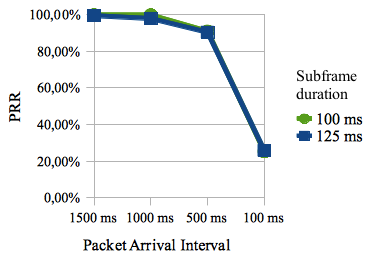
\includegraphics[width=8cm]{images/ch5-trp-iot-lab.png}
\flcaption{Résultats obtenus pour le taux de réception de paquets (TRP)
avec S-CoSenS, en fonction de la durée de la \lang{subframe}, sur des
\lang{motes} IoT-LAB WSN430.}
\label{FigPRRIoTLAB}
\end{figure}

\bigskip

On voit que les courbes présentées sont tout à fait similaires
à celles obtenues par simulation, telles que montrées dans la figure
\vref{FigStablPRRSCoSenS}, et semblent donc valider globalement
nos travaux et conclusions pour le TRP de notre protocole.

\smallskip

Concernant les délais de transmission, les résultats des expériences
sur matériel sont visibles en figure \vref{FigDelaisIoTLAB}.

\begin{figure}[htb]
\centering
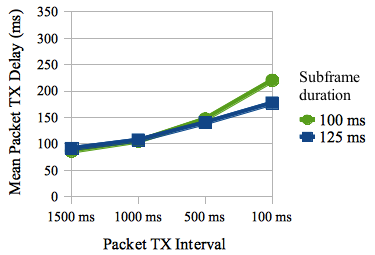
\includegraphics[width=8cm]{images/ch5-delays-iot-lab.png}
\flcaption{Résultats obtenus pour les délais moyens de transmission d'une
trame avec S-CoSenS, en fonction de la durée de la \lang{subframe}, sur
des \lang{motes} IoT-LAB WSN430.}
\label{FigDelaisIoTLAB}
\end{figure}

Notons ici que les délais, pour les simulations, étaient calculés très
précisément grâce à la fonction de relevé temporel des trames circulant
sur le média radio virtuel offerte par Cooja (fenêtre \lang{``Radio
messages''} et ses données exportables sous forme de fichier CSV).
Les motes WSN430 d'IoT-LAB ne possédant pas de \lang{``sniffers''}
de trames, les délais obtenus par ces tests sur matériel sont calculés
à partir de traces (\lang{``logs''}) de déboguage émises par les noeuds
utilisés lors de ces tests. Ces opérations d'écriture de traces (fonctions
de la famille \texttt{*printf()}) prenant elles-mêmes un certain temps
d'exécution, cela représente un biais supplémentaire entre ces expériences
sur matériel et nos simulations (en plus de la différence de
microcontrôleur).

Cela dit, les courbes nous montrent là encore des valeurs du même ordre
que celles obtenues par simulation en figure \vref{FigStablDelaisSCoSenS}.
Nos travaux et conclusions pour les délais de transmissions de notre
protocole semblent donc eux aussi valides.

\medskip

Nous n'avons par contre aucune donnée de \lang{``duty cycle''} issue de
ces expériences sur matériel à fournir, les motes WSN430 étant comme nous
l'avons dit dépourvues de l'instrumentation adéquate~--- alors que Cooja
fournit une fonction de calcul automatique de ces \lang{``duty cycles''}
via sa fenêtre \lang{``Timeline''}. Nous ne pouvons donc valider ou
invalider nos données simulées de \lang{``duty cycle''} via les présents
jeux d'expériences sur matériel.

%%%%%%%%%%%%%%%%%%%%%%%%%%%%%%%%%%%%%%%%%%%%%%%%%%%%%%%%%%%%%%%%%%%%%%%%%%%%%

\section{Améliorations potentielles des protocoles MAC~/RDC}
\label{SecAmeliorAlgoProtoMAC}


\subsection{Propositions d'améliorations algorithmiques}
\label{SubSecPropoAlgo}

Là encore, il s'agit de trouver un équilibre entre les deux objectifs
contradictoires que sont l'obtention d'une QdS maximale et de \lang{duty
cycles} minimaux. Par conception, ContikiMAC est clairement plus orienté
vers le second objectif que S-CoSenS, même s'il est possible de diminuer
la valeur du paramètre $\mathrm{WP}_{min}$ pour pousser notre protocole
à se rapprocher du même objectif. Cela est toutefois contraire à notre
politique consistant à donner la priorité absolue à la QdS.

Nous avons également, au cours de ces expériences, été amenés à réfléchir
sur les possibilités d'amélioration et d'optimisation de notre protocole
S-CoSenS, puis plus généralement de tout protocole MAC~/ RDC à haute
performance~:

\begin{enumerate}

\item En premier lieu, l'observation de ContikiMAC et de son fonctionnement
nous a poussé à \emph{tenter d'implanter un mécanisme similaire à
l'optimisation \lang{``phase lock''} de ContikiMAC (discutée en section
\vref{ParContikiMAC})} afin d'obtenir des \lang{duty cycles} inférieurs~---
c-à-d. meilleurs~--- pour les noeuds-feuilles fonctionnant sous S-CoSenS.

Les résultats de nos essais de simulation avec une telle optimisation se
sont révélés relativement concluants sous certaines conditions, comme
expliqué dans la section \ref{SubSecEvalAlgoSimu} suivante.

Plus qu'avec S-CoSenS, \emph{cette optimisation peut surtout être mise
à profit pour améliorer tout protocole asynchrone}, pour ajuster au mieux
les moments d'activation de la radio pour tenter d'émettre (protocoles LPL)
ou recevoir (protocoles LPP) des trames, \emph{si le protocole en question
possède une durée de cycle constante (ou au minimum prévisible).}

\smallskip

\item Une autre amélioration que nous avons imaginée pour S-CoSenS est
la suivante~: au lieu de compter le nombre de paquets retransmis par le
routeur durant les cycles précédents pour évaluer le trafic radio et
calculer la durée des périodes d'écoute WP (cf. section \vref{ParSCoSenS}),
nous souhaitons désormais nous servir du nombre de \nom{SFD} \footnotemark[3]
entendus durant les périodes d'écoute précédentes pour mieux évaluer
le trafic réseau passant et donc calculer plus justement les durées
des périodes d'écoute suivantes.

\footnotetext[3]{\nom{SFD~: \lang{``Start of Frame Delimiter''}}~;
il s'agit d'un signal radio (de contenu constant, prédéfini par la couche
physique du standard IEEE 802.15.4) envoyé sur le médium comme marqueur
pour signaler le début de l'émission d'une trame, et permettre la
synchronisation des récepteurs radio pour la bonne réception de cette
nouvelle trame.}

\smallskip

Comme nous l'avons vu dans la section \vref{ParSCoSenS} de l'état de l'art,
S-CoSenS (dans sa version actuelle) partage ses \lang{``subframes''} de
longueur fixe entre une période d'écoute WP et une période de sommeil SP.
Le calcul de la durée de WP est actuellement effectué sur la base du
nombre de trames reçues avec succès durant les périodes d'écoutes des
cycles précédents (via une moyenne glissante).

\smallskip

Ce mécanisme est efficace en théorie, mais ne tient pas compte du bruit.
Un réseau sans-fil peut être parasité par de nombreux facteurs
(interférences, collisions, ou même trames destinées à d'autres noeuds
surtout si plusieurs PANs différents sont présents à proximité).

En présence d'un tel bruit, les trames destinées à un noeud $N$ vont
être <<~noyées~>> dans la masse de signaux sans intérêt pour ce noeud $N$.
Par conséquent, avec le mode de calcul actuel, le noeud $N$, recevant peu
de trames utiles, va diminuer rapidement sa période d'écoute WP (passant
ainsi la majorité de ses cycles en période de sommeil SP). Il arrivera
alors, dans un milieu fortement bruité, que le noeud $N$ manque ainsi
des trames lui étant destinées. C'est pour cela que nous avons dû fixer
$\mathrm{WP}_{min}$ à 50\% sur les routeurs S-CoSenS lors de nos tests
(cf. section \vref{SubsecDutyCycles}) afin d'assurer une QdS suffisante.
(Nous donnons priorité absolue à la QdS~: voir la conclusion en section
\vref{SecDiscussContribConcluProtocolesMAC}).

Nous nous proposons, pour calculer la durée de WP, de ne plus compter le
nombre de trames reçues avec succès, mais de compter le nombre de SFD reçus,
c'est-à-dire le nombre de trames détectées sur le médium radio. Un tel
mode de calcul permet de tenir compte de tout le trafic <<~normal~>>
sans pour autant prendre en compte le <<~bruit brut~>> (interférences,
signaux non conformes au protocole IEEE 802.15.4)~; cela devrait ainsi
permettre à un noeud $N$ d'éviter de manquer des trames lui étant
destinées, pour cause de WP trop courte. Le défaut potentiel de cette
technique est d'augmenter la durée de WP, donc mécaniquement de diminuer
celle de SP, c'est-à-dire d'augmenter la consommation d'énergie du noeud,
peut-être inutilement. 

La contribution attendue de ces tests sur matériel réel est donc de
\emph{comparer les deux modes de calcul de la durée de WP~--- nombre
de trames reçues, et nombre de SFD détectés~--- et de déterminer par
l'expérience lequel représente le meilleur compromis} entre QdS (nombre
de trames reçues ou manquées) et consommation d'énergie (durée optimale
ou non de la période de sommeil SP).

Notons également que \emph{le recours aux SFD pour évaluer l'intensité
du trafic réseau peut être mis à profit pour améliorer tout protocole
ayant besoin de connaître cette intensité~--- ou même pouvant faire usage
de cette information~--- pour adapter dynamiquement son fonctionnement}.
ContikiMAC pourrait par exemple s'en servir pour faire varier de façon
dynamique son \lang{Channel Check Interval} en fonction du trafic,
l'augmentation de la fréquence de ce paramètre permettant visiblement
de mieux traiter les charges réseau intenses.

\item Nous avons également eu l'idée de combiner nos tests avec une
\emph{évaluation de l'influence du seuil de réception de l'émetteur~/
récepteur radio (\lang{``CCA Threshold''})}, telle qu'étudiée en détail
dans une publication de 2013 \cite{CCAThresholdStudy}~--- proposant un
protocole nommé \nom{AEDP} (\lang{``Adaptive Energy Detection Protocol''})
permettant d'améliorer la fiabilité des liens réseaux face au bruit
présent sur le médium radio~---, pour une éventuelle inclusion de la
gestion du \lang{``CCA Threshold''} dans la pile réseau de notre
plate-forme logicielle.

Le protocole AEDP décrit en \cite{CCAThresholdStudy} se penche sur
le problème du bruit, et de l'activité inutile des émetteurs~/ récepteurs
radio qui en découle.

Son principe est, pour résumer, d'adapter le seuil de sensibilité en dBm
de la radio (\lang{``CCA Threshold''}) en fonction de deux variables~:
le nombre d'envois nécessaires d'une trame donnée pour que celle-ci puisse
être transmise avec succès (variable ${ETX}$), et le nombre d'activations
de la radio nécessaires pour pouvoir détecter l'arrivée d'un signal utile
(variable ${WR}$). Le protocole AEDP consiste à ajuster le \lang{``CCA
Threshold''} (ici nommé variable $T$) tout en gardant $ETX$ en dessous
d'une valeur maximale d'essais pour réussir à envoyer une trame (constante
${ETX}_{threshold}$)~--- ce qui implique de diminuer $T$~---, \emph{et} en
évitant que $WR$ ne dépasse une valeur maximale correspondant au nombre
estimé nécessaire d'activations de la radio pour une réception correcte
(constante ${WR}_{threshold}$)~--- ce qui implique de d'augmenter $T$. \\
Pour résumer, le but du protocole AEDP est de trouver la valeur minimale
de $T$ telle que ${ETX} < {ETX}_{threshold}$ et ${WR} < {WR}_{threshold}$.
On voit qu'il s'agit, une fois de plus, d'un compromis entre QdS (taux
de réception de trames et débit de données: $ETX$) et consommation
minimale d'énergie ($WR$).

Ce protocole a au départ été conçu pour les protocoles LPL, dont le principe
est rappelons-le de se réveiller à intervalles (plus ou moins) réguliers
pour vérifier si une trame leur est destinée~--- cf. section
\vref{SubsecProtoMACLPL} de l'état de l'art~---, et a été testé
par ses auteurs sur TinyOS et Contiki.

Bien que S-CoSenS ne repose pas principalement sur LPL, le principe
consistant à jouer sur le \lang{``CCA Threshold''} pour améliorer le
rapport signal~/ bruit (\nom{SNR}~: \lang{Signal/Noise Ratio}) est
intéressant et peut être complémentaire, pour S-CoSenS, de l'essai
de la méthode du comptage des SFD pour optimiser le rapport QdS~/
consommation d'énergie.

On peut raisonnablement penser que \emph{l'adaptation dynamique du
\lang{``CCA Threshold''} pour améliorer le rapport signal~/ bruit peut être
mise à profit par n'importe quel protocole MAC~/ RDC~--- voire même plus
directement au niveau des pilotes radio eux-mêmes~--- pour améliorer les
performances et l'efficacité des transmissions sur les réseaux sans-fil}.

\end{enumerate}


\subsection{\'Evaluation de ces propositions~: difficultés et
            inadéquation des simulations}
\label{SubSecEvalAlgoSimu}

Il est naturel, pour tenter une première évaluation des trois
propositions d'améliorations algorithmiques détaillées dans la section
\ref{SubSecPropoAlgo} précédente, de songer à effectuer des simulations
utilisant des scénarios adéquats (notamment avec le \lang{framework} Cooja~/
MSPSim que nous avons déjà largement utilisé).

Toutefois, il s'avère que la mise en place de tels scénarios pour effectuer
des simulations~/ émulations valides est problématique, pour les raisons
suivantes~:

\begin{enumerate}

\item Concernant \emph{l'implantation d'un mécanisme similaire à
l'optimisation \lang{``phase lock''} de ContikiMAC}, notre but est
d'obtenir des données de \lang{``duty cycle''} afin de vérifier si des
améliorations significatives~--- c.-à-d. des valeurs d'activité radio
significativement inférieures~--- peuvent être obtenues. Or, comme nous
l'avons évoqué en section \vref{SubsecOptim}, et comme nous l'étudierons
en détail en section \ref{SecLimInexactSimu} au chapitre suivant, les
résultats (notamment de \lang{``duty cycle''}) obtenus à l'aide du
\lang{``framework''} Cooja~/ MSPSim manquent de fiabilité.
\emph{Les conclusions sur les éventuelles améliorations obtenues par
l'implantation du mécanisme de \lang{``phase lock''} via une étude faite
par simulations~/ émulations ne seront donc pas robustes, et pourront
facilement être remises en question}.

\item Concernant \emph{l'étude de l'influence des SFD sur le calcul de la
durée de la période d'écoute WP de S-CoSenS}, le matériel émulé par Cooja~/
MSPSim~--- à savoir les \lang{motes} Sky~/ TelosB tout comme les Z1~---
ne permet pas de recevoir l'interruption correspondant aux SFD (début de
réception d'une trame) de façon simple~: ces différentes \lang{motes}
relient en effet cette interruption à une entrée (\lang{``capture''}) d'un
des \lang{timers} du microcontrôleur central. Il faudrait pour la détecter
effectuer des modifications complexes et non portables au mécanisme de
gestion des \lang{timers} de RIOT, ce qui nuirait probablement à la
fiabilité de ce dernier. Une étude mettant en place une version ainsi
<<~altérée~>> de RIOT, d'une qualité insuffisante, n'aurait que peu
d'intérêt car ne pouvant fournir une implantation robuste et pérenne.
Il existe des \lang{motes} permettant de recevoir et gérer facilement
(du moins au niveau physique) les interruptions liées aux SFD, mais toutes
celles que nous connaissons sont des plates-formes matérielles basées sur
l'architecture ARM, pour laquelle aucun émulateur efficace n'est à l'heure
actuelle reconnu comme fiable, disponible et compatible avec Cooja.
\emph{Il nous est donc impossible d'émuler~--- du moins avec le
\lang{``framework''} Cooja~/ MSPSim que nous avons jusqu'ici utilisé~---
un matériel permettant de détecter les SFD de manière fiable et efficace.}

\item Concernant \emph{l'étude de l'influence du rapport signal~/ bruit
(SNR) sur l'optimisation de la qualité de service et la consommation
d'énergie}, une telle étude implique~--- par nature~--- le médium radio
de façon centrale. Or, il est bien connu que la simulation du médium radio
est le point faible de toutes les études par simulation des réseaux
sans-fil (qu'il s'agisse des WSN comme des réseaux plus <<~classiques~>>
comme le WiFi). En effet, comme nous l'avons vu notamment au chapitre
\ref{ChCtxProb}, le médium radio est par nature peu fiable, sujet à la
diffusion et présente des variations fortes et rapides~--- le plus souvent
imprévisibles~--- en fonction du temps et de l'espace. \emph{Des études
du SNR par simulation sont donc vouées à avoir une fiabilité, et donc
un intérêt, extrêmement limités.}

\end{enumerate}

\smallskip

\emph{Nous voyons donc que sur nos trois propositions d'améliorations
algorithmiques, les deux dernières ne peuvent pas être étudiées de façon
assez fiable par simulation~/ émulation}, et nécessiteront donc des études
sur des réseaux réels. Nous avons fourni une contribution mettant en place
la fonctionnalité de gestion du \lang{``CCA Threshold''} \cite{PRriotEnh13}
(nécessaire par exemple au protocole AEDP), qui pourra ainsi faire l'objet
de travaux ultérieurs idoines.

\smallskip

\emph{Concernant la première amélioration (\lang{``phase lock''}), une
étude par simulation, si elle n'offre pas une fiabilité satisfaisante,
est néanmoins possible pour tenter de se faire une première idée grossière
de l'efficacité d'une telle optimisation} (qui demandera bien sûr par la
suite confirmation par des tests sur matériel réel). Nous avons donc exécuté
un jeu de simulations, dans cette optique bien limitée d'exploration
préliminaire.

Nous avons repris le scénario d'émission de trames entre 10 noeuds-feuilles,
un routeur et un \lang{``sink''}, décrit et utilisé en section
\vref{SecEvalPerfSCosens}. Après avoir modifié notre implantation
de S-CoSenS pour tenter de synchroniser les noeuds-feuilles sur l'émission
des \lang{beacons} du routeur, nous avons relancé une série de tests et
obtenu les résultats de \lang{``duty cycle''} montrés en table
\vref{TblDutyCyclesSCoSenSPhaseLock}. La figure
\vref{FigDutyCyclesPhaseLock31ms} résume l'influence 
constatée du \lang{``phase lock''} au niveau de l'activité radio totale.


%% duty-cycles pour S-CoSenS "modifié"
\begin{table}[hbtp]
\centering
\begin{tabular}{|l|r|r|r|}
\hline
\multicolumn{4}{|c|}{S-CoSenS avec \lang{``phase lock''}~:
                     Durée d'un cycle (\lang{subframe}) = 31~ms}\\
\hline
 INTERVALLE D'\'EMISSION DES TRAMES & 1500 ms & 1000 ms & 500 ms \\
\hline
 NOEUDS-FEUILLES (moyenne) & \multicolumn{3}{|c|}{ }\\
\hline
Activité radio (protocole standard) &  6,15\% &  7,68\% & 40,04\% \\
Activité radio (avec \lang{``phase lock''})
                                    &  5,76\% &  7,03\% & 39,90\% \\
Transmission efficace               &  0,58\% &  0,70\% &  2,64\% \\
Réception efficace                  &  0,68\% &  0,93\% &  7,08\% \\
Interférences                       &  0,16\% &  0,22\% &  3,98\% \\
\hline
\end{tabular}
\flcaption{Statistiques de \lang{duty cycle} pour S-CoSenS avec optimisation
de type \lang{``phase-lock''} au niveau des noeuds-feuilles.}
\label{TblDutyCyclesSCoSenSPhaseLock}
\end{table}


%% figure de comparaison des duty-cycles pour S-CoSenS avec cycles courts
\begin{figure}[hbtp]
\centering
\includegraphics[width=14cm]{images/ch5-duty-cycles-pl-31ms.png}
\flcaption{Influence du mécanisme de \lang{``phase lock''} sur l'activité
radio (\lang{duty cycle}) induite par S-CoSenS, avec des \lang{subframes}
de 31~ms.}
\label{FigDutyCyclesPhaseLock31ms}
\end{figure}


On remarque que seules les données pour les noeuds-feuilles sont présentées~:
cette optimisation ne s'applique pas au routeur, du fait de la conception
même du protocole S-CoSenS.

On voit également que les valeurs de <<~transmission efficace~>>,
<<~réception efficace~>>, et <<~interférences~>> sont identiques à celles
de la table \vref{TblDutyCyclesSCoSenS}. Notre optimisation tente en effet
de réduire le temps d'écoute <<~à vide~>> des noeuds-feuilles, lors de
l'attente de réception des \lang{``beacons''}. Seules les valeurs de la
ligne <<~activité radio~>> varient donc par rapport aux résultats
du protocole S-CoSenS standard.

Ces valeurs <<~d'activité radio~>> totale sont effectivement moins élevées
par rapport au protocole S-CoSenS standard, mais la baisse de ces valeurs
reste relativement limitée, tout spécialement lors des forts trafics réseau~:
à un intervalle d'émission des trames de 500~ms, la baisse de valeur
d'activité radio est à peine perceptible. Ceci est logique~: dans une telle
configuration, la majorité de l'activité radio a lieu lors de la période
d'écoute du routeur (WP), et les nombreuses collisions sont responsables
de l'activité radio intense nécessaire pour pouvoir réussir à faire passer
les trames (nombreux réessais).

Avec des débits plus modérés (une trame toute les 1000 et 1500~ms),
la baisse est plus sensible, et permet de se rapprocher des (et même dans
un cas descendre sous les) valeurs d'activité radio constatées pour les
noeuds-feuilles sous ContikiMAC. Néanmoins, la baisse de valeur d'activité
radio due à la modification de S-CoSenS reste limitée~: étant donné que
S-CoSenS ne nécessite pas de répéter continuellement l'envoi des trames
jusqu'à réception par le destinataire (contrairement à ContikiMAC), on peut
être déçu de ne pas repasser systématiquement et surtout significativement
sous les valeurs d'activité radio de ContikiMAC.

\medskip

Nous avons retenté nos simulations, pour évaluer les \lang{``duty cycles''}
de ContikiMAC et S-CoSenS avec optimisation de type \lang{``phase-lock''},
cette fois avec une durée de cycle plus longue. Les résultats sont
visibles respectivement dans les tables
\vref{TblDutyCyclesContikiMACCycleLong} et
\vref{TblDutyCyclesSCoSenSPhaseLockCycleLong}, dans lesquelles nous
n'avons reporté que les valeurs des lignes <<~Activité radio~>> des
noeuds-feuilles, étant donné que nous avons vu que les autres valeurs
n'étaient pas affectées par cette optimisation. (Rappelons que dans cette
configuration~--- cycles de 125~ms~---, S-CoSenS obtient des résultats
largement meilleurs en termes de qualité de service que ContikiMAC,
comme vu dans les sections \vrefrange{SubsecTRP}{SubsecDelaiTransm}.)

Ces résultats sont également illustrés par la figure
\vref{FigDutyCyclesPhaseLock125ms}.


%%% duty cycles pour ContikiMAC avec cycle long
\begin{table}[htbp]
\centering
\begin{tabular}{|l|r|r|r|}
\hline
\multicolumn{4}{|c|}{ContikiMAC~: \lang{Channel Check Interval} = 8~Hz}\\
\hline
 INTERVALLE D'\'EMISSION DES TRAMES & 1500 ms & 1000 ms & 500 ms \\
\hline
 NOEUDS-FEUILLES (moyenne) & \multicolumn{3}{|c|}{ }\\
\hline
Activité radio             &  3,38\% &  3,87\% &  4,79\% \\
\hline
\end{tabular}
\flcaption{Statistiques de \lang{duty cycle} pour ContikiMAC avec un
cycle long~: CCI de 8~Hz (valeur par défaut), soit un cycle de 125~ms.}
\label{TblDutyCyclesContikiMACCycleLong}
\end{table}


%% duty-cycles pour S-CoSenS avec cycle long
\begin{table}[hbtp]
\centering
\begin{tabular}{|l|r|r|r|}
\hline
\multicolumn{4}{|c|}{S-CoSenS~:
                     Durée d'un cycle (\lang{subframe}) = 125~ms}\\
\hline
 INTERVALLE D'\'EMISSION DES TRAMES & 1500 ms & 1000 ms & 500 ms \\
\hline
 NOEUDS-FEUILLES (moyenne) & \multicolumn{3}{|c|}{ }\\
\hline
Activité radio (protocole standard) &  9,02\% & 11,45\% & 27,37\% \\
Activité radio (avec \lang{``phase lock''})
                                    &  4,61\% &  5,82\% & 17,26\% \\
\hline
\end{tabular}
\flcaption{Statistiques de \lang{duty cycle} pour S-CoSenS au niveau
des noeuds-feuilles, avec une \lang{subframe} longue de 125~ms.}
\label{TblDutyCyclesSCoSenSPhaseLockCycleLong}
\end{table}


%% figure de comparaison des duty-cycles avec cycles longs
\begin{figure}[htbp]
\centering
\includegraphics[width=14cm]{images/ch5-duty-cycles-pl-125ms.png}
\flcaption{Influence du mécanisme de \lang{``phase lock''} sur l'activité
radio (\lang{duty cycle}) induite par S-CoSenS et ContikiMAC, avec
respectivement des \lang{subframes} de 125~ms et des CCI de 8~Hz.}
\label{FigDutyCyclesPhaseLock125ms}
\end{figure}


On voit ici qu'avec une durée de \lang{subframe} plus longue,
le taux d'activité radio sous S-CoSenS baisse de façon significative avec
le mécanisme de \lang{``phase-lock''}~: de l'ordre d'un tiers d'activité
en moins avec un trafic réseau élevé (intervalle d'émission des trames de
500~ms), et une réduction de moitié de l'activité radio pour les charges
réseau plus modérées (intervalle d'émission des trames égal ou supérieur
à une seconde). Ce résultat est très intéressant, compte-tenu de la
supériorité de S-CoSenS du point de vue de la QdS dans cette situation.

Par contre, on voit que là encore, même si la baisse du pourcentage
d'activité radio devient importante au niveau de S-CoSenS avec une durée
de \lang{subframe} plus longue, ContikiMAC garde un \lang{duty cycle}
nettement inférieur.

\bigskip

Nous expliquons la relative importance des valeurs de \lang{duty cycle} 
de S-CoSenS~--- par rapport à ContikiMAC~--- de la façon suivante~:
outre la \lang{``subframe''} de longueur connue à l'avance, S-CoSenS
intègre dans son cycle une phase de transmission dont la durée reste
inconnue jusqu'à sa fin, puisque cette durée dépend du nombre de trames
à transmettre et du temps nécessaire pour les transmettre (éventuelles
interférences et collisions). Ainsi, S-CoSenS a toujours des cycles de
durée variable, tandis que l'intervalle entre deux cycles~--- c.-à-d.
deux CCA consécutifs~--- est toujours constant pour ContikiMAC quelles
que soient les circonstances (revoir les sections \vref{ParContikiMAC} et
\vref{ParSCoSenS} pour le détail du fonctionnement de ces deux protocoles).

Il est clair qu'un mécanisme du type \lang{``phase-lock''}, qui retient
la durée de cycle d'un récepteur pour optimiser les temps d'activation
des émetteurs, fonctionnera bien mieux avec un protocole à durée de cycle
constante comme ContikiMAC qu'avec un protocole auto-adaptatif comme
S-CoSenS ayant des cycles de durée variable et difficilement prévisible.

\bigskip

Ainsi, nous pouvons penser que~:

\begin{itemize}

\item \emph{l'implantation d'un mécanisme de type \lang{``phase-lock''}
se justifie pour S-CoSenS lorsqu'il est configuré avec une durée de
cycle (i.e.~: \lang{``subframe''}) suffisamment longue, là où les baisses
d'activité radio sont significatives, et de surcroît l'avantage de S-CoSenS
en termes de qualité de service est flagrant} (revoir sections
\vrefrange{SubsecTRP}{SubsecDelaiTransm})~;

\item par contre, \emph{la complexité supplémentaire introduite par l'ajout
d'un mécanisme de type \lang{``phase-lock''} au sein d'un protocole à durée
de cycle variable comme S-CoSenS ne se justifie guère lors de cycles
de fonctionnement (\lang{``subframes''}) courts, surtout en présence de
trafics réseau intenses, au vu des résultats forcément limités qu'apportera
dans de telles conditions un tel mécanisme} (à cause notamment de la grande
variabilité des durées de cycles)~;

\item \emph{un mécanisme de type \lang{``phase-lock''} devrait être assez
avantageux dans tous les cas pour envisager son implantation dans les
protocoles MAC~/ RDC à durée de cycle fixe et~/ ou connue à l'avance},
à condition bien sûr que la conception du protocole le permette.

\end{itemize}

%%%%%%%%%%%%%%%%%%%%%%%%%%%%%%%%%%%%%%%%%%%%%%%%%%%%%%%%%%%%%%%%%%%%%%%%%%%%%

\section[Discussion~: évaluation et comparaison de protocoles MAC~/ RDC,
         contributions et conclusion]
        {Discussion~: évaluation et comparaison de protocoles MAC~/ RDC,
         contributions et conclusion%
         \sectionmark{Discussion~: protocoles MAC~/ RDC,
                      contributions et conclusions}}
\sectionmark{Discussion~: protocoles MAC~/ RDC, contributions et conclusions}
\label{SecDiscussContribConcluProtocolesMAC}

Nos travaux ont permis de tester et comparer deux implantations complètes
et fonctionnelles de deux protocoles MAC~/ RDC, ContikiMAC et S-CoSenS.
Ces travaux ont consisté en des scénarios simulant de lourdes charges
réseau, dans le but d'observer la capacité de ces protocoles à monter
en charge, puis à les pousser dans leurs limites ultimes de fonctionnement~---
tout en sachant qu'approcher la limite théorique de 250~Kbit/s de bande
passante pour le médium radio physique défini par le standard IEEE
802.15.4 est impossible, à cause des délais imposés par le standard
lui-même (SIFS, LIFS), des limites matérielles des émetteurs~/ récepteurs
radio, et des délais occasionnés par les différentes couches des piles
réseau (et notamment les couches MAC et RDC).

Nous avons, durant l'implantation de S-CoSenS sur RIOT OS, surmonté
de nombreux problèmes dont nous avons discuté dans le présent chapitre.

Ce faisant, nous avons \emph{fourni les contributions suivantes}~:

\begin{itemize}

\item Nous avons d'abord \emph{prouvé que Cooja (le simulateur de WSN du
projet Contiki) n'était nullement limité à cette plate-forme logicielle}.
Nous l'avons employé avec succès pour tester des applications conçues sous
RIOT OS, et \emph{nous sommes convaincus que celui-ci peut servir à la
simulation de WSN fonctionnant avec n'importe quelle plate-forme logicielle,
ou même sans (programmation \lang{``bare metal''})}, et ce grâce au recours
à des émulateurs pour la gestion des \lang{motes} virtuelles.

\item Nous avons montré que des \emph{fonctionnalités temps-réel sont
nécessaires} pour implanter des protocoles MAC~/ RDC novateurs et
efficaces. Plus précisément~: une résolution temporelle à fine
granularité (nécessairement inférieure à la milliseconde, une résolution
de l'ordre de 30~microsecondes étant tout à fait satisfaisante), et la
disponibilité de plusieurs \lang{timers} offrant cette fine granularité
temporelle~--- l'usage d'au moins un \lang{timer} matériel étant en général
nécessaire pour atteindre un tel but.

\item Nous avons montré que \emph{notre implantation du protocole
S-CoSenS présente un avantage en termes de QdS} (TRP et délais de
transmissions) \emph{particulièrement en présence d'un trafic réseau
intense}, tandis que ContikiMAC (dans son implantation standard
sous Contiki) est largement supérieur en terme de \lang{duty cycles}.

\item Nous avons envisagé des \emph{contre-mesures pour gérer les erreurs
liées à des problèmes de corruption mémoire} (comme l'écrasement par
la pile système d'autres données, à cause de l'espace mémoire
très limité sur les \lang{motes} de base).
Notamment~--- sur les architectures matérielles dépourvues de circuit
MPU dédié~--- la nécessité de surveiller régulièrement la pile système,
\emph{de préférence par l'insertion automatique de code de vérification,
durant le processus de compilation,} à des endroits stratégiques du chemin
de code (appels de sous-programmes, interruptions, etc.).

\item Nous avons \emph{évalué l'influence des optimisations des
implantations sur les performances}, notamment dans la gestion du bus SPI,
selon le traitement des transmissions d'une façon sûre ou au contraire
optimisée~: le choix de l'une ou l'autre des solutions impacte la vitesse
de chargement des trames dans l'émetteur~/ récepteur radio d'un facteur
2 à 3, cette accélération se faisant au détriment de la fiabilité.
Notons toutefois que cette différence ne semble pas avoir changé
significativement les résultats globaux de nos comparaisons.

\item Nous avons enfin \emph{proposé des idées d'améliorations
algorithmiques au protocole S-CoSenS} (liées à l'optimisation des periodes
de réveil de l'émetteur~/ récepteur radio, à l'estimation du trafic réseau
et à l'optimisation du SNR), \emph{et à notre sens facilement généralisables
à de nombreux protocoles MAC~/ RDC}, si ce n'est~--- pour la dernière de
ces trois améliorations~--- à toutes les couches basses des piles réseau
des plates-formes logicielles destinées aux WSN.

\end{itemize}

En conclusion, nous avons constaté qu'il est essentiel pour un protocole
MAC~/ RDC d'être capable de traiter efficacement une lourde charge réseau
(ou des pointes de trafic), tout en gardant un \lang{duty cycle} minimal
durant les périodes de faible trafic.

Ces deux objectifs contradictoires doivent faire l'objet d'un compromis,
dont dépend le choix d'un protocole MAC~/ RDC et éventuellement la
configuration de celui-ci.

Notre conviction est toutefois qu'un WSN est \emph{d'abord} déployé pour
communiquer des informations, et doit donc \emph{en priorité} transmettre
le trafic réseau quand celui-ci apparaît. L'économie d'énergie est le
\emph{deuxième} objectif principal, pour allonger la durée de fonctionnement
et~/ ou de vie des noeuds du WSN, mais ne doit jamais~--- selon nous~---
se faire au détriment de la qualité de service <<~fonctionnelle~>>.

\emph{C'est pourquoi nous pensons qu'un protocole MAC~/ RDC idéal
est un protocole dont le \lang{``duty cycle''} doit varier dynamiquement
en fonction du trafic, certes pour permettre d'optimiser la consommation
d'énergie, mais jamais au prix de la perte de données à transmettre
(sauf bien sûr dans les cas de saturation du médium radio).}

\bigskip

Pour finir, rappelons que lors de nos tests concernant l'influence
de l'optimisation des implantations sur les performances (section
\vref{SubsecOptim}), nous avions observé des incohérences dans les
valeurs obtenues entre simulation et exécution sur matériel réel, tout
particulièrement en ce qui concerne la plate-forme matérielle Zolertia Z1.
Comme nous l'avions alors dit, nous allons maintenant étudier ce phénomène
en détail dans la section \ref{SecLimInexactSimu} du chapitre suivant.


%%%%%%%%%%%%%%%%%%%%%%%%%%%%%%%%%%%%%%%%%%%%%%%%%%%%%%%%%%%%%%%%%%%%%%%%%%%%%
%%%                 FIN DU CHAPITRE "PROTOCOLES MAC/RDC"                  %%%
%%%%%%%%%%%%%%%%%%%%%%%%%%%%%%%%%%%%%%%%%%%%%%%%%%%%%%%%%%%%%%%%%%%%%%%%%%%%%



%%% CHAPITRE 6 : VALIDATION
%%%%%%%%%%%%%%%%%%%%%%%%%%%%%%%%%%%%%%%%%%%%%%%%%%%%%%%%%%%%%%%%%%%%%%%%%%%%%%%%
%%%                               80 COLONNES                                %%%
%%%%%%%%%%%%%%%%%%%%%%%%%%%%%%%%%%%%%%%%%%%%%%%%%%%%%%%%%%%%%%%%%%%%%%%%%%%%%%%%

\chapter{Validation des expérimentations sur plates-formes réelles}
\label{ChValidation}

Le présent chapitre, dont le but est de valider les expériences effectués
jusqu'ici dans le cadre de la présente thèse, notamment au précédent
chapitre \ref{ChProtocolesMAC}, va consister en deux parties logiquement
liées et consécutives~:

\begin{enumerate}

\item Comme nous l'avons signalé en fin de section \vref{SubsecOptim},
nous avons constaté des incohérences entre nos simulations~/ émulations
effectuées sous Cooja, et des tests similaires effectués sur matériel réel
(ce qui nous avait déjà poussé à faire quelques premiers tests limités en
section \vref{SubsecExpMat}).

Ce phénomène d'incohérence va être étudié en détail dans la section
\ref{SecLimInexactSimu} suivante. Nous y verrons l'ampleur du problème,
ses causes probables, ses conséquences potentielles et, au final, nous
devrons ainsi reconnaître les limitations rendant les simulations
effectuées sous Cooja inadaptées aux travaux d'évaluation de performances~---
notamment liées aux temps et délais~--- de projets basés sur les WSN.

\item Partant de cette dernière conclusion, le reste de ce chapitre
sera consacré à des travaux de validation, consistant à reproduire nos
expérimentations simulées sur matériel réel, et plus précisément sur
un \lang{testbed} offrant un nombre suffisant de noeuds de WSN, dotés
de fonctionnalités d'instrumentation suffisantes pour recueillir
suffisamment facilement les données que Cooja permet d'obtenir sans
effort. La section \vref{SecObjectifs} décrira les travaux de validation
ainsi prévus, puis la section \vref{SecTravauxMiseOeuvre} détaillera les
problèmes techniques nous ayant rapidement empêché de mener à bien cette
campagne de tests de validation, fournissant autant que possible de détails
techniques dans l'espoir de permettre la poursuite de ces travaux et leur
réussite dans un effort, qui sera forcément ultérieur à la présente thèse.

\end{enumerate}

Ce chapitre sera enfin bien évidemment terminé par une section de
discussion et conclusion~: section \vref{SecConcluChValidation}.

%%%%%%%%%%%%%%%%%%%%%%%%%%%%%%%%%%%%%%%%%%%%%%%%%%%%%%%%%%%%%%%%%%%%%%%%%%%%%

\section{Motivation : limitations et inexactitudes des simulations}
\label{SecLimInexactSimu}

Cooja, le simulateur de réseaux de capteurs sans-fil du projet Contiki
(utilisant MSPSim pour l'émulation des noeuds MSP430 des réseaux),
est un outil très largement utilisé pour le développement et le déboguage,
mais aussi pour l'évaluation des performances des projets basés sur
les WSN.

Comme nous l'avons dit en section \vref{SubsecOptim}, nous avons observé
des incohérences temporelles entre simulations avec Cooja~/ MSPSim
(dans leurs versions fournies avec Contiki 2.7) et des essais similaires
effectués ensuite sur du matériel réel.

La table \vref{TblComparDelais} reprend les données de la table
\vref{TblTXPktLoadDelays}, en montrant cette fois les différences
constatées entre délais obtenus par simulation et délais obtenus par
expérimentation sur matériel réel (les valeurs sont toutes données en
\lang{``ticks''} de \lang{timers} matériels représentant environ
30,5~$\mu$s). Ces différences de délai, extrêmement élevées, n'ont
\lang{a priori} aucune raison rationnelle d'apparaître.

\begin{table}[!h]
\centering
\begin{tabular}{|l|r|r|}
\hline
Système / Pilote SPI                & Simu. Cooja  & Test matériel \\
\hline
RIOT OS~/ Standard (Sûr)            &   89 ticks   &  32 ticks \\ 
RIOT OS~/ \lang{``Fast SPI write''} &   36 ticks   &  14 ticks \\
Contiki~/ \lang{``Fast SPI write''} &   14 ticks   &   7 ticks \\
\hline
\end{tabular}
\flcaption{Delais observés par le chargement d'un paquet de 110 octets
dans le \lang{buffer} d'envoi de la radio CC2420 d'une mote Zolertia Z1,
en fonction de l'OS et de l'implantation du pilote SPI, par simulation
et par expérimentation sur matériel.}
\label{TblComparDelais}
\end{table}

De telles imprécisions pourraient remettre en cause l'utilisation de
Cooja~/ MSPSim comme outil d'évaluation, du moins pour les paramètres
liés aux performances temporelles \cite{KR-EWSN-NextMote-2016}.

Dans ce chapitre, après un bref rappel sur Cooja et MSPSim, nous détaillerons
les résultats de nos investigations, ainsi que les risques potentiels liés
à ce problème, et nous tenterons de donner des pistes pour le régler
ou du moins éviter ses conséquences.


\subsection{Rappels sur Cooja et MSPSim}
\label{SubsecCoojaMSPSim}

Fourni par le projet Contiki \cite{ContikiOS}, le simulateur \nom{Cooja}
\cite{Cooja} est devenu un outil très largement employé dans le domaine
des réseaux de capteurs sans-fil (WSN). La communauté académique l'emploie
notamment de façon intensive pour effectuer des simulations de réseaux
allant de différentes tailles~--- de quelques noeuds formant un unique PAN
comme dans nos expériences décrites en sections \vref{SecSCoSensRIOTPrecSync}
et \vref{SecEvalPerfSCosens}, à plusieurs centaines de \lang{motes} divisées
en de nombreux PANs interconnectés~---, lesquelles simulations permettent
de développer, déboguer et évaluer les performances des projets basés sur
l'une des technologie des WSN.

Le recours à de telles simulations est tout spécialement utile pour
effectuer des expérimentations sur des réseaux étendus et complexes,
contenant de nombreuses \lang{motes}~; réseaux qu'il serait long,
difficile et coûteux de mettre en oeuvre avec du matériel réel.

Cooja est en lui-même une application écrite avec le langage et la
plate-forme logicielle Java. Cette application offre trois fonctionnalités
principales~:

\begin{enumerate}

\item Une interface utilsateur graphique (GUI)~--- basée sur le jeu de
composants graphiques standard de Java (\lang{``Swing''})~--- permettant
de concevoir, d'exécuter et d'analyser des simulations de WSN.

\item La simulation du médium radio servant de support aux communications
sans-fil des réseaux de \lang{motes}. \\
Plusieurs modèles sont possibles, du médium <<~idéal~>>, au médium simulant
(aléatoirement) des interférences et autres pertes de signal, en passant par
un médium simulant uniquement un affaiblissement du signal proportionnel à
la distance à l'émetteur (modèle par défaut). Tous ces modèles incluent pour
chaque noeud la gestion d'une <<~portée utile~>> ainsi que d'une <<~zone
d'interférences~>>, les deux étant configurables par l'utilisateur.

\item Un \lang{framework} logiciel extensible, permettant l'intégration
d'outils externes amenant des fonctionnalités additionnelles à l'application
Cooja.

\end{enumerate}

C'est cette dernière fonctionnalité qui permet à Cooja d'émuler réellement
les différentes \lang{motes} constituant les WSN. En effet, Cooja embarque
et utilise~--- grâce à ce mécanisme~--- des programmes dédiés capables
d'effectuer l'émulation au cycle près (\lang{``cycle-exact emulation''})
des circuits intégrés avec lesquels sont contruites les \lang{motes}~:
microcontrôleurs (MCUs), émetteurs~/ récepteurs radio, etc.

Cette capacité d'émulation est l'un des principaux, sinon \emph{le}
principal point fort de Cooja~: grâce à l'émulation des \lang{motes},
des simulations extrêmement précises, de bas niveau et à granularité
très fine sont possibles. C'est cet avantage décisif qui a sans aucun
doute permis à Cooja de devenir l'outil de référence, tout spécialement
pour le déboguage et l'évaluation des applications tournant sur des noeuds
de réseaux de capteurs sans fil~--- applications tournant à l'heure actuelle
très souvent sous Contiki OS. Mais l'émulation précise du matériel permet
de faire tourner des programmes sous n'importe quelle plate-forme
logicielle, comme le prouvent les tests sous RIOT OS que nous avons
détaillés au chapitre \ref{ChProtocolesMAC}.

Les versions actuelles de Cooja embarquent et utilisent deux émulateurs
différents~: \nom{Avrora} \cite{Avrora} pour l'émulation des appareils basés
sur l'architecture Atmel AVR, et \nom{MSPSim} \cite{MSPSim} pour l'émulation
des appareils basés sur l'architecture MSP430 de Texas Instruments.

De ces deux émulateurs, MSPSim est actuellement le plus utilisé dans
les simulations Cooja décrites dans la littérature, étant donné que
les \lang{motes} basées sur des microcontrôleurs MSP430 sont les plus
fréquemment rencontrées et employées~: on citera notamment la famille
TelosB~/ Skymote, ou la plate-forme Zolerta Z1, que nous avons
décrites en section \vref{SecHWMSP430}, et qui font partie des
plates-formes matérielles supportées officiellement par Contiki OS.

Ces rappels étant faits, nous allons maintenant dans la prochaine section
\ref{SubsecInexDelaisMSPSim} détailler les inexactitudes que nous avons
constatées, à travers un ensemble étendu de comparaisons entre simulations
et expérimentations sur matériel réel.


\subsection{Inexactitudes des délais sous MSPSim}
\label{SubsecInexDelaisMSPSim}

En effectuant nos propres simulations avec des réseaux virtuels de
\lang{motes} basées sur la technologie MSP430 (comme celles décrites en
sections \vref{SecSCoSensRIOTPrecSync} et \vref{SecEvalPerfSCosens}),
nous avons noté des valeurs incohérentes pour les délais en comparaison
avec divers essais de transmissions faits sur du matériel réel. Plus
précisément, nous avons constaté que nos simulations présentaient de façon
inexpliquée des délais différents durant la transmission de paquets sur
le médium radio (TX), par rapport aux durées constatées durant la
transmission de paquets de même taille effectuée sur des \lang{motes}
physiques. Nous avons alors mené nos investigations sur ce problème,
et fait les découvertes suivantes.

Le problème réside dans l'émulation d'appareils à microcontrôleur MSP430
équipés d'émetteurs~/ récepteurs radio (c'est-à-dire des \lang{motes})
par le logiciel MSPSim.

Les différences de \lang{timing} concernent une opération particulière~:
le chargement d'un paquet de données dans le buffer de transmission (TX)
de l'émetteur~/ récepteur radio virtuel. MSPSim, lorsqu'il émule une
\lang{mote}, effectue ce chargement de \lang{buffer} à une vitesse
différente du matériel réel.

Par conséquent, nous avons écrit un programme simple de test, dont le seul
rôle est d'envoyer des paquets de données de différentes tailles,
lesquelles tailles sont choisies parmi~:
\begin{itemize}
\item une taille \emph{modérée}, avec une charge utile (\lang{``payload''})
de 30 octets~;
\item une taille \emph{moyenne}, avec une charge utile de 60 octets~;
\item une \emph{grande} taille, avec une charge utile de 110 octets~---
c'est-à-dire proche de la taille maximale de 127 octets des paquets au
standard IEEE 802.15.4.
\end{itemize}
Notons également que la taille des paquets physiques réellement transmis
sur le médium radio comporte 11 octets supplémentaires (entêtes et somme
de contrôle) en sus de leur charge utile.

Ce programme de test envoie consécutivement 50 paquets de la taille choisie,
à la vitesse de 1 paquet par seconde, à chaque exécution. La valeur mesurée
est la durée~--- ou <<~délai~>>~--- de chargement de chacun de ces
paquets dans le \lang{buffer} d'émission de l'émetteur~/ récepteur radio.
Nous avons ainsi calculé la moyenne et l'écart-type pour tous les groupes
de 50 paquets correspondant aux différentes configurations testées. 

De plus, nous avons pour chaque configuration testée exécuté plusieurs
fois notre programme, afin de nous assurer de la stabilité des résultats
obtenus.

\medskip

Ce programme a été compilé et exécuté sur les deux plates-formes suivantes
(déjà décrites auparavant en section \vref{SecHWMSP430})~:
\begin{itemize}
\item la famille bien connue des \lang{motes} TelosB~/ SkyMote, bâtie
autour d'un microcontrôleur MSP430F1611~;
\item la \lang{mote} Zolertia Z1, plus récente, construite autour d'un
microcontrôleur MSP430F2617.
\end{itemize}
Ces deux plates-formes utilisent le même émetteur~/ récepteur radio
TI CC2420.

Ces valeurs sont données pour les deux systèmes orientés WSN que nous
avons utilisés chapitre \ref{ChProtocolesMAC}~: le système de référence
Contiki OS, et le plus récent RIOT OS.

Comme nous l'avons déjà fait lors de nos simulations précédentes,
deux types de pilotes pour la gestion du bus SPI ont également été
étudiés, le choix du pilote influant largement sur les délais observés
(revoir la section \vref{SubsecOptim})~:
\begin{itemize}
\item Un modèle de pilote SPI dit <<~sûr~>>, attendant que chaque octet
transmis soit validé par l'interface du bus SPI avant d'envoyer le
suivant~; ce type de pilote est employé en standard sous RIOT OS.
\item Un modèle de pilote SPI dit \lang{``fast write''}, où un octet est
écrit chaque fois que le registre d'envoi de l'interface du bus SPI
est vide, sans attendre le résultat (réussite ou échec) pour l'octet
précédemment transmis~; ce type de pilote est employé sous Contiki.
\end{itemize}

Pour compléter les résultats obtenus avec les pilotes SPI par défaut
de chacun des deux systèmes, nous avons implanté à titre d'essai
un pilote SPI \lang{``fast write''} sous RIOT OS, nous donnant ainsi
une configuration supplémentaire pour effectuer nos tests.

Les résultats des comparaisons entre l'exécution de notre programme,
d'une part sur des \lang{motes} simulées sous Cooja~/ MSPSim, et
d'autre part sur du matériel réel, sont détaillés en table
\vref{TblTXPktLoadDelaysSkyTelosB} pour les noeuds TelosB~/ SkyMote,
et en table \vref{TblTXPktLoadDelaysZ1} pour les noeuds Zolertia Z1.

Il est à noter que dans ces deux tables, les valeurs des délais sont
données en \lang{``ticks''} de \lang{timers} matériels s'incrémentant
à une fréquence de 32768~Hz pour les deux plates-formes matérielles
testées ici. Le \lang{tick} correspond donc, dans ces tables,
à une unité fixe de temps égale à environ 30,5~microsecondes.


\newcommand{\tabtitle}[1]{\multicolumn{8}{c}{\bfseries #1}}
\newcommand{\ticks}[1]{#1 \lang{ticks}}
\newcommand{\moy}[1]{#1 \ticks}
\newcommand{\ect}[1]{#1 \ticks}
\newcommand{\estus}[1]{($\approx$ #1 $\mu$sec.)}
\newcommand{\prctv}[1]{$\approx$ #1\% val. exp.}


\begin{sidewaystable}
\centering

\begin{tabular}{l|rr|rr|rcl}
\tabtitle{Résultats avec Contiki OS}\\
\hline
Taille paquet & \multicolumn{2}{c|}{Simulation Cooja}
              & \multicolumn{2}{c|}{Expérience matérielle}
              & \multicolumn{3}{c}{Différence moyenne} \\
\hline
          & Moyenne & \'Ecart-type & Moyenne & \'Ecart-type & \\
\hline
 Modérée  & \moy{6.4} & \ect{0.50} & \moy{7.2} & \ect{0.40}
          & \ticks{--0.8}  & \estus{24} & \prctv{11} \\
 Moyenne  & \moy{10.7} & \ect{0.46} & \moy{12.7} & \ect{0.48}
          & \ticks{--2.0}  & \estus{60} & \prctv{15} \\
 Grande   & \moy{18.0} & \ect{0.00} & \moy{20.6} & \ect{0.49}
          & \ticks{--2.6}  & \estus{80} & \prctv{13} \\
\hline
\end{tabular}

\bigskip

\begin{tabular}{l|rr|rr|rcl}
\tabtitle{Résultats avec RIOT OS (pilote SPI standard <<~sûr~>>)}\\
\hline
Taille paquet & \multicolumn{2}{c|}{Simulation Cooja}
              & \multicolumn{2}{c|}{Expérience matérielle}
              & \multicolumn{3}{c}{Différence moyenne} \\
\hline
          & Moyenne & \'Ecart-type & Moyenne & \'Ecart-type & \\
\hline
 Modérée  & \moy{58.0} & \ect{0.00} & \moy{50.3} & \ect{0.46}
          & \ticks{7.7}  & \estus{235} & \prctv{15} \\
 Moyenne  & \moy{85.2} & \ect{0.39} & \moy{73.6} & \ect{0.50}
          & \ticks{11.6}  & \estus{355} & \prctv{16} \\
 Grande   & \moy{131.2} & \ect{0.39} & \moy{111.5} & \ect{0.51}
          & \ticks{19.7}  & \estus{601} & \prctv{18} \\
\hline
\end{tabular}

\bigskip

\begin{tabular}{l|rr|rr|rcl}
\tabtitle{Résultats avec RIOT OS (pilote SPI \lang{``fast writes''})}\\
\hline
Taille paquet & \multicolumn{2}{c|}{Simulation Cooja}
              & \multicolumn{2}{c|}{Expérience matérielle}
              & \multicolumn{3}{c}{Différence moyenne} \\
\hline
          & Moyenne & \'Ecart-type & Moyenne & \'Ecart-type & \\
\hline
 Modérée  & \moy{39.2} & \ect{0.39} & \moy{38.4} & \ect{0.49}
          & \ticks{0.8}  & \estus{24} & \prctv{2} \\
 Moyenne  & \moy{53.2} & \ect{0.39} & \moy{52.8} & \ect{0.40}
          & \ticks{0.4}  & \estus{12} & \prctv{1} \\
 Grande   & \moy{76.2} & \ect{0.39} & \moy{75.2} & \ect{0.39}
          & \ticks{1.0}  & \estus{31} & \prctv{1} \\
\hline
\end{tabular}

\flcaption{Delais observés pour le chargement d'un paquet dans le
\lang{buffer} d'envoi du CC2420 d'une \lang{mote} SkyMote/TelosB,
avec différentes configurations logicielles.}
\label{TblTXPktLoadDelaysSkyTelosB}
\end{sidewaystable}


\begin{sidewaystable}
\centering

\begin{tabular}{l|rr|rr|rcl}
\tabtitle{Résultats avec Contiki OS}\\
\hline
Taille paquet & \multicolumn{2}{c|}{Simulation Cooja}
              & \multicolumn{2}{c|}{Expérience matérielle}
              & \multicolumn{3}{c}{Différence moyenne} \\
\hline
          & Moyenne & \'Ecart-type & Moyenne & \'Ecart-type & \\
\hline
 Modérée  & \moy{5.0} & \ect{0.14} & \moy{2.3} & \ect{0.44}
          & \ticks{2.8}  & \estus{84} & \prctv{122} \\
 Moyenne  & \moy{8.9} & \ect{0.27} & \moy{4.2} & \ect{0.37}
          & \ticks{4.8}  & \estus{145} & \prctv{114} \\
 Grande   & \moy{14.0} & \ect{0.14} & \moy{7.2} & \ect{0.39}
          & \ticks{6.8}  & \estus{209} & \prctv{95} \\
\hline
\end{tabular}

\bigskip

\begin{tabular}{l|rr|rr|rcl}
\tabtitle{Résultats avec RIOT OS (pilote SPI standard <<~sûr~>>)}\\
\hline
Taille paquet & \multicolumn{2}{c|}{Simulation Cooja}
              & \multicolumn{2}{c|}{Expérience matérielle}
              & \multicolumn{3}{c}{Différence moyenne} \\
\hline
          & Moyenne & \'Ecart-type & Moyenne & \'Ecart-type & \\
\hline
 Modérée  & \moy{46.0} & \ect{0.00} & \moy{16.2} & \ect{0.39}
          & \ticks{29.8}  & \estus{910} & \prctv{184} \\
 Moyenne  & \moy{69.0} & \ect{0.00} & \moy{24.2} & \ect{0.39}
          & \ticks{44.8}  & \estus{1368} & \prctv{185} \\
 Grande   & \moy{106.8} & \ect{0.39} & \moy{38.0} & \ect{0.00}
          & \ticks{68.8}  & \estus{2100} & \prctv{181} \\
\hline
\end{tabular}

\bigskip

\begin{tabular}{l|rr|rr|rcl}
\tabtitle{Résultats avec RIOT OS (pilote SPI \lang{``fast writes''})}\\
\hline
Taille paquet & \multicolumn{2}{c|}{Simulation Cooja}
              & \multicolumn{2}{c|}{Expérience matérielle}
              & \multicolumn{3}{c}{Différence moyenne} \\
\hline
          & Moyenne & \'Ecart-type & Moyenne & \'Ecart-type & \\
\hline
 Modérée  & \moy{27.0} & \ect{0.00} & \moy{10.0} & \ect{0.00}
          & \ticks{17.0} & \estus{519} & \prctv{170} \\
 Moyenne  & \moy{35.0} & \ect{0.00} & \moy{13.2} & \ect{0.39}
          & \ticks{21.8} & \estus{665} & \prctv{166} \\
 Grande   & \moy{49.0} & \ect{0.00} & \moy{18.2} & \ect{0.39}
          & \ticks{30.8} & \estus{941} & \prctv{170} \\
\hline
\end{tabular}

\flcaption{Delais observés pour le chargement d'un paquet dans le
\lang{buffer} d'envoi du CC2420 d'une \lang{mote} Zolertia Z1,
avec différentes configurations logicielles.}
\label{TblTXPktLoadDelaysZ1}
\end{sidewaystable}


\bigskip

Les résultats avec les configurations <<~standard~>> montrent que~:

\begin{itemize}

\item Pour la plate-forme matérielle Z1, les résultats sont tout bonnement
catastrophiques~: la différence entre valeurs expérimentales et valeurs
simulées représente une surestimation allant de 100\% jusqu'à presque
200\% du délai réel. Des valeurs tellement surestimées sont de toute
évidence inutilisables dans le cadre de l'évaluation de performances.

\item Pour les plates-formes TelosB/SkyMote, les différences sont largement
moins importantes, mais restent toutefois au-dessus de 10\% pour Contiki,
et même 15\% pour la configuration sous RIOT OS, ce qui n'est pas
négligeable pour des travaux d'évaluations de performances précis. De plus,
ces différences peuvent aller dans les deux directions~--- c'est à dire~:
une surestimation comme une sous-estimation des valeurs réelles~---,
ce qui rend l'inexactitude sur le \lang{timing} des simulations assez
difficile à prédire et estimer sans effectuer de comparaison avec des
expérimentations sur du matériel réel.

\end{itemize}

Avec la configuration RIOT OS modifiée (\lang{``fast SPI''}), nous
pouvons voir que~:

\begin{itemize}

\item Il n'y a absolument aucune amélioration pour la plate-forme Z1,
les délais obtenus par simulation montrant toujours une surestimation
d'environ 170\% par rapport à la valeur réelle.

\item Pour les plates-formes TelosB/SkyMote, la situation s'améliore,
aboutissant à l'obtention de résultats de simulation relativement
corrects (2\% ou moins d'inexactitude).

\end{itemize}

Ceci nous donne des pistes quant à la cause de ce problème de délais
incorrectement estimés~: puisqu'il dépend largement de la plate-forme
matérielle simulée mais \emph{aussi} de la méthode utilisée pour
écrire sur le bus SPI, il n'est probablement pas (principalement)
dû à l'émulation de l'émetteur~/ récepteur radio CC2420, mais plutôt
à l'estimation du temps pris par les transferts sur le bus SPI,
estimation faite au niveau de l'émulation du microcontrôleur.
Il est évident que l'émulation du MSP430F2617 (le MCU autour
duquel est bâtie la Zolertia Z1) surestime très largement les délais
liés au bus SPI, sans doute à cause d'une mauvaise calibration,
tandis que l'émulation du MSP430F1611 (celui des TelosB~/ SkyMotes)
est nettement mieux calibrée de ce point de vue.

\bigskip

Nous voyons donc que, quel que soit l'environnement logiciel utilisé,
nous pouvons émettre les observations suivantes concernant l'inexactitude
des délais simulés pour l'opération de chargement du \lang{buffer} d'envoi
de la radio~:
\begin{itemize}
\item Pour la plate-forme matérielle Zolertia Z1, l'erreur est
tout simplement énorme, le délai de chargement simulé est toujours
2 à 3 fois supérieur au délai réel sur matériel, quelle que soit la
configuration logicielle (OS et pilote SPI) employée.
\item Pour la plate-forme matérielle TelosB~/ SkyMote, l'inexactitude
est largement moins importante en valeur absolue, mais plus difficile
à prédire, puisque pouvant aller dans les deux sens~: sous-estimation
ou surestimation du délai réel sur matériel. En outre, cette inexactitude
peut aller jusqu'à 15\% de la valeur réelle sous Contiki OS (et même
au-delà sous RIOT OS), ce qui n'est pas négligeable pour des travaux
d'évaluation nécessitant une grande précision.
\end{itemize}
Tout ceci rend les résultats temporels obtenus avec les simulations
Cooja~/ MSPSim inexploitables par manque de fiabilité pour des travaux
d'évaluations de performances, tout particulièrement sur Zolertia Z1,
mais également dans une moindre mesure sur la famille TelosB~/ SkyMote,
deux plates-formes d'expérimentation très populaires auprès de la
communauté scientifique spécialisée dans le domaine des réseaux
de capteurs sans-fil.

\bigskip

Le temps de chargement d'un paquet dans le \lang{buffer} d'envoi de la
radio n'étant qu'une étape dans le processus complet d'envoi d'un paquet
de données~--- l'autre partie étant l'émission proprement dite des
signaux correspondant au paquet sur le médium par l'émetteur radio~---
nous avons voulu estimer le poids relatif des inexactitudes que nous
avons constatées jusqu'ici dans le temps total employé pour les
émissions radio.

En calculant le poids relatif du chargement du \lang{buffer} d'envoi
dans la durée totale de transmission d'un paquet de données, nous
avons constaté que ce délai de chargement représente toujours au moins
10\%~--- et peut monter jusqu'à plus de 50\%~--- de la durée totale
d'envoi d'un paquet, tout spécialement en exécutant un OS différent
de Contiki. (Nous n'avons dans ces tests d'importance relative des durées
utilisé que les pilotes standard de chaque OS, c'est-à-dire seulement
le pilote SPI <<~sûr~>>, plus lent, sous RIOT OS). Les résultats détaillés
de nos estimations de poids relatif des durées de chaque étape dans la
transmission d'un paquet sont disponibles en table \vref{TblTXRelWeight}.

Il est à noter que, dans cette table \ref{TblTXRelWeight}, les délais
d'émission (TX) sont calculés en utilisant le débit indiqué par le standard
IEEE 802.15.4 (250~Kbit/s, soit 32~$\mu$secondes par octet), en tenant
compte des 11 octets d'entête et somme de contrôle systématiquement rajoutés
à la charge utile du paquet.

De telles inexactitudes dans l'évaluation des durées de transmission sont
de toute évidence condamnées à avoir des conséquences sérieuses sur
la fiabilité des évaluations de performances faites via
des simulations sous Cooja~/ MSPSim.


\newcommand{\delayus}[1]{#1 $\mu$sec.}


\begin{sidewaystable}

\begin{tabular}{l|l|l|r|r|r|r}
\hline
\textbf{P.-F. matérielle} & \textbf{Système} & \textbf{Taille paquet}
  & \textbf{Chargement} & \textbf{\'Emission (TX)}
  & \textbf{Délai total} & \textbf{Chargement / Total} \\
\hline
SkyMote/TelosB   & Contiki & Modérée
                 & \delayus{196}  & \delayus{1312} & \delayus{1508}
                 & 13\% \\
SkyMote/TelosB   & Contiki & Moyenne
                 & \delayus{327}  & \delayus{2272} & \delayus{2599}
                 & 13\% \\
SkyMote/TelosB   & Contiki & Grande
                 & \delayus{549}  & \delayus{3872} & \delayus{4421}
                 & 12\% \\
\hline
SkyMote/TelosB   & RIOT OS & Modérée
                 & \delayus{1770} & \delayus{1312} & \delayus{3082}
                 & 57\% \\
SkyMote/TelosB   & RIOT OS & Moyenne
                 & \delayus{2599} & \delayus{2272} & \delayus{4871}
                 & 53\% \\
SkyMote/TelosB   & RIOT OS & Grande
                 & \delayus{4003} & \delayus{3872} & \delayus{7875}
                 & 51\% \\
\hline
Zolertia Z1      & Contiki & Modérée
                 & \delayus{153}  & \delayus{1312} & \delayus{1465}
                 & 10\% \\
Zolertia Z1      & Contiki & Moyenne
                 & \delayus{272}  & \delayus{2272} & \delayus{2544}
                 & 11\% \\
Zolertia Z1      & Contiki & Grande
                 & \delayus{428}  & \delayus{3872} & \delayus{4300}
                 & 10\% \\
\hline
Zolertia Z1      & RIOT OS & Modérée
                 & \delayus{1404} & \delayus{1312} & \delayus{2716}
                 & 52\% \\
Zolertia Z1      & RIOT OS & Medium
                 & \delayus{2106} & \delayus{2272} & \delayus{4378}
                 & 48\% \\
Zolertia Z1      & RIOT OS & Grande
                 & \delayus{3260} & \delayus{3872} & \delayus{7132}
                 & 46\% \\
\hline
\end{tabular}

\flcaption{Poids relatif du chargement du buffer d'envoi de l'émetteur~/
récepteur radio dans le temps de transmission d'un paquet.}
\label{TblTXRelWeight}

\end{sidewaystable}


\medskip

En outre, puisque le problème nous semble lié à l'émulation des
microcontrôleurs effectuée par le logiciel MSPSim, nous nous attendons
à ce que la vaste majorité des \lang{motes} et autres cartes d'évaluation
basées sur des microcontrôleurs d'architecture MSP430, lorsqu'elles sont
émulées par la version de Cooja~/ MSPSim fournie avec Contiki 2.7
(dernière \lang{release} stable disponible du système au moment où
nous écrivons ces lignes), soient également impactées~--- à des degrés
plus ou moins intenses~--- par ce problème, visiblement dépendant
de la calibration temporelle de l'émulateur effectuée pour
chaque microcontrôleur différent.

En conséquence, nous pensons que les utilisateurs de tels appareils
devraient sérieusement envisager d'effectuer leurs propres tests de
comparaison avec du matériel réel~--- lorsque cela est possible~---
pour évaluer les possibles inexactitudes frappant leurs simulations
et l'impact éventuel de ces inexactitudes sur leur travaux.


\subsection{Risques et conséquences potentiels}
\label{SubsecConseqInexactMSPSim}

Nous avons fait des recherches dans la littérature consacrée aux réseaux
de capteurs sans-fil, et nous avons trouvé de nombreuses publications
récentes~--- c'est-à-dire~: publiées en 2014 ou ultérieurement~--- basées,
directement ou indirectement, sur des simulations Cooja~/ MSPSim pour
évaluer les performances temporelles de projets liés à des WSN.

Parmi ces publications, nous pouvons constater que la plupart d'entre
elles utilisent des noeuds virtuels TelosB~/ SkyMote comme
\cite{Constrain-Routing-Trees-2014},
\cite{Co-RPL-2014}, \cite{DINAS-2014},
\cite{Efficient-Distrib-Svc-Discovery-2014},
\cite{IETF-Routing-WSN-2014},
\cite{TinySDN-2014}, \cite{Trickle-L2-2014}
et \cite{Visual-Sensor-Networks-2014}.
D'autres utilisent des \lang{motes} basées sur des microcontrôleurs
MSP430 différents~--- par exemple~: la \lang{mote} EXP5438 pour
\cite{Key-Mgmt-2015}, ou la WisMote pour
\cite{Lightweight-Multicast-Forwarding-2014}~--- microntrôleurs et
\lang{motes} dont la sensibilité au problème d'inexactitude discuté ici
nous est totalement inconnue.

Nous avons également remarqué une publication basée à la fois sur des
simulations \emph{et} des résultats expérimentaux sur matériel réel~:
il s'agit de \cite{Probing-Mech-wu-2015}, laquelle présente en outre des
résultats purements numériques produits avec MATLAB. Nous supposons que
de tels articles, (beaucoup) plus rares, sont naturellement largement
moins exposés à des erreurs liées aux inexactitudes de simulation.

Quasiment toutes les publications que nous avons vues dans cette section
sont liées aux couches hautes de la pile réseau des capteurs sans-fil,
notamment aux protocoles de routage~--- comme
\cite{Constrain-Routing-Trees-2014},
\cite{Co-RPL-2014}, \cite{IETF-Routing-WSN-2014}
et \cite{Trickle-L2-2014}~---
ou à des protocoles de niveau applicatif~--- par exemple~:
\cite{DINAS-2014}, \cite{Efficient-Distrib-Svc-Discovery-2014},
\cite{Visual-Sensor-Networks-2014} et \cite{Key-Mgmt-2015}.
Certains articles présentent même des piles réseau alternatives~:
c'est le cas de \cite{TinySDN-2014}.

\subsubsection*{Impact sur nos propres simulations}

Les plupart des résultats de nos expérimentations antérieures, concernant
l'implantation de S-CoSenS sous RIOT OS que nous avons présentée au
chapitre \ref{ChProtocolesMAC} du présent manuscrit, ont été obtenus par
des simulations Cooja~/ MSPSim, qui plus est sur la plate-forme matérielle
Zolertia Z1, qui comme nous venons de le voir est la plus gravement touchée
par ces problèmes de mauvaise calibration et d'inexactitude des délais.
Dans ces conditions, il est légitime et même indispensable de s'interroger
sur la validité des conclusions que nous avons tirées de ces travaux.

Le seul moyen de valider ou d'invalider de façon définitive ces résultats
serait (comme nous l'avons signalé plus haut) de refaire ces tests sur
du matériel réel. Nous n'avons pas eu la possibilité de refaire de façon
exhaustive tous ces tests sur le matériel adéquat~--- des \lang{motes}
Z1 réelles, qui plus est instrumentées pour obtenir les résultats voulus
avec assez de précision.

Nous allons donc tenter, par des raisonnements logiques, d'évaluer la
fiabilité des principales conclusions que nous avons émises dans la
section \vref{SecEvalPerfSCosens}~:

\begin{description}

\item[Taux de Réception de Paquets (TRP~/ PRR).] 
Les résultats de nos simulations montrent un avantage constant de S-CoSenS~/
RIOT par rapport à ContikiMAC. Nous voyons au regard des résultats
des tables \vref{TblTXPktLoadDelaysSkyTelosB} et \vref{TblTXPktLoadDelaysZ1}
que les différences entre simulations et expériences sur matériel réel
restent modérées sur plate-forme TelosB~/ SkyMote, tandis que ces
différences sont très élevées sur plate-forme Z1, ces différences
étant toujours en défaveur de S-CoSenS~/ RIOT.
On peut donc raisonnablement en conclure qu'une correction de ces
inexactitudes ne ferait que renforcer l'avantage de S-CoSenS~/RIOT
par rapport à ContikiMAC~/ Contiki en matière de TRP.

\item[Délais de transmissions de paquets de bout-en-bout.] Nous pouvons
ici encore suivre un raisonnement similaire~: une correction de ces
inexactitudes ne ferait que renforcer l'avantage de S-CoSenS~/RIOT
par rapport à ContikiMAC~/ Contiki en matière de délais de transmission.

\end{description}

\noindent\emph{En résumé, concernant les critères de Qualité de Service
(QdS), incluant taux de réception des paquets et délais de transmission,
nous pensons que nos conclusions ne sont pas invalidées par le problème
posé par MSPSim.} Les quelques tests effectués sur du matériel (certes
légèrement différent) en section \vref{SubsecExpMat} tendent à 
conforter notre confiance dans cette partie de nos travaux.

\begin{description}

\item[Consommation énergétique \lang{``Duty Cycles''}.] Les simulations
ont ici montré un indiscutable avantage de ContikiMAC sur S-CoSenS~/ RIOT.
Nous ignorons totalement si les surestimations constatées en table
\vref{TblTXPktLoadDelaysZ1} seraient de nature à changer la conclusion.
Notons que ContikiMAC est un protocole LPL explicitement conçu pour
garder un \lang{duty cycle} minimal, surtout dans sa configuration
par défaut.

\end{description}

\noindent\emph{En matière de consommation énergétique (\lang{``duty
cycles''}), nous sommes incapables de déduire l'impact des inexactitudes
occasionnées par MSPSim sans expérimentations adéquates sur matériel pour
trancher. Nos conclusions en matière de \lang{duty cycles} ne peuvent pour
le moment ni être validées ni être rejetées.} Nous avons ici atteint les
limites du <<~pouvoir prédictif~>> des simulations en matière
de fiabilité et de robustesse.

\begin{description}

\item[Stabilité et contraintes mémoire.] Ces conclusions ne sont en rien
liées à un facteur temporel, et ne sauraient donc être remises en cause
par ces inexactitudes de simulation.

\item[Influence de l'optimisation des implantations.] Nous avons vu
dans le présent chapitre, dans les tables \vref{TblTXPktLoadDelaysSkyTelosB}
et \vref{TblTXPktLoadDelaysZ1}, que l'implantation du pilote SPI influait
bien sur la rapidité de transmission~--- le pilote <<~sûr~>> étant plus lent
que le pilote \lang{``fast write''} dans tous les cas. Les inexactitudes
de MSPSim ne remettent pas en cause cette conclusion.

\item[Expériences sur matériel.] Par définition, ces données ne peuvent
être influencées par un quelconque simulateur~/ émulateur.

\item[Limitations et améliorations potentielles.] Les conclusions d'ordre
général sur le compromis nécessaire entre QdS et \lang{``duty cycle''},
ainsi que la possibilité d'optimiser S-CoSenS en y implantant un
mécanisme comparable au \lang{``phase lock''} de ContikiMAC,
ne peuvent en aucune façon être invalidées par des questions
d'implantation telles que le problème lié à MSPSim.

\end{description}

\noindent\emph{Les autres conclusions présentées dans les sections
\vref{SubsecStabl} <<~Stabilité et contraintes mémoire~>>,
\vref{SubsecOptim} <<~Influence de l'optimisation des implantations~>>,
\vref{SubsecExpMat} <<~Expériences sur matériel~>>
et \vref{SecAmeliorAlgoProtoMAC} <<~Améliorations potentielles des
protocoles MAC~/ RDC~>> ne peuvent nullement être remises en cause par
le problème d'inexactitudes de MSPSim.}

\bigskip

Au final, nous pensons que malgré les inexactitudes temporelles dues
à l'émulation du bus SPI par MSPSim, les conclusions que nous avons
tirées de nos travaux présentés en section \vref{SecEvalPerfSCosens}
restent exactes, à l'exception du paragraphe sur les \lang{``duty cycles''}
dont nous ne pouvons garantir la validité sans nouveaux tests sur du
matériel réel proposant des fonctions d'instrumentation adéquates.


\subsection{Discussion~: limites des simulations et émulations}
\label{SubsecDiscussLimSimuEmu}

Les tests effectués lors des travaux de la présente section prouvent de
façon claire que l'émulation des \lang{motes} basées sur MSP430 souffre,
dans le \lang{framework} Cooja~/ MSPSim d'inexactitudes concernant
l'évaluation d'au moins certains délais, remttant en cause au moins
partiellement la fiabilité des travaux effectués avec les simulations issues
l'utilsation de cet outil. Ce problème d'inexactitudes est particulièrement
intense concernant la plate-forme Zolertia Z1, moins concernant la famille
TelosB~/ SkyMote, et est susceptible de toucher tout autre matériel de type
MSP430 émulé par MSPSim. Nous pensons que ce problème est du à une mauvaise
calibration des délais d'émulation de certaines opérations (tout spécialement
le chargement de données dans le \lang{buffer} d'envoi de l'émetteur~/
récepteur radio) dans la programmation de l'émulateur MSPSim.

Nous avons brièvement énuméré une liste de plusieurs publications récentes
dans le domaine des réseaux de capteurs sans-fil dont les résultats sont
potentiellement impactés négativement par ce problème, ces publications
reposant (au moins en partie) sur des simulations Cooja~/ MSPSim pour
évaluer leur travail. La validité de telles publications peut être
remise en cause par le problème que nous venons de décrire, notamment
quand des résultats liés au temps obtenus par simulation sont utilisés.

Cette remise en cause de la fiabilité des résultats de simulation touche
évidemment de plein fouet les travaux antérieurs que nous avons décrits dans
le présent manuscrit au chapitre \ref{ChProtocolesMAC}, et nous avons tenté
d'analyser logiquement dans quelle mesure la validité de nos conclusions
était potentiellement faussée par ce problème d'inexactitudes temporelles.

\medskip

Jusqu'à ce qu'une correction soit effectuée et publiée pour régler ce
problème de \lang{timing} dans l'émulateur MSPSim, nous pensons que le
seul moyen d'obtenir des résultats fiables concernant les évaluations
liées au temps est de procéder à des tests sur du matériel réel,
ce qui éliminera tout biais potentiel pouvant être introduit par
des erreurs ou des inexactitudes dues aux simulations et émulations.

Bien entendu, de tels tests matériels sont bien plus difficiles, longs
et coûteux à mettre en place, exécuter et analyser. C'est ce qui nous
a empêché de faire de tels tests matériels exhaustifs pour valider
complètement les résultats des simulations que nous avons détaillées
en section \vref{SecEvalPerfSCosens} du présent manuscrit de thèse.
Quelques tests limités sur matériel ont malgré tout été effectués
en section \vref{SubsecExpMat}, et semblent partiellement valider
nos simulations du point de vue des critères de qualité de service.

\bigskip

Notons néanmoins que de nombreuses publications dans le domaine des
réseaux de capteurs sans-fil, y compris des publications très récentes,
font usage de simulations faites avec le \lang{framework} Cooja~/ MSPSim.
Cela est une preuve éclatante de la grande utilité de ce logiciel.
C'est pourquoi corriger le problème que nous décrivons dans le présent
chapitre dès que possible est, nous le croyons, d'une très grande importance.

\medskip

Insistons également sur le fait que si le problème décrit ici remet
en cause l'utilité de Cooja~/ MSPSim en tant qu'outil d'évaluation de
performances~--- tant que les inexactitudes dans les calibrations des délais
ne sont pas corrigées~---, cela ne nuit en rien aux autres applications de
cet outil, notamment la possibilité de développer et déboguer bien plus
facilement des logiciels destinés à fonctionner sur des réseaux de capteurs
sans-fil, grâce aux fonctionnalités avancées d'émulation de ce
\lang{framework} logiciel. Ceci a été clairement démontré à la section
\vref{ParRIOTDebugMSP430} du présent manuscrit, où son apport s'est révélé
crucial pour la compréhension et la résolution de plantages récurrents de
RIOT qui rendaient ce système instable sur architecture MSP430.

\bigskip

En outre, nous pouvons rappeler que toute simulation d'un réseau sans-fil
est, par nature, <<~condamnée~>> à présenter des inexactitudes vis-à-vis
de la réalité, en particulier à cause de la simulation du médium radio et
de la diffusion des ondes via celui-ci~--- car il s'agit là d'un phénomène
physique complexe, ayant notamment la particularité de subir des variations
spatiales et temporelles nombreuses et quasiment imprévisibles, et par
conséquent extrêmement difficile à modéliser correctement et efficacement.

Cela renforce encore l'utilité, et même la nécessité, de recourir à des
tests sur matériel réel pour valider le bon fonctionnement d'un projet
basé sur une technologie de communication sans-fil~--- comme les WSN.
Nous allons donc maintenant tout naturellement porter notre attention sur
notre propre campagne de tests sur matériel, dans la prochaine section
\ref{SecObjectifs}.

%%%%%%%%%%%%%%%%%%%%%%%%%%%%%%%%%%%%%%%%%%%%%%%%%%%%%%%%%%%%%%%%%%%%%%%%%%%%%

\section{Validation sur matériel~: moyens et objectifs}
\label{SecObjectifs}

Comme expliqué en introduction du présent chapitre, nous abordons maintenant
la deuxième moitié <<~logique~>> de ce chapitre~: les (tentatives de) tests
de validation sur matériel, travaux qui se sont logiquement imposés à nous
compte tenu de la conclusion de la précédente section \ref{SecLimInexactSimu}.
En effet, nous venons de constater que les résultats obtenus par simulation
n'offrent pas toujours une fiabilité suffisante pour effectuer des travaux
d'évaluations de performances suffisamment précis et robustes.

La présente section va donc (comme dit précédemment) décrire les tests que
nous avons conçus et prévus afin de pallier le problème de manque de
fiabilité des simulations, et valider nos précédents travaux.


\subsection{Besoins en instrumentation}
\label{SubsecBesoinsInstr}

Pour pouvoir recueillir les données nécessaires à l'évaluation des
performances des protocoles testés, nous avons besoin~:

\begin{itemize}

\item de recueillir les sorties console (\texttt{"*printf()"}) issues
des noeuds, si possible avec horodatage et identifiant du noeud émetteur
pour chaque message~;

\item de connaître précisément les moments ou les trames 802.15.4 sont
émises sur le médium radio, \emph{et} reçues de ce même médium par les
émetteurs~/ récepteurs des différentes \lang{motes} impliquées durant
une expérience~;

\item le contenu des trames échangées sur le medium radio~;

\item la consommation énergétique exacte des différents noeuds au cours
de l'expérience.

\end{itemize}

Au cours du chapitre \ref{ChProtocolesMAC}, le \lang{framework} Cooja~/
MSPSim utilisé pour nos simulations nous fournissait les trois premiers
éléments sans effort~--- grâce à ses fenêtres \lang{``Mote output''} et
\lang{``Radio Messages''}~--- mais était lui-même incapable de nous
fournir le quatrième élément, autrement que via le marqueur, très
imparfait, des \lang{``duty cycle''} de chaque noeud émulé.

Lors des premières comparaisons avec des essais sur matériel réel (en
section \vref{SubsecExpMat}), le matériel employé~--- des motes IoT-LAB
de type WSN430 (décrites en section \ref{SubsecChoixHW} suivante)~---
n'offrait pas l'instrumentation adéquate pour les trois derniers
éléments, comme nous l'avions alors signalé dans la section sus-citée.

On peut donc déjà constater que trouver un matériel disposant de toutes
les fonctionnalités d'instrumentation requises n'a rien de trivial.


\subsection{Choix de plate-forme matérielle}
\label{SubsecChoixHW}

Ne disposant pas dans notre équipe du matériel adéquat, et surtout offrant
ne serait-ce que d'une partie des fonctionnalités d'instrumentation
souhaitées, nous avons donc cherché à utiliser un banc d'essai matériel
disposant d'un nombre suffisant de \lang{motes} instrumentées et prêtes
à l'emploi pour effectuer nos tests.

Nous nous sommes ainsi tournés vers la plate-forme IoT-LAB \cite{IotLAB},
offrant des milliers de motes de différents types, disponible pour mener
des tests à distance, et ouverte à tous les expérimentateurs, académiques
ou industriels. Nous avons participé au \lang{workshop} d'inauguration de
la branche grenobloise cette plate-forme, durant lequel nous avons effectué
une présentation \cite{KR-IoT-LAB-2014}.

\bigskip

IoT-LAB offre plusieurs types de \lang{motes} disponibles pour mener des
expériences, dont deux sont susceptibles de nous intéresser~:

\begin{description}

\item[Les noeuds WSN430 (v1.4)] dont les caractéristiques sont similaires
à celles des \lang{motes} TelosB/SkyMote (se reporter à la section
\vref{SecHWMSP430} pour un détail de ces caractéristiques). Celles-ci
ne disposent en outre que de carctéristiques d'instrumentation basiques,
insuffisantes pour nos besoins comme nous l'avons déjà vu.

\item[Les noeuds M3~:] beaucoup plus performants que les \lang{motes}
sur lesquelles nous avons travaillé jusqu'ici, ils sont basés sur les
composants suivants~:
\begin{itemize}
\item un microcontrôleur STM32F103REY \cite{DSSTM32F103RE}, basé sur une
architecture ARM 32~bits (Cortex-M3), cadencé à 72~MHz, comportant 512~Ko
de mémoire Flash (programme) et 64~Ko de RAM (données),
\item un émetteur~/ récepteur radio Atmel AT86RF231 \cite{DSAT86RF231},
\item divers capteurs (lumière, pression atmosphérique, température,
accéléromètre, magnétomètre et gyroscope 3D),
\item une mémoire Flash externe au microcontrôleur (16~Mo),
\item toute une architecture d'instrumentation, permettant notamment de
tracer les sorties consoles, les messages radio émis et reçus, ainsi que
l'énergie consommée par chaque noeud, le tout avec horodatage (ce qui
correspond à nos besoins en instrumentation exprimée en section
\ref{SubsecBesoinsInstr} précédente),
\item et une antenne intégrée.
\end{itemize}

\end{description}

Les performances très largement supérieures de ces noeuds M3, ainsi que
la possibilité~--- théorique~--- de gérer plus facilement les interruptions
en provenance de l'émetteur~/ récepteur radio (ce qui faciliterait de
futures expériences destinées à tester nos idées d'amélioration
algorithmiques décrites en section \vref{SecAmeliorAlgoProtoMAC}), nous
ont poussé à choisir ce type de noeuds~--- à la place du matériel basé
sur l'architecture MSP430 que nous utilisions jusqu'alors~--- comme
plate-forme matérielle pour effectuer nos expérimentations suivantes.


\subsection{Travaux de validations prévus et contributions attendues}
\label{SubsecTravauxValidPrevus}

Pour étayer et compléter les précédentes expériences de cette thèse,
reposant principalement sur des simulations~/ émulations, nous avons prévu
plusieurs travaux expérimentaux de validation à réaliser sur matériel réel~:

\begin{enumerate}

\item Nous voulons d'abord grâce à ces tests pouvoir \emph{valider
notre implantation de S-CoSenS}, implantation déjà décrite et testée
par simulation dans la section \vref{SecSCoSensRIOTPrecSync} du présent
manuscrit.

\item Nous souhaitons ensuite pouvoir \emph{confirmer (ou infirmer) de façon
claire et indiscutable les conclusions que nous avons tirées des simulations
en section \vref{SecEvalPerfSCosens}, notamment dans nos comparaisons avec
ContikiMAC}.

Pour ces deux premiers tests, nous réutilisons naturellement
la configuration utilisée lors de la simulation, dont la structure est
montrée en figure \vref{FigVirtualPAN1}. Bien évidemment, ce PAN n'est ici
plus virtuel, mais composé de matériel bien réel.

(Rappelons que si nous étions confiants sur la supériorité de notre
implantation en matière de critères de QdS~--- taux de réception
de paquets, et délais de transmission~---, les imprécisions dans les
évaluations temporelles du simulateur Cooja~/ MSPSim ne nous permettaient
pas de nous prononcer sur la question des \lang{``duty cycles''}, c'est
à dire de la consommation énergétique\footnotemark[1] imputable
aux couches MAC.)
\footnotetext[1]{Revoir les section \vref{ParApproche} et
\vref{SubsecDutyCycles} pour des explications sur le lien entre
consommation énergétique et \lang{``duty cycle''}.}

\item Nous désirons ensuite effectuer des \emph{tests de grande envergure,
impliquant plusieurs PANs ayant chacun leur routeur, lesdits routeurs
jouant précisément leur rôle de relai des trames transmises vers une
destination finale (le \lang{``sink''})}. La topologie de l'expérimentation
étendue est représentée figure \vref{FigTestConfig2}~: comme on peut
le voir, elle comporte 40 noeuds-feuilles, 5 routeurs et enfin le
\lang{``sink''}, ce qui en fait un réseau de taille et de complexité élevée,
comparable~--- par exemple~--- à la totalité de l'installation que l'on
pourrait retrouver dans une application de domotique comme <<~l'appartement
intelligent~>> du LORIA~/ INRIA Nancy Grand-Est \cite{AppartIntelligent}.

La contribution attendue est ici \emph{d'évaluer les performances de nos
protocoles MAC~/ RDC--- S-CoSenS, mais aussi iQueue-MAC~--- dans des
conditions de complexité comparables à celles d'un logement <<~intelligent~>>
réel,} richement équipé en capteurs sans-fil à vocations diverses (domotique,
assistance à la personne, etc.)

\begin{figure}[!hbt]
\centering
\includegraphics[width=14cm]{images/ch6-config-test-2.png}
\flcaption{Schéma fonctionnel de notre seconde configuration de test.
(Cette topologie est reprise de la publication \cite{iQueueMAC}
en figure 15.)}
\label{FigTestConfig2}
\end{figure}

\end{enumerate}

Concernant le choix des plates-formes, nous avons, comme dit plus haut,
trouvé une opportunité intéressante dans le choix des noeuds IoT-LAB M3
comme nouvelle plate-forme matérielle, notamment pour les performances
nettement supérieures, ainsi que la possibilité de réagir (via des
interruptions) à la détection de SFD par la puce radio, et surtout les
fonctionnalités d'instrumentation avancées (consommation énergétique,
\lang{``sniffer''} de trames radio).

Pour la plate-forme logicielle, nous avons tout naturellement porté notre
choix sur RIOT OS, auquel nous avons déjà participé de façon active, et
qui nous a donné satisfaction dans nos précédents tests par simulation.

%%%%%%%%%%%%%%%%%%%%%%%%%%%%%%%%%%%%%%%%%%%%%%%%%%%%%%%%%%%%%%%%%%%%%%%%%%%%%

\section{Travaux et mise en {\oe}uvre}
\label{SecTravauxMiseOeuvre}


\subsection{Amélioration du pilote radio~: proposition d'API étendue}
\label{SubsecAPIRadioExt}

Afin de commencer nos travaux d'expérimentation sur matériel décrits dans
la section \ref{SubsecTravauxValidPrevus} précédente, il nous a d'abord fallu
nous occuper des couches basses de notre plate-forme logicielle, RIOT OS.

Notre premier travail a concerné le pilote RIOT pour l'émetteur~/ récepteur
radio des noeuds IoT-LAB M3~--- qui pour rappel n'est pas le TI CC2420
comme dans les matériels que nous avions utilisé auparavant, mais
l'Atmel AT86RF231, de conception totalement différente.

Le pilote présent dans RIOT OS au début des présents travaux avec les
noeuds M3 était minimaliste~: il ne permettait que d'envoyer et recevoir
des trames, changer d'adresses et de canal. Il ne permettait ni d'allumer
ni d'éteindre la puce radio, ni de traiter la plupart des exceptions lancées
par cette dernière, et plusieurs bogues empêchaient le fonctionnement correct
lors de l'appel à certains modes avancés (comme l'acquittement automatique
des trames reçues). Nous avons donc dû procéder à des travaux de déboguage
et de complétion du pilote de l'époque. 

De plus, nous y avons ajouté les fonctionnalités nécessaires aux
améliorations algorithmiques dont nous avons parlé par ailleurs dans la
section \vref{SecAmeliorAlgoProtoMAC}, à savoir~: le comptage des SFD
détectés, et la capacité de connaître et définir le seuil (en dBm) à partir
duquel l'émetteur~/ réceptur radio distingue bruit et signal radio utile
(en anglais~: \lang{``CCA Threshold''})~; le tout en prévision de futures
expériences de recherche exploratoire, une fois les travaux de validation
présentés dans la section \ref{SubsecTravauxValidPrevus} précédente
accomplis.

Nous avons pour cela utilisé l'API de <<~capacités~>> dont nous avons
déjà donné le principe en section \vref{ParAPIRadioContiki}. Elle se compose
dans le cas présent de trois fonctions supplémentaires dans l'API du pilote
radio, détaillées en table \vref{TblAPICapFnct}.


\begin{table}[!hbt]
\centering

\begin{tabular}{|l|p{9cm}|}
\hline
\textbf{Nom} & \textbf{Rôle} \\
\hline
\texttt{get\_config\_const()} & Lit la valeur d'une constante liée à la
                                configuration d'une radio donnée~; il s'agit
                                en général d'une limite dictée par le matériel
                                (par exemple~: valeur maximale de la puissance
                                 d'émission en dBm, ou canaux~/ fréquences
                                 radio accessibles) \\
\hline
\texttt{get\_config\_param()} & Lit la valeur courante d'une option de
                                configuration d'un pilote radio donné
                                (par exemple~: nombre de SFD comptés, ou
                                 sensibilité radio en dBm) \\
\hline
\texttt{set\_config\_param()} & Définit la valeur courante d'une option
                                de configuration d'un pilote radio donné \\
\hline
\end{tabular}

\flcaption{Liste des fonctions de l'API complémentaires de <<~capacités~>>.}
\label{TblAPICapFnct}
\end{table}


Nous avons pour nos travaux rajouté seulement deux paramètres, listés en
table \vref{TblAPICapParam}. Notons qu'un nombre arbitraire de constantes et
de paramètres aurait parfaitement pu être rajouté selon les besoins~;
nous nous sommes toutefois limités à ce moment-là au minimum d'ajouts pour
gagner du temps.


\begin{table}[!hbt]
\centering

\begin{tabular}{|l|p{9cm}|}
\hline
\textbf{Nom} & \textbf{Signification} \\
\hline
\texttt{PARAM\_SFD\_COUNT}     & Nombre de SFD comptés par le récepteur
                                 radio depuis son démarrage, ou le dernier
                                 \lang{reset}~; ce paramètre est en effet
                                 remis à zéro pour toute écriture (la valeur
                                 passée à \texttt{set\_config\_param()}
                                 est en effet ignorée) \\
\hline
\texttt{PARAM\_CCA\_THRESHOLD} & Seuil de sensibilité de la radio en dBm,
                                 alias \lang{``CCA Threshold''}~; la puce
                                 radio considère qu'en dessous de cette
                                 intensité, le médium est libre (bruit
                                 résiduel)~; au-delà de cette valeur,
                                 le canal radio est considéré comme
                                 occupé par un signal \\
\hline
\end{tabular}

\flcaption{Liste des paramètres rajoutés par l'API complémentaires de
<<~capacités~>>.}
\label{TblAPICapParam}
\end{table}


Ces fonctions renvoient la valeur voulue (pour les deux fonctions
\texttt{get\_*}), ou une valeur d'erreur parmi celles citées en table
\vref{TblAPICapErr}.


\begin{table}[!hbt]
\centering

\begin{tabular}{|l|p{9cm}|}
\hline
\textbf{Nom} & \textbf{Signification} \\
\hline
\texttt{ERR\_UNKNOWN\_CONST}     & Constante inconnue~/ sans signification
                                   (par exemple~:
                                    \texttt{CONST\_WIND\_SENSE}) \\
\hline
\texttt{ERR\_UNKNOWN\_PARAM}     & Paramètre inconnu~/ sans signification
                                   (par exemple~:
                                    \texttt{PARAM\_CAPTAIN\_AGE}) \\
\hline
\texttt{ERR\_UNAVAILABLE\_CONST} & Constante non supportée par la radio
                                   voulue (par exemple~:
                                   \texttt{CONST\_MIN\_CHANNEL},
                                   constante indiquant le canal minimal
                                   disponible, sur une radio conçue
                                   pour une fréquence unique) \\
\hline
\texttt{ERR\_UNAVAILABLE\_PARAM} & Paramètre non supporté par la radio
                                   voulue (par exemple~:
                                   \texttt{PARAM\_CHANNEL}, paramètre
                                   de choix du canal, sur une radio
                                   conçue pour une fréquence unique) \\
\hline
\texttt{ERR\_READ\_ONLY\_PARAM}  & Tentative d'écriture d'un paramètre
                                   en lecture seule (par exemple~:
                                   \texttt{PARAM\_CURRENT\_ENERGY}, qui
                                   représenterait l'énergie courante sur
                                   le médium radio en dBm) \\
\hline
\texttt{ERR\_WRITE\_ONLY\_PARAM} & Tentative de lecture d'un paramètre
                                   en écriture seule (par exemple~:
                                   \texttt{PARAM\_PERFORM\_RESET}, paramètre
                                   <<~fictif~>> qui réinitialiserait
                                   l'émetteur~/ recepteur radio) \\
\hline
\end{tabular}

\flcaption{Liste des erreurs pouvant être retournées par les fonctions
de l'API complémentaires de <<~capacités~>>.}
\label{TblAPICapErr}
\end{table}


\bigskip

Une fois le pilote RIOT OS pour l'émetteur~/ récepteur radio des noeuds
IoT-LAB M3 prêt, nous avons commencé nos expériences. Ce pilote n'est
par contre pas compatible avec la nouvelle pile réseau RIOT qui a été
présentée dans un chapitre précédent en section \vref{SecGnrcRIOT}
(celle-ci utilise toutefois déjà un mécanisme équivalent, comme nous
l'avons vu). Certaines des idées implantées dans le présent pilote
sont en outre susceptibles, comme nous l'avons également mentionné dans
la section sus-citée, d'être rajoutées (contribuées) à l'API de cette
nouvelle pile <<~gnrc~>>.

\bigskip

Nous avons d'abord réédité notre test de synchronisations entre noeuds
du PAN (cf. section \vref{SecSCoSensRIOTPrecSync}), qui n'a posé aucun
problème~: la précision des synchronisations entre \lang{motes} est
toujours excellente (au niveau de quelques dizaines de microsecondes près).
Le premier des travaux décrits en section \vref{SubsecTravauxValidPrevus}
est donc une réussite.

\bigskip

Nous avons donc ensuite tenté de rééditer notre expérience d'évaluation
de performances (cf. section \vref {SecEvalPerfSCosens}), le second de nos
travaux prévus. De nombreux problèmes techniques complexes et imprévus ont
alors interrompu l'avancée de nos travaux.

Nous allons lister ces problèmes nous ayant empêché d'effectuer les autres
travaux prévus en section \vref{SubsecTravauxValidPrevus}, expliquer la
cause de ceux que nous avons pu résoudre, et donner les éléments que nous
possédons pour tenter de permettre, à l'avenir, la résolution de ceux qui
restent présents.


\subsection{Problèmes techniques rencontrés}
\label{SubsecPbTech}

\subsubsection{Remarques techniques préliminaires}
\label{ParTechnoMote}

Pour permettre de bien comprendre la description des problèmes que nous
allons énumérer, nous allons donner ici quelques détails techniques
d'importance concernant le noeud IoT-LAB M3~--- et surtout ses principaux
composants~: le MCU, l'émetteur~/ récepteur radio, et leur connexion.

\paragraph{Le MCU STM32F103REY.}

Plusieurs détails techniques sont à retenir dans le cas qui nous intéresse~:
\begin{itemize}
\item Ce microcontrôleur, bien qu'étant d'architecture ARM, ne possède
\emph{pas} de MPU (unité de protection mémoire matérielle)~: l'architecture
Cortex-M3 considère en effet la MPU comme une option, que n'a pas retenue
ST-Micro\-electronics pour ce modèle.
\item Comme tous les Cortex-M3, ce MCU possède un NVIC (\lang{Nested
Vectored Interrupt Controller}), un contrôleur d'interruptions avancé
permettant de choisir la priorité des interruptions, le niveau de
masquage, et bien d'autres paramètres.
\item Ce MCU possède de nombreuses GPIO, dont certaines assument également
(selon le mode de configuration) des fonctions annexes~: on citera
notamment les liaisons SPI, I\textsuperscript{2}C, et des UART.
\item Rappelons enfin son espace mémoire~: 512~Ko de mémoire Flash pour
le programme (\lang{``firmware''}) et 64~Ko de RAM pour les données, ce
qui est très confortable.
\end{itemize}

\paragraph{La radio AT86RF231.}

Du point de vue du programmeur, cet émetteur~/ récepteur radio est une
machine à états finis, chaque état représentant une <<~fonction~>> de
la radio. Le graphe des états de cette radio est représenté en figure
\vref{FigEtatsAT86RF231}.

\begin{figure}[!hbt]
\centering
\includegraphics[width=12cm]{images/ch6-etats-at86rf231.png}
\flcaption{Diagramme complet de la machine à états finis de l'AT86RF231.
(Source~: \cite{DSAT86RF231} figure 7-8.)}
\label{FigEtatsAT86RF231}
\end{figure}

Le passage d'un état à l'autre se fait en écrivant dans un registre de
contrôle de la radio (\texttt{TRX\_STATE}), l'état courant étant lisible
dans un registre d'état (\texttt{TRX\_STATUS}). Il s'agit, avec le registre
indiquant les interruptions radio levées (\texttt{IRQ\_STATUS}), des trois
principaux registres avec lesquels travaille le programmeur, l'ensemble
(assez conséquent) des autres registres servant à la configuration
plus <<~stable~>> de la radio (adresse(s), puissance d'émission, etc.)
et étant donc relativement peu lus ou modifiés.

Pour nos travaux, nous avons exploité le mode dit <<~étendu~>> de cette
radio, offrant la gestion automatique de la procédure CSMA~/ CA pour
l'émission (mode \texttt{TX\_ARET}) et l'acquittement automatique des
trames reçus (mode \texttt{RX\_AACK}). Ces modes sont colorés en bleu
dans la figure \vref{FigEtatsAT86RF231}.

Notons également que cette radio peut être mise en mode <<~sommeil~>>
(\texttt{SLEEP}) à très basse consommation, mais que la conception du
noeud IoT-LAB M3 ne permet pas la mise hors-tension totale (\lang{``off''})
de cette puce.

Le mode \texttt{TRX\_OFF} est lui un état où la puce est active, mais
n'accède pas au médium radio ni en émission ni en réception (mode
\lang{``idle''}).

Limitation importante à signaler~: l'AT86RF231 ne possède qu'un \emph{unique
\lang{``buffer''} pour l'émission et la réception}, comme indiqué dans le
chapitre 4 de \cite{DSAT86RF231} (contrairement à d'autres radios comme la
TI CC2420). Des écrasements de données sont donc en théorie possibles si
une trame arrive alors qu'une trame à émettre est en cours de chargement
dans le \lang{``buffer''}~; la radio peut dans ce cas lancer une
interruption d'alerte (\texttt{TRX\_UR}, voir ci-dessous).

\paragraph{La connexion entre MCU et radio.}

Le lien entre ces deux circuits principaux du noeud IoT-LAB M3 est
schématisé en figure \vref{FigLienMCUAT86}.

\begin{figure}[!hbt]
\centering
\includegraphics[width=7cm]{images/ch6-lien-mcu-at86rf231.png}
\flcaption{Schéma logique de l'interface entre MCU et AT86RF231 sur une mote
IoT-LAB M3. (D'après \cite{DSAT86RF231} figure 6-1.)}
\label{FigLienMCUAT86}
\end{figure}

Les points importants à retenir de cette liaison sont~:
\begin{itemize}

\item Toutes les communications avec la radio, c'est à dire la lecture
et l'écriture de ses registres, pour configurer et surtout passer d'un
état à l'autre en fonction des besoins, se fait par la liaison SPI.\\
Pour le MCU, il s'agit de la première liaison SPI (correspondant aux broches
4 à 7 du port GPIO A en mode <<~fonction alternative~>>, alias AFIO).\\
Cette liaison SPI est entourée en pointillés dans la figure
\vref{FigLienMCUAT86}, fonctionne de façon standard, et dans notre cas,
est gérée par le pilote générique dédié de RIOT OS.

\item Deux broches GPIO en sortie (du point de vue du MCU) permettent
de déclencher des opérations spéciales~:
  \begin{itemize}
  \item La broche \texttt{RST} (active à l'état bas), permet de réinitialiser
        la radio, par exemple en cas de problème. Elle ramène la puce
        dans l'état \texttt{RESET}, qui transitionne ensuite normalement
        vers l'état \texttt{TRX\_OFF} automatiquement (cf. figure
        \vref{FigEtatsAT86RF231}).\\
        Pour le MCU, il s'agit de la broche 1 du port GPIO C.
  \item La broche \texttt{SLP\_TR} possède deux fonctions, en fonction de
        l'état courant de la radio~:
    \begin{enumerate}
    \item En mode \texttt{TRX\_OFF}, passer \texttt{SLP\_TR} à l'état haut
          met la radio en mode sommeil (\texttt{SLEEP})~; dans ce mode
          sommeil, passer \texttt{SLP\_TR} à l'état bas réactive la radio
          et la ramène en mode \texttt{TRX\_OFF}.
    \item En mode \texttt{PLL\_ON} ou \texttt{TX\_ARET\_ON} passer
          \texttt{SLP\_TR} à l'état haut déclenche l'émission sur le canal
          radio du contenu du \lang{``buffer''}.
    \end{enumerate}
        Pour le MCU, il s'agit de la broche 2 du port GPIO A.
  \end{itemize}

\item Une broche GPIO en entrée (du point de vue du MCU), \texttt{IRQ},
active à l'état haut, permet de signaler au microcontrôleur que la radio
a déclenché une interruption. La broche ne permet pas de savoir de quel
type d'interruption il s'agit~: il est nécessaire de lire (via la liaison
SPI) un registre (\texttt{IRQ\_STATUS}) pour connaître la ou les
interruption(s) déclenchée(s). Notons qu'un autre registre
(\texttt{IRQ\_MASK}) permet d'activer ou désactiver (masquer) le
déclenchement de chaque type d'interruption. Les types d'interruptions
émissibles par l'AT86RF231 sont listées dans la table
\vref{TblIntAT86RF231}.\\
Pour le MCU, il s'agit de la broche 4 du port GPIO C.

\item Nous n'utilisons pas les autres broches de l'interface (\texttt{CLKM},
\texttt{DIG2})~; leur état est toujours ignoré.

\end{itemize}


\begin{table}[!hbt]
\centering

\begin{tabular}{|l|r|p{9cm}|}
\hline
\textbf{Identifiant} & \textbf{No. bit} & \textbf{Description} \\
\hline
\texttt{BAT\_LOW}      & 7 & Indique une chute de tension dans l'alimentation
                             de la radio \\
\hline
\texttt{TRX\_UR}       & 6 & Indique une violation d'accès (écrasement)
                             du \lang{``buffer''} \\
\hline
\texttt{AMI}           & 5 & Si le filtrage d'adresses sources est activé,
                             indique qu'une trame provenant d'une source
                             autorisée à été détecté \\
\hline
\texttt{CCA\_ED\_DONE} & 4 & Si la radio était en mode sommeil ou reset,
                             indique son arrivée en mode \texttt{TRX\_OFF},
                             c-à-d. sa disponibilité~; sinon, indique
                             qu'une procédure de CCA (\lang{``Clear Channel
                             Assessment''}) est achevée \\
\hline
\texttt{TRX\_END}      & 3 & Indique soit la fin de la réception d'une trame
                             (disponible pour analyse dans le
                             \lang{``buffer''}), soit la fin de la
                             transmission de la trame présente dans le
                             \lang{``buffer''} \\
\hline
\texttt{RX\_START}     & 2 & Indique le début de la réception d'une
                             trame (c-à-d. qu'un SFD a été détecté) \\
\hline
\texttt{PLL\_UNLOCK}   & 1 & Indique le déverrouillage de la PLL
                             (condition anormale) \\
\hline
\texttt{PLL\_LOCK}     & 0 & Indique le verrouillage de la PLL
                             (c-à-d. que la radio est prête à accéder
                              au médium radio) \\
\hline
\end{tabular}

\flcaption{Types d'interruptions de l'AT86RF231.
(Source~: \cite{DSAT86RF231} table 6-9.)}
\label{TblIntAT86RF231}
\end{table}


\subsubsection{Détail des problèmes rencontrés}
\label{ParDetailsTech}

\begin{itemize}

\item Des plantages dûs au débordement de la pile système ont eu lieu,
exactement de la même façon que sur les Zolertia Z1, comme nous
l'avons expliqué dans la section \vref{SubsecStabl}. La grande quantité
de RAM présente dans ce MCU Cortex-M3 nous a permis de facilement contourner
le problème en augmentant la taille de la pile à une valeur très élevée
(10~Ko). On peut toutefois regretter l'absence de MPU dans ce
microcontrôleur, étant donné que l'architecture ARM permet d'implanter un
tel mécanisme, qui permet de prévenir efficacement ce type de problèmes.

\item La figure \vref{FigEtatsAT86RF231} montre que l'émetteur~/ récepteur
radio AT86RF231 n'autorise qu'un ensemble bien défini de transitions
autorisées (représentées par des flèches sur la figure sus-citée).
En outre, certaines de ces transitions ne se font pas de façon immédiate,
mais nécessitent un certain délai d'exécution, durant lequel il ne faut
pas tenter de communiquer avec la puce radio via la liaison SPI,
par exemple pour consulter un registre. Ces délais sont (tout comme
l'ensemble des transitions autorisées) précisés dans \cite{DSAT86RF231}.

Par contre, \emph{la même \cite{DSAT86RF231} ne signale pas explicitement
que le non-respect de ces règles peut provoquer la perte du contenu des
registres de l'émetteur~/ récepteur radio, plongeant ce dernier dans un
état de blocage dont seul un RESET peut le sortir}. Cela n'est pas le cas
d'autres émetteurs~/ récepteurs radio, lequels en cas de mauvaise
utilisation signalent une erreur, ou ignorent <<~silencieusement~>>
la manipulation incorrecte, tout en restant capables de continuer
à fonctionner correctement.

La version initiale (préexistante) du pilote que nous avons dû déboguer
effectuait des transitions <<~interdites~>>, ou interagissait avec la
puce radio sans respecter les délais d'attente prescrits~; nous avons
donc fait face à des blocages fréquents de la puce radio, jusqu'à
ce que nous ayons réparé ces erreurs.

Nos corrections ont rendu ce problème beaucoup plus rare. Toutefois,
nous continuons à subir de temps en temps ce problème de <<~remise à zéro~>>
de la puce radio, sans explication logique à l'heure actuelle. 

\item Lors de l'émission de trames, il arrive parfois que la puce radio
n'arrive plus à <<~terminer~>> sa transmission, c'est-à-dire~: revenir
de l'état \texttt{BUSY\_TX\_ARET} à l'état \texttt{TX\_ARET\_ON},
changement d'état normalement automatique une fois l'émission terminée.
Or, l'état \texttt{BUSY\_TX\_ARET} correspond à l'émission d'une trame
en respectant la procédure CSMA~/ CA\footnotemark[3], laquelle comporte
un nombre maximal d'essais et des \lang{``timeouts''} pour éviter de
telles impasses. Nous ne nous expliquons donc pas la raison de ces
blocages... Un RESET de la puce radio est nécessaire pour sortir de ces
situations, qui ne sont heureusement pas systématiques, mais très gênantes,
d'autant plus qu'elles sont actuellement incompréhensibles.

\footnotetext[3]{Revoir dans l'état de l'art la section \vref{ParCSMACA} et
la figure \vref{FigOrganigrammeCSMACA} si nécessaire.}

\item Le problème le plus gênant, car survenant lui \emph{systématiquement},
est le fait que nos noeuds deviennent subitement <<~sourds~>>~: plus
précisément, de façon imprévisible, et apparemment aléatoire, ils deviennent
incapables de recevoir des trames. Ce problème peut apparaître très tôt
durant les expériences, ou survenir après de longues minutes
d'expérimentation. Le MCU n'est pourtant pas planté, car les interruptions
temporelles (du \lang{``timer''} matériel) gérant la génération des trames
se produisent toujours.

\emph{Nous avons découvert que l'interruption chargée de gérer les
évènements en provenance de la puce radio~--- y compris donc les réceptions
de trames~--- ne se déclenchait plus, causant cette <<~surdité~>>.}

\bigskip

Nous remarquons que~:
\begin{itemize}
  \item On note une tendance à avoir des noeuds qui fonctionnent mieux
  que les autres, mais la raison en est inconnue.

\begin{figure}[!p]
\centering
\includegraphics[width=12cm]{images/ch6-disposition-pan-m3.png}
\flcaption{Disposition physique du PAN de test employé sur IoT-LAB
           (noeuds de type M3).}
\label{FigDispoPANM3}
\end{figure}


\begin{table}[!p]
\centering

\begin{tabular}{|l|r|r|r|r|r|r|r|r|r|r|}
\hline
 & \multicolumn{10}{c|}{\textbf{Noeuds}} \\
\hline
 \textbf{Essai} & \textbf{216} & \textbf{217} & \textbf{218} & \textbf{219}
                & \textbf{220} & \textbf{221} & \textbf{222} & \textbf{223}
                & \textbf{224} & \textbf{225} \\
\hline
 I    &  19 &   0 &   0 &  24 & 129 & 287 & 500 &  35 & 500 & 500 \\
 II   &  81 &   0 &   0 & 500 & 500 & 500 & 500 & 211 & 500 &  10 \\
 III  & 500 &   4 &   0 & 500 & 500 & 102 &  17 & 205 & 500 & 500 \\
 IV   & 116 &   0 &   0 & 328 & 500 & 500 & 120 & 114 & 500 & 500 \\
 V    &  49 &   4 &  61 & 500 & 139 & 500 &  97 & 500 & 500 &  91 \\
 VI   &  17 &   6 &   0 & 500 & 500 & 500 &  68 &  66 & 500 &  63 \\
 VII  & 383 &  14 &   0 &   8 & 500 & 500 & 271 &  80 & 500 &  77 \\
 VIII & 500 &   3 &   0 & 500 &  87 & 500 & 105 & 209 & 500 & 209 \\
 IX   & 500 &  21 &   0 & 500 &  17 & 500 &  26 & 478 & 500 & 314 \\
 X    & 500 &   0 &   0 & 500 & 500 & 500 &  89 &  88 & 500 & 500 \\
 XI   & 109 &   1 &   0 & 500 & 500 & 500 & 112 & 107 & 500 & 500 \\
 XII  & 500 &   0 &   0 & 208 & 500 & 500 &  66 &  66 & 500 & 500 \\
 XIII & 500 &  27 &   0 &  23 &  22 & 500 &   7 & 500 & 500 & 500 \\
 XIV  &  25 &   2 &  23 & 208 & 500 & 500 & 500 & 312 & 500 &   9 \\
 XV   & 500 &   0 &   0 & 500 & 309 & 500 & 500 &  33 & 500 &  10 \\
\hline
\end{tabular}

\flcaption{Nombre de trames envoyées avec succès par chaque noeud-feuille,
sur 500 envoyés.}
\label{TblResSCoSenSM3}
\end{table}


  La disposition physique du PAN de noeuds M3 que nous avons utilisé
  (correspondant à la structure logique décrite en \vref{FigVirtualPAN1})
  est présentée en figure \vref{FigDispoPANM3}, les résultats correspondant
  à nos différents essais étant décrits par un échantillon représentatif
  montré en table \vref{TblResSCoSenSM3}.\\
  Cette table montre, comme l'indique sa légende, le nombre de trames
  envoyées avec succès, sur 500 générés au total, par chaque noeud-feuille
  de ce premier PAN de test composé de noeuds IoT-LAB M3.\\
  Au vu de la faible cadence d'envoi~--- 1 trame~/ noeud~/ seconde~---
  il ne devrait y avoir quasiment aucun échec.

  Ces données montrent que la distance entre noeuds et routeur n'a aucune
  influence sur ce manque de fiabilité~: par exemple, le noeud \textbf{224}
  réussit toujours ses envois, et fait donc mieux que le noeud \textbf{225}
  parfois défaillant alors que ce dernier est le plus proche du routeur.
  Même remarque pour les noeuds \textbf{216}, \textbf{217} et \textbf{218},
  le premier (le plus éloigné du routeur) arrivant par intermittence
  à réussir ses envois de 500 trames, alors que les deux autres,
  plus proches, échouent de façon systématique.

  \item Aucune amélioration notable n'est détectable en changeant de
  matériel (c-à-d. de groupe de noeuds pour constituer le PAN de test).

  \item Ce problème survient après un délai apparemment aléatoire
  (il peut survenir immédiatement, ou après l'envoi des trois-quarts
  des trames prévus).

  \item Le blocage des interruptions radio rencontré n'est pas dû à
  une non-sortie (\lang{``deadlock''}) du gestionnaire d'interruptions.
  Des tests avec affichage à l'entrée et à la sortie de ce gestionnaire
  d'interruptions radio ont été effectués~: aucune entrée sans sortie
  n'a jamais été repérée.

  \item Il n'est pas provoqué par un <<~chevauchement~>> d'interruptions~:
  des tests avec blocage des autres interruptions pendant le traitement
  de l'interruption en cours ont été effectués~: aucune amélioration
  constatée.

  \item La table des vecteurs d'interruptions est en mémoire Flash~:
  il est donc impossible que le problème soit lié à un écrasement de
  pointeurs dû par exemple à un débordement de pile (cette dernière piste
  ayant en outre déjà été traitée par une extension majeure de la taille
  de la pile système).

  \item Le problème semble toucher les microcontrôleurs (MCU) des noeuds,
  la broche \texttt{IRQ/C4} des noeuds <<~sourds~>> étant positionnée à 1
  en fin d'expérience, tandis que sur les noeuds <<~sains~>>, cette
  broche est revenue à 0 (puisqu'il n'y a plus rien à recevoir). \\
  Pourtant \emph{aucune différence n'est visible (au bit près) entre la
  configuration physique des MCU des noeuds réussissant à envoyer tous
  leurs trames et ceux <<~devenant sourds~>>}. Sont pourtant vérifiés
  systématiquement, lors de nos comparaisons entre noeuds atteints de
  <<~surdité~>> et noeuds arrivant à recevoir, les registres physiques~:
    \begin{enumerate}
    \item de l'arbre d'horloge, qui alimente bien tous les circuits voulus
          (GPIO, NVIC, EXTI, CPU)~;
    \item des GPIO, notamment du port C4 (qui reçoit la broche \texttt{IRQ}
          de la radio), lequel est bien positionné comme entrée standard~;
    \item du contrôleur d'interruptions~: l'interruption correspondant à
          la broche GPIO C4 (EXTI4) est bien activée, sur front montant, avec
          une priorité suffisamment élevée pour être relayée par le NVIC~;
    \item et de l'unité centrale (CPU) elle-même, c-à-d.~: le c{\oe}ur ARM
          est bien en mode <<~privilégié~>> (nécessaire à l'exécution des
          gestionnaires d'interruptions), et le masquage global de toutes
          les interruptions n'est pas actif.
    \end{enumerate}

  \item L'état de la radio a été affiché régulièrement durant l'éxécution
  (à chaque abandon de l'envoi d'une trame pour cause de file d'envoi
  pleine)~: cette puce radio, lors de périodes de <<~surdité~>>, est dans
  une configuration correcte (mode écoute actif, adresses et canal radio
  corrects, etc.). Ce problème n'est donc pas lié à celui de la <<~perte
  de configuration~>> touchant parfois les puces radio.

  \item Plus la fréquence d'envoi des trames augmente, plus la fiabilité
  diminue~:
    \begin{itemize}
    \item impossible d'avoir 10 noeuds-feuilles fiables simultanément
          à 1 trame~/ seconde chacun~;
    \item impossible d'avoir 2 noeuds-feuilles fiables simultanément
          à 5 trames~/ seconde chacun~;
    \item impossible d'avoir un seul noeud-feuille fiable
          à environ 7 ou 8 trames~/ seconde.
  \end{itemize}
  Cela est étrange, car comme dit au point précédent, la configuration de la
  puce radio ne montre dans ces cas-là aucune anomalie.\\
  Plus encore, l'AT86RF231 dispose d'une fonctionnalité étendue nommée
  \lang{``High Data Rate Modes''} (voir \cite{DSAT86RF231} section 11.3),
  lui permettant d'émettre et de recevoir à un débit pouvant monter jusqu'à
  2000~Kb/s (\emph{huit fois} le débit nominal IEEE 802.15.4) au prix d'une
  sensibilité diminuée ($-89$~dBm au lieu de $-101$~dBm en mode IEEE 802.15.4
  standard). Même si nous n'utilisons absolument pas ces modes à haut débit,
  il semble difficilement crédible qu'un composant, capable de dépasser aussi
  largement les limites de débit du standard, se bloque lorsque cette
  limite officielle de base de 250~Kb/s est approchée...

  \end{itemize}

\end{itemize}

\subsubsection{Résumé~: les problèmes rencontrés et leur traitement}
\label{ResumePbTech}

Nous avons recherché les causes de ce problème aussi bien au niveau
logiciel (plus précisément~: dans notre code), qu'au niveau de la radio ou
du microcontrôleur lui-même. Mais comme nous l'avons dit, nous avons vérifié
la configuration de la puce radio de façon poussée sans résultat.
Concernant le MCU, nous avons examiné la configuration des entrées~/ sorties
(GPIOs et AFIOs), des interruptions et évènements (NVIC et EXTI), de l'arbre
d'horloge (RCC) \cite{ManSTM32F10x}, et du c{\oe}ur ARM Cortex-M3 lui-même
\cite{ManSTMCortexM3}, sans trouver d'explication logique quant à cette
désactivation de l'interruption liée à la radio, ni aucune piste valide
quant à sa ou ses cause(s). Nous avons également longuement et
soigneusement testé et modifié notre code, en vain.

\medskip

\`A l'heure actuelle, trois possibilités nous viennent à l'esprit
pour expliquer ce phénomène~:
\begin{itemize}
\item Nous pouvons nous demander si une défaillance brève mais marquée
dans l'alimentation des noeuds (en anglais~: \lang{``brownout''}) pourrait
provoquer ces problèmes. Certains éléments font penser à une telle
hypothèse, mais nous n'avons aucun moyen de la vérifier, ce MCU ne
comportant pas de mécanisme de détection de \lang{``brownout''} comme
en ont d'autres microcontrôleurs~--- ni même un mécanisme basique de
contrôle de la tension d'alimentation comme la radio AT86RF231
avec son interruption \texttt{BAT\_LOW}.\\
Notons toutefois que la baisse de fiabilité corrélée au débit des
trames, quel que soit le nombre de noeuds, semble contredire cette
hypothèse~; sauf si tous les noeuds employés lors de nos expériences
dépendent de la même alimentation.
\item Nous pouvons soupçonner un problème dans le mécanisme de gestion
des interruptions dans le noyau de RIOT. Mais dans ce cas, pourquoi
l'interruption liée à la radio est-elle la seule touchée~? Nous savons
que les timers matériels (qui correspondent à un autre type d'interruption)
restent eux fonctionnels sur tous les noeuds, y compris ceux touchés par
le problème. En outre, après avoir signalé le problème sur les listes
de diffusion de RIOT, aucun autre utilisateur ne semble rencontrer la
même situation.
\item Nous pouvons penser qu'un autre circuit appartenant au microcontrôleur,
outre ceux dont nous avons vérifié les registres matériels, est parfois mal
configuré. Toutefois, vu l'étendue des sous-systèmes du MCU dont nous avons
vérifié les registres, nous ne voyons absolument pas quelle autre partie du
microcontrôleur serait susceptible de provoquer de telles anomalies.
\end{itemize}
Comme on le voit, aucune de ces trois hypothèses n'est vérifiable facilement,
ni suffisante à elle seule pour pouvoir expliquer toutes les anomalies
constatées.

Nous n'avons en résumé aucune piste solide quant à la cause des
problèmes que nous rencontrons, ni par conséquent du moyen de les
résoudre ou même de les contourner dans le cadre de cette thèse.


\subsection{Situation actuelle}
\label{SubsecEtatActuel}

Nos dernières expériences sur les noeuds IoT-LAB M3 ont toutes échoué~---
impossible d'avoir des résultats fiables~--- à cause de ce problème de
<<~surdité~>> des noeuds.

Ce problème étant comme nous l'avons dit systématique, aucune expérience
n'arrive à son terme sans erreur~: tenter de les multiplier dans le but
d'obtenir assez de résultats réussis sur le long terme est inutile.

En outre, d'autres problèmes rencontrés surviennent encore de façon
sporadique~:
\begin{itemize}
\item perte de sa configuration par le transmetteur radio, ce qui oblige
à redémarrer le noeud touché~;
\item problème de non-sortie du mode de transmission d'un trame.
\end{itemize}

Là également, nous ignorons les causes de ces anomalies.

\medskip

Quelques discussions avec les ingénieurs du projet IoT-LAB nous ont appris
que la plate-forme logicielle de référence sur les noeuds IoT-LAB M3 n'est
pas RIOT OS, mais OpenLab d'HiKoB (la société ayant conçu ces matériels),
ce qui explique que peu d'utilisateurs d'IoT-LAB soient concernés par
ce problème, et~/ ou en mesure de nous aider.

\bigskip

Comme indiqué dans la section \ref{ResumePbTech} précédente, nous n'avons,
malgré nos nombreux efforts, actuellement trouvé aucune piste technique
significative pour expliquer, contourner ou résoudre ces problèmes.

Ce problème a vraisemblablement une cause complexe (voire plusieurs causes
multiples), tout comme celui qui touchait le portage de RIOT OS sur MSP430
\cite{PRriotFix1MSP430} \cite{PRriotFix2MSP430} \cite{PRriotFix3MSP430}.
Toutefois, nous sommes ici face à un appareillage d'un niveau de complexité
bien supérieur à celui d'un noyau MSP430.

Corriger le ou les bogues sous-jacent(s) qui provoque(nt) les problèmes
auxquels nous faisons face est évidemment un travail de longue haleine,
dont la durée peut difficilement être estimée précisément~--- mais se
compterait probablement en mois, pour reprendre l'exemple antérieur de RIOT
sur MSP430. Il s'agira en tout cas d'un travail d'ingénierie de haut niveau,
nécessitant clairement du personnel compétent et formé, sinon aux WSN,
du moins aux systèmes embarqués.

Pour toutes ces raisons, nous n'avons donc pu réaliser que le premier des
travaux envisagés en section \vref{SubsecTravauxValidPrevus} en temps voulu.

Nous espérons qu'un travail ultérieur à cette thèse permettra de résoudre
ces problèmes~--- ou de passer outre, par exemple en employant une autre
plate-forme matérielle~; à moins que la nouvelle pile réseau de RIOT, que
nous avons abordé dans la section \ref{SecGnrcRIOT}, ne permette, même
partiellement, de régler ces difficultés~--- et en tirera les bénéfices
et contributions pour l'instant manquants que nous citons en section
\vref{SubsecTravauxValidPrevus}.

Nous souhaitons également que les informations techniques et pistes de
réflexion que nous avons compilées dans la présente section contribuent
à la découverte d'une future solution à ces différents problèmes techniques.

\medskip

Enfin, notons que des travaux sont d'ores et déjà en cours pour tenter de
porter nos protocoles MAC~/ RDC avancés sur la nouvelle pile <<~gnrc~>> de
RIOT OS, afin de pouvoir tester dès que possible si cette dernière permet 
d'apporter des avancées concernant ces difficultés (voir section
\vref{SubsecPerspCourt} sur les perspectives à court terme).

%%%%%%%%%%%%%%%%%%%%%%%%%%%%%%%%%%%%%%%%%%%%%%%%%%%%%%%%%%%%%%%%%%%%%%%%%%%%%

\section[Discussion~: validation, contributions et conclusion]
        {Discussion~: validation des expérimentations, contributions
         et conclusion}
\label{SecConcluChValidation}

Nous avons dans le présent chapitre \emph{apporté les contributions
suivantes}~:

\begin{itemize}

\item Nous avons clairement montré que \emph{l'émulation effectuée par le
logiciel MSPSim souffre d'un sérieux problème d'inexactitudes temporelles
concernant l'accès au bus SPI, probablement dû à une mauvaise calibration
des délais pour l'émulation des MCUs}. Ce problème impacte les
communications entre les microcontrôleurs et les émetteurs~/ récepteurs
radio~--- et par conséquent, les opérations liées à la radio~--- dans les
\lang{motes} constituant les réseaux de capteurs sans fil.

\item Nous avons \emph{décrit la gravité du problème avec des résultats
d'expérimentations détaillées}~--- gravité qui se trouve être sérieuse,
tout spécialement concernant l'émulation de la plate-forme matérielle
Zolertia Z1.

\item Nous avons \emph{fourni des pistes sérieuses quant aux causes de ce
problème}, et par conséquent délimité une zone raisonnable d'investigation
à traiter pour parvenir à une correction des erreurs sous-jacentes et
à une résolution de ces difficultés.

\item Nous avons \emph{proposé une extension générique de l'API des pilotes
radio (couche 1) des piles réseau des plates-formes logicielles spécialisées
dans les WSN}. Si notre première implantation décrite dans ce chapitre
ne pourra pas être réutilisée, cette idée à d'ores et déjà été reprise
et implantée par RIOT OS (comme nous l'avons vu précédemment en section
\vref{SecGnrcRIOT}) et Contiki dans sa version 3.0 (partiellement et
indirectement grâce à nos contributions). Nous sommes en outre convaincus
que \emph{cette API générique, à la fois simple et performante, peut être
adaptée à toute plate-forme logicielle, et même à toute pile réseau, pour
améliorer l'interface de ses pilotes radio} (interface entre la couche 1
et les couches supérieures) dans le domaine des WSN, et certainement
même dans un cadre encore bien plus général~: on peut comparer notre
concept à la primitive \texttt{ioctl()} classique dans le monde
Linux/Unix/POSIX).

\item Nous avons \emph{proposé une liste de travaux devant permettre de
valider nos précédentes expériences avec S-CoSenS, puis tester la <<~montée
en charge~>> de ce dernier sur un réseau étendu reproduisant assez
fidèlement le niveau de complexité d'un <<~logement intelligent~>>},
qui représente le principal domaine d'application du contexte de la présente
thèse (le projet LAR).

\medskip

\item Malheureusement, des problèmes techniques que nous n'avons pu résoudre
nous ont empêché de mener les dits travaux à leur terme. Nous avons alors
\emph{fourni le maximum de détail techniques concernant les problèmes
recontrés et les plates-formes sous-jacentes, dans l'espoir de faciliter
la résolution de ces difficultés et le succès des travaux que nous avions
prévus lors d'un travail ultérieur à la présente thèse}. Notons que nos
investigations nous font penser que ces problèmes sont complexes,
potentiellement provoqués par plusieurs causes distinctes, et que
leur résolution représentera un travail d'ingénierie délicat et donc
potentiellement long à accomplir.

\end{itemize}

\bigskip

Ce chapitre aura au final démontré la fragilité des résultats d'expériences
obtenus par simulation~/ émulation~: si ceux-ci sont bien plus faciles et
moins coûteux à obtenir~--- surtout en quantité et avec les éléments de
précision désirés~---, ils sont toujours susceptibles d'être faussés par
des inexactitudes ou des erreurs dans les logiciels de simulation ou
d'émulation, comme nous venons de le voir pour le \lang{framework} Cooja~/
MSPSim. Le recours abondant à ces techniques de simulation~/ émulation
pour évaluer des travaux dans la littérature pousse à se poser des questions
quand à la validité de nombreuses publications.

Soulignons néanmoins que ces outils de simulation et d'émulation sont par
contre de formidables outils de développement et de déboguage, simplifiant
souvent, et parfois considérablement, ces deux tâches. Ces fonctionnalités
suffisent à elles seules à justifier l'existence et le développement continu
de tels outils logiciels.

\medskip

L'évaluation fiable du fonctionnement de réseaux sans-fil, et en particulier
de projets conçus sur la technologie des WSN, nécessite \lang{a contrario}
le recours à des tests sur matériel réel, comme nous pensons l'avoir
démontré ici. La mise en place de tels tests n'est en aucun cas triviale~:
elle est longue, coûteuse, et présente des difficultés techniques nombreuses
et souvent difficiles à résoudre~--- plus que l'on ne l'imagine en général
au premier abord.

Des efforts ont été mis en place pour faciliter l'exécution de tels tests,
comme le \lang{testbed} Iot-LAB, que nous avons longuement utilisé et
décrit dans le présent chapitre. Malgré tout, nous avons pu voir que
malgré les moyens importants déployés par ce projet~--- notamment en
matériels et compétences humaines (ingénieurs du projet réactifs et
disponibles pour aider les utilisateurs)~--- nous n'avons pu surmonter
les problèmes techniques qui ont interrompu nos travaux de validation.
Les difficultés qui entravent les tests de validation d'expérimentation
sur matériel concernant les WSN sont donc bien réelles, importantes, et
ne sauraient être sous-estimées. Cela explique aussi sans doute aussi
pourquoi les validations par simulation~/ émulation sont encore souvent
employées~: par défaut.

\bigskip

Au final, ce chapitre, s'il n'a pas, comme nous l'escomptions, validé nos
précédentes expérimentations sur S-CoSenS, se révèle être riche en
enseignements, parfois désagréables à constater, et représente~--- nous
l'espérons~--- une source de renseignements qui permettra la poursuite de
nos travaux de validation dans un travail ultérieur, et au mieux fournira
explications et solutions pour faciliter d'autres futurs travaux
d'expérimentations de WSN sur matériel réel. Il d'agit donc là de
perspectives à court mais aussi peut-être à plus long terme, que nous allons
détailler dans le chapitre \ref{ChConcluPerspec} suivant, après
les conclusions générales de ce manuscrit.


%%%%%%%%%%%%%%%%%%%%%%%%%%%%%%%%%%%%%%%%%%%%%%%%%%%%%%%%%%%%%%%%%%%%%%%%%%%%%
%%%  FIN DU CHAPITRE "VALIDATION EXPÉRIMENTATIONS / TESTS SUR MATÉRIEL"   %%%
%%%%%%%%%%%%%%%%%%%%%%%%%%%%%%%%%%%%%%%%%%%%%%%%%%%%%%%%%%%%%%%%%%%%%%%%%%%%%



%%% CHAPITRE 7 : CONCLUSION ET PERSPECTIVES
%%%%%%%%%%%%%%%%%%%%%%%%%%%%%%%%%%%%%%%%%%%%%%%%%%%%%%%%%%%%%%%%%%%%%%%%%%%%%%%%
%%%                               80 COLONNES                                %%%
%%%%%%%%%%%%%%%%%%%%%%%%%%%%%%%%%%%%%%%%%%%%%%%%%%%%%%%%%%%%%%%%%%%%%%%%%%%%%%%%

\chapter{Conclusions et perspectives}
\label{ChConcluPerspec}

%%%%%%%%%%%%%%%%%%%%%%%%%%%%%%%%%%%%%%%%%%%%%%%%%%%%%%%%%%%%%%%%%%%%%%%%%%%%%

\section{Conclusions générales}
\label{SecConcluGene}

Les réseaux de capteurs sans-fil (WSN), et par extension de l'Internet des
Objets (IoT), constituent un domaine de recherche et de développement très
actif~; ceci s'accompagne du développement d'applications toujours plus
nombreuses de ces réseaux dans des domaines sans cesse plus variés.
Ce développement promet encore de s'accélérer avec l'évolution des
technologies et la montée en puissance des noeuds (\lang{``motes''})
constituant ces réseaux.

Ces réseaux ont des objectifs contradictoires~: la qualité de service
(QdS) d'une part, et d'autre part l'économie d'énergie pour prolonger
la durée de vie des \lang{``motes''} et surtout de leur batteries.
Pour atteindre ces objectifs contradictoires, de nombreux efforts de
recherche ont été menés au niveau de la couche MAC (niveau 2 OSI) de
la pile réseau, comme nous l'avons vu dans la première partie du
chapitre \ref{ChEtatArt} sur l'état de l'art. Le standard IEEE 802.15.4,
sur lequel repose la plupart des WSN actuels, propose lui-même ses propres
couches MAC (avec leurs limitations), et une extension du standard---
802.15.4e~--- se consacre à amener un nouveau protocole MAC nettement
plus performant et complexe.

Nous avons également vu que ces WSN disposaient de systèmes d'exploitation
dédiés. Ces plates-formes logicielles spécialisées ont fait l'objet d'une
revue critique lors de la seconde partie du chapitre \ref{ChEtatArt}.

La comparaison de ces deux états de l'art nous montre que les nombreux et
divers protocoles MAC issus de travaux de recherche n'ont que très rarement
fait l'objet d'implantations dans les systèmes d'exploitations dédiés
(ContikiMAC étant la seule exception notable). La problématique de cette
thèse a donc consisté à faire avancer l'implantation effective de protocoles
MAC innovants et performants dans ces OS dédiés, afin d'améliorer le facteur
limitant que représentent, à l'heure actuelle, les couches basses des piles
réseau pour capteurs sans-fil.

Du chapitre \ref{ChEtatArt}, nous avons tiré la conclusion que
l'implantation de protocoles MAC hautes performances nécessitait
des fonctionnalités de la part de la plate-forme logicielle fournissant
la pile réseau~: il s'agit principalement de fonctionnalités temps-réel,
permettant de respecter des délais très stricts pour nos implantations,
ce qui est nécessaire pour une synchronisation suffisamment précise
entre noeuds communicants, laquelle est cruciale pour les protocoles
récents basés en particulier sur le multiplexage temporel (TDMA).
Nous avons constaté que les plates-formes logicielles les plus employées
et connues (Tiny OS et Contiki) n'étaient pas en mesure de fournir de
telles fonctionnalités~; cela explique notamment pourquoi ces systèmes
ne proposent que des protocoles MAC basés sur la contention (CSMA),
car ils sont dans l'incapacité de supporter des protocoles basés
sur des paradigmes plus exigeants en respect de contraintes temporelles.

Les travaux de notre thèse nous ont ainsi amené à rechercher une plate-forme
logicielle adéquate au chapitre \ref{ChPFLogicielles}. Nous avons étudié
deux plates-formes spécialisées~: Contiki et RIOT OS. Ce chapitre décrit
notre point de vue sur les forces et faiblesses de ces dernières, et tout
particulièrement une analyse critique de leurs piles réseau. Nous avons
alors choisi la plate-forme fournissant les fonctionnalités nécessaires.
Notre choix s'est porté sur RIOT OS, qui parmi de nombreux autres avantages,
se montre accueillant et ouvert aux contributions extérieures. Tout en
contribuant activement à son déboguage, son évolution et son portage sur
le matériel que nous utilisions à l'époque, nous avons ainsi pu implanter
avec succès notre premier protocole, S-CoSenS, sous RIOT.

Une fois cette implantation de S-CoSenS prête, nous avons au chapitre
\ref{ChProtocolesMAC} d'abord testé son bon fonctionnement, puis comparé ses
performances avec ContikiMAC, principalement via des tests effectués par des
simulations sous Cooja (le simulateur de réseaux de capteurs sans-fil du
projet Contiki), mais aussi quelques tests limités sur matériel. Il ressort
de ces tests que notre implantation de S-CoSenS sous RIOT offre une
meilleure QdS que ContikiMAC dans son implantation standard sous Contiki,
tandis que ce dernier~--- si l'on se fie à l'indicateur certes imparfait que
sont les \lang{``duty cycles''}~--- obtient clairement de meilleurs
résultats concernant les économies d'énergie. Nous avons conclu de ces tests
que comme nous le pensions, des fonctionnalités temps-réel sont nécessaires
pour implanter des protocoles MAC novateurs et efficaces. Nous avons
également proposé des pistes pour faire face aux problèmes de corruption
mémoire en l'absence de mécanismes matériels de protection mémoire,
ainsi que plusieurs techniques susceptibles d'améliorer la robustesse
des protocoles MAC~/ RDC, grâce à une meilleure évaluation du trafic
réseau courant, et une adaptation dynamique du rapport signal~/
bruit (SNR).

La supériorité affichée du protocole S-CoSenS en matière de QdS, au
détriment du \lang{``duty cycle''}, correspond à notre approche~: nous
pensons en effet que la première priorité d'un WSN est de transmettre
correctement les données qui lui sont confiées (QdS), l'économie d'énergie
étant une seconde priorité, qui ne doit pas nuire à la première.
Nos tests montrent que le protocole S-CoSenS assure bien mieux le bon
ordre de ces priorités que ContikiMAC, spécialement quand le trafic
réseau est intense.

En testant l'influence de l'implantation des pilotes SPI des OS dédiés
sur les performances de communication, nous avons été amenés à découvrir
des inexactitudes importantes, au niveau temporel, dans les simulations
effectuées par Cooja. Nous avons alors étudié ce problème, et avons
détaillé nos découvertes au début du chapitre \ref{ChValidation}.
Nous avons déterminé que le problème venait de l'émulateur MSPSim,
que Cooja utilise pour émuler les matériels basés sur l'architecture
MSP430. Le problème vient visiblement d'un problème de calibration des
délais d'émulation du bus SPI, l'inexactitude de calibration variant
visiblement selon le microcontrôleur émulé. Il est par exemple clair
que si l'erreur de calibration reste modérée pour le MSP430F1611
équipant entre autres la TelosB~/ Skymote, elle devient extrêmement
gênante pour le MSP430F2617 équipant la Zolertia Z1.

Notre conclusion est que tant que ces erreurs de calibration ne sont
pas corrigées, les tests sur matériels sont seuls à même de permettre
des évaluations de performances fiables (approche empirique). Cooja
reste quoi qu'il en soit un outil très utile, notamment pour faciliter
le dévoppement et le déboguage d'applications sur capteurs sans-fil.

La suite de ce même chapitre détaille les travaux que nous avions prévus
d'effectuer sur du matériel réel pour valider nos expériences précédentes
concernant S-CoSenS, puis tester sa montée en charge, notamment en mettant
en oeuvre un réseau comportant de nombreux noeuds et divisé en différents
sous-réseaux, reproduisant ainsi plus fidèlement un <<~logement
intelligent~>> richement pourvu en appareils susceptibles d'appartenir
à un WSN. Nous avons choisi d'effectuer les dits travaux sur le
\lang{testbed} IoT-LAB, offrant l'accès à de très nombreuses \lang{motes},
dont les plus récentes (IoT-LAB M3) offrent une puissance confortable
et des possibilités d'instrumentation riches et avancées.

Malheureusement, seule la première partie de ces travaux a pu être menée
à terme, des problèmes techniques nombreux et complexes nous ayant empêché
de terminer leur réalisation. Nous avons toutefois validé notre idée
d'amélioration générique de l'API des pilotes radio, idée reprise par
Contiki et RIOT OS dans sa nouvelle pile réseau. Nous n'avons au final
pas pu réaliser et implanter toutes nos idées de tests et d'optimisations,
mais celles-ci peuvent servir de contributions pour des travaux
ultérieurs.

%%%%%%%%%%%%%%%%%%%%%%%%%%%%%%%%%%%%%%%%%%%%%%%%%%%%%%%%%%%%%%%%%%%%%%%%%%%%%

\section{Contributions de la thèse~: résumé}

Au final, les principales contributions de cette thèse sont les suivantes~:

\begin{itemize}

\item \emph{L'analyse des différentes plates-formes logicielles (systèmes
d'exploitation) dédiées aux réseaux de capteurs sans-fil, et de leurs
fonctionnalités} (section \vref{SecOSWSN} de l'état de l'art).

\item \emph{De nombreuses contributions techniques amenées au projet RIOT
OS} (section \vref{SecRIOTContrib})~: notamment l'ajout d'un mécanisme de
gestion des erreurs fatales, le portage du système sur la \lang{mote}
Zolertia Z1, et la résolution d'un problème majeur qui empêchait RIOT OS
de fonctionner de façon fiable sur les systèmes à architecture MSP430.
À cela peuvent s'ajouter de nombreuses autres contributions mineures
au projet RIOT, ainsi qu'une contribution partielle et indirecte au projet
Contiki (cf. section \vref{ParAPIRadioContiki}).

\item \emph{Nous nous sommes penchés sur la nouvelle pile réseau (<<~gnrc~>>)
de RIOT, montré ses possibilités et les améliorations qu'elle apporte,
ainsi que ses défauts} (section \vref{SecGnrcRIOT}). Nous sommes confiants
sur le fait qu'une fois ces derniers corrigés ou contournés \footnotemark[1],
RIOT OS deviendra une plate-forme encore plus performante et pratique
pour les réseaux de capteurs sans-fil.

\footnotetext[1]{Notamment par la conception d'une pile alternative plus
légère, dédiée aux appareils très limités et~/ ou aux applications
nécessitant des réactions extrêmement rapides aux évènements réseau
(sans passer par une pile complète et complexe).}

\item \emph{L'affirmation de l'utilité~--- et même de la nécessité~---
de fonctionnalités temps-réel avancées pour implanter des protocoles
MAC~/ RDC évolués}, offrant à la fois une qualité de service maximale
et une consommation d'énergie optimale (les \lang{``duty cycles''}
étant les marqueurs nous ayant été les plus accessibles, bien que très
imparfaits, pour appréhender cette consommation énergétique).
Une première démonstration en a été faite avec l'implantation de
S-CoSenS sous RIOT OS, et une comparaison avec ContikiMAC donnant des
résultats encourageants (en partie confirmée par des tests sur matériel),
\emph{particulièrement les bons résultats de S-CoSenS en termes de QdS
en présence d'un trafic réseau intense}. Cela correspond à l'approche
que nous avons revendiquée en conclusion du chapitre \ref{ChProtocolesMAC}
(section \vref{SecDiscussContribConcluProtocolesMAC}).

\item \emph{Plusieurs perspectives d'amélioration des couches basses des
piles réseau des plates-formes spécialisées dans les capteurs sans-fil},
idées dont la description et les bénéfices~/ contributions attendus sont
décrits en section \vref{SecAmeliorAlgoProtoMAC}.

\item \emph{La découverte et l'analyse d'un problème d'inexactitudes sévères
au niveau temporel~--- délais de communication entre microcontrôleur et
émetteur~/ récepteur radio~--- dans le simulateur de réseaux de capteurs
sans-fil Cooja} (ou plutôt~: dans l'émulateur MSPSim sur lequel il s'appuie).
Nous avons fourni des pistes sérieuses quant à la cause de cette anomalie~---
mauvaises calibrations des délais d'émulation, variables selon le MCU~---
dans l'espoir de faciliter sa future correction. Nous avons enfin tenté
d'analyser le retentissement de ce problème sur la validité des travaux
d'évaluation de performances réalisés grâce à cet outil~--- y compris
la validité de nos propres travaux de simulation précédents. Cette
contribution correspond à la section \vref{SecLimInexactSimu} constituant
la première partie du chapitre \ref{ChValidation}.

\item \emph{La validation de nos expériences réalisées par simulation~/
émulation grâce à des tests sur du matériel réel disposant des capacités
d'instrumentation adéquates}, tests décrits en \vref{SubsecTravauxValidPrevus}.
Malheureusement, seul le premier de ces travaux a pu être réalisé à cause
des problèmes techniques décrits en section \vref{SubsecPbTech}.
\emph{Nous avons alors donné tous les détails techniques en notre possession,
souhaitant aider à la résolution~--- dans des travaux ultérieurs~--- de ces
difficultés} dont les causes, visiblement complexes, restent actuellement
pour nous inconnues et incompréhensibles. Ceci constitue la seconde et
dernière partie du chapitre \ref{ChValidation}.

\end{itemize}

%%%%%%%%%%%%%%%%%%%%%%%%%%%%%%%%%%%%%%%%%%%%%%%%%%%%%%%%%%%%%%%%%%%%%%%%%%%%%

\section{Perspectives}
\label{SecPerspectives}


\subsection{Perspectives à court terme}
\label{SubsecPerspCourt}

Les perspectives à court terme consisteraient bien évidemment à terminer
les travaux prévus en section \vref{SubsecTravauxValidPrevus} du présent
manuscrit, pour confirmer (ou non) de façon indiscutable la validité des
expériences effectuées dans la présente thèse, pour lesquelles nous avons
majoritairement eu recours aux techniques de simulation~/ émulation.

Nous nous efforçons actuellement, avec le soutien actif de l'équipe de
développement de RIOT OS, d'adapter S-CoSenS à la nouvelle pile <<~gnrc~>>
de ce système, dans l'espoir d'obtenir ainsi des avancées, ou au moins
des informations complémentaires, concernant les problèmes qui nous ont
empêché de mener à leur terme nos travaux de validation.

\medskip

Dans un second temps, afin de compléter les solutions à la problématique
posée par la présente thèse, et d'en tirer de nombreux bénéfices et
contributions, il serait fort utile de procéder aux tests des améliorations
décrites en section \vref{SecAmeliorAlgoProtoMAC}. Nous pensons notamment à~:

\begin{itemize}

\item L'étude de l'influence des SFD sur S-CoSenS~;

\item L'étude plus largement de l'influence du SNR (comme le fait le
protocole AEDP présenté dans la section sus-citée) sur l'amélioration
de la couche MAC des piles réseau.

\end{itemize}

\medskip

Dans un troisième temps, nous pensons qu'il serait extrêmement profitable
de s'intéresser à l'implantation du protocole iQueue-MAC (voir section
\vref{PariQueueMAC} dans l'état de l'art), dont nous n'avons pas pu nous
occuper durant la présente thèse. Il s'agit de l'un des protocoles MAC~/
RDC parmi les plus performants disponibles actuellement, et l'un de nos
objectifs initiaux était notamment de mesurer ses performances en matière
de consommation d'énergie, grâce à l'instrumentation spécifique des noeuds
d'IoT-LAB.

Plus précisement, il se trouve qu'iQueue-MAC a déjà été testé sur
matériel \cite{iQueueMAC}, mais en dehors du cadre d'une plate-forme
logicielle. La contribution attendue de ces tests sur matériel est donc
de déterminer clairement \emph{l'influence d'une plate-forme comme RIOT OS,
multitâche et pourvue de fonctionnalités temps-réel avancées, sur les
performances d'un protocole évolué comme iQueue-MAC.}
L'implantation du protocole iQueue-MAC, plus avancé, au sein du système
RIOT OS, et son intégration dans la nouvelle pile réseau <<~gnrc~>> serait
ainsi une contribution majeure, permettant d'offrir à cette plate-forme
logicielle un protocole MAC~/ RDC très performant au sein de sa pile réseau.

Nous travaillons actuellement avec l'un des auteurs de ce protocole, S. Zhuo,
dans le cadre d'une collaboration pour tenter d'implanter et de tester nos
protocoles avancés~--- S-CoSenS et iQueue-MAC~--- sur RIOT et sa nouvelle
pile gnrc, en développant et testant directement sur une des plates-formes
matérielles de référence de RIOT OS~: la carte d'évaluation Atmel
SAMR21 Xplained Pro, contenant un MCU avec émetteur~/ récepteur radio
802.15.4 intégré. Cette collaboration, déjà évoquée à la fin de la section
\vref{SubsecEtatActuel}, avance progressivement, l'une des premières tâches
en cours de réalisation est de faire fonctionner la couche MAC IEEE 802.15.4
de base (sans \lang{``beacon''}). Différents tests sur matériel ont déjà
permis à S. Zhuo de valider le fonctionnement du module \texttt{csma\_sender}
que nous avons proposé pour la pile gnrc de RIOT (PR \#4178), comme le montre
la capture d'écran d'un \lang{``sniffer''} de paquets ayant capté une
transmission entre deux cartes SAMR21 en figure \vref{FigSnifferSAMR21}.
Quelques problèmes subsistent pour faire fonctionner la couche MAC 802.15.4
que nous avons proposée (PR \#4184), mais ce premier objectif semble
\lang{a priori} réalisable à court terme (dans les semaines qui viennent).
L'implantation de S-CoSenS, et \lang{a fortiori} iQueue-MAC, qui sont
des protocoles bien plus avancés et complexes, demandera sans doute
un délai plus long.

\begin{figure}[!hbt]
\centering
\includegraphics[width=12cm]{images/ch7-sniffer-SAMR21.png}
\flcaption{Capture d'écran d'un \lang{``sniffer''} de paquets Zigbee~/
802.15.4 lors de l'exécution de RIOT avec le module \texttt{csma\_sender}.
(Crédit~: Shuguo Zhuo, travail en cours.)}
\label{FigSnifferSAMR21}
\end{figure}

\medskip

En outre, il serait intéressant d'étudier le comportement de ce protocole
sur un réseau de topologie étendue (comme nous comptions le faire pour
parachever la validation de S-CoSenS). Tester l'influence de la variation
du \lang{``CCA Threshold''} (c'est-à-dire du SNR) sur ce protocole serait
sans doute également un test susceptible de fournir une contribution
intéressante.

\medskip

Enfin, un dernier test d'un grand intérêt serait notamment \emph{la 
comparaison d'iQueue-MAC avec la nouvelle couche MAC du standard amendé
IEEE 802.15.4e}~; cette dernière fait en effet appel au FDMA (changement
dynamique de canal, \lang{``channel hopping''}), ce que ne fait pas
iQueue-MAC, qui se propose plutôt d'utiliser un unique canal de la façon
la plus optimale possible. Le changement de fréquence étant une opération
nécessitant un certain délai (potentiellement long) durant lequel
l'émetteur~/ récepteur radio est indisponible, \emph{on peut légitimement
se demander lequel de ces deux protocoles MAC~/ RDC est le plus performant
en situation réelle. Une réponse claire à cette question serait une
contribution d'importance pour l'évolution des couches basses des piles
réseaux des WSN.}

\medskip

Tous ces tests seraient bien évidemment à réaliser, dans l'idéal,
sur du matériel en quantité suffisante, pourvu des fonctionnalités
d'instrumentation. L'une des plates-formes matérielles répondant à ces
exigences techniques serait le \lang{testbed} IoT-LAB. Cependant, comme
il l'a été dit en section \vref{SubsecEtatActuel}, résoudre les problèmes
techniques que nous avons rencontrés sur la plate-forme IoT-LAB, et
notamment ses noeuds M3, sera certainement un travail d'ingénierie et
de déboguage complexe, dont il est difficile d'estimer la durée
(probablement plusieurs mois si ces difficultés sont dues à plusieurs
causes combinées).


\subsection{Perspectives à long terme}
\label{SubsecPerspLong}

Les perspectives à long terme, en matière de réseaux de capteurs sans-fil,
sont immenses et semblent n'avoir comme limite que l'imagination.

\medskip

Concernant les couches basses des piles réseau des plates-formes logicielles
spécialisées dans les capteurs sans-fil, leur optimisation et surtout leur
fiabilisation devrait améliorer considérablement la qualité des liaisons
radio entre les \lang{motes} de ces réseaux, comme cette thèse a~---
nous espérons~--- commencé à le montrer.

\bigskip

Au cours de nos travaux, nous avons remarqué que les plates-formes
logicielles mais aussi et surtout matérielles semblent parfois peu adaptées,
et souffrent de limites pénalisantes. Si nous avons travaillé à
l'amélioration des plates-formes logicielles, nous voyons les limitations
suivantes aux plates-formes matérielles, lesquelles s'avèrent~--- nous le
pensons~--- inadaptées pour le développement futur de réseaux de capteurs
sans-fil à hautes performances~:

\begin{itemize}

\item Les limitations des microcontrôleurs (MCU). En la matière, le facteur
réellement limitant n'est pas la puissance de calcul, mais l'espace mémoire,
tout spécialement la RAM permettant de stocker les données, souvent
disponible en quantités trop faibles (10~Ko ou moins).\\
L'apparition de microcontrôleurs plus puissants (comme les Cortex-M
présents dans certains noeuds IoT-LAB) améliorent cet état de fait, mais
au prix d'une complexité nettement plus élevée~--- donc une programmation
et un déboguage plus délicats~--- que les architectures plus <<~classiques~>>
comme les MSP430 ou les AVR. En outre, le gain en puissance de calcul
apporté par ces nouveaux MCUs n'est souvent pas nécessaire, surtout
pour les noeuds-feuilles destinés surtout à interagir avec leur
environnement physique et non à faire des calculs complexes.

\item La séparation des émetteurs~/ récepteurs radio du MCU central~:
le programmeur d'une \lang{mote} se retrouve souvent à devoir programmer
deux puces principales, seul le MCU étant accessible au déboguage avancé
(en général via une liaison JTAG)~; la radio n'étant elle accessible
qu'indirectement~--- souvent par le bus SPI~---, il est donc difficile
de connaître précisément son état interne en cas de problème complexe
impliquant directement cette puce radio. (C'est l'une des difficultés
que nous avons rencontré au cours de nos travaux de déboguage que nous
avons détaillé en section \vref{ParDetailsTech}). \\
Bien sûr, un émetteur~/ récepteur radio séparé offre par contre l'avantage
d'être facilement interchangeable.

\end{itemize}

\bigskip

En fait, on peut réaliser qu'il n'existe encore que très peu de matériel
électronique \emph{spécifiquement} dédié aux capteurs sans-fil, les MCUs
étant des composants existant de longue date et souvent dédiés à des
applications embarquées aux besoins bien différents de ceux de nos
réseaux de capteurs sans-fil.

La situation commence à changer doucement, avec l'apparition de MCUs avec
radio intégrée, comportant en outre une quantité de RAM plus importante,
mieux adaptée aux travaux de développement sur capteurs sans-fil.
Un exemple récent est la famille Atmel AVR ATmegaRFR2 \cite{DSATmegaRFR2}
offrant, outre une radio intégrée comparable à celle équipant les noeuds
IoT-LAB M3, un espace mémoire allant jusqu'à 256~Ko de mémoire Flash
et 32~Ko de RAM, ce qui devient comparable aux MCUs plus complexes de
type ARM Cortex-M3. Outre cette mémoire accrue tout à fait bienvenue,
la présence de la radio directement sur le MCU rend les registres, et
donc le fonctionnement de cette radio, directement accessible aux sessions
de déboguage JTAG, facilitant grandement le travail du programmeur
d'applications pour réseaux de capteurs sans-fil (du moins pour les
noeuds n'ayant besoin que de cet unique émetteur~/ récepteur radio
intégré).

\medskip

Une solution matérielle commençant à être mise en {\oe}uvre est
d'utiliser des circuits logiques programmables~--- des \nom{FPGA}
(\lang{``Field-Programmable Gate Array''})~--- permettant de développer
des plates-formes matérielles parfaitement adaptées au rôle de capteur
sans-fil~: avec le choix de l'architecture processeur, de la quantité
de mémoire, voire même de l'émetteur~/ récepteur radio (si la technologie
le permet) optimaux pour une application donnée. Les FPGA devenant au
cours du temps de plus en plus vastes et de moins en moins chers, on peut
ainsi imaginer pouvoir développer un \lang{``System-on-Chip''} sur mesure
pour chaque type de réseaux de capteurs sans-fil ou même pour chaque
application, tout en rendant la programmation et le déboguage plus aisés~;
d'autant plus que les FPGA modernes offrent la possibilité de
modifier\footnotemark[2] à la volée leur logique matérielle, permettant
de changer d'architecture matérielle comme on change de programme sur un
microcontrôleur classique.

\footnotetext[2]{On parle alors de \emph{reconfiguration} plutôt que de
reprogrammation, car il s'agit de matériel et non de logiciel.}

Cela rejoint en tout cas les notions de SDN (\lang{``Software-Defined
Network''}) et de \lang{``Software-Defined Radio''}. De même, certaines
équipes de recherches et entreprises travaillent déjà sur des FPGA
dans des buts similaires. On peut notamment citer le projet NetFPGA
\cite{NetFPGA} déjà mature et largement utilisé\footnotemark[3].
\footnotetext[3]{Site Web~: \texttt{http://netfpga.org/}}

Peut-être s'agit-il là de l'avenir des réseaux de capteurs sans-fil,
voire même des systèmes embarqués dans leur ensemble~?


%%%%%%%%%%%%%%%%%%%%%%%%%%%%%%%%%%%%%%%%%%%%%%%%%%%%%%%%%%%%%%%%%%%%%%%%%%%%%
%%%             FIN DU CHAPITRE "CONCLUSIONS ET PERSPECTIVES"             %%%
%%%%%%%%%%%%%%%%%%%%%%%%%%%%%%%%%%%%%%%%%%%%%%%%%%%%%%%%%%%%%%%%%%%%%%%%%%%%%






\appendix

%%% PUBLICATIONS ET RÉALISATIONS
%%%%%%%%%%%%%%%%%%%%%%%%%%%%%%%%%%%%%%%%%%%%%%%%%%%%%%%%%%%%%%%%%%%%%%%%%%%%%%%%
%%%                               80 COLONNES                                %%%
%%%%%%%%%%%%%%%%%%%%%%%%%%%%%%%%%%%%%%%%%%%%%%%%%%%%%%%%%%%%%%%%%%%%%%%%%%%%%%%%

\chapter{Publications et Réalisations}
\label{AnxPubReal}

%%%%%%%%%%%%%%%%%%%%%%%%%%%%%%%%%%%%%%%%%%%%%%%%%%%%%%%%%%%%%%%%%%%%%%%%%%%%%

\vspace{-0.5cm}


\section*{Publications}
\label{SecAnxPubSci}


\subsection*{Conférences~/ \lang{workshops}}

\begin{itemize}

\item Moutie Chehaider, Kévin Roussel, Ye-Qiong Song.
<<~Interopérabilité des réseaux de capteurs hétérogènes dans
un appartement intelligent~>>
\textit{9èmes journées francophones Mobilité et Ubiquité}, UbiMob 2013.
Nancy, France. Juin 2013.

\item Kévin Roussel.
<<~Implementing a real-time MAC protocol under RIOT OS : running on
Zolertia Z1 motes~>>
In \textit{Workshop Internet of Things / Equipex FIT IoT-LAB},
INRIA Grenoble Rhone-Alpes, Montbonnot, France. Novembre 2014.
(présentation sans actes.)

\item Kévin Roussel, Ye-Qiong Song, Olivier Zendra.
<<~RIOT OS Paves the Way for Implementation of High-performance
MAC Protocols~>>
In \textit{Proceedings of the 4th International Conference
on Sensor Networks}, SensorNets 2015, pages 5--14.
ESEO, Angers, France. Février 2015.

\item Kévin Roussel, Ye-Qiong Song, Olivier Zendra.
<<~ Using Cooja for WSN Simulations: Some New Uses and Limits ~>>.
In \textit{Proceedings of the 2016 International Conference on Embedded
Wireless Systems and Networks}~--- EWSN~'16~; \lang{workshop NextMote},
pages 319--324.
\lang{Technische Universit\"at}, Graz, Autriche. Février 2016.

\end{itemize}


\subsection*{Rapports de recherche INRIA (HAL)}

\begin{itemize}

\item Kévin Roussel, Ye-Qiong Song.
<<~A critical analysis of Contiki's network stack for integrating
new MAC protocols~>>. 13 pages. Décembre 2013.\\
Rapport de recherche INRIA \no~8776 \textit{(CRI-Nancy Grand Est)}.\\
ID hal-01202542.

\item Kévin Roussel, Ye-Qiong Song, Olivier Zendra.
<<~Practical Lessons Learned through Implementation and Performance
Evaluation of Two MAC/RDC Protocols on WSN OS~>> 25 pages. Mars 2015.\\
Rapport de recherche INRIA \no~8777 \textit{(CRI-Nancy Grand Est)}.\\
ID hal-01202664.

\end{itemize}

%%%%%%%%%%%%%%%%%%%%%%%%%%%%%%%%%%%%%%%%%%%%%%%%%%%%%%%%%%%%%%%%%%%%%%%%%%%%%

\section*{Réalisations techniques (\lang{``Pull Requests''} sur GitHub)}
\label{SecAnxRealTech}


\subsection*{Pour Contiki OS}

Ces deux contributions ont été refusées (mais réutilisées en partie et
indirectement pour une amélioration ultérieure de l'API radio de Contiki~:
PR \#617 de Niklas Finne et~al, intégrée au code de Contiki OS en juin 2014).


\begin{itemize}

\item Kévin Roussel, George Oikonomou, Mariano Alvira, David Kopf,
      Valentin Sawadski, Joakim Eriksson, Peter A. Bigot, Adam Dunkels.
PR \#192~: <<~Extended radio drivers API~>>.
(2013--2014).

\item Kévin Roussel, Mariano Alvira, Joakim Eriksson, George Oikonomou,
      Oliver Schmidt, Adam Dunkels, Nicolas Tsiftes.
PR \#519~: <<~Radio api extension~>>.
(2014).

\end{itemize}


\subsection*{Pour RIOT OS}

Toutes les contributions citées ci-dessous dans la présente section
ont été acceptées et ont été intégrées (\lang{``merged PRs''})
à la branche principale du code de RIOT OS.


\begin{itemize}

\item Kévin Roussel, Ludwig Knüpfer, Oliver Hahm, Thomas Eichinger.
PR \#408~: <<~Simplify msp430 headers~>>
(2013).

\item Kévin Roussel, Oliver Hahm, Ludwig Knüpfer.
PR \#459~: <<~Msp430 lpm freq~>>
(2013--2014).

\item Kévin Roussel, Oliver Hahm, Kaspar Schleiser, Ludwig Knüpfer,
      Christian Mehlis, René Kijewski.
PR \#685~: <<~Panic~>>
(2014).\\
\emph{Best PR award of the month (Février 2014).}

\item Kévin Roussel, René Kijewski, Oliver Hahm, Ludwig Knüpfer,
      Christian Mehlis.
PR \#687~: <<~Add a \texttt{reboot()} function to \texttt{kernel.h}
              definitions~>>
(2014).

\item Kévin Roussel, René Kijewski, Kaspar Schleiser.
PR \#689~: <<~Portable definition of function attributes~>>
(2014).

\item Kévin Roussel, René Kijewski, Oliver Hahm, Ludwig Knüpfer.
PR \#724~: <<~Reboot~>>
(2014).

\item Kévin Roussel, René Kijewski, Oliver Hahm.
PR \#881~: <<~Ensure that stack pointer is correcty aligned during
              thread creation on MSP430~>>
(2014).

\item Kévin Roussel, Oliver Hahm, Thomas Eichinger.
PR \#882~: <<~CC2420 radio tranceiver's driver fixes~>>
(2014).

\item Kévin Roussel, Oliver Hahm, Ludwig Knüpfer, Christian Mehlis,
      Thomas Eichinger, Hauke Petersen.
PR \#893~: <<~Zolertia Z1 port for RIOT OS~>>
(2014).

\item Kévin Roussel, Ludwig Knüpfer, Thomas Eichinger, Oliver Hahm,
      René Kijewski.
PR \#915~: <<~Add a standard way to query CCA status on CC2420 transceiver~>>
(2014).

\item Kévin Roussel, Oliver Hahm, Ludwig Knüpfer, Thomas Eichinger,
      Martine Lenders, Hauke Petersen.
PR \#925~: <<~Proposal for common 802.15.4 radio driver API definition~>>
(2014).

\item Kévin Roussel, Oliver Hahm.
PR \#954~: <<~Fix for CC2420 radio driver for TelosB~>>
(2014).

\item Kévin Roussel, Oliver Hahm, Ludwig Knüpfer.
PR \#957~: <<~Handle race conditions preventing MSP430 timers to be set
              correctly~>>
(2014).

\item Kévin Roussel, René Kijewski, Kaspar Schleiser, Ludwig Knüpfer,
      Oliver Hahm, Christian Mehlis.
PR \#970~: <<~core: Add the ability to send a message to the current
              thread's message queue~>>
(2014).

\item Kévin Roussel, Ludwig Knüpfer, René Kijewski, Oliver Hahm,
      Christian Mehlis, Kaspar Schleiser.
PR \#1002~: <<~Enhance implementation of \texttt{hwtimer\_ spin()}~>>
(2014).

\item Kévin Roussel, Oliver Hahm, Ludwig Knüpfer.
PR \#1113~: <<~Use Timer B on MSP430 architecture~>>
(2014).

\item Kévin Roussel, Oliver Hahm.
PR \#1211~: <<~Completing low-level radio driver definition~>>
(2014).

\item Kévin Roussel, Oliver Hahm, Thomas Eichinger, Christian Mehlis.
PR \#1223~: <<~Modify \& extend CC2420 driver to comply with API described
               in \texttt{radio\_ driver.h}~>>
(2014).

\item Kévin Roussel, Oliver Hahm.
PR \#1239~: <<~Add a missing constant in \texttt{'radio\_ tx\_status\_t'}
               enum~>>
(2014).

\item Kévin Roussel, René Kijewski, Hauke Petersen, Ludwig Knüpfer,
      Christian Mehlis, Oliver Hahm.
PR \#1380~: <<~Reset ARM Cortex-M3 MCUs before flashing~>>
(2014).

\item Kévin Roussel, Ludwig Knüpfer, Oliver Hahm.
PR \#1383~: <<~Fix a design error in \texttt{cc2420\_do\_send()} function~>>
(2014).

\item Kévin Roussel, Ludwig Knüpfer, Oliver Hahm.
PR \#1385~: <<~Fix a nasty race condition in CCA determination on CC2420~>>
(2014).

\item Kévin Roussel, Oliver Hahm.
PR \#1388~: <<~boards/z1: fix \texttt{cc2420\_txrx} function in CC2420
               driver HAL~>>
(2014).

\item Kévin Roussel, Ludwig Knüpfer, Hauke Petersen, Kaspar Schleiser.
PR \#1617~: <<~Ensure \texttt{hwtimer\_spin()} won't wait for
               an unreachable stop counter value~>>
(2014).

\item Kévin Roussel, Ludwig Knüpfer, Oliver Hahm, Hinnerk van Bruinehsen.
PR \#1618~: <<~Fix \texttt{thread\_yield()} on MSP430 platforms~>>
(2014).

\item Kévin Roussel, Ludwig Knüpfer, Oliver Hahm, Hinnerk van Bruinehsen,
      Martine Lenders.
PR \#1619~: <<~Only use 16 significative bits for MSP430 \texttt{hwtimer}s~>>
(2014).

\item Kévin Roussel, Oliver Hahm, Ludwig Knüpfer.
PR \#2214~: <<~Msp430 misc interrupt-related fixes~>>
(2014).

\item Kévin Roussel, Jonas Remmert, Oliver Hahm
PR \#4138~: <<~Add a \texttt{netopt} for getting and setting CCA threshold~>>
(2015).

\end{itemize}


%%%%%%%%%%%%%%%%%%%%%%%%%%%%%%%%%%%%%%%%%%%%%%%%%%%%%%%%%%%%%%%%%%%%%%%%%%%%%
%%%            FIN DE L'ANNEXE "PUBLICATIONS ET RÉALISATIONS"             %%%
%%%%%%%%%%%%%%%%%%%%%%%%%%%%%%%%%%%%%%%%%%%%%%%%%%%%%%%%%%%%%%%%%%%%%%%%%%%%%







%%% RÉFÉRENCES BIBLIOGRAPHIQUES
\bibliographystyle{apalike}
\bibliography{these-KR-biblio}


%%% GLOSSAIRE
%%%%%%%%%%%%%%%%%%%%%%%%%%%%%%%%%%%%%%%%%%%%%%%%%%%%%%%%%%%%%%%%%%%%%%%%%%%%%%%%
%%%                               80 COLONNES                                %%%
%%%%%%%%%%%%%%%%%%%%%%%%%%%%%%%%%%%%%%%%%%%%%%%%%%%%%%%%%%%%%%%%%%%%%%%%%%%%%%%%

\chapter*{Glossaire}
\label{AnxGlossaire}

%%%%%%%%%%%%%%%%%%%%%%%%%%%%%%%%%%%%%%%%%%%%%%%%%%%%%%%%%%%%%%%%%%%%%%%%%%%%%

\section*{0--9}

\begin{description}

\item[6LoWPAN] \lang{``IPv6 over Low-Power Wireless
                       Personal Area Network''} \\
Acronyme anglo-saxon, désignant une version <<~allégée~>> du protocole IP
version 6, adaptée aux réseaux de capteurs sans-fil, notamment aux
ressources limitées des matériels (n{\oe}uds) les composant.

\item[802.15.4] \ \\
Terme raccourci désignant le standard IEEE 802.15.4 (et en général ses
différentes annexes et extensions). Il définit une technologie sur laquelle
repose de nombreux réseaux de capteurs sans-fil, notamment ceux auxquels
les travaux de la présente thèse se sont intéressés.

\end{description}

%%%%%%%%%%%%%%%%%%%%%%%%%%%%%%%%%%%%%%%%%%%%%%%%%%%%%%%%%%%%%%%%%%%%%%%%%%%%%

\section*{A}

\begin{description}

\item[Actuator] \ \\
Terme anglo-saxon, désignant en français un \nom{actionneur} capable
d'influer sur un phénomène physique environnemental. La présence de tels
actionneurs sur un n{\oe}ud équipe d'un émetteur~/ récepteur radio est
ce qui le fait désigner sous le terme de <<~actionneur sans-fil~>>
(\lang{``Wireless Actuator''} en anglais). Les n{\oe}uds équipés
d'actionneurs sont sauf exception également équipés de capteurs, ce qui fait
que le terme de <<~capteur sans-fil~>> (\lang{``Wireless Sensor''}) reste
presque toujours utilisé, même en présence d'actionneurs.

\item[API] \lang{``Application Programming Interface''} \\
Acronyme anglo-saxon, se traduisant en français par \nom{<<~Interface de
Programmation d'Applications~>>}. Désigne l'ensemble des fonctions, types,
classes, etc., offerts aux développeurs pour construire leurs applications
au sein d'un environnement logiciel particulier (par exemple~: système
d'exploitation, ou bibliothèque offrant un jeu de fonctionnalités).

\end{description}

%%%%%%%%%%%%%%%%%%%%%%%%%%%%%%%%%%%%%%%%%%%%%%%%%%%%%%%%%%%%%%%%%%%%%%%%%%%%%

\section*{B}

\begin{description}

\item[BAN] \lang{``Body Area Network''} \\
Acronyme anglo-saxon, se traduisant en français par \nom{<<~Réseau
d'\'Etendue Corporelle~>>}. Désigne un type particulier de PAN, conçu pour
regrouper des capteurs et actionneurs sur le corps d'un individu.
Ce terme possède~--- notamment dans le cadre de la présente thèse~--- une
forte connotation médicale et d'aide à la personne (malade, agée,
dépendante, etc.).

\item[Beacon] \ \\
Terme anglo-saxon, se traduisant en français par \nom{<<~balise~>>}.
Désigne une trame ne contenant pas de données applicatives
(\lang{``payload''}), mais servant à la synchronisation des différents
n{\oe}uds d'un réseau de capteurs sans-fil. De telles <<~balises~>> ou
\lang{``beacons''} sont notamment utilisées par les protocoles MAC~/ RDC
S-CoSenS et le protocole standard IEEE 802.15.4 (dans un de ses deux modes
de fonctionnement).

\end{description}

%%%%%%%%%%%%%%%%%%%%%%%%%%%%%%%%%%%%%%%%%%%%%%%%%%%%%%%%%%%%%%%%%%%%%%%%%%%%%

\section*{C}

\begin{description}

\item[CCA] \lang{``Clear Channel Assessment''} \\
Acronyme anglo-saxon, désignant la procédure consistant à vérifier la
disponibilité du médium physique, juste avant l'envoi d'un message.

\item[Contiki (OS)] \ \\
L'une des plates-formes logicielles spécialisées parmi les plus utilisées
dans le domaine des WSN, étant actuellement la référence de fait dans le
domaine. Elle a fait l'objet de plusieurs travaux et études
dans le présente thèse.

\item[ContikiMAC] \ \\
Protocole MAC~/ RDC, conçu par le créateur de Contiki OS, et désormais
utilisé par défaut avec ce dernier depuis plusieurs années. Il s'agit
d'un protocole asynchrone de type LPL, ayant fait l'objet de plusieurs
optimisations conceptuelles et implantatoires. Compte-tenu de l'influence
majeure de Contiki OS dans le domaine des WSN, ce protocole est devenu une
référence par défaut dans le domaine, face à laquelle il est courant de
tester les nouveaux protocoles MAC~/RDC.

\item[CoSenS] \ \\
Protocole MAC, conçu au sein de notre équipe de recherche (Madynes).
Est la base et le précurseur de S-CoSenS, lequel en est une extension
majeure ajoutant la gestion du RDC.

\item[CPU] \lang{``Central Processing Unit''} \\
Acronyme anglo-saxon, désignant un \nom{c{\oe}ur de microprocesseur},
autour duquel (ou desquels) est construit tout système informatique.

Ces c{\oe}urs CPU peuvent être associés avec divers périphériques au
sein d'un même circuit, comme un microcontrôleur.

\item[CSMA/CA] \lang{``Carrier Sense Multiple Access
                       with Collision Avoidance''} \\
Acronyme anglo-saxon, désignant une procédure, basée sur la contention,
destinée à gérer l'envoi correct d'un paquet de données sur le médium
radio.

À noter que cette procédure, utilisée par la couche MAC standard du
standard IEEE 802.15.4, est différente d'une procedure homonyme utilisée
dans le standard WiFi (IEEE 802.11).

\end{description}

%%%%%%%%%%%%%%%%%%%%%%%%%%%%%%%%%%%%%%%%%%%%%%%%%%%%%%%%%%%%%%%%%%%%%%%%%%%%%

\section*{D}

\begin{description}

\item[Driver] \ \\
Terme anglo-saxon, se traduisant en français par \nom{<<~pilote~>>}.
\'Element logiciel, en général de bas niveau, permettant d'accéder aux
fonctionnalités d'un matériel donné (comme un périphérique).

\end{description}

%%%%%%%%%%%%%%%%%%%%%%%%%%%%%%%%%%%%%%%%%%%%%%%%%%%%%%%%%%%%%%%%%%%%%%%%%%%%%

\section*{E}

\begin{description}

\item[ED] \lang{``Energy Detection''} \\
Acronyme anglo-saxon, se traduisant en français par \nom{<<~Détection
d'énergie~>>}. Mesure chiffrée de la puissance du signal sur le médium
radio, notamment par rapport au bruit de fond. Sert souvent à déterminer
la disponibilité ou non de ce médium, lors d'une procédure de CCA.

\end{description}

%%%%%%%%%%%%%%%%%%%%%%%%%%%%%%%%%%%%%%%%%%%%%%%%%%%%%%%%%%%%%%%%%%%%%%%%%%%%%

\section*{F}

\begin{description}

\item[FDMA] \lang{``Frequency Division Multiple Access''} \\
Acronyme anglo-saxon, désignant une procédure, basée sur le multiplexage
fréquentiel, destinée à gérer l'envoi correct d'un paquet de données sur
le médium radio.

Employée par de nombreux protocoles MAC alternatifs, conçus par la
communauté académique ou industrielle, mais aussi par l'amendement
802.15.4e du standard IEEE.

\item[FFD] \lang{``Full Function Device''} \\
Acronyme anglo-saxon, issu du standard IEEE 802.15.4, désignant un matériel
suffisamment puissant pour jouer le rôle de coordinateur de PAN~--- et par
extension, bien souvent de routeur dans les couches supérieures de la pile
protocolaire, voire même assurer d'autres fonctions de plus haut niveau
comme par exemple des opérations de calcul. Ce terme est opposé à celui
de RFD.

\item[FPGA] \lang{``Field Programmable Gate Array''} \\
Acronyme anglo-saxon, désignant un circuit intégré dont l'organisation
interne, et donc les fonctionnalités, peuvent être programmées et
reprogrammées arbitrairement selon les besoins. Cela en fait de formidables
outils de prototypage matériel, mais aussi, avec l'augmentation de leur
puissance et la baisse de leur prix, de futures alternatives potentielles
aux circuits <<~dédiés~>> (comme les MCU par exemple) pour construire des
systèmes électroniques et informatiques, comme les n{\oe}uds de réseaux
de capteurs sans-fil.

\end{description}

%%%%%%%%%%%%%%%%%%%%%%%%%%%%%%%%%%%%%%%%%%%%%%%%%%%%%%%%%%%%%%%%%%%%%%%%%%%%%

\section*{G}

\begin{description}

\item[GPIO] \lang{``General Purpose Input/Output''} \\
Acronyme anglo-saxon, désignant une entrée~/ sortie à vocation généraliste.
Dans notre contexte, il s'agit d'une broche de MCU jouant ce rôle d'entrée~/
sortie librement utilisable et programmable.

\end{description}

%%%%%%%%%%%%%%%%%%%%%%%%%%%%%%%%%%%%%%%%%%%%%%%%%%%%%%%%%%%%%%%%%%%%%%%%%%%%%

\section*{H}

\begin{description}

\item[HAL] \lang{``Hardware Abstraction Layer''} \\
Acronyme anglo-saxon, se traduisant en français par \nom{<<~Couche
d'Abstraction Matérielle~>>}. Désigne le regroupement des éléments logiciels
dépendants du matériel (en général les pilotes ou \lang{``drivers''}) dans
une couche clairement séparée, permettant au reste du logiciel~--- en
général un système d'exploitation, ou un exécutif comparable~--- d'être
conçu de façon générique et donc plus facilement portable.

\end{description}

%%%%%%%%%%%%%%%%%%%%%%%%%%%%%%%%%%%%%%%%%%%%%%%%%%%%%%%%%%%%%%%%%%%%%%%%%%%%%

\section*{I}

\begin{description}

\item[I\textsuperscript{2}C] \lang{``Inter-Integrated Circuit''} \\
Acronyme anglo-saxon, désignant une technologie de bus série, reliant des
circuits au sein d'un même appareil électronique (parfois même au sein
d'un même microcontrôleur).

\item[IoT] \lang{``Internet of Things''} \\
Acronyme anglo-saxon, se traduisant en français par \nom{<<~Internet
des Objets~>>}. Ce terme désigne la possibilité des réseaux de capteurs
sans-fil de s'interconnecter entre eux et avec Internet, par l'utilisation
du protocole IP (\lang{``Internet Protocol''}), notamment en version 6
(IPv6), comme couche 3 de leur pile protocolaire.

\end{description}

%%%%%%%%%%%%%%%%%%%%%%%%%%%%%%%%%%%%%%%%%%%%%%%%%%%%%%%%%%%%%%%%%%%%%%%%%%%%%

\section*{J}

\begin{description}

\item[JTAG] \lang{``Joint Test Action Group''} \\
Acronyme anglo-saxon, désignant la norme IEEE 1149.1. Désigne (par abus de
langage) dans le présent manuscrit, la possibilité d'effectuer du déboguage
au sein du matériel lui-même. Dans notre contexte, il s'agit de déboguer
les programmes téléchargés au sein des n{\oe}uds de réseaux de capteurs
sans-fil \emph{lors} de leur exécution, ce qui facilité grandement la
compréhension et la résolution de bogues et autres problèmes.

\end{description}

%%%%%%%%%%%%%%%%%%%%%%%%%%%%%%%%%%%%%%%%%%%%%%%%%%%%%%%%%%%%%%%%%%%%%%%%%%%%%

\section*{L}

\begin{description}

\item[LAR] \lang{``Living Assistant Robot''} \\
Acronyme désignant le projet au sein duquel s'est déroulé cette thèse.

\item[LPL] \lang{``Low-Power Listening''} \\
Acronyme anglo-saxon, désignant une famille de protocoles MAC~/ RDC
aynchrones, basés sur la contention, où l'initiative de la transmission
des données est laissée aux n{\oe}uds émetteurs.

\item[LPP] \lang{``Low-Power Probing''} \\
Acronyme anglo-saxon, désignant une famille de protocoles MAC~/ RDC
aynchrones, basés sur la contention, où l'initiative de la transmission
des données est laissée aux n{\oe}uds receveurs, via des mécanismes
de transmissions régulières de <<~balises~>> afin de mieux économiser
l'énergie et exploiter la bande passante du médium radio.

\item[LQI] \lang{``Link Quality Indicator''} \\
Acronyme anglo-saxon, se traduisant en français par \nom{<<~Qualité de
Liaison~>>}. Mesure chiffrée de la qualité de transmission sur un médium,
dans le contexte qui nous intéresse le médium radio. Il s'agit d'un
indicateur de qualité de service.

\end{description}

%%%%%%%%%%%%%%%%%%%%%%%%%%%%%%%%%%%%%%%%%%%%%%%%%%%%%%%%%%%%%%%%%%%%%%%%%%%%%

\section*{M}

\begin{description}

\item[MAC] \lang{``Medium Access Control''} \\
Acronyme anglo-saxon, se traduisant en français par \nom{<<~Contrôle
d'Accès au Médium~>>}. Représente la couche 2 de la pile protocolaire
dans le modèle réseau OSI (ou précisément, la partie la plus basse de
cette couche 2).

Cette couche est chargée de contrôler l'accès au médium du réseau, dans
notre cas le médium radio, afin de s'assurer de la bonne qualité des
transmissions, et notamment de l'absence de collisions. \`A cette fin,
de nombreux protocoles ont été développés pour implanter cette couche 2~:
les protocoles MAC. Certains sont issus de standards comme IEEE 802.15.4,
d'autres sont le résultat de recherches académiques et/ou industrielles.

\item[MCU] \lang{``MicroController Unit''} \\
Acronyme anglo-saxon, désignant un \nom{Microcontrôleur}, c'est-à-dire
un circuit regroupant processeur central et plusieurs périphériques de
base intégrés, comme des \lang{timers}, des entrées-sorties avec
gestion de bus de communication intégrée, des convertisseurs entre
signaux analogiques et digitaux, etc.

De tels circuits sont utilisés massivement dans le domaine de l'informatique
embarquée, ainsi que dans les noeuds de WSN, dont ils constituent le
<<~c{\oe}ur~>>.

\item[Mote] \ \\
Terme anglo-saxon désignant~--- dans le cadre du présent manuscrit de
thèse~--- un n{\oe}ud d'un réseau de capteurs sans-fil.

\item[MPU] \lang{``Memory Protection Unit''} \\
Acronyme anglo-saxon, désignant une \nom{unité de protection mémoire}.
Il s'agit d'un circuit dédié, optionnellement intégré à un microcontrôleur,
afin de réserver certaines parties de la mémoire à certaines parties de
code, notamment les parties de code s'exécutant dans un <<~mode privilégié~>>
(parfois aussi appelé <<~superviseur~>>, <<~système~>>, etc.) que le
microcontrôleur est susceptible de fournir.

La présence d'une MPU dans un microcontrôleur facilite ainsi la détection
des erreurs liées à la mémoire (débordements, accès anormaux, etc.), et
aide grandement à la réalisation de systèmes fiables et robustes.

\end{description}

%%%%%%%%%%%%%%%%%%%%%%%%%%%%%%%%%%%%%%%%%%%%%%%%%%%%%%%%%%%%%%%%%%%%%%%%%%%%%

\section*{O}

\begin{description}

\item[OS] \lang{``Operating System''} \\
Acronyme anglo-saxon, se traduisant en français par \nom{<<~Système
d'Exploitation~>>}.

\end{description}

%%%%%%%%%%%%%%%%%%%%%%%%%%%%%%%%%%%%%%%%%%%%%%%%%%%%%%%%%%%%%%%%%%%%%%%%%%%%%

\section*{P}

\begin{description}

\item[PAN] \lang{``Personal Area Network''} \\
Acronyme anglo-saxon, se traduisant en français par \nom{<<~Réseau
d'\'Etendue Personnel~>>}. Désigne en général un réseau de capteurs
sans-fil élémentaire, regroupé autour de et contrôlé par un n{\oe}ud
coordinateur spécifique.

\item[PHY] <<~Couche PHYsique~>> \\
Diminutif désignant la couche 1 de la pile protocolaire dans le modèle
réseau OSI, qui consiste en général en les pilotes~--- \lang{``drivers''}~---
des émetteurs~/ récepteurs radio, dans le cadre des réseaux sans-fil auquel
se consacre la présente thèse.

\item[PRR] \lang{``Packet Reception Rate''} \\
Acronyme anglo-saxon, se traduisant en français par \nom{<<~Taux de
Réception de Paquets~>>}. Désigne la fraction de paquets transmise avec
succès de leur émetteur à leur destinataire final. Il s'agit bien évidemment
d'un critère essentiel de QdS.

\end{description}

%%%%%%%%%%%%%%%%%%%%%%%%%%%%%%%%%%%%%%%%%%%%%%%%%%%%%%%%%%%%%%%%%%%%%%%%%%%%%

\section*{Q}

\begin{description}

\item[QdS] \nom{<<~Qualité de Service~>>} \\
Acronyme francophone, traduction de l'anglo-saxon \lang{``Quality of
Service''}.

\item[QoS] \lang{``Quality of Service'} \\
Acronyme anglo-saxon, se traduisant en français par \nom{<<~Qualité de
Service~>>}.

\end{description}

%%%%%%%%%%%%%%%%%%%%%%%%%%%%%%%%%%%%%%%%%%%%%%%%%%%%%%%%%%%%%%%%%%%%%%%%%%%%%

\section*{R}

\begin{description}

\item[RDC] \lang{``Radio Duty Cycle''} \\
Acronyme anglo-saxon, se traduisant en français par \nom{<<~Cycle
d'Activité de la Radio~>>}. Désigne la stratégie d'activation~/
désactivation cyclique de l'émetteur~/ récepteur radio d'un n{\oe}ud de
réseau de capteurs sans-fil, afin d'économiser au mieux l'énergie de
ce n{\oe}ud (la radio étant le circuit le plus gourmand en énergie dans
de tels appareils), tout en assurant la bonne transmission des informations
sur le réseau (c'est-à-dire que la radio doit rester active aux moments
nécessaires). Cette stratégie dait l'objets de protocoles, en général
intégrés aux protocoles MAC, lesquels deviennent alors des protocoles
MAC~/RDC~--- assurant ces deux fonctions liées et complémentaires.

Par extension, \lang{``duty cycle''} désigne également la fraction
cyclique d'activation de la radio (c-à-d., pour simplifier, le pourcentage
d'activité radio) résultant de l'exécution d'un protocole RDC donné.

\item[RFD] \lang{``Reduced Function Device''} \\
Acronyme anglo-saxon, issu du standard IEEE 802.15.4, désignant un matériel
aux ressources limitées, incapable de jouer le rôle de coordinateur de
PAN~--- et par conséquent, limité à celui de <<~noeud-feuille~>>, se
contentant en général d'interagir avec l'environnement physique avec
ses capteurs et (éventuellement) ses actionneurs, et de transmettre
les données physiques ainsi reçues sur le réseau, à l'exclusion de
toute tâche (plus) complexe. Ce terme est opposé à celui de FFD.

\item[RIOT OS] \ \\
L'une des plates-formes logicielles parmi les plus avancées dans le domaine
des WSN. Faisant l'objet d'un développement et d'une diffusion rapide, elle
est au centre de nombreux travaux et études dans le présente thèse.

\item[RSSI] \lang{``Received Signal Strength Indicator''} \\
Acronyme anglo-saxon, désignant la puissance efficace du signal radio lors
d'une transmission donnée, notamment par rapport au bruit de fond ambiant.
Il s'agit d'un indicateur important de qualité de service.

\end{description}

%%%%%%%%%%%%%%%%%%%%%%%%%%%%%%%%%%%%%%%%%%%%%%%%%%%%%%%%%%%%%%%%%%%%%%%%%%%%%

\section*{S}

\begin{description}

\item[S-CoSenS] \ \\
Protocole MAC~/ RDC, conçu au sein de notre équipe de recherche (Madynes).
Dérivé évolué de CoSenS, son implantation et son amélioration, au sein
de plates-formes logicielles adaptées (comme RIOT OS) ont constitué le
c{\oe}ur des travaux effectués au sein de la présente thèse. Il semble
notamment offir des propriétés de QdS supérieures à celles de ContikiMAC,
notamment en présence d'un trafic réseau intense.

\item[SoC] \lang{``System-on-Chip''} \\
Acronyme anglo-saxon, se traduisant en français par \nom{<<~Système sur
une puce~>>}. Désigne un système informatique complet regroupé sur un
seul circuit intégré. Par rapport à un microcontrôleur, la logique est
poussée à son maximum, le SoC étant normalement à lui seul un matériel
informatique complet et auto-suffisant, là où le microcontrôleur est plutôt
destiné à être associé à d'autres circuits ou éléments annexes pour former
un autre appareil (système informatique, ou appareil industriel,
électroménager, etc.)

\item[Sensor] \ \\
Terme anglo-saxon, désignant en français un \nom{capteur} capable de mesurer
un phénomène physique de l'environnement. La présence de tels capteurs sur
un n{\oe}ud équipé d'un émetteur~/ récepteur radio est ce qui le fait
désigner sous le terme de <<~capteur sans-fil~>> (\lang{``Wireless
Sensor''} en anglais).

\item[SNR] \lang{``Signal/Noise Ratio''} \\
Acronyme anglo-saxon, se traduisant en français par \nom{<<~Rapport Signal
sur Bruit~>>}. Désigne la force d'un signal utile par rapport au bruit
ambiant (interférences) sur un médium radio donné. Ce paramètre physique
a donc bien évidemment une influence primordiale sur la QdS. La nature
même du médium radio rend ce paramètre SNR extrêmement variable dans
l'espace et le temps, ce qui rend le dit médium peu fiable, \emph{et}
difficile à simuler par logiciel.

\item[SPI] \lang{``Serial Peripheral Interface''} \\
Acronyme anglo-saxon, désignant une technologie de bus série, reliant des
circuits au sein d'un même appareil électronique (parfois même au sein
d'un même microcontrôleur). Souvent employé au sein des n{\oe}uds de
réseaux de capteurs sans-fil pour relier le microcontrôleur central
à l'émetteur~/ récepteur radio.

\end{description}

%%%%%%%%%%%%%%%%%%%%%%%%%%%%%%%%%%%%%%%%%%%%%%%%%%%%%%%%%%%%%%%%%%%%%%%%%%%%%

\section*{T}

\begin{description}

\item[TDMA] \lang{``Time Division Multiple Access''} \\
Acronyme anglo-saxon, désignant une procédure, basée sur le multiplexage
temporel, destinée à gérer l'envoi correct d'un paquet de données sur le
médium radio.

Employée par de nombreux protocoles MAC alternatifs, conçus par la
communauté académique ou industrielle.

\item[Transceiver] \ \\
Terme anglo-saxon, diminutif de \lang{``Radio Transceiver''}, désignant
en français un \nom{émetteur~/ récepteur radio}.

\item[TRP] \nom{<<~Taux de Réception de Paquets~>>} \\
Acronyme francophone, se traduisant en anglais par \lang{``Packet Reception
Rate''}. Désigne la fraction de paquets transmise avec succès de leur
émetteur à leur destinataire final. Il s'agit bien évidemment d'un critère
essentiel de QdS.

\end{description}

%%%%%%%%%%%%%%%%%%%%%%%%%%%%%%%%%%%%%%%%%%%%%%%%%%%%%%%%%%%%%%%%%%%%%%%%%%%%%

\section*{W}

\begin{description}

\item[WAN] \lang{``Wide Area Network''} \\
Acronyme anglo-saxon, se traduisant en français par <<~Réseau de Vaste
\'Etendue~>>. Désigne en général l'Internet.

\item[WSN] \lang{``Wireless Sensor Network''} \\
Acronyme anglo-saxon, se traduisant en français par \nom{<<~Réseau de
Capteurs Sans-Fil~>>}.

\end{description}

%%%%%%%%%%%%%%%%%%%%%%%%%%%%%%%%%%%%%%%%%%%%%%%%%%%%%%%%%%%%%%%%%%%%%%%%%%%%%

%\section*{X}

%\begin{description}

%\item[XXX] \ \\
%Définition de l'élément XXX.

%\item[XXX] \ \\
%Définition de l'élément XXX.

%\end{description}


%%%%%%%%%%%%%%%%%%%%%%%%%%%%%%%%%%%%%%%%%%%%%%%%%%%%%%%%%%%%%%%%%%%%%%%%%%%%%
%%%                           FIN DU GLOSSAIRE                            %%%
%%%%%%%%%%%%%%%%%%%%%%%%%%%%%%%%%%%%%%%%%%%%%%%%%%%%%%%%%%%%%%%%%%%%%%%%%%%%%







%%%%%%%%%%%%%%%%%%%%%%%%%%%%%%%%%%%%%%%%%%%%%%%%%%%%%%%%%%%%%%%%%%%%%%%%%%%%%%%%
%%%                               80 COLONNES                                %%%
%%%%%%%%%%%%%%%%%%%%%%%%%%%%%%%%%%%%%%%%%%%%%%%%%%%%%%%%%%%%%%%%%%%%%%%%%%%%%%%%

%%% RÉSUMÉS

\begin{ThesisAbstract}

\footnotesize

\vspace{-2cm}

 \hrule

  \begin{FrenchAbstract}

  Dans le domaine des réseaux de capteurs sans-fil (dits <<~WSN~>>), les
  piles réseau spécialisées constituent un domaine de recherche très actif
  depuis maintenant de nombreuses années. Toutefois, beaucoup de ces études,
  notamment concernant les couches basses de ces piles réseau, n'ont pas
  dépassé le stade de la théorie. Leurs implantations n'ont sauf exception
  pas fait l'objet d'efforts poussés ou systématiques, surtout dans le cadre
  des systèmes d'exploitation spécialisés. Nous nous proposons donc, dans
  cette thèse, de nous focaliser sur l'analyse des interactions entre les
  protocoles des couches basses et les plates-formes logicielles dédiées,
  et de les optimiser, notamment au niveau de l'implantation.

  Nous passons d'abord en revue et évaluons les différents systèmes
  d'exploitation spécialisés, et choisissons celui offrant les
  fonctionnalités, notamment temps-réel, que nous estimons nécessaires
  pour implanter des protocoles MAC~/ RDC novateurs et performants.

  Nous entreprenons ensuite un effort d'étude, d'amélioration et
  d'optimisation de ces couches basses des piles spécialisées, et montrons,
  avec une implantation concrète d'un de nos protocoles MAC~/ RDC avancés,
  que nous pouvons amener des progrès notables dans la qualité de service
  (QdS) des WSN, notamment avec un trafic réseau intense.

  Nous examinons en outre des inexactitudes inattendues dans les
  simulations~/ émulations effectuées par Cooja~/ MSPSim, et analysons
  les problèmes de fiabilité posés par l'utilisation de cet outil pour
  effectuer des évaluations de performances, notamment temporelles, de WSN.

  Nous proposons enfin de nouvelles pistes pour de futures améliorations et
  optimisations de ces couches basses des piles réseau spécialisées, afin
  d'améliorer encore la fiabilité, les performances et la consommation
  énergétique des WSN.

  \KeyWords{réseaux de capteurs sans-fil (WSN),
            systèmes d'exploitation,
            temps-réel,
            protocoles MAC,
            protocoles RDC,
            \lang{``Radio Duty Cycle''},
            qualité de service (QdS),
            énergie}

  \end{FrenchAbstract}

 \hrule

  \begin{EnglishAbstract}

  In the field of wireless sensors networks (WSN), specialized network 
  stacks have been a very active research field for many years.
  However, most of this research, especially on lower layers of the network
  stacks, did not go beyond theory. Their implementations have generally not
  been the subject of deep or systematic effort, especially within the
  framework of dedicated operating systems. We thus propose, in this
  thesis, to focus on interaction analysis between lower layers' protocols
  and dedicated software platforms, and to optimize them, especially at
  the implementation level.

  We first review and evaluate the various dedicated operating
  systems, and choose the one offering the necessary features
  to implement efficient and innovative MAC/RDC protocols.

  We then study, improve and optimize these lower layers of specialized
  stacks, and show, with an actual implementation of one of our advanced
  MAC/RDC protocols, that we can bring significant improvements in the
  quality of service (QoS) of WSNs, especially under heavy network traffic.

  We also report inaccuracies in Cooja/MSPSim simulations/emulations,
  and analyze the reliability issues caused by the use of this tool for
  performing evaluations (especially time-related) of WSNs.

  We finally propose some new leads for future enhancements and
  optimizations of the lower layers of these specialized network stacks,
  in order to further improve the liability, performances and energy
  consumption of WSNs.

  \KeyWords{wireless sensor networks (WSN),
            operating systems,
            real-time,
            MAC protocols,
            Radio Duty Cycle protocols,
            Quality of Service (QoS),
            energy}

  \end{EnglishAbstract}

 \hrule

\end{ThesisAbstract}


%%%%%%%%%%%%%%%%%%%%%%%%%%%%%%%%%%%%%%%%%%%%%%%%%%%%%%%%%%%%%%%%%%%%%%%%%%%%%%%%
%%%                               80 COLONNES                                %%%
%%%%%%%%%%%%%%%%%%%%%%%%%%%%%%%%%%%%%%%%%%%%%%%%%%%%%%%%%%%%%%%%%%%%%%%%%%%%%%%%

%%% FIN DU DOCUMENT
\end{document}


